\documentclass[a4paper,10pt,oneside]{book}
\usepackage[T1]{fontenc}
\usepackage[utf8]{inputenc}
\usepackage{amssymb}
\usepackage{epsfig}
\usepackage{hyperref}
\usepackage[usenames,dvipsnames]{color}
\usepackage{imakeidx}
\usepackage{color}
\usepackage{slashed}
\usepackage{longtable}
\usepackage{amsmath}
\usepackage{extarrows}
\usepackage{caption}
\bibliographystyle{JHEP}
%\bibliographystyle{unsrt}
%\usepackage[dvips, bookmarks, colorlinks=true,% 
%pdftitle={DarkSUSY Manual}, pdfauthor={DarkSUSY team}, 
%pdfsubject={DarkSUSY Manual},%
%pdfkeywords={dark matter, DarkSUSY, supersymmetry, MSSM}]{hyperref}
%\usepackage{sectsty}
%
% In this template files, a few keywords of the typ [KeyWord]
% indicate to the script headers2tex.pl where to insert
% headers, macros etc.
%
% This LaTeX file is automatically created by the script
% harvestdoc.pl that can be found in the scr directory in the
% DarkSUSY distribution.
% The script is written by Joakim Edsjo, edsjo@fysik.su.se


\newcommand{\be}{\begin{equation}}
\newcommand{\ee}{\end{equation}}
\newcommand{\eref}[1]{Eq.~\eqref{#1}}


\makeindex
\makeindex[name=routines,title={Index of routines}]
%%%%%%%%%%%%%%%%%%%%%%%%%%%%%%%%%%%%%%%%%%%%%%%%%%%%%%%%%%%%
%%% Here comes docs/headers/definitions.tex %%%
%%%%%%%%%%%%%%%%%%%%%%%%%%%%%%%%%%%%%%%%%%%%%%%%%%%%%%%%%%%%
%Mathematics
%\def\lrpartial{\raise1pt\hbox{$\mathord{\stackrel{\leftrightarrow}{\partial}}$}}

%New margins
%\setlength{\oddsidemargin}{0 cm}
%\setlength{\evensidemargin}{0 cm}
%\setlength{\topmargin}{-1.0 cm}
%\setlength{\textwidth}{16.0cm}
%\setlength{\textwidth}{15.0cm}
%\setlength{\textheight}{23.0cm}
%\setlength{\textheight}{21.0cm}
\setlength{\unitlength}{1cm}


\newcommand{\paolo}[1]{{\color{blue}\bf (PG: #1)}}
\newcommand{\joakim}[1]{{\color{red}\bf (JE: #1)}}
\newcommand{\lars}[1]{{\color{green}\bf (LBE: #1)}}
\newcommand{\piero}[1]{{\color{cyan}\bf (PU: #1)}}
\newcommand{\tb}[1]{{\color{magenta}\bf (TB: #1)}}



\newcommand{\beq}{\begin{equation}}
\newcommand{\eeq}{\end{equation}}
\newcommand{\bea}{\begin{eqnarray}}
\newcommand{\eea}{\end{eqnarray}}
\newcommand{\beqa}{\begin{eqnarray}}
\newcommand{\eeqa}{\end{eqnarray}}
\newcommand{\app}[3]{Astropart.\ Phys.\ {\bf #1} (#2) #3}
\newcommand{\hepex}[1]{{\tt hep-ex/#1}}
\newcommand{\hepph}[1]{{\tt hep-ph/#1}}
\newcommand{\astroph}[1]{{\tt astro-ph/#1}}
\newcommand{\prep}[3]{Phys.\ Rep.\ {\bf #1} (#2) #3}
\newcommand{\plb}[3]{Phys.\ Lett.\ {\bf B#1} (#2) #3}
\newcommand{\npb}[3]{Nucl.\ Phys.\ {\bf B#1} (#2) #3}
\newcommand{\ibid}[3]{{\em ibid.}\ {\bf B#1} (#2) #3}
\newcommand{\cpc}[3]{Comm.\ Phys.\ Comm.\ {\bf #1} (#2) #3}
\newcommand{\prl}[3]{Phys.\ Rev.\ Lett. {\bf #1} (#2) #3}
\newcommand{\apj}[3]{Astrophys.\ J.\ {\bf #1} (#2) #3}
\newcommand{\prd}[3]{Phys.\ Rev.\ {\bf D#1} (#2) #3}
\newcommand{\rmp}[3]{Rev.\ Mod.\ Phys.\ {\bf #1} (#2) #3}
%\newcommand{\href}[2]{#1}
\newcommand{\email}[1]{\tt #1}
\newcommand{\sigv}{\langle\sigma v\rangle_{\rm tot}}
\newcommand{\taue}{\tau_E}
\newcommand{\taud}{\tau_D}
\newcommand{\deltav}{\Delta v}
\newcommand{\mct}{{\tilde{m}_\chi}}
\newcommand{\anl}{\\[1ex]}
\newcommand{\tabspace}{\\[-2.5ex]}

\def\rn{\noindent\parshape 2 0truecm 8.5truecm 0.3truecm 8.2truecm}
\def\rn{}% NAME STYLE: A. E. Neumann
\def\nn#1 #2{#2. #1}                            % Name with 1 initial
\def\nnn#1 #2 #3{#2. #3. #1}                    % Name with 2 initials
\def\nnnn#1 #2 #3 #4{#2. #3. #4. #1}            % Name with 3 initials
\def\nnnnn#1 #2 #3 #4 #5{#2. #3. #4. #5. #1}    % Name with 4 initials
% AUTHOR SEPARATION STYLE: "first and second", "first, second, and third"
\def\dualand{ and\hbox{ }}
\def\multiand{, and\hbox{ }}
%\def\multiand{ and,\hbox{ }}
% JOURNAL ARTICLE STYLE:
\def\rf#1;#2;#3;#4;#5 {{\frenchspacing\par\rn#1, #3 {\bf #4}, #5 (#2). \par}}
% BOOK STYLE:
\def\rfbook#1;#2;#3;#4;#5 {{\frenchspacing\par\rn#1, {\it #3} (#5, 
#4, #2).\par}}
% PREPRINT STYLE:
\def\rfprep#1;#2;#3 {{\frenchspacing\rn#1, #3 (#2);\ }}
\def\rfprepend#1;#2;#3 {{\frenchspacing\rn#1, #3 (#2).}}
%\def\rfprep#1;#2;#3 {{\par\frenchspacing\rn#1, Report  No. #3, #2 
%(unpublished).\par}}

%Front page
\def\frontmatter{}
\def\preprint#1{{\flushright #1 \endflushright}}
\def\title#1{{\center\LARGE\bf{#1}\endcenter}}
\def\author#1{\vskip2\baselineskip{\center\Large#1\endcenter}}
\def\affil#1{\vskip\baselineskip{\center{\normalsize\em #1}\endcenter}}
\def\abstract{\vskip\baselineskip\hrule\section*{Abstract}}
\def\endabstract{\relax}
\def\keywords{\vskip\baselineskip\noindent\emph{Key words: }}
\def\endkeywords{}
\def\endfrontmatter{\vskip\baselineskip\hrule}

\newcounter{comnum}
\setcounter{comnum}{1}
\renewcommand{\thecomnum}{\arabic{comnum}}
\newcommand{\comment}[1]{}
\newcommand{\mcomment}[1]{}


\newcommand{\code}[1]{\ft{#1}}
\newcommand{\codeb}[1]{\ftb{#1}}

\newcommand{\ds}{{\sffamily DarkSUSY}}
% Todo text, prio 1-3, where one is most important
\newcommand{\todoone}[1]{{\color{red}\sffamily \bfseries TODO (prio 1): #1}}
\newcommand{\todotwo}[1]{{\color{magenta}\sffamily \bfseries TODO (prio 2): #1}}
\newcommand{\todothree}[1]{{\color{blue}\sffamily \bfseries TODO (prio 3): #1}}
%%%%%%%%%%%%%%%%%%%%%%%%%%%%%%%%%%%%%%%%%%%%%%%%%%%%%%%%%%%%
%%% Here comes docs/headers/feyn-macros.tex %%%
%%%%%%%%%%%%%%%%%%%%%%%%%%%%%%%%%%%%%%%%%%%%%%%%%%%%%%%%%%%%
% definitions for symbols and sections
\def\lsim{\mathrel{\rlap{\lower4pt\hbox{\hskip1pt$\sim$}}
    \raise1pt\hbox{$<$}}}         %less than or approx. symbol
\def\gsim{\mathrel{\rlap{\lower4pt\hbox{\hskip1pt$\sim$}}
    \raise1pt\hbox{$>$}}}         %grater than or approx. symbol
\def\esim{\mathrel{\rlap{\raise2pt\hbox{$\sim$}}
    \lower1pt\hbox{$-$}}}         %equal to or approx. symbol
\newcommand{\cE}{\mathcal{E}}

%%%%% Feynman Rules Appendix macros %%%%%

\newcommand{\lrpartial}{
 {\stackrel{\hbox{\small $\leftrightarrow$}}{\partial}}}

\newcommand{\lrpartialmu}{
 {\stackrel{\hbox{\small $\leftrightarrow$}}{\partial^\mu}}}

%Definition of oo, neutralino and math symbols
\newcommand{\neu}{\tilde{\chi}}
    
%Other definitions
\setlength{\unitlength}{1 cm}
%\setlength{\parindent}{0cm}

%Define vertex macros
\newcommand{\vertex}[5]
{\begin{equation}
  \begin{picture}(9,2.8)(0,0)
  \put(0.5,1.3){#2}
  \put(4.2,0.15){#3}
  \put(4.2,2.6){#4}
  \put(6.0,1.4){#5}
  \hspace{1.1cm}\epsfig{file=#1, height=2.8cm}
  \end{picture}
\end{equation}}

\newcommand{\vertexrev}[5]
{\begin{equation}
  \begin{picture}(9,2.8)(0,0)
  \put(0.5,0.15){#2}
  \put(0.5,2.6){#3}
  \put(4.2,1.3){#4}
  \put(6.0,1.4){#5}
  \hspace{1.1cm}\epsfig{file=#1, height=2.8cm}
  \end{picture}
\end{equation}}

\newcommand{\vertexmom}[7]
{\begin{equation}
  \begin{picture}(9,2.8)(0,0)
  \put(0.5,1.3){#2}
  \put(4.2,0.15){#3}
  \put(4.2,2.6){#4}
  \put(6.0,1.4){#5}
  \put(2.8,0.4){#6}
  \put(2.8,2.3){#7}
  \hspace{1.1cm}\epsfig{file=#1, height=2.8cm}
  \end{picture}
\end{equation}}

\newcommand{\vertexmome}[8]
{\begin{equation}
  \begin{picture}(9,2.8)(0,0)
  \put(0.5,1.3){#2}
  \put(4.2,0.15){#3}
  \put(4.2,2.6){#4}
  \put(6.0,1.7){#5}
  \put(6.2,1.1){#6}
  \put(2.8,0.4){#7}
  \put(2.8,2.3){#8}
  \hspace{1.1cm}\epsfig{file=#1, height=2.8cm}
  \end{picture}
\end{equation}}

\newcommand{\vertexgauge}[6]
{\begin{equation}
  \begin{picture}(9,2.8)(0,0)
  \put(0.5,1.3){#2}
  \put(4.2,0.15){#3}
  \put(4.2,2.6){#4}
  \put(1.8,1.7){$k_1$}
  \put(3.6,1.0){$k_2$}
  \put(3.6,1.8){$k_3$}
  \put(0.5,0.9){$\alpha$}
  \put(4.2,0.55){$\beta$}
  \put(4.2,2.2){$\gamma$}
  \put(6.0,1.7){#5}
  \put(6.2,1.1){#6}
  \hspace{1.1cm}\epsfig{file=#1, height=2.8cm}
  \end{picture}
\end{equation}}

\newcommand{\vertexind}[7]
{\begin{equation}
  \begin{picture}(9,2.8)(0,0)
  \put(0.5,1.3){#2}
  \put(4.2,0.15){#3}
  \put(4.2,2.6){#4}
  \put(6.0,1.4){#5}
  \put(3.55,0.15){#6}
  \put(3.55,2.6){#7}
  \hspace{1.1cm}\epsfig{file=#1, height=2.8cm}
  \end{picture}
\end{equation}}







%%%%%%%%%%%%%%%%%%%%%%%%%%%%%%%%%%%%%%%%%%%%%%%%%%%%%%%%%%%%
%%% Here comes docs/headers/sub-macros.tex %%%
%%%%%%%%%%%%%%%%%%%%%%%%%%%%%%%%%%%%%%%%%%%%%%%%%%%%%%%%%%%%
%Redefinition footnote marker
\renewcommand{\thefootnote}{\fnsymbol{footnote}}

%%% New environments for the subroutines
% List of subroutines
\newenvironment{allsubs}{\begin{list}{}{\setlength{\labelsep}{0.0 cm}
\setlength{\labelwidth}{0.0 cm} \setlength{\leftmargin}{0.0 cm}
\setlength{\itemsep}{0.6ex} \setlength{\topsep}{\itemsep}}}{\end{list}}

% Subroutine in list
\newenvironment{subs}{\begin{list}{}{\setlength{\labelwidth}{2.0 cm}
\setlength{\labelsep}{0.5 cm} \setlength{\leftmargin}{3.0 cm}
\setlength{\itemsep}{0.0 cm} \setlength{\parsep}{0.0 cm}
\setlength{\topsep}{0.0 cm} \setlength{\parskip}{0.0 cm}}}{\end{list}}

% List of subroutines with brief description only
\newenvironment{brief-subs}{\begin{list}{}{\setlength{\labelwidth}{2.5 cm}
\setlength{\labelsep}{0.5 cm} \setlength{\leftmargin}{3.0 cm}
\setlength{\itemsep}{0.5 ex} \setlength{\parsep}{0.0 cm}
\setlength{\topsep}{0.0 cm} \setlength{\parskip}{0.0 cm}}
\bsub{\rmfamily Routine} {\bfseries Purpose}
\raisebox{-0.5ex}{}\hrule
}{\end{list}
\hrule
\smallskip
}
% Item commands
\newcommand{\bitem}[1]{\makebox[2.5 cm][l]{\ftb{#1}}} 
\newcommand{\bsub}[1]{\item[\bitem{#1}]}

% A stand-alone subroutine
\newenvironment{sub}[1]%
{\begin{allsubs}\item \tw{#1\raisebox{-0.5ex}{}}\hrule\begin{subs}}
{\end{subs}\end{allsubs}}

\newcommand{\lft}[1]{\makebox[2.0 cm][l]{\em #1}}   % Left label in list subs
\newcommand{\lfv}[1]{\makebox[1.5 cm][l]{\sffamily #1}}   % Variables in list subs
\newcommand{\itit}[1]{\item[\lft{#1}]}
\newcommand{\itv}[2]{\item[\lfv{#1 \hfill #2}]}
\newcommand{\tw}[1]{\textsf{#1}}
\newcommand{\twb}[1]{{\bfseries \sffamily #1}}

% Fortran text, normal and bold
\newcommand{\ft}[1]{\textsf{#1}}
\newcommand{\ftb}[1]{{\bfseries \sffamily #1}}

% Package environment
\newenvironment{package}{\begin{list}{}{\setlength{\labelwidth}{2.0 cm}
\setlength{\labelsep}{0.5 cm} \setlength{\leftmargin}{3.5 cm}
\setlength{\itemsep}{0.0 cm} \setlength{\parsep}{0.0 cm}
\setlength{\topsep}{0.0 cm} \setlength{\parskip}{0.0 cm}}}
{\end{list}\vspace{1ex}}





% Change fonts
%\chapterfont{\sffamily}
%\sectionfont{\sffamily}
%\subsectionfont{\sffamily}
%\allsectionsfont{\sffamily}

\addtolength{\textwidth}{3cm}
\addtolength{\oddsidemargin}{-1cm}
\addtolength{\evensidemargin}{-2cm}
\addtolength{\textheight}{1cm}
\addtolength{\topmargin}{-0.5cm}

%\newcommand{\addtoindex}[1]{
%\addtocontents{toc}{#1\dotfill\arabic{page}\hskip2in\break}}

%\newenvironment{routine}[1]{\newpage\section*{#1}
%\hrule\vspace*{0.3in}\bgroup\addtoindex{#1}}
%{\egroup\vspace*{0.5in}}

% routine environment WITH contentsline
%\newenvironment{routine}[1]{\subsection*{#1}
%\hrule\vspace*{1ex}\addcontentsline{toc}{subsection}{#1}}

% routine environment WITHOUT contentsline
\newenvironment{routine}[1]{\subsection*{#1}
\hrule\vspace*{1ex}}

\setcounter{secnumdepth}{3}
\setcounter{tocdepth}{3}

\newcommand{\nat}{Nature}
\renewcommand{\apj}{Astrophys.\ J.}

\pagestyle{headings}


\begin{document}

\centerline{
\epsfig{file=fig/DarkSUSY2-400.eps,width=0.5\textwidth}}

\vspace{2cm}

\centerline{\LARGE \bfseries DarkSUSY \detokenize{darksusy-6.2.2}}

\bigskip
\bigskip

\centerline{\Huge \bfseries \sffamily Manual and description of routines}

\smallskip
\centerline{\Large \bfseries \sffamily }
\smallskip

\vspace{1.5cm}

\centerline{\large Documentation harvested from documentation and source directories with harvestdoc.pl}
\smallskip

\centerline{Thu Aug 13 13:28:51 2020}

\bigskip

\centerline{\url{http://www.darksusy.org}}

\bigskip

%%%%%%%%%%%%%%%%%%%%%%%%%%%%%%%%%%%%%%%%%%%%%%%%%%%%%%%%%%%%
%%% Here comes docs/H01-Authors.tex %%%
%%%%%%%%%%%%%%%%%%%%%%%%%%%%%%%%%%%%%%%%%%%%%%%%%%%%%%%%%%%%

{\Large \bfseries
\centerline{
Joakim Edsj\"o$^a$\footnote{E-mail address: edsjo@fysik.su.se},
Torsten Bringmann$^b$\footnote{E-mail address: torsten.bringmann@fys.uio.no},
Paolo Gondolo$^c$\footnote{E-mail address: paolo.gondolo@utah.edu},}
\smallskip
\centerline{
Piero Ullio$^d$\footnote{E-mail address: ullio@he.sissa.it},
Lars Bergstr\"om$^a$\footnote{E-mail address: lbe@fysik.su.se},
Mia Schelke\footnote{E-mail address: schelke@...},}
\smallskip
\centerline{
Edward A.~Baltz\footnote{E-mail address: eabaltz@physics.columbia.edu} and
Gintaras Duda\footnote{E-mail address: gkduda@creighton.edu}}
}
\bigskip


\begin{centering}
\em 
{}$^a$ The Oskar Klein Centre for Cosmoparticle Physics, Department of Physics, 
   Stockholm University, AlbaNova, SE-106 91 Stockholm, Sweden.\\
\smallskip
{}$^b$ Department of Physics, University of Oslo, Box 1048, NO-0371 Oslo, Norway\\
\smallskip
{}$^c$ Department of Physics, University of Utah,115 South 1400 East, Suite 201, 
  Salt Lake City, UT 84112-0830, USA.\\
\smallskip
{}$^d$ SISSA and INFN, Sezione di Trieste, via Bonomea 265, 34136 Trieste, Italy.\\
%\smallskip
%{}$^e$ Torino\\
%\smallskip
%{}$^f$ SLAC\\
%\smallskip
%{}$^g$ Creighton University\\
%
\end{centering}

%%%%%%%%%%%%%%%%%%%%%%%%%%%%%%%%%%%%%%%%%%%%%%%%%%%%%%%%%%%%
%%% Here comes docs/H02-Abstract.tex %%%
%%%%%%%%%%%%%%%%%%%%%%%%%%%%%%%%%%%%%%%%%%%%%%%%%%%%%%%%%%%%
\newpage
\begin{abstract}
\ds\ is a package for numerical dark matter calculations including, but
not limited to, supersymmetric dark matter. 
This manual describes the theoretical background as well as details about
the actual routines. Everything is not covered, but it should hopefully
prove useful if you need more information than in our published articles.
\end{abstract}


\bigskip

%
\begin{center}
\setlength{\fboxsep}{0.5cm}
\fbox{
\parbox{13cm}{
\centerline{{\bfseries Disclaimer.} This manual is work in progress.}
\smallskip
We try to keep it clear and up-to-date with the code, but there will be
cases where changes/improvements in the code, for one reason or another,
will not have propagated into the manual. Hence, check the actual code
if you want to be certain about how a given process/feature is implemented.
}}
\end{center}



\newpage

\tableofcontents

%%%%%%%%%%%%%%%%%%%%%%%%%%%%%%%%%%%%%%%%%%%%%%%%%%%%%%%%%%%%%%%%%%%%%%%
%%% This is the end of the template file, below follow other files
%%%%%%%%%%%%%%%%%%%%%%%%%%%%%%%%%%%%%%%%%%%%%%%%%%%%%%%%%%%%%%%%%%%%%%%
 

%%%%%%%%%%%%%%%%%%%%%%%%%%%%%%%%%%%%%%%%%%%%%%%%%%%%%%%%%%%%
%%% Here comes part Prelude
%%%%%%%%%%%%%%%%%%%%%%%%%%%%%%%%%%%%%%%%%%%%%%%%%%%%%%%%%%%%
\part{Prelude}

%%%%%%%%%%%%%%%%%%%%%%%%%%%%%%%%%%%%%%%%%%%%%%%%%%%%%%%%%%%%
%%% Here comes docs/I01-Introduction.tex %%%
%%%%%%%%%%%%%%%%%%%%%%%%%%%%%%%%%%%%%%%%%%%%%%%%%%%%%%%%%%%%
%%%%%%%%%%%%%%%%%%%%%%%%%%%%%%%%%%%%%%%%%%%%%%%%%%%%%%%%%%%%%%%%%%%%
%%%%%%%%%%%%%%%%%%%%%%%%%%%%%%%%%%%%%%%%%%%%%%%%%%%%%%%%%%%%%%%%%%%%
%%%%%%%%%%%%%%%%%%%%%%%%%%%%%%%%%%%%%%%%%%%%%%%%%%%%%%%%%%%%%%%%%%%%
\chapter{Introduction}

\ds\ is a set of Fortran routines to allow advanced numerical calculations
connected to dark matter physics. In part I of this Manual we explain the
basic structure of the code, and provide an introduction on how to get
quickly started and use it. Part II is devoted to a description of the 
\ds\ {\it master library}, which contains all routines that are completely independent
of the underlying DM particle physics.
In part III, we describe the additional libraries, or {\it particle modules}, for 
specific DM models that are currently implemented (including
supersymmetric dark matter in the Minimal Supersymmetric Standard
Model, the MSSM). The modular structure of the code allows to easily
link the master library to any of those particle modules, as well as to add
user-defined new modules in a straight-forward way.

The physics involved is covered in the \ds\ papers
\cite{ds4,ds6}. In this manual we will mainly cover the more techincal
aspects of \ds, i.e.~how to call different subroutines, both particle-physics 
dependent and not, and how to change various switches and options in more
advanced routines. We will only briefly review the necessary
physics involved when needed and refer the reader to \cite{ds4,ds6}
and the original papers behind \ds\ (see Section \ref{sec:DS_papers}) for more
details. If you use \ds\, please consider the original physics work
behind and give proper credit to \cite{ds6} and the relevant
references in Section \ref{sec:DS_papers}. If you use non-standard options,
e.g.\ a different propagation model for antiprotons, please remember
to give proper credit to that model.

\comment{We don't follow the style conventions, so I have simply commented
them out for the moment}

%\newpage
%%%%%%%%%%%%%%%%%%%%%%%%%%%%%%%%%%%%%%%%%%%%%%%%%%%%%%%%%%%%%%%%%%%%
%\subsection*{Style conventions}
%%%%%%%%%%%%%%%%%%%%%%%%%%%%%%%%%%%%%%%%%%%%%%%%%%%%%%%%%%%%%%%%%%%%

%In an attempt to keep this manual reasonably easy to follow we will
%need to specify our notation.  We will use the following convention
%for fonts,
%\begin{sub}{Convention for fonts}
%  \itv{\rmfamily text}{} This font is used for normal text.
%  \itv{variable}{} This font is used for variables.
%  \itv{\ftb{routine}}{} This font is used for subroutine or function
%  names or for header file names.
%  \itv{\tt dump}{} This font will be used for screen dumps of outputs.
%  \itv{\ttfamily \em input}{} This font will be used for user
%  input, i.e.\ where you are supposed to write something.
%\end{sub}

%\medskip

%\emph{Subroutines} and \emph{functions} always reside in a file with the
%same name as the subroutine/function. Routines that belong together
%are put in separate subdirectories in the \ft{src} or \ft{src\_models} directory. 
%An individual description of each routine is provided in the long version of the manual
%(by extracting the routine headers automatically from the code).

%Subroutines and functions will be described with the following structure
%\begin{sub}{subroutine \ftb{example}(in1,in2,in3,in4,in5,in6,in7,out1)}
%  \itit{Purpose:} Here the routine will be explained.
%  \itit{Inputs:}
%  \itv{in1}{i} This is an input argument, declared as \ft{integer}.
%  \itv{in2}{r} This is an input argument, declared as \ft{real}.
%  \itv{in3}{r8} This is an input argument, declared as \ft{real*8}.
%  \itv{in4}{c} This is an input argument, declared as \ft{complex}.
%  \itv{in5}{c16} This is an input argument, declared as \ft{complex*16}.
%  \itv{in6}{ch2} This is an input argument, declared as \ft{character*2}.
%  \itv{in7}{ch*} This is an input argument, declared as \ft{character*(*)}.
%  \itit{Outputs}
%  \itv{out1}{r8} This is an output argument, declared as \ft{real*8}
%\end{sub}
%where the shorthand notation for the type of the arguments is
%indicated. For functions, the type is indicated on the first line,
%\begin{sub}{function \ftb{fun}(arg) \hfill r8}
%  \itit{Purpose:} Here the function will be explained.
%  \itit{Inputs:}
%  \itv{arg}{i} This is an input argument, declared as \ft{integer}.
%\end{sub}
%i.e., in this case the function is declared as \ft{real*8}.

%\medskip

%\emph{Common blocks} are declared in header files in the \ft{src/include}
%subdirectory, as well as in several individual \ft{include} subdirectories in
%\ft{src\_models}. When discussing switches and parameters in common blocks we
%will, instead of describing the common blocks in detail, 
%mention which header file they reside in. If you want to access these
%variables, you should then include the corresponding header
%file. E.g., it can look like this
%\begin{sub}{Example parameters in \ftb{headerfile.h}}
%  \itit{Purpose:} Description of this set of variables.
%  \itv{par1}{r8} Description of a \ft{real*8} parameter.
%\end{sub}
%%%%%%%%%%%%%%%%%%%%%%%%%%%%%%%%%%%%%%%%%%%%%%%%%%%%%%%%%%%%
%%% Here comes docs/I02-Getting-started.tex %%%
%%%%%%%%%%%%%%%%%%%%%%%%%%%%%%%%%%%%%%%%%%%%%%%%%%%%%%%%%%%%
%%%%%%%%%%%%%%%%%%%%%%%%%%%%%%%%%%%%%%%%%%%%%%%%%%%%%%%%%%%%%%%%%%%%
%%%%%%%%%%%%%%%%%%%%%%%%%%%%%%%%%%%%%%%%%%%%%%%%%%%%%%%%%%%%%%%%%%%%
%%%%%%%%%%%%%%%%%%%%%%%%%%%%%%%%%%%%%%%%%%%%%%%%%%%%%%%%%%%%%%%%%%%%
\chapter{Quick start guide}

%%%%%%%%%%%%%%%%%%%%%%%%%%%%%%%%%%%%%%%%%%%%%%%%%%%%%%%%%%%%%%%%%%%%
\section{Installation}
%%%%%%%%%%%%%%%%%%%%%%%%%%%%%%%%%%%%%%%%%%%%%%%%%%%%%%%%%%%%%%%%%%%%
To get started, first download \ds\ from {\tt www.darksusy.org} and unpack the tar file. To compile, run the
following in the folder where you unpacked it

\begin{verbatim}
./configure
make
\end{verbatim}

You will then have compiled the main \ds\  library, as well as all supplied particle physics 
modules. To test whether the installation was successful, type

\begin{verbatim}
cd examples/test
./dstest
\end{verbatim}

The program will take up to a minute to run and reports if there are any problems.\footnote{
Strictly speaking, this is only a test of the default particle physics module, \code{mssm}.
To see what happens behind the scenes, you can run in verbose mode by 
replacing `\code{testlevel/2/}' with  `\code{testlevel/1/}' at the beginning of dstest.f. Then type \code{make} and run \code{dstest} again.
The program is also extensively commented, and can be used to learn about which \ds\ routines to call.
}

At the end, you should get an output of this form

\begin{verbatim}
 The DarkSUSY test program ran successfully
 Total time needed (in seconds):    54.858052000000001     
 Total number of errors in dstest:            0
\end{verbatim}

If you get something else then 0 errors, you should check the output more carefully. The way the test program runs is that for each observable it compares the result with a pre-calculated value. If the difference is larger than 0.3\% an error is issued. You normally would not expect larger differences than this due to just numerical errors.

\bigskip
Even if you now have \ds\ running, it is more fun to start doing some calculations on your own. Possible next steps are explained in 
the next Sections.

\bigskip
\centerline{\bfseries Happy running!}

\subsection{Options for install}
%%%%%%%%%%
Even if the above install usually works, sometimes you want to use special options, like a specific compiler. Most options are specified at the time of configure and then propagated through to the \ds\ makefiles. Examples of options are
\begin{itemize}
\item To specify that you want to compile with \code{gfortran}, you can e.g.\ run \code{configure} with the following options (on one line)
\begin{verbatim}
./configure CC=gcc CFLAGS=-g CXX=g++ CXXFLAGS=-g FC=gfortran
FCFLAGS="-O -ffixed-line-length-none -fopenmp"
\end{verbatim}
\end{itemize}
For your convenience, this particular choice is a available as a script \code{conf.gfortran} that can be invoked instead of the string above.


\subsection{System requirements}
%%%%%%%%%%

\ds\ should run on most Linux/Unix systems including Mac OS X. You need to have a Fortran, C and C++ compiler available and the typical developer tools (like \code{make} and \code{ranlib}). You also need to have \code{perl} installed. If you are creating new particle physics modules and want to use the tools available to automatically create makefiles for you, you also need to have \code{autoconf} installed.


%%%%%%%%%%%%%%%%%%%%%%%%%%%%%%%%%%%%%%%%%%%%%%%%%%%%%%%%%%%%%%%%%%%%
\section{Example programs}
%%%%%%%%%%%%%%%%%%%%%%%%%%%%%%%%%%%%%%%%%%%%%%%%%%%%%%%%%%%%%%%%%%%%



\ds\ is primarily a library that is intended to be used with your own main programs. However, to get you started, we supply a few sample programs in the \code{/examples} directory. These can be used as they are, but they are also extensively commented to help you understand which routines you are supposed to call for the most typical calculations. The most instructive general-purpose programs in \code{/examples}, apart from the already 
mentioned \code{/test/dstest}, are

\begin{description}

\item{\codeb{dsmain\_wimp.F}} An example main program to calculate various DM observables. It can be the starting point if you want to write 
your own programs (see below).
%(make a copy of it, add the build rules to \code{examples/makefile.in} and then configure again). 
%\tb{I would definitley not encourage users to change {\it anything} in the DS install directory. Especially makefile.in's ...}
Note that you can run {\it the same code} with different particle modules that provide a WIMP DM candidate (the default is the \code{mssm} module);
simply do\\
{\code{./$>$ make -B dsmain\_wimp DS\_MODULE=$\langle$MY\_MODULE$\rangle$}}\\
 and then \code{./dsmain\_wimp} in the \code{/examples} directory.
Choosing \code{$\langle$MY\_MODULE$\rangle$=generic\_wimp}, e.g., will produce results for a generic WIMP DM candidate 
(see Chapter \ref{ch:genWIMP} for details on the implementation).

\item{\codeb{dsmain\_decay.f}} A main program that calculates the same observables, where relevant, as  \code{dsmain\_wimp.F} -- but for a
generic decaying DM candidate (see Chapter \ref{ch:decay} for details on the implementation) rather than a WIMP.
\end{description}


\subsection{Auxiliary example programs}
\label{sec:aux_ex}

In the folder \code{examples/aux/} we list a set of auxiliary example programs that illustrate
more specific usage of \ds. These example programs are typically set up for specific particle physics 
modules (often \code{generic\_wimp})  but, as explained below in more detail, it is straightforward to use them 
for other particle physics modules as well.
%
Some of the currently available auxiliary example programs are
%\comment{automatic list generation would be nice, but IMHO not necessary. Also: once the list becomes
% too long, it should not be part of the `quick start' guide anymore...}

\begin{description}
\item[\code{flxconv.f}] This program can be used to convert between different fluxes from the Sun and the Earth. It can be use to convert a limit on a muon flux to a limit on the scattering cross section, or to a limit on the annihilation rate (or vice versa).
\item[\code{DMhalo\_predef.f}] This program illustrates how to use the default version of \code{dsdmsdriver} 
(provided with the \ds\ release) to load additional profiles into the currently active halo database by using its 
pre-defined halo parameterizations.
\item[\code{DMhalo\_table.f}] This program demonstrates how to load a halo profile from a table in an 
accompanying data file.
\item[\code{DMhalo\_new.f}] This program demonstrates how to correctly extend \code{dsdmsdriver} when adding a new profile parameterization in order to consistently make it available to all \ds\ routines that rely on the 
DM density (in this concrete example, we add the spherical Zhao profile \cite{Zhao:1995cp}, 
aka $\alpha\beta\gamma$ profile).
\item[\code{DMhalo\_bypass.f}] Here, we  demonstrate a work-around of completely bypassing the default \code{dsdmsdriver} setup when switching to a user-provided new DM density profile. While easier to 
implement than \code{DMhalo\_new.f}, such an approach has the significant drawback that the advanced \ds\ 
system of automatic tabulation of quantities related to DM rates cannot easily be exploited.
\item[\code{generic\_wimp\_oh2.f}] This program calculates the annihilation cross section needed to produce the correct relic density (as measured by Planck within errors). It does this for a range of WIMP masses so that you can plot e.g. the required annihilation cross section versus mass. It also let's you incorporate threshold effects (either as a hard cut, default), or with a more sophisticated sub-threshold treatment, that also illustrates the use of replaceable functions.
\item[\code{ScalarSinglet\_RD.f}] This program calculates the couplings required to get the correct relic density in the Silveira-Zee (scalar singlet) model.
\item[\code{ucmh\_test.f}] This program is an example of how the ultra-compact mini halo routines can be used.
\item[\code{wimpyields.f}] This is a simple program that sets up a generic WIMP with a given mass that annihilates to a given channel and then calculates the yields of different particles from the hadronization/decay of the annihilation products.
\item[\code{caprates.f}] This is a simple program that scans a range of WIMP masses and calculates the capture rates in the Sun via spin-independent and spin-dependent scattering. 
\item[\code{caprates\_ff.f}] This program is similar to \code{caprates.f}, but a bit more advanced as it performs the capture rate calculation with the most complete numerical setup and also calculates the capture rate on individual elements in the Sun.
\end{description}



\subsection{Making your own example programs}
\label{sec:makeownmain}
The simplest way to create your own example program is to copy one of the Fortran example files 
in \code{examples/aux/} to a directory of your choice,  then change the name of that file and modify it. 
You also need to copy the makefile from \code{examples/aux/} to the same directory, 
and make sure that you update the name of the file that you just changed.\footnote{%
If you want, you can delete all the blocks for the other (not needed) example programs, in order 
to have the makefile look clearer and easier to understand.
}
Running `\code{make}' then compiles your own new example program without touching the release
version of the \ds\ code. Always keeping your own code, or your modifications of \ds, separate like this
is the recommended way to proceed because it facilitates debugging and minimizes the risk of 
introducing errors. Don't modify any of the \ds\ \code{makefile}s directly as they are overwritten every time you run \code{configure}.

\bigskip
\noindent
If you want to {\it compile with a different particle physics modules}, you will in general need to do go 
through three simple steps:
\begin{enumerate}
\item change the corresponding block in the makefile, i.e.~simply set the variable \code{DS\_MODULE} 
         to a different value (you may also have to add additional libraries, e.g.~\code{lisajet} for  the \code{mssm}
         module)
\item update the model setup routines to the new particle module (see the various example 
programs; for more details, have a look at the respective Section of this manual and the header of  setup
routines starting with \code{dsgivemodel}).
\item make sure that your main program only calls routines that are supported for the new particle module.
(If it doesn't, it will not compile, stating the functions that are not supported)
\end{enumerate}
An explicit demonstration of how all these three steps are taken care of in one single example is provided in \code{dsmain\_wimp.F}. 
Note that the pre-compiler 
directives in that example are only necessary if you want to be able to compile the {\it same} code 
with two (or more) different particle modules.


%\tb{I would definitley not encourage users to change {\it anything} in the DS install directory ...}
%One simple way to create your own example program is to add them to e.g.\ the \code{examples/aux} directory, modify \code{makefile.in}\footnote{Note, if you change \code{makefile} instead of \code{makefile.in} your changes will be overwritten next time you run \code{configure}. Hence, you should modify the \code{makefile.in} instead.} by copy-pasting the
%make instructions for another program, run \code{configure} (in the \ds\ root
%directory) and then compile. Alternatively, you can of course put your programs wherever you like, but this could be an easy way to get going.

%\subsection{A note on compiling with a different particle physics modules}
%If you want to use one of these example programs with a different particle physics module, you need to change the actual program to call the correct
%model setup routines for your particle physics module of choice (see e.g.\ \code{dsmain\_wimp.F} how this can be done). You then modify \code{makefile.in} to change to your new particle physics module, run \code{configure} (in the \ds\ root directory) and then compile again.
%\tb{I would definitley not encourage users to change {\it anything} in the DS install directory. Especially makefile.in's ...}



%%%%%%%%%%%%%%%%%%%%%%%%%%%%%%%%%%%%%%%%%%%%%%%%%%%%%%%%%%%%%%%%%%%%
\section{Modifying individual subroutines or functions}
%%%%%%%%%%%%%%%%%%%%%%%%%%%%%%%%%%%%%%%%%%%%%%%%%%%%%%%%%%%%%%%%%%%%

 If you want to modify some existing \ds\ function or subroutine, \emph{don't do it,} instead add your own routine as a replaceable function (see also Section \ref{sec:replaceable}), 
 by running the script \code{scr/make\_replaceable.pl} on the routine you wish to have a user-replaceable version of.
You will then find that version in the corresponding \code{user\_replaceables} folder, 
where you can edit it to your liking. 
{
Following these steps, it is guaranteed that the newly created user-replaceable function
is properly included in the library where the original DS function used to be, with all 
makefiles being automagically updated. 

An alternative -- and often even simpler -- way of using user-replaceable functions is to leave 
the DS libraries untouched, and to 
instead link to the user-supplied function only when making the main program (this option
is indicated in the left-most part of Fig.~\ref{fig:concept}}). For an explicit example,
see (the makefile for) \code{generic\_wimp\_oh2.f}.

%%%%%%%%%%%%%%%%%%%%%%%%%%%%%%%%%%%%%%%%%%%%%%%%%%%%%%%%%%%%
%%% Here comes docs/I03-Guiding-principles.tex %%%
%%%%%%%%%%%%%%%%%%%%%%%%%%%%%%%%%%%%%%%%%%%%%%%%%%%%%%%%%%%%
%%%%%%%%%%%%%%%%%%%%%%%%%%%%%%%%%%%%%%%%%%%%%%%%%%%%%%%%%%%%%%%%%%%%
\chapter{Guiding principles of the code}
\label{ch:philosophy}

\ds\ (as of version 6) has a new structure compared to earlier versions of the code. The most 
striking difference is that we have split the particle physics model dependent parts from 
the rest of the code. This means in practice that we have separated \ds\ into one set of 
routines, \code{ds\_core}, which contains no reference to any specific particle model, as 
well as distinct sets of routines for each implemented model of particle physics. For 
supersymmetry, 
 for example, all routines that require model-dependent information now reside in the 
 \code{mssm} module. The advantage with this setup is that \code{ds\_core} and the 
 particle physics modules may be put in separate FORTRAN libraries, which implies
 that \ds\ can now have several particle physics modules side by side. The user 
 then simply decides at the linking stage, i.e.~when making the main program, which 
 particle physics module to include. 
 
 For this to work, the main library communicates with the particle physics modules via
 so-called \emph{interface} functions (or subroutines), with 
 pre-defined signatures and functionalities.  Note that a 
 particle physics module does not have to provide all of these predefined functions: 
 which of them are required is ultimately determined only when the user links the main
 program to the (\code{ds\_core} and particle module) libraries. Assume for example that 
 the main program wants to calculate 
 the gamma-ray flux from DM (a functionality provided by \code{ds\_core}). This is only
 possible if the particle module provides an interface function for the local cosmic ray
 source function; if it does not, the main program will not compile and a  
 warning is issued that points to the missing interface function. If, on the other hand,
 interface functions required by direct detection routines would be missing in this example,
 this would not create any problems at either runtime or the compile stage.


 In addition, we have added the concept of 
 \emph{replaceable functions}, which allows users to replace essentially any function in 
 \ds\ with a user-supplied version. \ds\ ships with dedicated tools to assist you setting up 
 both replaceable functions and new particle physics modules.
 Fig.~\ref{fig:concept} illustrates these concepts by showing how a typical program 
 would use \ds; below, we describe each of them in more detail. 

%%%%%%%%%%%%%%%%%%%%%%%%%
\begin{figure}[t!]
\centering
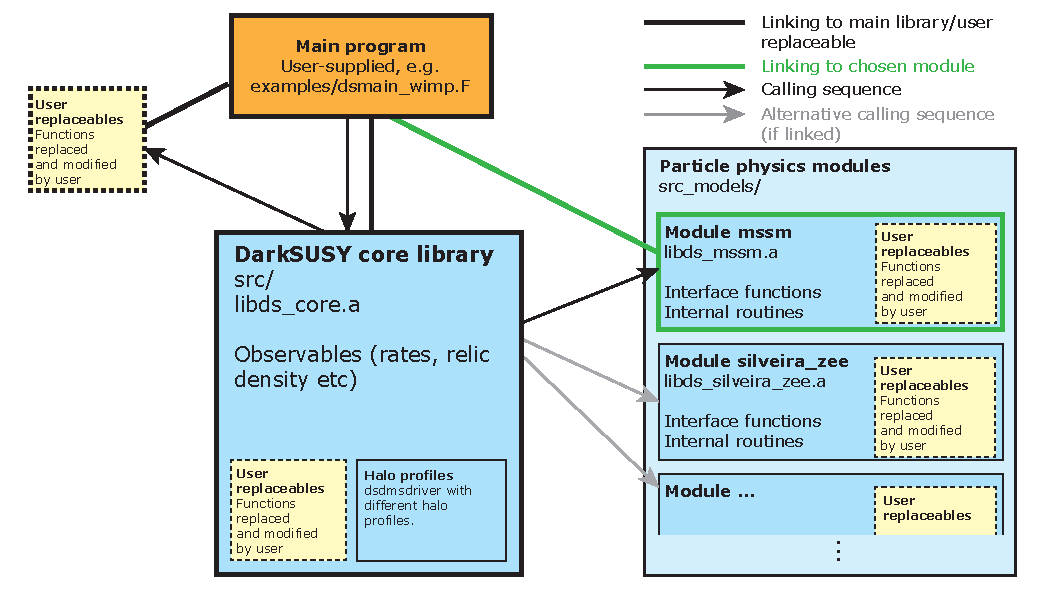
\includegraphics[width=\textwidth]{fig/ds6-structure-v6}
\vspace{-0.5cm}
\caption{Conceptual illustration of how to use \ds. The main program links
to both  the main library, \code{ds\_core}, and to \emph{one} of the available particle 
physics modules. User-replaceable functions are optional and may be linked to directly 
from the main program, or indirectly by including them in the various libraries. 
See \code{examples/dsmain\_wimp.F} for an example of a main program that demonstrates
typical usage of \ds\ for different particle physics modules.}
\label{fig:concept}
\end{figure}
%%%%%%%%%%%%%%%%%%%%%%%%%%		


%%%%%%%%%%%%%%%%%%%%%%%%%%
\begin{table}[t!]
%\centering
%\begin{tabular}[l]{l|l}
%subdirectory name & description\\
%\hline
%\code{src/ini} & Initialization routines\\
%\code{src/ge} & General utility functions of the main library\\[1ex]
%
%\code{src/an\_yield} & Simulated yield tables, e.g.~from $\bar bb$ final states\\
%\code{src/cr\_axi} & (Anti-)nucleon propagation routines for a generic 
%                               \\&axially symmetric diffusive halo\\
%\code{src/cr\_dmd} & Dark matter density profiles\\
%\code{src/cr\_gamma} & Gamma-ray routines, line-of-sight integrations etc.\\
%\code{src/cr\_ge} & general, auxiliary functions needed by cosmic ray routines\\
%\code{src/cr\_ps} & Positron propagation routines\\[1ex]
%
%\code{src/se\_aux} & Auxiliary routines needed by capture rate routines\\
%\code{src/se\_yield}& Simulated neutrino yield tables from the center of the Sun or Earth\\
%\code{src/se\_ic}& Neutrino flux likelihood calculations, using IceCube data\\
%\code{src/se\_mod} & Density and composition models for the Sun and the
%Earth\\
%\code{src/se\_nu} & Capture rate for dark matter in the Sun and in the Earth,
%\\& as well as neutrino fluxes from the center of Sun and Earth\\[1ex]
%
%\code{src/dd} & Direct detection routines\\[1ex]
%
%\code{src/kd} & Kinetic decoupling\\
%\code{src/rd} & Relic density\\[1ex]
%
%\code{src/xCERN} & numerical routines from the CERN library \cite{?} \\
%\code{src/x...} & Other contributed external code 
%            \\ & (currently \code{cmlib} \cite{?}, \code{diag} \cite{?} and \cod%e{galprop} \cite{?})\\
%\end{tabular}
\begin{tabular}{lp{10cm}}
{\bfseries Subdirectory} & {\bfseries } \\
{\bfseries name} & {\bfseries Description} \\
\hline
\ft{an\_yield} & Annihilation yields in the halo -- yields from simulations
 \\[0.5ex]
\ft{aux} & General routines
 \\[0.5ex]
\ft{aux\_xcernlib} & CERN routines needed by DarkSUSY
 \\[0.5ex]
\ft{aux\_xdiag} & Diagonalization routines
 \\[0.5ex]
\ft{aux\_xquadpack} & CMLIB routines needed by DarkSUSY
 \\[0.5ex]
\ft{cr\_aux} & Cosmic rays -- general
 \\[0.5ex]
\ft{cr\_axi} & Cosmic rays -- diffusion routines for axisymmetric distributions
 \\[0.5ex]
\ft{cr\_gamma} & Cosmic rays -- Gamma fluxes
 \\[0.5ex]
\ft{cr\_nu} & Cosmic rays -- Neutrino fluxes
 \\[0.5ex]
\ft{cr\_ps} & Cosmic rays -- point sources
 \\[0.5ex]
\ft{dd} & Direct detection
 \\[0.5ex]
\ft{dmd\_astro} & Astrophysical source functions
 \\[0.5ex]
\ft{dmd\_aux} & Auxiliary functions for dark matter distribution routines
 \\[0.5ex]
\ft{dmd\_mod} & Dark matter distributions
 \\[0.5ex]
\ft{dmd\_vel} & Dark matter velocity distributions
 \\[0.5ex]
\ft{fi} & \comment{Missing file: src/fi/DOC-name.tex} \\[0.5ex]
\ft{ini} & Initialization routines
 \\[0.5ex]
\ft{kd} & Kinetic decoupling
 \\[0.5ex]
\ft{rd} & Relic density
 \\[0.5ex]
\ft{se\_aux} & Auxiliary routines for WIMP annihilation in the Sun/Earth
 \\[0.5ex]
\ft{se\_mod} & Sun and Earth models
 \\[0.5ex]
\ft{se\_nu} & Capture and annihilation in the Sun/Earth
 \\[0.5ex]
\ft{se\_yield} & Yields from annihilation in the Sun/Earth
 \\[0.5ex]
\ft{si} & Self-interactions \\[0.5ex]
\ft{ucmh} & Ultra-compact mini-halos
 \\[0.5ex]
\hline
\end{tabular}
\caption{Organization of the main library  \code{ds\_core}: all functions and subroutines 
reside in the \code{src/} folder of the \ds\ installation, with the names of the subdirectories 
indicating the subject area. (Note: this table is automatically generated from the actual directory structure in \code{src/}.)
}
\label{tab:dsmain}
\end{table}
%%%%%%%%%%%%%%%%%%%%%%%%%%		


\section{The main \ds\ library \code{ds\_core}}

\index[routines]{ds\_core} As introduced above, the main library is in some sense the heart of the new \ds\,,
offering all the functionality that a user typically would be interested in without having 
explicitly to refer to specific characteristics of a given particle physics model (after
initialization of such a model).
 The main library thus contains routines for, e.g., 
cosmic ray propagation, solar models, capture rates for the Sun/Earth, a 
Boltzmann solver for the relic density calculation, yield tables from annihilation/decay etc. 
None of the routines in the main library contains any information about the particle 
physics module. Instead any information needed is obtained by calling a required 
function that resides in the  particle physics module which is linked to (see below). 

The source code for all functions and subroutines in the main library can be found in the 
\code{src/} directory of the \ds\ installation folder, with subdirectory names indicating  
subject areas as summarized in Table \ref{tab:dsmain}.


%%%%%%%%%%%%%%%%%%%%%%%%%%%%%%%%%%%%%%%%%%%%%%%%%%%%%%%%%%
%%%%%%%%%%%%%%%%%%%%%%%%%%%%%%%%%%%%%%%%%%%%%%%%%%%%%%%%%%
\section{Particle physics modules}
\label{sec:particle_modules}

\index{particle physics modules} The particle physics modules contain the parts of the code that 
depend on the respective 
particle physics model. Examples are cross section calculations, yield calculations etc. 
The routines in the particle physics module have access to all routines in 
\code{ds\_core}, whereas the reverse is in general not true (with the exception of a very limited 
set of interface functions that each particle module provides). 

\ds\ 5 and earlier was primarily used for supersymmetric, and neutralino DM, and those 
parts of the code now reside in the MSSM module \code{mssm}. However, many people 
used \ds\ even before for e.g.\ a generic WIMP setup, which was doable for parts of the 
code, but not all of it. We now provide a generic WIMP module \code{generic\_wimp} that 
can be used for these kinds of calculations in a much more general way. 
 In a similar spirit,
we also provide a module \code{generic\_decayingDM} for phenomenological studies
of decaying DM scenarios. As an example for an actual particle physics model
other than supersymmetry,
\ds\  furthermore includes a module \code{silveira\_zee} which implements the
DM candidate originally proposed by Silveira and Zee \cite{Silveira:1985rk} and which 
now is often
referred to as Scalar Singlet DM \cite{McDonald:1993ex,Burgess:2000yq,Cline:2013gha}.
%We also provide a module for universal extra dimensions, \code{ued}. It is far from complete, 
%as of version 6 of the code, but serves to illustrate that even if you do 
% not have the complete module, you can still use \ds\ for calculations where your module 
% provides required functions beyond simple dummy versions.
We also include an empty model, \code{empty}, 
which is of course not doing any real calculations, but contains (empty versions of) all
interface functions that the core library is aware of -- which is very useful for debugging and
testing purposes. Designing new particle modules is 
a straight-forward exercise, see below, and it is generally a good idea 
to start with the most similar module that is already available.

A list of the currently available particle physics modules is given in table~\ref{tab:modules},
and the source code for the particle modules can be found in the \code{src\_models/} 
directory of the \ds\ installation folder, each of the subdirectories 
(e.g.~\code{src\_models/mssm/}, \code{src\_models/generic\_wimp/}) typically 
reflecting a (sub)subdirectory structure analogous to what is shown in Table \ref{tab:dsmain}
for the core library. 
%
Many dark matter models, furthermore, constitute only relatively simple extensions to the 
standard model, inheriting most of its structure. For convenience,
we therefore also provide various auxiliary routines, in \code{src\_models/common/sm}, that each particle module 
automatically has access to, and which return basic standard model quantities like, e.g., the masses
of standard model particles and their running (so additional BSM effects have to be implemented in the
respective particle module).


\begin{table}[t!]
\begin{tabular}{llp{8cm}}
\multicolumn{3}{l}{\bfseries Particle physics modules} \\
\cline{1-3}
{\bfseries Module} & {\bfseries Short} & {\bfseries } \\
{\bfseries No.} & {\bfseries name} & {\bfseries Description} \\
\hline
1 & \ftb{common} & Basic principles and common routines \\[0.5ex]
2 & \ftb{empty} & The empty model \\[0.5ex]
3 & \ftb{generic\_decayingDM} & Generic decaying dark matter \\[0.5ex]
4 & \ftb{generic\_wimp} & Generic WIMPs \\[0.5ex]
5 & \ftb{mssm} & The Minimal Supersymmetric Standard Model \\[0.5ex]
6 & \ftb{silveira\_zee} & Silveira-Zee (Scalar Singlet) \\[0.5ex]
7 & \ftb{vdSIDM} & Self-Interacting Dark Matter \\[0.5ex]
\hline
\end{tabular}
\caption{List of particle physics modules currently available in \code{src\_models}. (Note: this table is automatically generated from the actual content of \code{src\_models}.)}
\label{tab:modules}
\end{table}


\subsection{Using a particle physics module}
%%%%%%%%%%%%%%%%%%%%%%%%%%%%%%%%%%%%%%%%%%%%%%%%%%%%%%%%%%%%%%%%%%%%

How to use a particle physics module obviously depends on how it is implemented,
and in principle there are no formal requirements on how this should be done -- as long as the 
provided interface functions are correctly set up, see Section \ref{sec:interface} further down.
The one subroutine that {\it is} required to exist, however, is
\begin{verbatim}
dsinit_module
\end{verbatim}
This is called directly from \code{dsinit}, and must be the first call to the particle module 
as it initializes all general settings and relevant common block variables. 

While there is no required structure otherwise, there is a typical workflow associated to using
a particle physics module in a main program. First, one needs to initialize a given model
by specifying its model parameters. This is done by routines like
\begin{verbatim}
dsgivemodel...
\end{verbatim}
A call to \code{dsgivemodel\_decayingDM}, e.g., allows to enter the defining parameters for 
a DM model in the \code{generic\_decayingDM} module, while \code{dsgivemodel\_25} allows 
to enter the parameters for pMSSM model with 25 parameters in the \code{mssm} module.
The next step is then typically a call to
\begin{verbatim}
dsmodelsetup
\end{verbatim}
in order to transfer the model parameters to common blocks and calculate basic quantities like
masses and couplings. Once a model is set up like this, a main program can use the full
functionality of \ds\ supported by the respective module.


\subsection{Adding a new particle physics module}


To create a new particle physics module, the easiest way is to start from an existing one as a template 
and create a new one from that one. To help you in this process we provide a script 
\code{scr/make\_module.pl} that takes two arguments, the module you want to start from and 
the new one you 
want to create (for further instructions, just call the script without arguments). 
It will then copy the module to a new one, change its name 
throughout the module and make sure that it is compiled by the makefiles and included properly when 
requested by the main programs. If you specify the option \code{-i} only interface functions will be copied 
(which creates a cleaner starting point, but also will most likely not compile without modifications). When 
creating a new module this way, the best is to copy from a module that is as similar as possible to your 
new model. If you want a clean setup, you can always copy from the \code{empty} module. If you want something more phenomenological that has a basic framework for calculating observables, starting from the \code{generic\_wimp} or \code{generic\_decayingDM} might be a good idea. A general
advice is to view the modules we provide as a starting point as inspiration for your new modules.

Even though a particle physics module does not need to include all interface functions (which ones 
are needed only depends on the observables you try to calculate in your main programs), it needs to provide 
an initialization routine 
\code{dsinit\_module.f}. This routine should set a global variable \code{moduletag} to the name of 
the module so that routines that need to check if the correct module is loaded can do so. When using the 
script \code{scr/make\_module.pl} this routine is always created and \code{moduletag} set as it should.


Note that the script \code{scr/make\_module.pl} only provides the framework in the configure script and makefiles (or rather makefile.in's) to make sure your module is compiled. It does \emph{not} create a main program that uses your module, that is up to you. A good starting point for that can either be e.g.\ \code{dsmain\_wimp.F} in examples that already contain different blocks for different modules (controlled by pre-compiler directives, see the code for more details). Another option is to use any of the example programs in \code{examples/aux} as a starting point. 

To make upgrading to new \ds\ versions as smooth as possible, we advice to create your own folder with your main programs, using e.g.\ the \code{makefile} in \code{examples/aux} as a starting point. Don't modify any of the \ds\ \code{makefile}s directly as they are overwritten every time you run \code{configure}, see Section~\ref{sec:makeownmain} for more details.

Note that for the \code{scr/make\_module.pl} script to work you need to have \code{autoconf} installed as the script adds your new module to \code{configure.ac} and runs \code{autoconf} to create a new \code{configure} script.

%%%%%%%%%%%%%%%%%%%%%%%%%%%%%%%%%%%%%%%%%%%%%%%%%%%%%%%%%%
%%%%%%%%%%%%%%%%%%%%%%%%%%%%%%%%%%%%%%%%%%%%%%%%%%%%%%%%%%
\section{Halo models}
\label{sec:halo_general}

Several routines in the core library need to know which DM halo should be adopted for the 
calculations. With this \ds\ version, we introduce a new and flexible scheme that avoids 
pre-defined hardcoded functions to describe the DM density profiles, and allows to 
consistently define different DM targets at the same time. For convenience, we still provide
several pre-defined options for such halo parameterizations, and the user can choose 
between, e.g., the Einasto \cite{1965TrAlm...5...87E} and the Navarrow-Frenk-White profile 
\cite{Navarro:1995iw}, or read in any tabulated axi-symmetric (or spherically symmetric) profile. 
On a {\it technical} level, the halo models are handled by the \code{dsdmsdriver} routine which 
contains a database of which  halo profiles the user has set up, and consistently passes this
information to all parts in the code where it is needed.\footnote{
From a technical point of view, it is actually not  \code{dsdmsdriver} itself which acts as an interface
to the rest of the code, but the set of wrapper routines collected in \code{src/dmd\_astro} (which all call \code{dsdmsdriver}
in a specific way). Only those routines are called by 
cosmic-ray flux routines and other functions in \code{src}, never \code{dsdmsdriver} directly.
The routines in  \code{src/dmd\_astro} therefore provide examples of functions that {\it cannot be
replaced} individually in a consistent way, but only as a whole set (along with \code{dsdmsdriver},
in case the user wants to change the structure of the driver itself).  
} 

We provide detailed hands-on examples on how to use this system by a set of example
programs \code{DMhalo\_*.f}, see Section \ref{sec:aux_ex}. For further details, we refer
to Section \ref{sec:halo} of this manual.


%%%%%%%%%%%%%%%%%%%%%%%%%%%%%%%%%%%%%%%%%%%%%%%%%%%%%%%%%%
%%%%%%%%%%%%%%%%%%%%%%%%%%%%%%%%%%%%%%%%%%%%%%%%%%%%%%%%%%
\section{Interface functions}
\label{sec:interface}

\index{interface functions} Interface functions are functions that routines in \code{ds\_core} might need to call, and
which therefore every particle physics module should contain if that particular observable is requested. 
Examples of interface functions include \code{dsddsigma} that returns the equivalent DM nucleus cross section, \code{dscrsource} that 
returns the source term for DM-induced cosmic rays (relevant for indirect detection),
\code{dsanxw} that returns the invariant annihilation rate (in the case of WIMPs), etc.
 All interface functions are found by looking in the empty module, and always contain the 
 keyword `interface' in the function or subroutine header.

If a particle physics module contains the full set of interface functions, all
routines in the main \ds\ code should work. However, this is not needed to set up a paticle physics module. E.g.\ a generic WIMP model does not need to have decay rates set up. If a routine in the main \ds\ routines is called that rely on this interface being present, an error will be thrown when trying to compile your code. This of course applies to all interface functions, not just unphysical ones. E.g.\ if you are only interested in the relic density for a new particle physics module, you do not need to set up scattering rates, cosmic ray source functions, etc.

In Tab.~\ref{tab:if}, we provide the complete list of interface functions currently implemented in \ds,
along with a brief description. For more details, consult the headers of these files.

\bigskip

\begin{table}[!h]
\begin{tabular}{llp{3cm}p{6cm}}
 & {\bfseries Appear in} & {\bfseries } & {\bfseries } \\
{\bfseries Routine} & {\bfseries modules} & {\bfseries Used by} & {\bfseries Description} \\
\hline
\ftb{dsacbnd} & 2, 5 &  &  Check collider bounds \\[0.5ex]
\ftb{dsanwx} & 2, 4, 5, 6, 7 & rd &  Self-annihilation invariant rate \\[0.5ex]
\ftb{dscrsource\_line} & 2, 3, 4, 5, 6, 7 & cr\_axi &  Source term for monochromatic contributions from dark matter \\[0.5ex]
\ftb{dscrsource} & 2, 3, 4, 5, 6, 7 & cr\_axi, cr\_gamma, cr\_nu, ucmh &  Source term for dark matter induced cosmic rays \\[0.5ex]
\ftb{dsddgpgn} & 2, 4, 5, 6, 7 & se\_nu &  Four fermion couplings. \\[0.5ex]
\ftb{dsddsigma} & 1, 2 & dd &  UNpolarized *equivalent* WIMP nucleus cross section including form factors \\[0.5ex]
\ftb{dsdmspin} & 2, 3, 4, 5, 6, 7 & se\_nu &  dark matter spin \\[0.5ex]
\ftb{dsinit\_module} & 2, 3, 4, 5, 6, 7 & ini &  Intialzation of module \\[0.5ex]
\ftb{dskdm2simp} & 2, 4, 5, 6, 7 & kd &  Scattering amplitude squared for zero momentum transfer \\[0.5ex]
\ftb{dskdm2} & 2, 4, 5, 6, 7 & kd &  Full scattering amplitude squared at zero momentum transfer \\[0.5ex]
\ftb{dskdparticles} & 2, 4, 5, 6, 7 & kd &  Initalization of kinetic decoupling for module \\[0.5ex]
\ftb{dsmodelsetup} & 2, 3, 4, 5, 6, 7 &  &  Sets up a new particle physics model in module \\[0.5ex]
\ftb{dsmwimp} & 2, 3, 4, 5, 6, 7 & cr\_axi, kd &  WIMP mass \\[0.5ex]
\ftb{dsrddofDS} & 2, 7 & rd &  Relativistic BSM degrees of freedom  \\[0.5ex]
\ftb{dsrdparticles} & 2, 4, 5, 6, 7 & rd &  Particles included in relic density calculation (coannihilations, resonances and thresholds) \\[0.5ex]
\ftb{dsseyield} & 2, 4, 5, 6, 7 & se\_nu &  Yields from annihilation in the Sun/Earth \\[0.5ex]
\ftb{dssigmav0tot} & 2, 4, 5, 6, 7 & cr\_axi, se\_nu &  Total annihilation cross section at $v=0$ \\[0.5ex]
\ftb{dssisigtm} & 2, 7 & si &  momentum-transfer cross section \\[0.5ex]
\hline
\end{tabular}
 \smallskip
\caption{Table of interface functions, which modules that contain them (with numbering from table~\ref{tab:modules}, where they are used and a short description of them. (Note: this table is automatically generated from scanning through the particle physics modules in \code{src\_models}. The description is taken from the \code{empty} module routine headers.)}
\label{tab:if}
\end{table}


%%%%%%%%%%%%%%%%%%%%%%%%%%%%%%%%%%%%%%%%%%%%%%%%%%%%%%%%%%
%%%%%%%%%%%%%%%%%%%%%%%%%%%%%%%%%%%%%%%%%%%%%%%%%%%%%%%%%%
\section{Commonly used functions}

\index{commonly used functions}Routines that we believe are particularly  useful for most users to call, we denote 
as \emph{commonly used functions}. A list of the commonly used functions in the main \ds\ library in \code{src} is 
shown in Table \ref{tab:culist}. The routines are described in more detail in their corresponding chapters in part II of 
this manual, as indicated in the table \ref{tab:culist}. 

\bigskip

\begin{table}[!h]
\begin{tabular}{lp{8.5cm}l}
{\bfseries Routine} & {\bfseries Description} & {\bfseries Chapter} \\
\hline
\ftb{dsanyield\_sim} \index[routines]{dsanyield\_sim} &  Simulated particle yields & \ref{ch:src/an_yield} \\
\ftb{dsdbdphidtaxi} \index[routines]{dsdbdphidtaxi} &  Local galactic differential antideuteron flux from dark matter & \ref{ch:src/cr_axi} \\
\ftb{dsepdphidpaxi} \index[routines]{dsepdphidpaxi} &  Local galactic differential positron flux from dark matter & \ref{ch:src/cr_axi} \\
\ftb{dspbdphidtaxi} \index[routines]{dspbdphidtaxi} &  Local galactic differential antiproton flux from dark matter & \ref{ch:src/cr_axi} \\
\ftb{dscrgaflux\_line\_v0ann} \index[routines]{dscrgaflux\_line\_v0ann} &  Flux of monoenergetic gamma-rays from annihilation in the halo,  in the limit of zero relative velocity & \ref{ch:src/cr_gamma} \\
\ftb{dscrgaflux\_v0ann} \index[routines]{dscrgaflux\_v0ann} &  Flux of gamma-rays from annihilation in the halo, in the limit of zero relative velocity & \ref{ch:src/cr_gamma} \\
\ftb{dsgafluxsph} \index[routines]{dsgafluxsph} &  gamma-rays from decay/annihilation from halo specified by halo label & \ref{ch:src/cr_gamma} \\
\ftb{dscrmuflux\_v0ann} \index[routines]{dscrmuflux\_v0ann} &  Flux of neutrino-induced muons from WIMP annihilation in the halo & \ref{ch:src/cr_nu} \\
\ftb{dsdddrde} \index[routines]{dsdddrde} &  Differential WIMP-nucleus recoil rates & \ref{ch:src/dd} \\
\ftb{dsddhelp} \index[routines]{dsddhelp} &  help with options for scattering cross sections & \ref{ch:src/dd} \\
\ftb{dsddset} \index[routines]{dsddset} &  Set parameters for scattering cross sections & \ref{ch:src/dd} \\
\ftb{dsddsigmanucleon} \index[routines]{dsddsigmanucleon} &  Calculate nuclear cross sections & \ref{ch:src/dd} \\
\ftb{dsdfactor} \index[routines]{dsdfactor} &  D-factor (l.o.s. integral for decaying DM) & \ref{ch:src/dmd_aux} \\
\ftb{dsjfactor} \index[routines]{dsjfactor} &  J-factor (l.o.s. integral for annihilating DM) & \ref{ch:src/dmd_aux} \\
\ftb{dsdmdselect\_halomodel} \index[routines]{dsdmdselect\_halomodel} &  select between halo models in the halo repository & \ref{ch:src/dmd_mod} \\
\ftb{dsdmdset\_halomodel} \index[routines]{dsdmdset\_halomodel} &  add an existing halo model to halo repository & \ref{ch:src/dmd_mod} \\
\ftb{dsinit} \index[routines]{dsinit} &  Initialize DarkSUSY (should always be called) & \ref{ch:src/ini} \\
\ftb{dskdmcut} \index[routines]{dskdmcut} &  Cutoff mass in linear power spectrum & \ref{ch:src/kd} \\
\ftb{dskdtkd} \index[routines]{dskdtkd} &  Kinetic decoupling temperature & \ref{ch:src/kd} \\
\ftb{dsrdomega} \index[routines]{dsrdomega} &  Calculate the relic density $\Omega h^2$ of a dark matter particle & \ref{ch:src/rd} \\
\ftb{dssenu\_rates} \index[routines]{dssenu\_rates} &  Rates of neutrinos and neutrino-induced leptons and hadronic showers from WIMP annihilations in the Sun/Earth & \ref{ch:src/se_nu} \\
\ftb{dssisigtmav} \index[routines]{dssisigtmav} &  velocity-averaged momentum-transfer cross section & \ref{ch:src/si} \\
\hline
\end{tabular}
\caption{List of commonly used functions and subroutines. (Note: this table is automatically generated from the routines in \code{src} that have the commonly used tag in their header.)}
\label{tab:culist}
\end{table}


\section{Replaceable functions}
\label{sec:replaceable}
\index{replaceable functions}
The concept of replaceable functions introduces the possibility to replace a \ds\ routine with one of your own. The way it works is that the user-provided function will be linked 
when you make your main program instead of the \ds\ default one. If, for example, you want to 
replace the yields from a typical final state of DM annihilation or decay (like $\bar bb$)
with a new function of your own -- e.g.~because you are interested in comparing the tabulated
{\sf Pythia} \cite{Sjostrand:2006za} yields with those provided by PPPC \cite{Cirelli:2010xx} --  
you create your own version of the routine \code{dsanyield\_sim} and let \ds\ use this one 
instead.  To help you with this setup, 
we provide tools that can create (or delete) a replaceable function from any \ds\ function 
and set up the makefiles to use this user-supplied function instead. We also provide a
simply way of managing large `libraries' of user-supplied functions, via a list imported 
by the makefiles, where the user can determine on the fly which user-replaceable 
functions should be included and which ones should not.  Note that both routines in 
\code{ds\_core} and in any of the particle physics modules can be replaced in this way,
including interface functions. There is also a possibility for the particle physics modules to replace a
function in the core library. This is not used often, but is used e.g.\ for the function \code{dsrdxi.f} (which gives a possibility to have different dark matter and background temperatures in the early Universe).

There is also a simple way to bypass this system  -- indicated in the left-most part of Fig.~\ref{fig:concept} --
by directly linking to the user-supplied function only when making the main program. 
 For an explicit example, see (the makefile for) \code{generic\_wimp\_oh2.f}.

%%%%%%%%%%%%%%%%%%%%%%%%%%%%%%%%%%%%%%%%%%%%%%%%%%%%%%%%%%%%
%%% Here comes docs/I04-Comparison.tex %%%
%%%%%%%%%%%%%%%%%%%%%%%%%%%%%%%%%%%%%%%%%%%%%%%%%%%%%%%%%%%%
%%%%%%%%%%%%%%%%%%%%%%%%%%%%%%%%%%%%%%%%%%%%%%%%%%%%%%%%%%%%%%%%%%%%
\chapter{Comparison to previous \ds\ versions}
\label{ch:translation}

For those \ds\ users who are familiar with previous version of the code, the main 
structural difference introduced with \ds\ 6.0 is a highly modular setup that allows to 
fully disentangle the astrophysics-related parts from those that rely on a specific particle
physics model (see Chapter 
\ref{ch:philosophy} for a detailed description). There are also many new or significantly 
improved physics capabilities introduced after version 5 and 4 \cite{ds4} -- including 
electroweak and strong corrections to DM annihilation, improved routines to solve
the Boltzmann equation for chemical and kinetic decoupling, and a new framework to handle 
the propagation of cosmic rays. For a detailed list of those new features, we refer to the 
publication describing this release of the code \cite{ds6}.


One technical aspect that has changed are the particle codes ($k$-variables), which are 
now treated as (module-)internal codes. They can be used by the particle physics module if the 
module so wishes, but the interface functions and routines in \code{ds\_core} instead 
use PDG codes when referring to particles.

In the course of re-organizing the code, it also became necessary to re-name some of the 
basic functions and subroutines that existed in earlier versions and which users may have
become familiar with. For convenience, we therefore list below, in Table \ref{tab:translation},
 the most commonly used functionalities in version 4 and 5 that have changed in name or 
 usage with the present version of the code.


%%%%%%%%%%%%%%%%%%%%%%%%%%
%\begin{table}[t!]
%\centering
%\begin{tabular}[l]{lll}
\captionsetup{width=\textwidth}
\begin{longtable}{ p{.33\textwidth}  p{.22\textwidth}  p{.35\textwidth} } 
\\[1ex]
routine name up to \ds\ 5 & new routine name & comments\\
\hline
\code{dshmset} & \code{dsdmdset\_halomodel} &  \parbox[t]{5.5cm}{Setting up and refering to DM
halos has fundamentally changed. See Section \ref{sec:halo_general} for an overview and all Chapters with names
containing  \code{src\_dmd} in Part II of the manual for more details.} \vspace*{1.5ex}\\
%
\code{dshmj} & \code{dsjfactor} &  \parbox[t]{5.5cm}{Line-of-sight integrals now take a halo label as input, and can be
computed for various objects at the same time.} \vspace*{1.5ex}\\
%
\code{dssusy} & [\code{dsmodelsetup}] &  \parbox[t]{5.5cm}{Setting up a model (calculating the mass spectrum,  
relevant 3-particle vertices etc.) now depends on the particle module implementation.} \vspace*{1.5ex}\\
%
\parbox[t]{4cm}{\code{dsmhtkd}\\\code{dsmhmcut}} & \parbox[t]{4cm}{\code{dskdtkd}\\\code{dskdmcut}} 
&  \parbox[t]{5.5cm}{The 'microhalo' routines are now more properly referred to as 'kinetic decoupling' routines.} \vspace*{1.5ex}\\
%
\code{dshmrescale\_rho} & ---& \parbox[t]{5.5cm}{A mismatch between local halo density and DM abundance 
for a given \ds\ module is no longer hidden as a rescaling factor in a common block. Instead, such factors 
typically enter as explicit parameters in direct and indirect detection routines.} \vspace*{1.5ex}\\
%
\code{dshaloyield} & [\code{dsanyield}] & \parbox[t]{5.5cm}{total cosmic ray yield from {\it neutralino} annihilation}
\vspace*{1.5ex}\\
%
\code{dshayield} & \code{dsanyield\_sim} &  \parbox[t]{5.5cm}{simulated cosmic ray yields from individual annihilation/decay channels to SM particles. 
Note that internal channel codes are now replaced with PDG codes of the final state particles as input.}
\vspace*{1.5ex}\\
%
\code{dshrgacontdiff} & \code{dsgafluxsph} &  \parbox[t]{5.5cm}{Gamma-ray flux routines now work seamlessly together with both the new halo setup and the modular particle physics structure.}
\vspace*{1.5ex}\\
%
\code{dshrgaline} & \parbox[t]{4cm}{\code{dscrgaflux\_line\_v0ann}\\\code{dscrgaflux\_dec}} & \parbox[t]{5.5cm}{Gamma-ray line routines now return both number, energies and widths of all such signals that are present in the current particle setup.}
\vspace*{1.5ex}\\
%
\parbox[t]{4cm}{\code{dshrpbardiff}\\\code{dshrdbardiff}\\\code{dsepdiff}} 
& \parbox[t]{4cm}{\code{dspbdphidtaxi}\\\code{dsdbdphidtaxi}\\\code{dsepdphidpaxi}} 
&  \parbox[t]{5.5cm}{Cosmic-ray propagation routines have been re-written 
from scratch. They are now much more flexible and can be used for any axisymmetric halo/diffusion model.}
\vspace*{1.5ex}\\
%
\code{dsntrates} & \code{dssenu\_rates} &  \parbox[t]{5.5cm}{Neutrino rates from inside the sun or earth}
\vspace*{1.5ex}\\
%
\code{dshrmuhalo} &  \parbox[t]{4cm}{\code{dscrmuflux\_v0ann}\\\code{dscrmuflux\_v0ann}} 
&  \parbox[t]{5.5cm}{Neutrino-induced muon flux from the halo
(for annihilating and decaying DM, respectively).}
\vspace*{1.5ex}\\
%

\hline
%\end{tabular}
\caption{`Translation table' for how the most commonly used functionalities in \ds\ version 5 and earlier have changed with the
present version of the code. Routines in parentheses, e.g.  [\code{dsanyield}], are no longer part of the \ds\ main library and only 
provided by specific particle physics modules. For more detailed descriptions of the new routines and functions, see the headers of the respective 
files. 
}
\label{tab:translation}
\end{longtable}
%\end{table}
%%%%%%%%%%%%%%%%%%%%%%%%%%		

%%%%%%%%%%%%%%%%%%%%%%%%%%%%%%%%%%%%%%%%%%%%%%%%%%%%%%%%%%%%
%%% Here comes docs/I05-OriginalReferences.tex %%%
%%%%%%%%%%%%%%%%%%%%%%%%%%%%%%%%%%%%%%%%%%%%%%%%%%%%%%%%%%%%
%%%%%%%%%%%%%%%%%%%%%%%%%%%%%%%%%%%%%%%%%%%%%%%%%%%%%%%%%%%%%%%%%%%%
\chapter{Original articles}
\label{sec:DS_papers}

A large part of the routines in the present \ds\ version have been implemented 
in the context of original research work. Therefore, when using those routines, 
please give proper credit not only to the main \ds\ paper \cite{ds4,ds6} but also
to the relevant articles in the following list:

\bigskip

  \begin{description}
    \item[Relic density] P.~Gondolo and G.~Gelmini, Nucl.\ Phys. 
         {\bfseries B360} (1991) 145 \cite{Gondolo:1990dk}; J.~Edsj{\"o} and P.~Gondolo, 
         Phys.\ Rev.\ {\bfseries D56} (1997) 1879 \cite{Edsjo:1997bg}; J. Edsj\"o, 
         M. Schelke, P. Ullio and P. Gondolo, JCAP {\bfseries 04} (2003) 001 \cite{Edsjo:2003us}.
    \item[Kinetic decoupling and microhalos]
      T.~Bringmann, NJP {\bfseries 11} (2009) 10527 \cite{Bringmann:2009vf}.
    \item[Continuous gamma-rays]
      L.~Bergstr{\"o}m, J.~Edsj{\"o} and P.~Ullio, Phys.\ Rev.\ {\bfseries D58} (1998) 083507 \cite{Bergstrom:1998zs}.
    \item[Neutrino telescopes]
       L.~Bergstr{\"o}m, J. Edsj{\"o} and P. Gondolo, Phys.\ Rev.\
      {\bfseries D58} (1998) 103519 \cite{Bergstrom:1998xh}.
    \item[Positrons]
      E.A.~Baltz and J.~Edsj{\"o}, Phys.\ Rev.\ {\bfseries D59} (1999) 023511 \cite{Baltz:1998xv}.
    \item[Antiprotons]
      L.~Bergstr{\"o}m, J.~Edsj{\"o} and P.~Ullio, ApJ {\bfseries 526} (1999) 215 \cite{Bergstrom:1999jc}.
    \item[QCD corrections to DM annihilation]
      T.~Bringmann, A.~J.~Galea, P.~Walia,  Phys.Rev. {\bfseries D93} (2016) 043529 \cite{Bringmann:2015cpa}.
    \item[General MSSM, direct detection] L.~Bergstr{\"o}m and
      P.~Gondolo, Astrop. Phys. {\bfseries 5} (1996) 263 \cite{Bergstrom:1995cz}.
    \item[Gamma lines from supersymmetric DM]
      L.~Bergstr{\"o}m and P.~Ullio, Nucl. Phys. {\bfseries B504} (1997) 27 \cite{Bergstrom:1997fh};
    P.~Ullio and L.~Bergstr\"om, Phys. Rev.\ {\bfseries D57} (1998) 1962 \cite{Ullio:1997ke}.
    \item[Internal bremsstrahlung in the MSSM ($\gamma$ and $e^+$)]
      T.~Bringmann, L.~Bergstr{\"o}m and J.~Edsj{\"o}, JHEP {\bfseries 0801} (2008) 049 \cite{Bringmann:2007nk};
       L.~Bergstr{\"o}m, T.~Bringmann and J.~Edsj{\"o}, Phys.Rev.\ {\bfseries D78} (2008) 103520 \cite{Bergstrom:2008gr}.
    \item[MSSM Electroweak corrections to indirect detection yields]
       T.~Bringmann and F.~Calore,  Phys.Rev.Lett.\ {\bfseries 112} (2014) 071301 \cite{Bringmann:2013oja};
       T.~Bringmann, F.~Calore, A.~J.~Galea and M.~Garny, JHEP\ {\bfseries 1709} (2016) 041 \cite{Bringmann:2017sko}.
  \end{description}

%%%%%%%%%%%%%%%%%%%%%%%%%%%%%%%%%%%%%%%%%%%%%%%%%%%%%%%%%%%%
%%% Here comes part Main DarkSUSY routines in src/
%%%%%%%%%%%%%%%%%%%%%%%%%%%%%%%%%%%%%%%%%%%%%%%%%%%%%%%%%%%%
\part{Main DarkSUSY routines in src/}


\chapter[an\_yield: Annihilation yields in the halo -- yields from simulations]{\codeb{an\_yield}:\\ Annihilation yields in the halo -- yields from simulations}
\label{ch:src/an_yield}

%%%%%%%%%%%%%%%%%%%%%%%%%%%%%%%%%%%%%%%%%%%%%%%%%%%%%%%%%%%%%%%%%%%%%%
\section{Annihilation in the halo, yields -- theory}

Here we calculate yields of different particles from annihilation of dark matter particles in the halo.

% \subsection{Cross sections and yields}

\comment{This description is outdated, and does not really reflect how we do things! So it's commented
out for the moment...}

%First, we need to define what we mean with a yield and a cross section. If we only have two-body final states, it is fairly straightforward to define the cross section and the yield per annihilation. The problem arises when we want to include also three-body final states, where we cannot consistently define a cross section for the two-body final states and the three-body ones. E.g.\ there will be an overlap between the final states $c\bar{c}$ and $c\bar{c}g$. We need to address what we mean with these concepts when we define the function(s) the particle physics module is required to provide. 
%
%We then in principle have three choices:
%\begin{enumerate}
%\item We define the cross section as the total cross section including three-body final states and define the yields per annihilation, were an annihilation is meant the annihilation described by the total cross section. In this case the sum of branching fractions over two-body final state will not necessarily equal 1. Also, the handling of possible overlap between two-body and three-body final states need to be handled in both the cross section and the yield routine.
%\item We define the cross section as the total cross section to all two-body final states and define the yields per annihilation to two-body final states. In this case the sum of branching fractions to all two-body final states should be one. Also, in this case, the possible overlap between two-body and final states only need to be considered in the yield routine.
%\item We don't provide the cross section and yields separately and instead just provide the source function which is essentially the product of the two.
%\end{enumerate}
%The last option is in principle the most general as it could also include decaying dark matter in a consistent way. It would also give the highest flexibility and the least risk of using the routines incorrectly. However, it would also be the one furthest away from how results from different experiments or properties of particle physics models are usually presented. Hence, even if this option is the most appealing from a physics point of view, we will not adopt it here. Instead we choose the first option as the concept of cross section in this case is closest to what it is usually considered to mean.

\subsection{Monte Carlo simulations}
\label{sec:ha-mcsim}

We need to evaluate the yield of different particles per WIMP annihilation.
The hadronization and/or decay of the annihilation products are
simulated with {\sc Pythia} \cite{Sjostrand:2006za} 6.426.
The simulations are done for a set of 18 WIMP
masses, $m_{\chi}$ = 10, 25, 50, 80.3, 91.2, 100, 150, 176, 200, 250,
350, 500, 750, 1000, 1500, 2000, 3000 and 5000 GeV\@. We tabulate the
yields and then interpolate these tables in \ds.

     The simulations are here
     simpler than those for annihilation in the Sun/Earth
    since we don't have a surrounding medium that can stop the
     annihilation products.  We here simulate for 8 `fundamental'
     annihilation channels $c\bar{c}$, $b\bar{b}$,
     $t\bar{t}$, $\tau^+\tau^-$, $W^+W^-$, $Z^0 Z^{0}$, $g g$ and
     $\mu^{+} \mu^{-}$. Compared to the simulations in the Earth and
     the Sun, we now let pions and kaons decay and we also let
     antineutrons decay to antiprotons. For each mass we simulate
     $2.5 \times 10^{6}$ annihilations and tabulate the yield of
     antiprotons, positrons, gamma rays (not the gamma lines),
     muon neutrinos and neutrino-to-muon conversion rates and the
     neutrino-induced muon yield, where in the last two cases the
     neutrino-nucleon interactions has been simulated with {\sc
     Pythia} as outlined in section~\ref{sec:nt-mcsim}


With these simulations, we can calculate the yield for any of these
particles for a given particle physics model. In \texttt{src}, we only include the channels that are actually simulated. In the different particle physics modules in \texttt{src\_model}, the summation over all possible final states and possibly more complex channels, like scalars decaying to other particles is done.

Note that simulations are typically done without specifying a particular polarization state of the final state particles. This is however not entirely correct as the possible polarization states will depend on the particle physics model we have. 

Even if the simulations are not performed in this more general way yet, we have set up the structure here to eventually provide the yields in this form. In particular the most general routine to calculate the yields from any of the simulated channels is \ftb{dsanyield\_sim\_ls}. Apart from the mass, energy and yield type, this routine also takes are arguments the PDG codes of the final state particles and the polarization state of the final state. In particular, you are required to provide the quantum numbers
\begin{eqnarray*}
j &=& \mbox{the quantum number for the total angular momentum} \\
P &=& \mbox{the parity of the final state}\\
l &=& \mbox{the quantum number for the orbital angular momentum in the final state} \\
s &=& \mbox{the quantum number for the total spin in the final state} 
\end{eqnarray*}
We want to move in a direction where this routine is the one that should be used. While getting there, we also provide a simpler routine which just gives the polarization state in terms of helcity and polarization, \ftb{dsanyield\_sim}. This routine takes the PDG code of the final state and the polarization as
\begin{itemize}
\item Left-handed or right-handed polarization for fermions. 
\item Longitudinal or transverse polarization for vector bosons.
\end{itemize}
This routine for simplicity assumes that the final state particles have the same polarization state.



\chapter[aux: General routines]{\codeb{aux}:\\ General routines}
\label{ch:src/aux}

%%%%%%%%%%%%%%%%%%%%%%%%%%%%%%%%%%%%%%%%%%%%%%%%%%%%%%%%%%%%%%%%%%%%
\section{General routines}

In \codeb{aux/}, we collect routines that are of general interest to
many other routines in \ds. E.g., we have routines to find elements in
arrays (used for interpolation), Bessel functions, error functions,
spline routines, etc.


\chapter[aux\_xdiag: Diagonalization routines]{\codeb{aux\_xdiag}:\\ Diagonalization routines}
\label{ch:src/aux_xdiag}

%%%%%%%%%%%%%%%%%%%%%%%%%%%%%%%%%%%%%%%%%%%%%%%%%%%%%%%%%%%%%%%%%%%%%%
\section{XDIAG}

This folder contains a set of routines to perform numerical
diagonalization of complex matrices. Even though analytical routines can be
used for up to $5 \times 5$ matrics, they tend to be numerically unstable for
matrices occuring in some particle physics models (for example supersymmetry).
Hence, we use numerical routines to perform the diagonalization instead.

\chapter[cr\_aux: Cosmic rays -- general]{\codeb{cr\_aux}:\\ Cosmic rays -- general}
\label{ch:src/cr_aux}

%%%%%%%%%%%%%%%%%%%%%%%%%%%%%%%%%%%%%%%%%%%%%%%%%%%%%%%%%%%%%%%%%%%%%%
\section{Cosmic Rays -- auxiliary routines}

This folder contains auxiliary functions needed by the cosmic ray routines. In particular,
it contains different versions of simple integration routines and a set of routines
to handle the correct setting and interpreting of labels for the tabulation of confinement times
and Green's functions needed for the calculation of cosmic ray fluxes.

\chapter[cr\_axi: Cosmic rays -- diffusion routines for axisymmetric distributions]{\codeb{cr\_axi}:\\ Cosmic rays -- diffusion routines for axisymmetric distributions}
\label{ch:src/cr_axi}

%%%%%%%%%%%%%%%%%%%%%%%%%%%%%%%%%%%%%%%%%%%%%%%%%%%%%%%%%%%%%%%%%%%%%%
\section{Cosmic ray propagation in axially symmetric halos}

There is a clean asymmetry between particles and antiparticles in the standard cosmic ray picture:
The bulk of cosmic rays -- protons, nuclei and electrons -- are mainly ``primary" species, i.e. particles
accelerated in astrophysical sources and then copiously injected in the interstellar medium;
``secondary" components, including antimatter, are instead produced in the interaction of primaries 
with the interstellar
medium during the propagation. It follows that there is a pronounced deficit of antimatter compared to matter 
in the locally measured cosmic ray flux (about 1 antiproton in $10^4$ protons). When considering instead a
source term due to DM annihilations or decays, a significant particle-antiparticle asymmetry is in general
not expected, and antiprotons, positrons and antideuterons turn out to be competitive indirect DM probes.

Charged particles propagate diffusively through the regular and turbulent components of Galactic magnetic 
fields. This makes it more involved for local measurements to track spectral and morphological imprints of 
DM sources than, e.g., for the gamma-ray and neutrino channels (though searches for spectral features
in CR positron fluxes still lead to very competitive limits \cite{Bergstrom:2013jra}).
In fact the transport of cosmic rays in the Galaxy is still a debated
subject: Most often one refers to the quasi-linear theory picture (with magnetic inhomogeneities as a perturbation 
compared to regular field lines) in which propagation can be described in terms of a (set of) equation(s) linear
in the density of a given species, containing terms describing diffusion in real space, diffusion in momentum
space (the so-called reacceleration), convective effects due to Galactic winds, energy or fragmentation
losses and primary and secondary sources (see, e.g., Ref.~\cite{Strong:2007nh} for a review).
Dedicated codes have been developed to solve numerically this transport equation, including GALPROP~\cite{Strong:1998pw}, DRAGON~\cite{Evoli:2016xgn} and PICARD~\cite{Kissmann:2014sia}. 

Here we follow instead a semi-analytical approach, analogous to that developed for the USINE 
code~\cite{Maurin:2001sj}. In particular, we model
the propagation of antiprotons and antideuterons by considering the steady state equation~\cite{Bergstrom:1999jc}
\begin{equation}
 \frac{\partial{N}}{\partial{t}} = 0 = \nabla \cdot
 \left(D\,\nabla N\right)
 - \nabla \cdot \left( \vec{u}\,N \right)
 - \frac{N}{\tau_N} + Q\,.
\label{eq:pbardiff}
\end{equation}
We solve it for situations where {\it i)} the diffusion coefficient $D$ can have an arbitrary dependence on the particle 
rigidity but can at most take two different values in the Galactic disc and in the diffusive halo, {\it ii)} the 
convective velocity $\vec{u}$ has a given fixed modulus and is oriented outwards and perpendicular to the disc,
{\it iii)} the loss term due to inelastic collisions has an interaction time $\tau_N$ which is energy dependent 
but spatially constant in the disc and going to infinity in the halo (corresponding to a constant target gas 
density in the disc and no gas in the halo), {\it iv)} the DM
source $Q$ is spatially axisymmetric and has a generic energy dendence. Under these
approximations and assuming, as is usually done, that the propagation volume is a cylinder centred at the disc 
and that particles can freely
escape at the boundaries of the diffusion region, Eq.~(\ref{eq:pbardiff}) can be solved analytically by expanding $N$
in a Fourier-Bessel series; the computation of the flux involves, at each energy, a sum over the series of 
zeros of a Bessel function of first kind and order zero, and a volume integral of the spatially dependent part in the axisymmetric
source term $Q$
 (basically the DM density $\rho_\chi$ for decaying DM and its square for pair annihilating DM) 
times a
weight function depending on the given zero in the series (see~\cite{Bergstrom:1999jc} for further details).

Since the path lengths for antiprotons and antideuterons are rather large, of the order of a few kpc, taking average
values for parameters in the transport equation rather than the more realistic modelling that can be implemented
in full numerical solutions, has no large impact in case of extended and rather 
smooth sources such as for DM. 
Eq.~(\ref{eq:pbardiff}) neglects reacceleration effects, which may in general be relevant at low energies
(rigidities below a few GV); however even this does not have a large impact in case of the species at hand,
see, e.g.,~\cite{Evoli:2011id} for a comparison of results with numerical and semi-analytical solutions for cosmic-ray
antiprotons. The power of our semi-analytic approach is that one can store values of 
the solution of the transport equation obtained by assuming 
a given mono-energetic source -- provided by 
the functions \code{dspbtdaxi} and \code{dsdbtdaxi} for, respectively, antiprotons and antideuterons -- and 
then apply these as weights to any particle source term $\mathcal{S}_n(E_f)$ as introduced above.
For antiprotons and antideuterons, this latter step is done in the functions that compute the local galactic differential 
fluxes from DM annihilation and decay, \code{dspbdphidtaxi} and \code{dsdbdphidtaxi}, respectively.
Note that while the outputs of \code{dspbtdaxi} and \code{dsdbtdaxi}  are labelled ``confinement time" in the code,
since they do have a dimension of time and scale the dependence between source and flux, one cannot trade
them for what is usually intended as confinement time for standard cosmic ray components, given that the
morphology of the DM source is totally different from supernova remnant distributions usually implemented
for describing ordinary primary components.

The structure we implemented gives a particularly clear advantage when the code is used to scan over many 
particle physics DM models, but only over a limited number of propagation parameters and DM density profiles.
For such an application,  it is useful to tabulate the 'confinement times' (returned by \code{dspbtdaxi} and 
\code{dsdbtdaxi}) over a predefined range of energy; this is
done in the functions \code{dspbtdaxitab} and \code{dsdbtdaxitab} when calling the flux routines with an appropriate
option (and only in case the DM halo profile currently active is within the halo profile database). 
Such tabulations  can be saved and re-loaded for later use; 
here the proper table association is ensured by 
a propagation parameter label setting system in analogy to the one implemented for the halo profile database. 
Computing such a table on the first call is rather CPU  consuming, especially for DM profiles that are 
singular towards the Galactic center, so in case only a few flux
computations are needed it may be better to switch off the tabulation option; this is true also in case the flux is
needed at a small number of energy values, since the latest 100 (non-equivalent) calls to  
\code{dspbtdaxi} and \code{dsdbtdaxi}
are stored in memory (with the corresponding propagation parameters and halo model correctly associated).

The case for positrons is treated analogously, except that energy losses and spatial diffusion are
the most important effects for propagating cosmic ray leptons. The transport equation we solve 
semi-analytically therefore has the form~\cite{Baltz:1998xv}
\begin{equation}
 \frac{\partial{N}}{\partial{t}} = 0 = \nabla \cdot
 \left(D\,\nabla N\right)
 + \frac{\partial}{\partial{p}} \left( \frac{dp}{dt} N \right) + Q\,,
\label{eq:eplusdiff}
\end{equation}
where the functional form of $D$ and $Q$ can be chosen as for antiprotons and antideuterons, 
and the energy loss rate $dp/dt$ can have a generic
momentum dependence but needs again to be spatially constant. Assuming the same topology for
the propagation volume and free escape conditions at the vertical boundaries (to compute the local positron flux the radial boundary turns out to be irrelevant) ,
the solution of the propagation equation is given in terms of
a Green's function in energy (the function  \code{dsepgreenaxi} in the code) to be convoluted over the
source energy spectrum at emission for a given particle DM candidate. This last step is performed
by the function \code{dsepdndpaxi} returning the local positron number density,
while \code{dsepdphidpaxi} converts it to a flux and is the function which should be called from the main file.
The method to implement this solution is a slight generalization of the one described~\cite{Baltz:1998xv} and
generalizes the one introduced in~\cite{Colafrancesco:2005ji}
for a spherically symmetric configuration to an axisymmetric system.

The computation of the Green's function involves a volume integral over the spatially dependent part of
the DM source function $Q$ (again basically the DM density $\rho_\chi$ for decaying DM and its square for pair
 annihilating DM) 
and   the implementation via the so-called method of image charges (again a sum over a series)
of the free escape boundary condition. 
It can again be CPU expensive for singular halo profiles, but its
tabulation is always needed since the Green function appears in a convolution. The main limiting factor with
respect to full numerical solutions is that one is forced to assume an (spatially) average value for $dp/dt$. 
However this has not a severe
impact on our results for the local DM-induced positron flux since, especially for energies above 10 GeV, 
the bulk of the DM contribution to the local flux stems from a rather
close-by emission volume; one thus just has to make sure to normalize $dp/dt$ to the mean value for 
{\it local} energy losses, as opposed to the mean value in the Galaxy, which are mainly due to the 
synchrotron and inverse Compton processes.

While the transport equations (\ref{eq:pbardiff}) and (\ref{eq:eplusdiff}) are essentially the same as considered
in previous releases of the code, their implementation in the present release is completely new and appears to be
numerically more stable. In particular cases with very singular DM profiles still give numerically accurate
results and converge faster
(in case of antiprotons and antideuterons implementing a procedure which applies to point sources).
Note however that the case of very singular DM profiles is also the one in which
 our models or 
{\it any} propagation model is subject to a significant uncertainty related to the underlying
physics,
since propagation in the
Galactic center region is difficult to model and probably rather different from what can be tested in the
local neighbourhood by measurements of primary and secondary cosmic rays. Finally, the 
implementation starting from \ds\ 6 is more flexible regarding parameter choices, such as for the 
rigidity scaling of the diffusion
coefficient and energy scaling of energy losses, in a framework which is now fully consistent for
antiprotons, antideuterons and positrons.

\chapter[cr\_gamma: Cosmic rays -- Gamma fluxes]{\codeb{cr\_gamma}:\\ Cosmic rays -- Gamma fluxes}
\label{ch:src/cr_gamma}

%%%%%%%%%%%%%%%%%%%%%%%%%%%%%%%%%%%%%%%%%%%%%%%%%%%%%%%%%%%%%%%%%%%%

\section{Gamma rays from the halo -- theory}
\label{sec:cr_gamma}

Among the yields of decay or pair annihilations of halo dark matter particles,
the role played by gamma-rays could be a major one. Unlike the cases
involving charged particles, for gamma-rays it is straightforward
to relate the distribution of sources and the expected flux
at the earth. Most flux estimated can be obtained just by summing
over the contributions along 
lines of sight (or better, geodesics): gamma-rays have a low 
enough cross section on gas and dust and therefore the Galaxy is 
essentially transparent to them (except perhaps in the innermost part, 
very close to the region where a massive black hole is inferred); 
absorption by starlight and infrared background becomes effecient
only for very far away sources (redshift larger than about 1).

It follows that in case the gamma-ray signal is detectable, 
this might be the only chance for mapping the fine structure of a dark 
halo, with a much better resolution for inhomogeneities (clumps) with 
respect to what is achievable through dynamical measurements or lensing effects. 
This is especially true for annihilating dark matter. 
Turning the latter argument around, if the fine structure of the Galactic 
halo is clumpy, or if a large density enhancement is present towards the 
Galactic center, as seen in N-body simulations of dark matter halos,
this dark matter detection technique may be more promising than indicated 
by the estimates in which smooth non-singular halo 
scenarios are considered (recall that the fluxes per unit volume are 
proportional to the square of the dark matter density locally in space).

%A further reason to examine in details this detection methods is that
%we are approaching what will probably be the golden age for
%gamma-ray observations, with a several new experiments that are going 
%to map the gamma-ray sky. These experiments will have unprecedented 
%sensitivities and cover an energy range, namely 10 GeV -- few hundred GeV, 
%in which very scarce data are available at the time being and which may 
%turn out to be the most interesting for dark matter detection.
%The hypothesis of a gamma-ray signal from WIMP annihilations 
%will be tested for both by the upcoming space experiments 
%(GLAST, AMS, AGILE) and by the new generation of ground-based 
%air cherenkov telescopes (ACTs) being built (Magic, Hess, Veritas).

Several targets have been discussed as sources of gamma-rays from the
annihilation of dark matter particles. An obvious source is the dark
halo of our own galaxy~\cite{Turner:1986vr,Ipser:1987ru,Freese:1989tg,Berezinsky:1994wva} and in particular the Galactic center,
as the dark matter density profile is expected, in most models, to be 
picked towards it, possibly with huge enhancements close to te central 
black hole. The Galactic center is an ideal target for both ground-
and space-based gamma-ray telescopes. As satellite experiments have 
much wider field of views and will provide a full sky coverage,
they can in principle test the hypothesis of gamma-rays emitted in clumps of dark 
matter which may be present in the 
halo~\cite{Lake:1990du,Silk:1992bh,CalcaneoRoldan:2000yt,Bergstrom:1998zs,Bergstrom:1998jj,Bergstrom:2000bk}. 
Another possibility which has been considered is the case of 
gamma-ray fluxes from external nearby galaxies~\cite{Baltz:1999ra}. 
Furthermore, it has 
been proposed to search for an extragalactic flux originated by all 
cosmological annihilations of dark matter 
particles~\cite{Cline:1990mr,Gao:1991rz,Bergstrom:2001jj}.
\ds\ is suitable to compute the gamma-ray flux from all these (and possibly 
other) sources. 

\section{Continuous gamma yields and line signals}

The bulk of the gamma-ray yield from DM annihilation or decay arises from quark 
jets that when they hadronize/decay give rise to neutral pions which decay to
gamma rays. At loop level, it could also be possible to produce monochromatic gamma rays, 
which could be a smoking gun for dark matter searches. The advantage with the gamma-ray lines 
is the distinctive spectral signature, which has no plausible astrophysical counterpart. 

Compared to the monochromatic flux, the gamma-ray flux produced in 
$\pi^0$ decays is much larger but has less distinctive features.
The photon spectrum in the process of a pion decaying into $2\gamma$ is, 
independent of the pion energy, peaked at half of the $\pi^0$ mass, 
about 70~MeV, and symmetric with respect to this peak if plotted in 
logarithmic variables. Of course, this is true both for pions produced by DM 
and, e.g., for those generated by cosmic ray protons interacting with the interstellar medium.

When considered together with to the cosmic-ray induced Galactic gamma-ray
background, the DM induced signal looks like a component analogous
to the secondary flux due to nucleon nucleon interactions: it is
drowned into the Bremsstrahlung component at low energy, while it may 
be the dominant contribution at energies above 1 GeV or so. 
In fact, if the exotic component is indeed significant
an option to disentangle it would be to search for a break in the
energy spectrum at about the WIMP mass, where the line feature
might be present as well: while the maximal energy for a photon emitted 
in WIMP pair annihilations is equal to the WIMP mass,
the component from cosmic ray protons extends to much higher energies,
essentially with the same spectral index as for the proton spectrum
(the role played by the third main background component, 
inverse Compton emission, has still to settled at the time being and
may worsen the problem of discrimination against background).

Besides this (weak) spectral feature, another way to disentangle
the dark matter signal may be to exploit a directional signature:
data with a wide angular coverage should be analyzed to search for 
a gamma-ray flux component following the shape and density profile 
of the dark halo, including eventual contributions from clumps.


\section{Fluxes}

Given a density distribution of DM particles, we can define a source function that tells 
us how many particles that are produced per volume element per time unit (and per energy interval for differential yields) from either annihilation or decay. 
The DM signal ultimately only depends on the local 
injection rate of some stable (cosmic ray) particle $f$, per volume and energy,
\be
\label{psource}
\frac{d\mathcal{Q}(E_f,\mathbf{x})}{dE_f}=\sum_n \rho_\chi^n(\mathbf{x}) 
\left\langle\mathcal{S}_n(E_f)\right\rangle\,.
\ee
Here, $\rho_\chi$ is the DM density (of the respective component, in case of multi-component DM) 
and the ensemble average $\langle ...\rangle$ is taken 
over the DM velocities; in principle, it  depends on the spatial location $\mathbf{x}$, but in many 
applications of interest this can be neglected. 

The particle source terms $\mathcal{S}_n(E_f)$ encode the full information about 
the DM particle physics model. For a typical WIMP DM candidate, e.g., only the annihilation part ($n=2$)
contributes,
\be
 \mathcal{S}_2(E_f)=\frac{1}{N_\chi m_\chi^2}\sum_i \sigma_i v \frac{dN_i}{dE_f} \,,
 \label{eq:Sann}
\ee
where $\sigma_i$ is the annihilation cross section of two DM particles into final state $i$ and 
$dN_i/dE_f$ is the resulting number of stable particles of type $f$ per such 
annihilation and unit energy. $N_\chi$ is a symmetry factor that depends on the nature of DM; if 
DM is (not) its own antiparticle we have $N_\chi=2$ ($N_\chi=4$). 
The right-hand side of the above expression must be further integrated over $f(v)$, the velocity distribution of 
the \emph{relative} velocity of the two dark matter particles, but in practice it is typically sufficient to evaluate it 
for $v=0$.

For decaying DM, on the other hand, we have
\be
 \mathcal{S}_1(E_f)=\frac{1}{m_\chi}\sum_i \Gamma_i \frac{dN_i}{dE_f} \,,
 \label{eq:Sdec}
\ee
where $\Gamma_i$ denotes the partial decay widths. Let us stress, however, that 
Eq.~(\ref{psource}) is much more general in that it encapsulates also DM that is {\it both} 
annihilating and decaying, multi-component SM, as well as DM models with an internal $Z^n$ 
symmetry \cite{Belanger:2012zr,Belanger:2014bga,Ko:2014nha,Choi:2015bya}. 


For a telescope pointing in the direction $\psi$, the expected DM-induced differential flux in gamma 
rays or neutrinos -- i.e.~the expected number of particles per unit area, time and energy -- from a 
sky-region $\Delta \psi$  is thus given by a line-of-sight integral
\be
 \frac{d\Phi}{dE}= \frac1{4\pi}\int_{\Delta\psi} d\Omega \int_{\rm l.o.s.}\!\!\!\!d\ell\, \frac{d\mathcal{Q}}{dE}\,.
\ee
For an effectively point-like source at distance $d$, this line-of-sight integral simplifies to
\be
\int_{\Delta\psi} d\Omega \int_{\rm l.o.s.}\!\!\!\!d\ell\, \frac{d\mathcal{Q}}{dE}
\longrightarrow \frac{1}{d^2} \int dV \frac{d\mathcal{Q}}{dE}\,,
\ee
where the integral is over the extention of the source (much smaller
than $d$).

For decaying DM, the above line-of-sight integral always factorizes into the particle source term
$S_1$ given in Eq.~(\ref{eq:Sdec}) and a term that only depends on the DM distribution,
\be
\label{eq:phiann}
\frac{d\Phi^{\rm dec}}{dEd\Omega}= \frac1{4\pi}J^{\rm dec} S_1\,, \qquad J^{\rm dec} \equiv \int_{\rm l.o.s.}\!\!\!\!d\ell\, \rho
\ee
For annihilating DM, the corresponding factorization strictly speaking  {\it only} holds {\it if} the annihilation rate is independent of velocity:
\be
\label{eq:phidec}
\frac{d\Phi^{\rm ann}}{dEd\Omega}= \frac1{4\pi}J^{\rm ann} S_2\,, \qquad J^{\rm ann} \equiv \int_{\rm l.o.s.}\!\!\!\!d\ell\, \rho^2\,.
\ee
While notable exceptions exist (in particular for resonances \cite{Arina:2014fna}, $p$-wave annihilation \cite{xxx} and  
Sommerfeld-enhanced annihilation \cite{xxx}), this is a commonly encountered situation and hence of general interest.
%%%%%%%%%%%%%%%%%%%%%%%%%%%%%%%%%%%%%%%%%%%%%%%%%%%%%%%%%%%%%%%%%%%%

\section{Gamma rays from the halo -- routines}

\ds\  provides the functions \code{dscrgaflux\_dec} and \code{dscrgaflux\_v0ann} that take $J^{\rm dec}$ 
(or $J^{\rm ann}$)  as input and return the fluxes given in  Eqs.~(\ref{eq:phidec}) and (\ref{eq:phiann}). Here, the subscript \code{\_v0ann} refers to the fact that, for the
purpose of those routines, $S_2$ is evaluated
in the limit of vanishing relative velocity of the annihilating DM pair. While this is the only situation of practical 
interest in many DM models, future \ds\ versions will offer support for a full velocity dependence of this quantity.
In analogy with \code{dscrsource\_line}, the \code{core} library furthermore provides
routines \code{dscrgaflux\_line\_dec} and \code{dscrgaflux\_line\_v0ann} (and correspondingly for neutrinos) 
that return strength, width and location of {\it monochromatic} (`line') signals. The latter is a convenient
change with respect to previous versions of the code,  as one cannot generally know how many lines there
are (this depends on the particle physics module).

If a halo label is available, one can also 
more conveniently call \code{dsgafluxsph} instead. This function  directly returns the gamma-ray flux,
for that halo, 
automatically calculating the required line-of-sight integrals and adding decaying and annihilating DM
components depending on which particle model is initialized. 

\chapter[cr\_nu: Cosmic rays -- Neutrino fluxes]{\codeb{cr\_nu}:\\ Cosmic rays -- Neutrino fluxes}
\label{ch:src/cr_nu}

%%%%%%%%%%%%%%%%%%%%%%%%%%%%%%%%%%%%%%%%%%%%%%%%%%%%%%%%%%%%%%%%%%%%
\section{Neutrino fluxes from the halo -- theory}


Usually, the flux of neutrinos from annihilation of WIMPs in
the Milky Way halo is too small to be detectable, but for some clumpy
or cuspy models, it might be detectable. The calculation of the
neutrino-flux follows closely the calculation of the continuous gamma
ray flux, with the main addition that neutrino interactions close to
the detector are also included. Hence, both the neutrino flux and the
neutrino-induced muon flux can be obtained. The neutrino to muon
conversion rate in the Earth can also be obtained.

\chapter[cr\_ps: Cosmic rays -- point sources]{\codeb{cr\_ps}:\\ Cosmic rays -- point sources}
\label{ch:src/cr_ps}

%%%%%%%%%%%%%%%%%%%%%%%%%%%%%%%%%%%%%%%%%%%%%%%%%%%%%%%%%%%%%%%%%%%%%%
\section{Cosmic Ray propagation for point sources}

In this directory, we collect the relevant cosmic ray routines for DM point sources
like ordinary DM clumps or mini-spikes around intermediate-mass black holes. 

\chapter[dd: Direct detection]{\codeb{dd}:\\ Direct detection}
\label{ch:src/dd}

%%%%%%%%%%%%%%%%%%%%%%%%%%%%%%%%%%%%%%%%%%%%%%%%%%%%%%%%%%%%%%%%%%%%%%
\section{Direct detection -- theory}

Specific choices of nuclear structure functions can be selected by calling \code{dsddset('sf',} \code{label)}, where the 
character variable \code{label} indicates the set of structure functions. For the default option ('\code{best}'),
e.g., the code automatically picks the best currently available structure function (depending on the nucleus). 
This mean, in order Fourier-Bessel, Sum-of-Gaussians, Fermi, Lewin-Smith.
The function returning the value of $\tilde\sigma_{\chi T}$ is to be provided by an interface function 
\code{dsddsigma(v,Er,A,Z,sigij, ierr)} residing in the particle physics module, where on input \code{v=$v$}, 
\code{Er=$E_R$}, 
\code{A=$A$}, \code{Z=$Z$} and on output the 27$\times$27 array \code{sigij} contains the (partial) equivalent 
cross sections  $\tilde\sigma_{ij}$ in cm$^2$ and the integer \code{ierr} contains a possible error code. 
The order of the entries in \code{sigij} corresponds to that of the independent nonrelativistic operators 
$\mathcal{O}_i$; for the first 11 entries, we use the same operators and convention as in 
Ref.~\cite{Fitzpatrick:2012ix}, while for the last 16 entries  we add the additional operators discussed in 
Ref.~\cite{GondoloScopel}. In particular, \code{sigij(1,1)} is the 
usual spin-independent cross section and \code{sigij(4,4)} is the usual spin-dependent cross section.
In addition, the direct detection module in \ds\ provides utility functions that can be used in the computation of the 
cross section. For example, the subroutine \code{dsddgg2sigma(v,} \code{er,A,Z,gg,sigij,ierr)} computes the (partial) 
equivalent  scattering cross sections $\tilde\sigma_{ij}$ for nucleus $(A,Z)$ at relative velocity $v$ and recoil energy 
$E_R$ starting from values of the $G_i^N$ constants in \code{gg}, with nuclear structure functions set by the 
previous call to \code{dsddset}. The actual nuclear recoil event rate as given in 
\begin{equation}
\frac{dR}{dE_R} = \sum_T c_T \frac{\rho_\chi^0}{m_T  m_\chi} \int_{v>v_{\rm min}} \frac{d\sigma_{\chi T}}{dE_R}  \frac{f({\bf v},t)}{v} d^3 v\,,
\label{eq:dRdE} 
\end{equation}
finally, is computed by the function \code{dsdddrde}.
The latter two functions are independent of the specific particle physics implementation and hence 
are contained in the core library.
In the above expression, the sum  runs over nuclear species in the detector, $c_T$ being the detector mass fraction in nuclear species 
$i$. $m_T$ is the nuclear (target) mass, and $\mu_{\chi T} = m_\chi m_T /(m_\chi + m_T)$ is the reduced DM--nucleus 
mass. 
Furthermore, $\rho_\chi^0$ is the local DM density, ${\bf v}$ the DM velocity relative to the detector, $v=|{\bf v}|$, and 
$f({\bf v},t)$ is the (3D) DM velocity distribution.  In order to impart a recoil energy $E_R$ to the nucleus, the DM
particle needs a minimal speed of $v_{\rm min}=\sqrt{M_TE_R/2\mu^2_{\chi T}}$. 


\chapter[dmd\_astro: Astrophysical source functions]{\codeb{dmd\_astro}:\\ Astrophysical source functions}
\label{ch:src/dmd_astro}

%%%%%%%%%%%%%%%%%%%%%%%%%%%%%%

In the folder \code{src/dmd\_astro} we provide a set of wrapper
routines that all call the halo driver function \code{dsdmsdriver} in 
a specific way. The rest of the code communicates with \code{dsdmsdriver},
and hence the halo model(s), only via these functions and never by 
calling \code{dsdmsdriver} directly. The routines in  \code{src/dmd\_astro} 
therefore provide examples of functions that {\it cannot be
replaced} individually in a consistent way, but only as a whole set 
(along with \code{dsdmsdriver},
in case the user wants to change the structure of the driver itself).  

\chapter[dmd\_mod: Dark matter distributions]{\codeb{dmd\_mod}:\\ Dark matter distributions}
\label{ch:src/dmd_mod}

%%%%%%%%%%%%%%%%%%%%%%%%%%%%%%

\section{Dark matter distributions -- theory}
\label{sec:halo}

All the dark matter detection rates depend in one way or another on
the properties of the Milky Way dark matter halo. We will here outline
the halo model that by default is included with \ds.

Observationally, the distribution of DM on scales relevant for DM searches is only poorly constrained. 
The situation is somewhat improved when instead referring to the results of large $N$-body simulations 
of gravitational clustering, which consistently find that DM halos {\it on average} are well described
by Einasto \cite{1965TrAlm...5...87E} or Navarro-Frenk-White profiles \cite{Navarro:1995iw}, with
the halo mass being essentially the only free parameter (after taking into account that the halo 
concentration strongly correlates with the halo mass \cite{Maccio:2008pcd}). On the other hand, there is 
a considerable halo-to-halo scatter associated to these findings, so that it remains challenging
to make concrete predictions for individual objects -- in particular if they are located in 
cosmologically somewhat `special' environments like in the case of the Milky Way and its
embedding in the Local Group. Even worse,
baryonic physics can have a large impact on the DM profiles, especially on their inner parts 
most relevant for indirect detection, and even though hydrodynamic simulations taking into
account such effect have made tremendous progress in recent 
years \cite{Schaye:2014tpa, Schaller:2014uwa, Wang:2015jpa, Tollet:2015gqa}, there is 
still a significant uncertainty related to the modelling of the underlying processes.
In light of this situation, there is a considerable degree of freedom concerning halo models
and the DM density profiles, and a code computing observables related to DM should be
able to fully explore this freedom. 


%%%%%%%%%%%%%%%%%%%%%%%%%%%%%%
\subsection{Rescaling of the WIMP density}
\label{sec:rescale}

While it is natural to assume that the DM particles described by a given
particle module implemented in \ds\ make up most of the DM 
in our galaxy, they may also just constitute a sub-dominant part
of a multi-component realization of DM. What is more, there might 
be both a thermal contribution to the cosmological DM abundance
-- as computed by the relic density routines in \ds -- and a non-thermal
contribution, e.g.~via out-of-equilibrium production or via the decay
of heavier particles.
%
In this context, it is important to remember that DM detection rates
only depend on the {\it local} DM density {\it of that particular DM candidate}. 
For the case of direct detection, e.g.,
the rate scales linearly with the local density {\it at earth}, while
for indirect detection it scales linearly or quadratically with the
local DM density {\it at the point of of decay or or annihilation}, respectively.

In previous versions of the code, the ratio of thermal relic abundance returned
by \code{dsrdomega} and observed cosmological DM abundance
was used to internally rescale the results from rate calculations. For the reasons
given above, this is not fully satisfactory and in any case obscures the origin
of this rescaling. Starting from \ds\ 6, this is therefore no longer the case. 
All rate routines now assume that the local DM density equals the local density
in the particular DM candidate realized in the particle module -- 
unless they explicitly take the local DM density as an input parameter 
(which in that case refers to the local density in the particles described by the
respective \ds\ module). An example for such an exception are the 
neutrino telescope routines, because the combined effect of DM capture and
annihilation makes the dependence on the local DM density more complicated.
In all other cases, e.g.~if DM rate routines just take a halo label as input,
the user has to make sure to rescale the rates, as described above, {\it by hand}
to reflect possible sub-dominant DM populations.




\section{Implementation in \ds}

The implementation of dark matter halo models and related quantities in the library 
\code{ds\_core} follows a new and highly flexible scheme, compared to earlier versions of the code,
avoiding pre-defined hardcoded functions. 
For convenience a few pre-defined options are provided, however these can be either complemented by other profiles
eventually needed, or the entire sample configuration can be simply replaced linking to a user-defined setup 
- in both cases without editing routines provided in this release of the code. 
A further improvement compared to previous versions of \ds\ is that different dark matter density profiles, possibly referring to 
different dark matter detection targets, can be defined at the same time: E.g., one can easily
switch back and forth from a computation of the local positron flux induced by dark matter annihilations or decays in the
Milky Way halo to the computation of the gamma-ray flux from an external halo or a Milky Way satellite within the same   
particle physics scenario. Finally the present implementation simplifies the task of keeping track of consistent definitions 
for related quantities, such as, e.g., a proper connection between the dark matter profile and the source function 
for a given dark matter yield (see Chapter \ref{ch:src/an_yield}), or calling within an axisymmetric coordinate system a spherically symmetric function 
(and preventing the opposite). 

At the basis of the implementation, there is the subroutine \code{dsdmsdriver} routine which acts as an interface to quantities related to
the dark matter density profiles. This routine must contain a complete set of instructions on how to retrieve the different observables: E.g.~it checks the scaling of the various DM source functions (Chapter \ref{ch:src/an_yield}
with the DM density $\rho_\chi$ -- namely $\rho$ for decaying dark matter and $\rho^2$
for dark matter pair annihilations (in case the effect of substructures is neglected) -- and passes this information
to the routines for propagations of charged cosmic rays in the Galaxy (Chapter \ref{ch:src/cr_axi}), 
%at a given position in the Galaxy, and 
assuming that such source function is axisymmetric; line of sight integration routines (needed, e.g. for the computation of gamma-ray fluxes, see Chapter \ref{ch:src/cr_gamma})
call this same subroutine, but may assume instead that the corresponding source function is spherically symmetric. The routine 
\code{dsdmsdriver} must contain the specification on whether the dark matter density profile is spherically symmetric 
or axisymmetric, and in the first case provide a consistent numerical output to both calls, in the latter return an error to the
second call (since a spherically symmetric profile was expected). It may also be useful to use the \code{dsdmsdriver} routine for 
initialization calls, for instance to set parameters for a given parametric density profile, and test calls, for instance to print
which dark matter profile is currently active within a set of available profiles. The input/output structure of the routine is rather
general, with the first entry being however fixed to an integer flag specifying the action of the routine; currently 
available values and relative action are implicitly defined (through integer variables 
%which are hopefully self-explanatory, 
such as `\code{idmddensph}' referring to the spherical dark matter density profile) in an include file and are global parameter. 
Such set of definitions should not be changed, but can be enlarged in case further profile-related quantities would be needed.

While a specific \code{dsdmsdriver} routine should match the user needs in the problem at hand, the present release provides
a sample version, illustrating the flexibility of the setup. In particular the version included in the library \code{ds\_core} assumes that the dark
matter density profile is spherically symmetric and does not include dark matter substructure; it allows to choose as dark matter 
profile one among three parametric profiles, namely the Einasto \cite{1965TrAlm...5...87E}, the Navarro-Frenk-White \cite{Navarro:1995iw}
and the Burkert \cite{XXX} profiles, or a profile interpolated from a table of values of the dark matter density at a given radius. 
Besides providing parameters as needed in case of parametric profiles, to complete the initialization of a profile one should also specify: 
{\sl i)} an inner truncation radius, namely some $r_{ic}$ fixing $\rho(r)=\rho(r_{ic})$ for any $r<r_{ic}$ (the choice has an impact on predictions
for dark matter rates only for very singular dark matter profiles; choosing a value which is not too small allows for a faster numerical 
convergence of some rate computations); {\sl ii)} an outer truncation radius, namely some $r_{oc}$ beyond which the profile is assumed to 
be zero; {\sl iii)} the distance from the observer of the center of the profile, corresponding to the Sun galactocentric distance only in case 
the profile refers to the Milky Way; {\sl iv)} whether it is a profile that refers to the Milky Way and hence for which rates that are Milky Way 
specific, such as the local contribution to antimatter fluxes, can be computed;  {\sl v)} whether it is a profile to be saved in a halo profile
database for later use. 

Regarding this last point, the code implements a procedure of associating the set of entries fully specifying a halo 
profile (namely the choice of the parametric profile, the corresponding parameters and and the entries {\sl i)}--{\sl v)} above) to a given {\it input 
label}, and this can be reloaded at any time when needed; in particular all indirect detection flux routines have the label among their 
input parameters, so that in case of several dark matter detection targets or several profiles for the same targets it becomes unambiguous 
which profile is being considered. On the other hand it may be the case that the user needs to loop over many different profiles without 
keeping track of all of them for later reuse (e.g., in a scan over parameter space in the estimate of line of sight integrals towards a 
dwarf satellite); in such case the profile can be defined as ``temporary", with only the latest set temporary profile available at any given time.
For halos that are stored in the halo profile database, one can save and/or read from disc tabulated quantities, such as, e.g., the Green 
function needed for the computation of the local positron flux, for temporary profiles tables can (or in some cases need) to be computed 
running the code but are overwritten any time the temporary profile is changed. While in the previous releases of \ds,  halo parameters 
were typically set via common blocks to be included in the main file, the default \code{dsdmsdriver.f} implements a procedure in which,
when initializing a given halo profile, parameters are given as an input in association with a corresponding parameter label, and profile 
settings are specified as character strings appearing within the profile label. 

Along with the default \code{dsdmsdriver.f} routine, which is unfortunately rather involved since it 
allows for several different options, in the present release we provide example main files which illustrate 
a few of the possible user needs.
Those are described in the `quick start' part of this manual, see Section \ref{sec:aux_ex}, and cover 
examples of how to use pre-defined halo profiles, read in tabulated profiles as well as how to create
completely new ones.

 
%%%%%%%%%%%%%%%%%%%%%%%%%%%%%%

\subsection{Dark matter distributions -- routines}

The main routines in this directory are

\begin{description}
\item[\ftb{dsdmsdriver}] \index[routines]{dsdmsdriver} Main driver function for setting the halo profile and retrieving observables. All calls to the halo
  models go through this routine.
\item[\ftb{dsdmssethm}] \index[routines]{dsdmssethm} Wrapper routine for dsdmsdriver to set a halo model.
\item[\ftb{dsdmsselecthm}] \index[routines]{dsdmsselecthm} Wrapper routine for dsdmsdriver to select an already defined halo model.
\end{description}


\chapter[dmd\_vel: Dark matter velocity distributions]{\codeb{dmd\_vel}:\\ Dark matter velocity distributions}
\label{ch:src/dmd_vel}

%%%%%%%%%%%%%%%%%%%%%%%%%%%%%%

\section{Dark matter phase-space distributions -- theory}
\label{sec:dmd_vel}

The DM velocity and density profiles cannot be chosen independently,
in principle, but have to satisfy consistency relations. For 
a spherically symmetric and isotropic system, e.g., the two profiles are related by the 
Eddington equation \cite{1915MNRAS..76...37E,Catena:2011kv}. A fully self-consistent 
implementation of phase-space distributions will be available with a later \ds\ version,
at which point the directory \code{dmd\_vel} will become obsolete. 

Until then, the user can freely choose a DM velocity distribution among those provided in 
\code{src/dmd\_vel} -- but should keep in mind this consistency requirement 
when comparing direct detection rates (which require the local DM velocity profile) to, e.g., 
the gamma-ray flux from the galactic center 
(which requires choosing a density profile). Concretely, it is the function \code{dshmuDF}
that returns the 3D distribution function $f(\mathbf{v})$ needed by the direct detection routines. 
It allows to switch between various pre-implemented functional forms, including tabulated
velocity profiles, but can of course also be replaced by an arbitrary function supplied by the user
(c.f.~Section \ref{sec:replaceable}).
 

One of these options is the often adopted truncated gaussian, which in the detector frame 
moving at
speed $v_O$ relative to the galactic halo reads
\begin{equation}
   f(v) = {1\over {\mathcal N}_{\rm cut}} { v^2 \over u v_O \sigma} \left\{
   \exp\left[{-{(u-v_O)^2\over2\sigma^2}}\right] -
   \exp\left[{-{\min(u+v_O,v_{\rm cut})^2\over2\sigma^2}}\right]
   \right\}
\end{equation}
for $ v_{\rm esc} < v < \sqrt{v_{\rm esc}^2 + (v_O + v_{\rm cut} ) ^2
} $ and zero otherwise, with $ u = \sqrt{v^2 + v_{\rm esc}^2} $ and
\begin{equation}
   {\mathcal N}_{\rm cut} =
   {v_{\rm cut}\over\sigma} \exp\left( {-{v_{\rm cut}^2\over2\sigma^2}} \right)
   -
   \sqrt{\pi\over2} {\rm erf} \left( {v_{\rm cut}\over\sqrt{2}\sigma} \right) .
\end{equation}
As default, we have taken the halo line-of-sight (one-dimensional) velocity
dispersion $\sigma = $120 km/s,\footnote{Other authors write
   $\exp(-3v^2/2\overline{v}^2)$, in which case $\overline{v} = \sqrt{3}
   \sigma$.}  the galactic escape speed $ v_{\rm cut} = $ 600 km/s, the relative
Earth-halo speed $ v_O = $ 264 km/s (a yearly average) and the Earth escape
speed $ v_{\rm esc} = $ 11.9 km/s. These parameters can be changed by
the user. 



\chapter[ini: Initialization routines]{\codeb{ini}:\\ Initialization routines}
\label{ch:src/ini}

%%%%%%%%%%%%%%%%%%%%%%%%%%%%%%%%%%%%%%%%%%%%%%%%%%%%%%%%%%%%%%%%%%%%%%
\section{Initialisation routines}

This directory contains general initialisation routines that need to be called to prepare calculations with 
\ds, but which are independent of the particle physics. Most importantly, it contains the
subroutine \code{dsinit}, which should be called at the beginning of any program using
\ds. In particular, this routine calls various more specific initialisation routines that are relevant
only for specific applications (such as the relic density calculation) and therefore reside
in the respective directory in \code{src/}. It also calls \code{dsinit\_module}, which initializes
the specific particle module that the user has chosen to link to when compiling the main program.
Another subroutine called by \code{dsinit} is \code{ini/dsreadnuclides}. It reads in names and properties 
of nuclei and stores them in common blocks, to which both direct detection and solar/earth capture
routines need access.

Lastly, the directory \code{/ini} also contains two files \code{dsdirname.c.in} and \code{dsvername.c.in}.
These are needed to provide a system-wide reference to the installation directory and version of
\ds, respectively. These refer to include files that are set at configure time, \code{dsdir.h} and \code{dsver.h}. The user should never have to modify these manually as they are determined at the configure stage.



\chapter[kd: Kinetic decoupling]{\codeb{kd}:\\ Kinetic decoupling}
\label{ch:src/kd}

%%%%%%%%%%%%%%%%%%%%%%%%%%%%%%%%%%%%%%%%%%%%%%%%%%%%%%%%%%%%%%%%%%%%%%
\section{Kinetic decoupling and microhalos (kd) -- theory}
\label{sec:kd}


Even after \emph{chemical decoupling}, which sets the DM relic density (see Section 
\ref{sec:Boltzmann}), DM  frequently scatters with the very abundant 
standard model particles and thereby stays in local thermal equilibrium with the 
heat bath until the temperature has dropped by another factor of between 10 and
 a few 1000; after \emph{kinetic decoupling}, even these scattering events cease and DM 
no longer interacts with standard model particles. Inhomogeneities 
in the DM density can only develop after this has happenened, and the DM particles have
sufficiently cooled down so that free streaming becomes negligible.
The scale of kinetic decoupling can therefore directly be translated 
into a cutoff in the power spectrum of (dark) matter fluctuations and thus the size of the 
smallest (at least when not taking into account primordial black holes) gravitationally 
bound objects in the universe.



\subsection{Kinetic decoupling}

The process of kinetic decoupling is governed by the full Boltzmann equation for the WIMP 
distribution function $f(\mathbf{x},\mathbf{p})$, which in 
a flat Friedmann-Robertson Walker spacetime reads
\begin{equation}
  \label{eq:fullboltz}
  E(\partial_t-H\,\mathbf{p}\cdot\nabla_\mathbf{p})\,f=C[f]\,,
\end{equation}
where $C[f]$ is known as the collision term.
The Boltzmann equation quoted in Eq.~(\ref{eq:Boltzmann}) for the description of 
the (chemical) DM freeze-out process is actually just the first moment of 
this expression, i.e.~obtained by integrating it over $\int d^3p$ (after dividing it by $E$). 
As was realized int \cite{Bringmann:2006mu,Bringmann:2009vf}, kinetic decoupling can be decribed to a very high precision 
by considering, instead, the \emph{second} moment of Eq.~(\ref{eq:fullboltz}). For this purpose,
one introduces the WIMP "temperature" $T_\chi$,
\begin{equation}
  \int\frac{d^3p}{(2\pi)^3}\mathbf{p}^2f(\mathbf{p})\equiv3\,m_\chi T_\chi n_\chi\,,
\end{equation}
as a parameter that characterizes the deviation from thermal equilibrium (for which 
$T_\chi=T$ holds). 
After kinetic
decoupling, the DM `temperature' will simply decrease due to the expansion of the universe and, 
for non-relativistic DM, scale like $T_\chi\propto a^{-2}$. It is thus natural
 to define the moment of decoupling as the transition between these two regimes \cite{Bringmann:2009vf}.
Allowing for the scattering partners to have a different temperature ($T_{\tilde\gamma}$) than the photons ($T$), this implies
\be
\label{TchiT}
\,T_\chi(T)=\left\{
\begin{array}{cc}
T_{\tilde\gamma}(T) & \mathrm{for}~T\gtrsim T_\mathrm{kd} \\
T_{\tilde\gamma} (T_\mathrm{kd})\left(\frac{a(T_\mathrm{kd})}{a(T)}\right)^2& \mathrm{for}~T\lesssim T_\mathrm{kd}
\end{array}
\right. 
\ee

For practical purposes, one may now further introduce
\begin{eqnarray}
   x &\equiv& m_\chi/T\,,\\
   y &\equiv& {m_\chi T_\chi}{s^{-2/3}}\,.
\end{eqnarray}
Multiplying Eq.(\ref{eq:fullboltz}) by $\mathbf{p}^2/E$, integrating it 
over $\mathbf{p}$ and keeping only the leading order terms\footnote{
For very early decoupling, next-order correction terms may become relevant \cite{Binder:2017rgn}.
}
 in $\mathbf{p}^2/m_\chi^2$ 
then results in \cite{Bringmann:2009vf,Bringmann:2016ilk}
\be
\label{dydx}
\frac{d\log y}{d\log x}=\left(1-\frac{1}{3}\frac{d \log g_{*S}}{d\log x}\right)
\frac{\gamma(T_{\tilde\gamma})}{H(T)}\left(\frac{y_\mathrm{eq}}{y}-1\right)\,.
\ee
Here, $g_{*S}$ is the number of effective entropy degrees of freedom, $y_\mathrm{eq}$ is the 
value of $y$ in thermal equilibrium and $\gamma$ denotes the momentum transfer rate, 
\be
\label{fT}
 \gamma (T_{\tilde\gamma})=\frac{1}{48\pi^3g_\chi T_{\tilde\gamma}m_\chi^3}
 \sum_i
 \int d\omega\,k^4
 \left(1\mp g_i^\pm\right)g_i^\pm(\omega)
  \mathop{\hspace{-12ex}\left|\mathcal{M}\right|^2_{t=0}}_{\hspace{4ex}s=m_\chi^2+2m_\chi\omega+m_\mathrm{\tilde\gamma}^2}\,,
\ee
where the sum runs over all DM scattering partners (counting, e.g., electrons and positrons separately), 
$k\equiv\left| \mathbf{k}\right|$ is their momentum and $\omega$ their energy. The $g_i$ denote the SM
distribution functions, which are assumed to be thermal (note, however, that no 
assumption has been made about the form of the WIMP distribution function $f$).
The scattering amplitude
squared in this expression, $|\mathcal{M}|^2$, is understood to be {\it summed} over all internal (spin or 
color) degrees of freedom, including initial ones. If it is not Taylor expandable around $t=0$, one has to 
make the replacement \cite{KasaharaPHD,Gondolo:2012vh} 
\be
\label{maverage}
 \mathop{\hspace{-12ex}\left|\mathcal{M}\right|^2_{t=0}}_{\hspace{4ex}s=m_\chi^2+2m_\chi\omega+m_\mathrm{\tilde\gamma}^2}
\!\!\! \longrightarrow
\left<\left|\mathcal{M}\right|^2\right>_t 
\!\!\equiv \frac{1}{8k^4}\int_{-4k^2_{CM}}^0
\!\!\!\! dt(-t)\left|\mathcal{M}\right|^2
\ee
in the above expression. We may easily check that the asymptotic behaviour 
for $T_\chi$ described by Eq.~(\ref{dydx}) is consistent with the expectation outlined above: 
At large $T$, we have $\gamma\gg H$, thus enforcing
$T_\chi=T$; when $T$ becomes small, the WIMPs completely decouple from the thermal 
bath and $y$ stays constant, i.e. $T_\chi\propto s^{2/3}\propto a^{-2}$. 
A practical way to determine the 
\emph{kinetic decoupling} temperature $T_{\rm kd}$ as defined in Eq.~(\ref{TchiT}) 
is by solving the above differential equation until $y$ stays constant (indicated by the `$x\to\infty$'):
\begin{equation}
  \label{eq:tkddef}
  x_{\rm kd}=\frac{m_\chi}{T_{\rm kd}}\equiv g_{\rm eff}(T_{\rm kd})\, \left.y\right|_{x\rightarrow\infty}\,.
\end{equation}





\subsection{The smallest protohalos}


Before kinetic decoupling, WIMPs are tightly coupled to the heat bath, so
any small-scale perturbations in the DM fluid would immediately be washed out.
For temperatures $T\lesssim T_{\rm kd}$, however, this is no longer the case and perturbations
 in the DM density start to devolop under the influence of gravity; however, the 
remaining viscous coupling between the two fluids and, subsequently, the free-streaming 
of the WIMPs generate an exponential cutoff in the power spectrum \cite{Green:2005fa}, 
with a characteristic comoving damping scale $k_{\rm fs}$. The WIMP mass contained in a 
sphere of the corresponding size is thus given by \cite{Bringmann:2009vf}
\begin{equation}
   M_{\rm fs}\approx\frac{4\pi}{3}\rho_\chi\left(\frac{\pi}{k_{\rm fs}}\right)^3
=4.0\times 10^{-6}\left(\frac{1+{\rm ln}\left(g_{\rm eff}^{1/4}T_{\rm kd}/30\;{\rm MeV}\right)/18.6}{\left(m_\chi/100\; {\rm GeV}\right)^{1/2} g_{\rm eff}^{1/4}\left(T_{\rm kd}/30\;{\rm MeV}\right)^{1/2}}\right)^3M_\odot\,.
\end{equation}
Acoustic oscillations also have to be taken into account as a damping mechanism 
and lead to a similar exponential cutoff in the power spectrum
\cite{Loeb:2005pm,Bertschinger:2006nq}. In this case, the characteristic damping mass 
 is given by the total amount of DM inside the horizon at the time of kinetic decoupling:
\begin{equation}
  M_{\rm ao}\approx\frac{4\pi}{3}\left.\frac{\rho_\chi}{H^3}\right|_{T=T_{\rm{kd}}}
  =3.4\times10^{-6}\left(\frac{T_{\rm kd}g_{\rm eff}^{1/4}}{50\,{\rm MeV}}\right)^{-3}M_\odot\,.
\end{equation}
Note that $T_{\rm kd}$ in the above expressions only holds when using the definition given in Eq. (\ref{TchiT}); 
for an alternative definition, the expected magnitude of the cutoff mass has to be correspondingly re-scaled.


In general, the actual cutoff in the power spectrum is  given by
$M_{\rm cut}=\max\left[M_{\rm fs},M_{\rm ao}\right]$; which of the two
physically independent damping mechanisms is more efficient depends on the 
particle nature of the WIMP. 
The expected mass for the smallest gravitationally bound objects in the 
universe is then also simply given by $M_{\rm cut}$. Numerically, the formation of 
protohalos with masses down to the cutoff scale has been confirmed
and their evolution could be 
followed until a redshift of $z\sim26$ \cite{Diemand:2005vz}; the further survival 
probabilities of these objects, however, as well as the resulting consequences for the indirect 
detection of DM, are subject to a presently still ongoing discussion.


%%%%%%%%%%%%%%%%%%%%%%%%%%%%%%%%%%%%%%%%%%%%%%%%%%%%%%%%%%%%%%%%%%%%
\section{Kinetic decoupling -- routines}

Before using any of the routines provided in {\tt src/kd} for the first time, one has to 
call \ftb{dskdset} in order to make some necessary initializations; in particular, a call
to this routine ensures that the relevant tables for the relativistic degrees of freedom in the
early universe are correctly read in. Typically, the subroutines of greatest interest will be 
\ftb{dskdtkd} and \ftb{dskdmcut}, and there should be no need to call any of the other routines directly.

\ftb{dskdtkd} numerically solves the Boltzmann equation (\ref{dydx}) and determines
$T_{\rm kd}$ as given in Eq.~(\ref{eq:tkddef}). Here, special care is taken to 
accurately handle potential resonances in the scattering amplitude; to this end, 
\ftb{dskdboltz\_init} identifies the location of all relevant resonances and passes this
information to \ftb{dskdgammarate} where the integral of Eq.~(\ref{fT}) is performed.

Finally, \ftb{dskdmcut} returns the mass cutoff in the power spectrum, with an input parameter 
determining whether it is $M_{\rm fs}$ or $M_{\rm ao}$; the default call results in 
$M_{\rm cut}=\max\left[M_{\rm fs},M_{\rm ao}\right]$, i.e.~the mass of 
the smallest protohalos.

There are three interface functions that a particle physics module must provide for the inetic
decoupling routines in \code{src/} to work: \code{dskdm2} returns the full scattering matrix element squared, evaluated 
at $t=0$ or averaged over $t$, while \code{dskdm2simp} returns only the leading contribution
for small $\omega$ (expressed as a simple power-law in $\omega$, in which case there exists an
analytic solution for $T_\mathrm{kd}$ \cite{Bringmann:2006mu}). Lastly, the particle physics
module must provide a routine \code{dskdparticles} which, in analogy to the routine  \code{dsrdparticles}
for the case of chemical decoupling
discussed above, sets the location of resonances in $\left|\mathcal{M}\right|^2$.
\chapter[rd: Relic density]{\codeb{rd}:\\ Relic density}
\label{ch:src/rd}

%%%%%%%%%%%%%%%%%%%%%%%%%%%%%%%%%%%%%%%%%%%%%%%%%%%%%%%%%%%%%%%%%%%%
\section{Relic density -- theoretical background}

%\index{relic density}

\subsection{The Boltzmann equation and thermal averaging}
\label{sec:Boltzmann}

Griest and Seckel \cite{Griest:1990kh} have worked out the Boltzmann
equation when coannihilations are included. We start by reviewing
their expressions and then continue by rewriting them into a more
convenient form that resembles the familiar case without
coannihilations. This allows us to use similar expressions for
calculating thermal averages and solving the Boltzmann equation
whether coannihilations are included or not. The implementation in
\ds\ is based upon the work done in \cite{Edsjo:1997bg}. 
%We will later in this
%chapter, for the sake of clarification, assume that we work with
%supersymmetric dark matter with the lightest neutralino being the
%LSP. The routines here are completely general though and the interface
%between supersymmetry and the relic density routines is handled by the
%routines in \codeb{src/rn}.


\subsection{Review of the Boltzmann equation with coannihilations}
\label{RD:review}
%\index{Boltzmann equation}
Consider annihilation of $N$ DM particles $\chi_i$
($i=1,\ldots,N$) with masses $m_i$ and internal degrees of freedom
(statistical weights) $g_i$.  Also assume that $m_1 \leq m_2 \leq
\cdots \leq m_{N-1} \leq m_N$ and that $R$-parity is conserved. Note
that for the mass of the lightest stable of the particles we will use the
notation $m_{\chi}$ and $m_{1}$ interchangeably.

The evolution of the number density $n_i$ of particle $i$ is
\begin{eqnarray} \label{eq:Boltzmann}
  \frac{dn_{i}}{dt} 
  &=& 
  -3 H n_{i} 
  - \sum_{j=1}^N \langle \sigma_{ij} v_{ij} \rangle 
    \left( n_{i} n_{j} - n_{i}^{\rm{eq}} n_{j}^{\rm{eq}} \right) 
  \nonumber \\ 
  & & 
  - \sum_{j\ne i} 
  \big[ \langle \sigma'_{Xij} v_{ij} \rangle 
        \left( n_i n_X - n_{i}^{\rm{eq}} n_{X}^{\rm{eq}} \right)
      - \langle \sigma'_{Xji} v_{ij} \rangle
        \left( n_j n_X - n_{j}^{\rm{eq}} n_{X}^{\rm{eq}} \right)
  \big]
  \nonumber \\ 
  & &
  - \sum_{j\ne i} 
  \big[ \Gamma_{ij} 
        \left( n_i - n_i^{\rm{eq}} \right) 
      - \Gamma_{ji} 
        \left( n_j - n_j^{\rm{eq}} \right) 
  \big] .
\end{eqnarray}
The first term on the right-hand side is the dilution due to the
expansion of the Universe. $H$ is the Hubble parameter. The second
term describes $\chi_i\chi_j$ annihilations, whose total
annihilation cross section is 
\begin{eqnarray}
  \sigma_{ij}  & = & \sum_X \sigma (\chi_i \chi_j \rightarrow X).
\end{eqnarray}
The third term describes $\chi_i \to \chi_j$ conversions by
scattering off the cosmic thermal background,
\begin{eqnarray}
  \sigma'_{Xij} & = & \sum_Y \sigma (\chi_i X \rightarrow \chi_j Y)
\end{eqnarray}
being the inclusive scattering cross section. The last term accounts
for $\chi_i$ decays, with inclusive decay rates 
\begin{eqnarray}
  \Gamma_{ij}  & = & \sum_X \Gamma (\chi_i \rightarrow \chi_j X).
\end{eqnarray}
In the previous expressions, $X$ and $Y$
are (sets of) standard model particles involved in the
interactions, $v_{ij}$ is the `relative velocity' defined by
\begin{equation}
  v_{ij} = \frac{\sqrt{(p_{i} \cdot p_{j})^2-m_{i}^2 m_{j}^2}}{E_{i} E_{j}}
\end{equation}
with $p_{i}$ and $E_{i}$ being the four-momentum and energy of 
particle $i$, and finally $n_{i}^{\rm{eq}}$ is the equilibrium number
density of particle $\chi_i$,
\begin{equation}
  n_{i}^{\rm{eq}} = \frac{g_{i}}{(2\pi)^3} \int d^3{\bf p}_{i}f_{i}
\end{equation}
where ${\bf p}_i$ is the three-momentum of particle $i$, and
 $f_i$ is its equilibrium distribution function. 
In the Maxwell-Boltzmann approximation it is given by
\begin{equation}
  f_{i} = e^{-E_{i}/T}.
\end{equation}
The thermal average $\langle\sigma_{ij}v_{ij}\rangle$ is defined
with equilibrium distributions and is given by
\begin{equation}
  \langle \sigma_{ij}v_{ij} \rangle = \frac{\int d^3{\bf
      p}_{i}d^3{\bf p}_{j} 
  f_{i}f_{j}\sigma_{ij}v_{ij}}
  {\int d^3{\bf p}_{i}d^3{\bf p}_{j}f_{i}f_{j}}
\end{equation}

Normally, the decay rate of particles $\chi_i$ other
than the lightest which is stable is much faster than the age of the
universe. Since we have assumed $R$-parity conservation, all of these
particles decay into the lightest one. So its final abundance is
simply described by the sum
\begin{equation}
  n= \sum_{i=1}^N n_{i}.
\end{equation}
For $n$ we get the following evolution equation
\begin{equation}
  \frac{dn}{dt} = -3Hn - \sum_{i,j=1}^N \langle \sigma_{ij} v_{ij} \rangle 
  \left( n_{i}n_{j} - n_{i}^{\rm{eq}}n_{j}^{\rm{eq}} \right)
\end{equation}
where the terms on the second and third lines in
Eq.~(\ref{eq:Boltzmann}) cancel in the sum. 

The scattering rate of DM particles off particles in the
thermal background is much faster than their annihilation rate,
because the scattering cross sections $\sigma'_{Xij}$ are of the same
order of magnitude as the annihilation cross sections $\sigma_{ij}$
but the background particle density $n_X$ is much larger than each of
the DM particle densities $n_i$ when the former are
relativistic and the latter are non-relativistic, and so suppressed by
a Boltzmann factor. In this case, the $\chi_i$ distributions remain in
thermal equilibrium, and in particular their ratios are equal to the
equilibrium values,
\begin{equation}
  \frac{n_{i}}{n} \simeq \frac{n_{i}^{\rm{eq}}}{n^{\rm{eq}}}.
\end{equation}
We then get
\begin{equation} \label{eq:Boltzmann2}
  \frac{dn}{dt} =
  -3Hn - \langle \sigma_{\rm{eff}} v \rangle 
  \left( n^2 - n_{\rm{eq}}^2 \right)
\end{equation}
where
\begin{equation} \label{eq:sigmaveffdef}
  \langle \sigma_{\rm{eff}} v \rangle = \sum_{ij} \langle
  \sigma_{ij}v_{ij} \rangle \frac{n_{i}^{\rm{eq}}}{n^{\rm{eq}}}
  \frac{n_{j}^{\rm{eq}}}{n^{\rm{eq}}}.
\end{equation}

%%%%%%%%%%%%%%%%%

\subsection{Thermal averaging}
\label{sec:thermav}

%\index{thermal average}
So far the reviewing. Now let's continue
by reformulating the thermal averages into
more convenient expressions. 

We rewrite Eq.~(\ref{eq:sigmaveffdef}) as
\begin{equation} \label{eq:sigmaveff}
  \langle \sigma_{\rm{eff}} v \rangle = \frac{ \sum_{ij} \langle
  \sigma_{ij}v_{ij} \rangle n_{i}^{\rm{eq}} n_{j}^{\rm{eq}}}{n^2_{\rm{eq}}}
  = 
  \frac{A}{n_{\rm{eq}}^2} \, .
\end{equation}

For the denominator we obtain, 
using Boltzmann statistics for $f_i$,
\begin{equation} \label{eq:neq}
  n^{\rm eq} = \sum_i n^{\rm eq}_i = 
  \sum_i \frac{g_i}{(2\pi)^3} \int d^3 p_i 
  e^{-E_{i}/T} = 
  \frac{T}{2\pi^2} \sum_i g_i m_{i}^2
  K_{2} \left( \frac{m_{i}}{T}\right)
\end{equation}
where $K_{2}$ is the modified Bessel function of the second kind of 
order 2.

The numerator is the total annihilation rate per unit volume
at temperature $T$,
\begin{equation} 
  A = \sum_{ij} \langle \sigma_{ij} v_{ij} \rangle n_i^{\rm eq}
  n_j^{\rm eq} = \sum_{ij} \frac{g_{i}g_{j}}{(2\pi)^6} \int d^3 {\bf p}_{i}
  d^3{\bf p}_{j} f_{i}f_{j} \sigma_{ij} v_{ij}
\end{equation}
It is convenient
to cast it in a covariant form,
\begin{equation} 
  A = \sum_{ij} 
  \int W_{ij} \frac{g_i f_i d^3{\bf p}_i}{(2\pi)^3 2E_i}
  \frac{g_j f_j d^3{\bf p}_j}{(2\pi)^3 2E_j} .
\label{eq:Aij2}
\end{equation}
$W_{ij}$ is the (unpolarized) annihilation rate per unit volume
corresponding to the covariant normalization of $2E$ colliding
particles per unit volume. $W_{ij}$ is a dimensionless Lorentz
invariant, related to the (unpolarized) cross section
through\footnote{The quantity $w_{ij}$ in Ref.\ \protect\cite{Srednicki:1988ce}
  is $W_{ij}/4$.}
\begin{equation} \label{eq:Wijcross}
  W_{ij} = 4 p_{ij} \sqrt{s} \sigma_{ij} = 4 \sigma_{ij} \sqrt{(p_i
\cdot p_j)^2 - m_i^2 m_j^2} = 4 E_{i} E_{j} \sigma_{ij} v_{ij} .
\end{equation}
Here
\begin{equation}
  p_{ij} =
\frac{\left[s-(m_i+m_j)^2\right]^{1/2}
\left[s-(m_i-m_j)^2\right]^{1/2}}{2\sqrt{s}}
\end{equation}
is the momentum of particle $\chi_i$ (or $\chi_j$) in the
center-of-mass frame of the pair $\chi_i\chi_j$.

Averaging over initial and summing over final internal states, the
contribution to $W_{ij}$ of a general $n$-body final state is
\begin{equation}
  W^{n\rm{-body}}_{ij} = 
  \frac{1}{g_i g_j S_f} \sum_{\rm{internal~d.o.f.}} 
  \int  \left| {\cal M} \right|^2 (2\pi)^4 
\delta^4(p_i+p_j-{\textstyle \sum_f}p_f) \prod_f
   \frac{d^3{\bf p}_f}{(2\pi)^3 2E_f} , 
\end{equation}
where $S_f$ is a symmetry factor accounting for identical final state
particles (if there are $K$ sets of $N_k$ identical particles,
$k=1,\dots,K$, then $S_f = \prod_{k=1}^{K} N_k!$).  In particular, 
the contribution
of a two-body final state can be written as
\begin{equation}
  W^{\rm{2-body}}_{ij\to kl} = \frac{p_{kl}}{16\pi^2 g_i g_j S_{kl} \sqrt{s}}
  \sum_{\rm{internal~d.o.f.}} \int \left| {\cal M}(ij\to kl) \right|^2
  d\Omega ,
\end{equation}
where $p_{kl}$ is the final center-of-mass momentum, $S_{kl}$ is a
symmetry factor equal to 2 for identical final particles and to 1
otherwise, and the integration is over the outgoing directions of
one of the final particles.  As usual, an average over initial
internal degrees of freedom is performed.

We now reduce the integral in the covariant expression for $A$,
Eq.~(\ref{eq:Aij2}), from 6 dimensions to 1.
Using Boltzmann statistics for $f_i$ (a good approximation for
$T\lsim m$)
\begin{equation} \label{eq:Aij2b}
  A =
  \sum_{ij} \int g_i g_j W_{ij} e^{-E_{i}/T} e^{-E_{j}/T} 
\frac{d^3{\bf p}_i}{(2\pi)^3 2E_i}
  \frac{d^3{\bf p}_j}{(2\pi)^3 2E_j} ,
\end{equation}
where ${\bf p}_{i}$ and ${\bf p}_{j}$ are the three-momenta and
$E_{i}$ and $E_{j}$ are the energies of the colliding particles.
Following the procedure in Ref.~\cite{Gondolo:1990dk} we then rewrite
the momentum volume element as
\begin{equation}
  d^3 {\bf p}_{i} d^3 {\bf p}_{j} = 4 \pi |{\bf p}_{i}| E_i dE_{i}
  \, 4 \pi |{\bf p}_{j}| E_j dE_{j} \, \frac{1}{2} d \cos \theta
\end{equation}
where $\theta$ is the angle between ${\bf p}_{i}$ and 
${\bf p}_{j}$. Then we change integration variables from 
$E_{i}$, $E_{j}$, $\theta$ to $E_{+}$, $E_{-}$ and $s$, given by
\begin{equation}
  \left\{ \begin{array}{lcl}
  E_{+} & = & E_{i}+E_{j} \\
  E_{-} & = & E_{i}-E_{j} \\
  s & = & m_{i}^2+m_{j}^2 + 2E_{i}E_{j}-2 |{\bf p}_{i}| |{\bf
    p}_{j}| \cos \theta,
  \end{array} \right.
\end{equation}
whence the volume element becomes
\begin{equation}
  \frac{d^3{\bf p}_i}{(2\pi)^3 2E_i} \frac{d^3{\bf p}_j}{(2\pi)^3 2E_j} =
  \frac{1}{(2\pi)^4} \frac{dE_{+}dE_{-}ds}{8},
\end{equation}
and the integration region $\{ E_i \geq m_i, E_j \geq m_j, |\cos \theta| 
\leq
1\}$ transforms into 
\begin{eqnarray}
  && s \geq (m_i+m_j)^2, \\ && E_{+} \geq \sqrt{s} , \\ && \left\vert
  E_{-} - E_{+} \frac{m_j^2-m_i^2}{s} \right\vert \leq 2 p_{ij}
  \sqrt{\frac{E_{+}^2-s}{s}}.
\end{eqnarray}

Notice now that the product of the equilibrium distribution
functions depends only on $E_{+}$ and not $E_{-}$ due to the
Maxwell-Boltzmann approximation, and that the invariant rate
$W_{ij}$ depends only on $s$ due to the neglect of final state
statistical factors. Hence we can immediately integrate over
$E_{-}$,
\begin{equation}
  \int dE_{-} = 4p_{ij} \sqrt{\frac{E_{+}^2-s}{s}}.
\end{equation}
The volume element is now
\begin{equation}
  \frac{d^3{\bf p}_i}{(2\pi)^3 2E_i} \frac{d^3{\bf p}_j}{(2\pi)^3 2E_j} = 
  \frac{1}{(2\pi)^4} \frac{p_{ij}}{2} \sqrt{\frac{E_{+}^2-s}{s}} 
dE_{+} ds 
\end{equation}

We now perform the $E_{+}$ integration. We obtain
\begin{equation}
\label{eq:As}
  A = \frac{T}{32 \pi^4} \sum_{ij} \int_{(m_i+m_j)^2}^\infty ds
  g_ig_jp_{ij} W_{ij} K_{1} \left( \frac{\sqrt{s}}{T}\right)
\end{equation}
where $K_{1}$ is the modified Bessel function of the second kind of 
order 1.

We can take the sum inside the integral and define an effective
annihilation rate $W_{\rm eff}$ through
\begin{equation}
  \sum_{ij} g_i g_j p_{ij} W_{ij} = g_1^2 p_{\rm{eff}} W_{\rm{eff}}
\end{equation}
with
\begin{equation}
\label{eq:peff}
  p_{\rm{eff}} = p_{11} = \frac{1}{2} \sqrt{s-4m_{1}^2} .
\end{equation}
In other words
\begin{equation} \label{eq:weff}
  W_{\rm{eff}} = \sum_{ij}\frac{p_{ij}}{p_{11}}
  \frac{g_ig_j}{g_1^2} W_{ij} = 
  \sum_{ij} \sqrt{\frac{[s-(m_{i}-m_{j})^2][s-(m_{i}+m_{j})^2]}
  {s(s-4m_1^2)}} \frac{g_ig_j}{g_1^2} W_{ij}.
\end{equation}
Because $W_{ij}(s) = 0 $ for $s \le (m_i+m_j)^2$, the radicand is  
never negative.

In terms of cross sections, this is equivalent to the definition
\begin{equation}
\sigma_{\rm eff} = \sum_{ij} \frac{p^2_{ij}}{p^2_{11}}
  \frac{g_ig_j}{g_1^2} \sigma_{ij}.
\end{equation}  

Eq.~(\ref{eq:As}) then reads
\begin{equation}
  A = \frac{g_1^2 T}{32 \pi^4} \int_{4m_1^2}^\infty ds
  p_{\rm eff} W_{\rm eff} K_{1} \left( \frac{\sqrt{s}}{T}\right)
\end{equation}
This can be written in a form more suitable
for numerical integration by using $p_{\rm{eff}}$ instead of $s$ as
integration variable.  From Eq.~(\ref{eq:peff}), we have 
 $ ds = 8 p_{\rm{eff}} dp_{\rm{eff}} $, and 
\begin{equation}
\label{eq:Apeff}
  A = \frac{g_1^2 T}{4 \pi^4} \int_{0}^\infty dp_{\rm eff}
  p^2_{\rm eff} W_{\rm eff} K_{1} 
  \left( \frac{\sqrt{s}}{T}\right)
\end{equation}
with
\begin{equation}
  s = 4p_{\rm{eff}}^2 + 4m_1^2
\end{equation}
So we have succeeded in rewriting $A$ as a 1-dimensional integral.

{}From Eqs.~(\ref{eq:Apeff}) and~(\ref{eq:neq}), the thermal average of
the effective cross section results
\begin{equation} \label{eq:sigmavefffin2}
  \langle \sigma_{\rm{eff}}v \rangle = \frac{\int_0^\infty
  dp_{\rm{eff}} p_{\rm{eff}}^2 W_{\rm{eff}} K_1 \left(
  \frac{\sqrt{s}}{T} \right) } { m_1^4 T \left[ \sum_i \frac{g_i}{g_1}
  \frac{m_i^2}{m_1^2} K_2 \left(\frac{m_i}{T}\right) \right]^2}.
\end{equation}
This expression is very similar to the case without coannihilations,
the differences being the denominator and the replacement of the
annihilation rate with the effective annihilation rate. 
In the absence of coannihilations, this expression
correctly reduces to the formula in Gondolo and
Gelmini~\cite{Gondolo:1990dk}.

The definition of an effective annihilation rate independent of
temperature is a remarkable calculational advantage. As in the case
without coannihilations, the effective annihilation rate can in fact
be tabulated in advance, before taking the thermal average and
solving the Boltzmann equation.

\begin{figure}
  \centerline{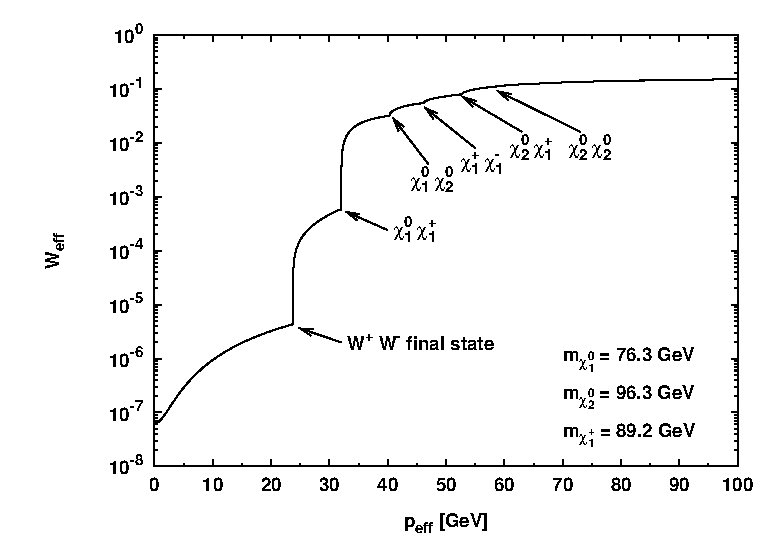
\epsfig{file=fig/rateex.eps,width=0.75\textwidth}}
  \caption{The effective invariant annihiliation rate $W_{\rm eff}$
    as a function of $p_{\rm eff}$ for an example \code{mssm} model. 
    The final state threshold for
    annihilation into $W^+ W^-$ and the coannihilation thresholds, as
    given by Eq.~(\protect\ref{eq:weff}), are indicated.  
    The $\chi_2^0 \chi_2^0$ coannihilation threshold is too small to
    be seen.}
  \label{fig:effrate}
\end{figure}

In the effective annihilation rate, coannihilations appear
as thresholds at $\sqrt{s}$ equal to the sum of the masses of the
coannihilating particles.  We show an example for neutralino
DM (in the \code{mssm} module) in
Fig.~\ref{fig:effrate} where it is clearly seen that the
coannihilation thresholds appear in the effective invariant rate
just as final state thresholds do.  For the same example,
Fig.~\ref{fig:k1effrate} shows the differential annihilation rate
per unit volume $dA/dp_{\rm eff}$, the integrand in
Eq.~(\ref{eq:Apeff}), as a function of $p_{\rm eff}$. We have
chosen a temperature $T=m_{\chi}/20$, a typical freeze-out
temperature. The Boltzmann suppression contained in the exponential
decay of $K_{1}$ at high $p_{\rm eff}$ is clearly visible.  At
higher temperatures the peak shifts to the right and at lower
temperatures to the left.  For the particular model shown in
Figs.~\ref{fig:effrate}--\ref{fig:k1effrate}, the relic density
results $\Omega_\chi h^2=0.030$ when coannihilations are included
and $\Omega_\chi h^2=0.18$ when they are not. Coannihilations
have lowered $\Omega_\chi h^2$ by a factor of 6.

\begin{figure}
  \centerline{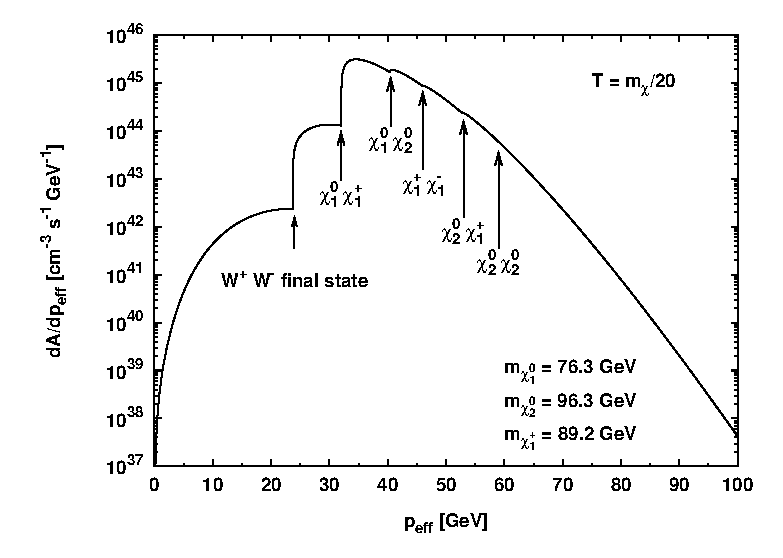
\epsfig{file=fig/k1rateex.eps,width=0.75\textwidth}}
  \caption{Total differential annihilation rate per unit volume 
    $dA/dp_{\rm eff}$ for the same model as in
    Fig.~\protect\ref{fig:effrate}, evaluated at a temperature
    $T=m_\chi/20$, typical of freeze-out. Notice the Boltzmann
    suppression at high $p_{\rm eff}$.}
  \label{fig:k1effrate}
\end{figure}



%%%%%%%%%%%%%%%%%%%%%%%%%%%%%%%%%%%%%%
\subsection{Reformulation of the Boltzmann equation}

%\index{Boltzmann equation}
We now follow Gondolo and Gelmini \cite{Gondolo:1990dk} to 
put Eq.~(\ref{eq:Boltzmann2}) in a more convenient form by
considering the ratio of the number density to the entropy density,
\begin{equation} \label{eq:ydef}
  Y = \frac{n}{s}.
\end{equation}
Consider
\begin{equation}
  \frac{dY}{dt} = \frac{d}{dt} \left( \frac{n}{s} \right) = 
  \frac{\dot{n}}{s}-\frac{n}{s^2}\dot{s}
\end{equation}
where dot means time derivative. In absence
of entropy production, $S=R^3s$ is constant ($R$ is the scale factor).
Differentiating with respect to time we see 
that
\begin{equation}
  \dot{s} = -3\frac{\dot{R}}{R} s = -3Hs
\label{eq:entropycons}
\end{equation}
which yields
\begin{equation}
  \dot{Y} = \frac{\dot{n}}{s} + 3H \frac{n}{s}.
\end{equation}
Hence we can rewrite Eq.~(\ref{eq:Boltzmann2}) as
\begin{equation} \label{eq:Boltzmann3}
  \dot{Y} = -s  \langle \sigma_{\rm{eff}} v \rangle 
  \left( Y^2 - Y_{\rm{eq}}^2 \right).
\end{equation}

The right-hand side depends only on temperature, and it is therefore
convenient to use temperature $T$ instead of time $t$ as independent
variable. Defining $x=m_1/T$ we have
\begin{equation}
  \frac{dY}{dx} = - \frac{m_{1}}{x^2} \frac{1}{3H} \frac{ds}{dT}
  \langle \sigma_{\rm{eff}} v \rangle \left( Y^2 -
  Y_{\rm{eq}}^2 \right).
\label{eq:Boltzmann3bis}
\end{equation}
where we have used
\begin{equation}
  \frac{1}{\dot{T}} = \frac{1}{\dot{s}} \frac{ds}{dT} = -
  \frac{1}{3Hs} \frac{ds}{dT} 
\end{equation} 
which follows from Eq.~(\ref{eq:entropycons}). 
With the Friedmann equation in a radiation dominated universe
\begin{equation}
  H^2 = \frac{8\pi G \rho}{3} ,
\end{equation}
where $G$ is the gravitational constant, and the
usual parameterization of the energy and entropy densities
in terms of the effective degrees of freedom $g_{\rm{eff}}$ and
$h_{\rm{eff}}$, \begin{equation} \label{eq:geffheff}
  \rho = g_{\rm{eff}}(T) \frac{\pi^2}{30} T^4
  , \quad 
  s = h_{\rm{eff}}(T) \frac{2\pi^2}{45} T^3 ,
\end{equation}
we can cast Eq.~(\ref{eq:Boltzmann3bis})
into the form \cite{Gondolo:1990dk}
\begin{equation} \label{eq:Boltzmann4}
  \frac{dY}{dx} = - \sqrt{\frac{\pi}{45G}} \frac{g_{*}^{1/2}m_1}{x^2}
  \langle \sigma_{\rm{eff}} v \rangle \left( Y^2 -
  Y_{\rm{eq}}^2 \right) 
\end{equation}
where $Y_{\rm eq}$ can be written as
\begin{equation}
  Y_{\rm{eq}} = \frac{n_{\rm{eq}}}{s} = 
  \frac{45 x^2}{4 \pi^4 h_{\rm{eff}}(T)} \sum_i g_i
  \left( \frac{m_i}{m_1} \right)^2 K_{2} \left( x 
\frac{m_{i}}{m_1}\right),
\end{equation}
using Eqs.~(\ref{eq:neq}), (\ref{eq:ydef}) and
(\ref{eq:geffheff}).

The parameter $g_{*}^{1/2}$ is defined as
\begin{equation}
  g_{*}^{1/2} = \frac{h_{\rm{eff}}}{\sqrt{g_{\rm{eff}}}}
  \left( 1+\frac{T}{3h_{\rm{eff}}} \frac{d h_{\rm{eff}}}{dT}
  \right)
\end{equation}

For $g_{\rm eff}$, $h_{\rm eff}$ and $g_*^{1/2}$, the user can choose different implementations by a call to 
the routine \code{dsrdset} (see that routine for further details). The default for those effective relativistic 
degrees of freedom is to use the results from Drees et al \cite{Drees:2015exa}.

%Our results are insensitive to the
%value of $T_{QCD}$, because due to a lower limit on the neutralino
%mass the neutralino freeze-out temperature is always much larger
%than $T_{QCD}$.

To obtain the relic density we integrate Eq.~(\ref{eq:Boltzmann4})
from $x=0$ to $x_0=m_\chi/T_0$ where $T_0$ is the photon temperature
of the Universe today. The relic density today in units of the
critical density is then given by
\begin{equation}
  \Omega_\chi = \rho_\chi^0/\rho_{\rm
  crit}=m_\chi s_0 Y_0/\rho_{\rm crit}
\end{equation}
where $\rho_{\rm crit}=3 H^2/8 \pi G$ is the critical density, $s_{0}$ 
is the entropy density today and $Y_{0}$ is the result of the 
integration of Eq.~(\ref{eq:Boltzmann4}). With a
background radiation temperature of $T_0=2.726$ K we finally obtain
\begin{equation} \label{eq:omegah2}
  \Omega_\chi h^2 = 2.755\times 10^8 \frac{m_\chi}{\mbox{GeV}} Y_0.
\end{equation}
%%%%% APPENDIX: Relic density - numerical details %%%%%

\section{Relic density -- numerical integration of the density equation}
\label{sec:numdens}

Let us write the evolution equation for the density,
\begin{equation} \label{eq:Boltzmann4}
  \frac{dY}{dx} = - \sqrt{\frac{\pi}{45G}} \frac{g_{*}^{1/2}m_1}{x^2}
  \langle \sigma_{\rm{eff}} v \rangle \left( Y^2 -
  Y_{\rm{eq}}^2 \right) 
\end{equation}
as
\begin{equation} 
  \frac{dY}{dx} = \lambda (Y^2 - q^2),
  \label{eq:evol}
\end{equation}
where $\lambda$ contains the annihilation rate and $q$ represents the
thermal-equilibrium density.

This equation is stiff and an explicit method, like Euler or Runge-Kutta, fails
to converge. To obtain a numerical solution, we use an adaptive implicit
trapezoidal method which we explain in the following.  Basically we discretize
the equation first with a trapezoidal then with an Euler method, and adapt the
step size according to the difference in the updated function values.

For simplicity we denote the right hand wide of eq.~(\ref{eq:evol}) as $f(x)$.
We further write $f_{i} = f(x_i)$ and similarly for the other functions
$\lambda(x)$ and $q(x)$. Given $Y_{i} = Y(x_i)$ we find $Y_{i+1} = Y(x_{i+1}) $
with $x_{i+1} = x_{i} + h$ as follows.

First we discretize the evolution equation as
\begin{equation}
  Y_{i+1} - Y_{i} = h \frac{ f_i + f_{i+1}}{2} .
\end{equation}
We insert
\begin{eqnarray}
  f_{i} &=& \lambda_{i} \left( Y_{i}^2 - q_{i}^2 \right), \\
  f_{i+1} &=& \lambda_{i+1} \left( Y_{i+1}^2 - q_{i+1}^2 \right) ,
\end{eqnarray}
and solve the resulting quadratic equation for $Y_{i+1}$ to obtain
\begin{equation}
  \label{eq:y_one}
  Y_{i+1} = \frac{c}{1+\sqrt{1+uc}} ,
\end{equation}
where
\begin{eqnarray}
c &=& 2 Y_{i} + u \left[ (q^2_{i+1} + \rho q^2_{i}) - \rho Y^2_{i} \right] , \\
u &=& h \lambda_{i+1} ,\\
\rho &=& \lambda_i / \lambda_{i+1} .
\end{eqnarray}
In the expression for $c$ we have explicitly indicated the order of evaluation
which we found avoids round-off errors. If in eq.~(\ref{eq:y_one}) $1+uc$ is
negative, we simply reduce the step $h$ to $h/2$ and try again.


Secondly we discretize the evolution equation as
\begin{equation}
  Y_{i+1} - Y_{i} = h f_{i+1} .
\end{equation}
We insert the expression for $f_{i+1}$ 
and solve the quadratic equation for $Y_{i+1}$ to obtain
\begin{equation}
  \label{eq:y_two}
  Y'_{i+1} = \frac{1}{2} \, \frac{c'}{1+\sqrt{1+uc'}} ,
\end{equation}
where
\begin{equation}
  c' = 4 \left( Y_{i} + u q^2_{i+1} \right) .
\end{equation}
Again if in eq.~(\ref{eq:y_two}) $1+uc'<0$, we reduce the step $h$ to $h/2$ and
try again.

We then adapt the step size according to the relative difference of $Y_{i+1} $
and $Y'_{i+1}$,
\begin{equation}
d = \left| \frac{ Y_{i+1} - Y'_{i+1} }{ Y_{i+1} } \right| .
\end{equation}
If the difference is larger than a prefixed $\epsilon$, set at 0.01, we reduce
the step size $h$ to $hs/\sqrt{\epsilon}$ but never to less than $h/10$.  $s$
is a safety factor set to 0.9. If $d<\epsilon$, we increase the step size by a
factor $s/\sqrt{\epsilon}$ but never by more than a factor of 5.  We do not
allow the step size to become smaller than $h_{\rm min} = 10^{-9}$. Error code
5 is reported if this happens.  Error code 4 occurs when $x_{i+1}$ is
numerically equal to $x_{i}$ because of round-off. Error code 6 occurs when the
number of steps exceeds a maximum of 100000.  Finally the initial step size is
taken to be 0.01.

%%%%%%%%%%%%%%%%%%%%%%%%%%%%%%%%%%%%%%%%%%%%%%%%%%%%%%%%%%%%%%%%%%%%
\section{Relic density -- routines}

In \ft{src/rd}, the general relic density routines are found. These
routines can be used for any dark matter candidate and e.g.\ the interface
to neutralino dark matter is in \ft{src\_models/mssm/rd}. 

The main routine for relic density calculations is \ft{dsrdomega}. It calculates and returns the relic density as well as the approximate temperature of freeze-out. It taks a few arguments: i) one \code{option} argument that typically (depending on the particle physics module) determines how co-annihilations are included, ii) one \code{fast} argument that determines how careful the Boltzmann solver should be in calculating the relic density. See the header of \ft{dsrdomega} for more details.
%\index{relic density}


%%%%%%%%%%%%%%%%%%%%%%%%%%%%%%%%%%%%%%%%%%%%%%%%%%
\subsection{Global parameters}

All internal settings of the relic density routines are set in common
blocks in \ft{dsrdcom.h}. The most important parameters that can be
changed by the user are

\begin{sub}{Important parameters in \ftb{dsrdcom.h}}
  \itit{Purpose:} Provide a set of parameters, with which the internal
  behaviour of the relic density routines can be changed.
  \itit{Parameters}
  \itv{tharsi}{i} Size of the coannihilation, resonance and threshold
    arrays (default=50). Increase this size if you have more than 50
    coannihilating particles, more than 50 resonances or more than 50
    thresholds.
  \itv{rdluerr}{i} Logical unit number where error messages are
    printed.
  \itv{rdtag}{c*12} Idtag that is printed in case of errors.
  \itv{cosmin}{r8} \ldots
  \itv{waccd}{r8} \ldots
  \itv{dpminr}{r8} \ldots
  \itv{dpthr}{r8} \ldots
  \itv{wdiffr}{r8} \ldots
  \itv{wdifft}{r8} \ldots
  \itv{hstep}{r8} \ldots
  \itv{rdt\_max}{r8} Maximum number of seconds to spend on relic density calculation. If the time limit is exceeded, \ft{dsrdomega} returns with an error flag and the result 0. The time is the total CPU time (i.e.\ summed up over all cores/threads) and the limit is approximate as it is only checked before a new point is added to the $W_{\rm eff}$ tabulation.
\end{sub}


%%%%%%%%%%%%%%%%%%%%%%%%%%%%%%%%%%%%%%%%%%%%%%%%%%
\subsection{Brief description of the internal routines}

Below, the remaining routines related to the relic density calculation
are briefly mentioned. For more details, we refer to the routines
themselves.

\begin{brief-subs}
\bsub{dsrdaddpt}
  To add one point in the $W_{\rm eff}$-$p_{\rm eff}$ table.
\bsub{dsrdcom}
  To initialize parameters in the common blocks in \ft{dsrdcom.h}. If
  you want to change these parameters yourself, include \ft{dsrdcom.h}
  in your code and change the parameters you want.
\bsub{dsrddof}
  Returns the degrees of freedom as a
  function of the temperature in the early Universe.
\bsub{dsrddpmin}
  To return the allowed minimal distance in $p_{\rm
  eff}$ between two points in the $W_{\rm eff}$-$p_{\rm eff}$ plane.
  The returned value depends on if there is a resonance present or not
  at the given $p_{\rm eff}$.
\bsub{dsrdens} Routine to solve the Boltzmann equation and return the relic density. Called by \ft{dsrdomega}.
\bsub{dsrdeqn}
  To solve the relic density equation by means of an
  implicit trapezoidal method with adaptive stepsize and termination.
\bsub{dsrdfunc}
  To return the invariant annihilation rate times the
  thermal distribution.
\bsub{dsrdfuncs}
  To provide \ft{dsrdfunc} in a form suitable for
  numerical integration.
\bsub{dsrdlny}
  To return $\ln W_{\rm eff}$ for a given $p_{\rm
  eff}$.
\bsub{dsrdnormlz}
  To return a unit vector in a given direction.
\bsub{dsrdqad}
  To calculate the relic density with a
  quick-and-dirty method. It uses the approximative expressions in
  Kolb \& Turner with the cross section expaned in $v$.
\bsub{dsrdqrkck}
  To numerically integrate a function with a
  Runge-Kutta method
\bsub{dsrdrhs}
  To calculate terms on the right-hand side in the
  Boltzmann equation.
\bsub{dsrdset}
  To set the control parameters for the relic density calculation. Currently, only the choice of effective degrees of freedom is implemented through \ft{dsrdset}; the other parameters are passed as arguments to \ft{dsrdomega}.
\bsub{dsrdspline}
  To set up the table $W_{\rm eff}$-$p_{\rm eff}$ for
  spline interpolation.
\bsub{dsrdstart}
  To sort and store information about coannihilations,
  resonances and thresholds in common blocks.
\bsub{dsrdtab}
  To set up the table $W_{\rm eff}$-$p_{\rm eff}$.
\bsub{dsrdthav}
  To calculate the thermally averaged annihilation
  cross section at a given temperature.
\bsub{dsrdthclose}
  ...
\bsub{dsrdthlim}
  To determine the end-points for the thermal
  average integration.
\bsub{dsrdthtest}
  To check if a given entry in the $W_{\rm
  eff}$-$p_{\rm eff}$ table is at a threshold.
%\bsub{dsrdwdwdcos}
%  To write out a table of $dW_{\rm eff}/d\cos \theta$
%  as a function of $\cos \theta$ for a given $p_{\rm eff}$.
\bsub{dsrdwfunc}
  To write out \ft{dsrdfunc} for a given $x=m_\chi/T$.
\bsub{dsrdwintp}
  To return the invariant rate $W_{\rm eff}$ for any
  given $p_{\rm eff}$ by performing a spline interpolation in the
  $W_{\rm eff}$-$p_{\rm eff}$ table.
\bsub{dsrdwintpch}
  To check the spline interpolation in the $W_{\rm
  eff}$-$p_{\rm eff}$ table and compare with a linear interpolation.
\bsub{dsrdwintrp}
  To write out a table of the invariant rate $W_{\rm
  eff}$ and some internal integration variables and expressions.
\bsub{dsrdwres}
  To write out the table $W_{\rm eff}$-$p_{\rm eff}$.
\end{brief-subs}

\chapter[se\_aux: Auxiliary routines for WIMP annihilation in the Sun/Earth]{\codeb{se\_aux}:\\ Auxiliary routines for WIMP annihilation in the Sun/Earth}
\label{ch:src/se_aux}

%%%%%%%%%%%%%%%%%%%%%%%%%%%%%%%%%%%%%%%%%%%%%%%%%%%%%%%%%%%%%%%%%%%%%%
\section{Sun and Earth models -- auxiliary routines}

This directory contains parameterizations and semi-analytical calculations of auxiliary fluxes, like Earth atmospheric fluxes. They are not up to date with the latest calculations and are provided as is for convenience.

\chapter[se\_mod: Sun and Earth models]{\codeb{se\_mod}:\\ Sun and Earth models}
\label{ch:src/se_mod}

\joakim{I am responsible for updating this part}
%%%%%%%%%%%%%%%%%%%%%%%%%%%%%%%%%%%%%%%%%%%%%%%%%%%%%%%%%%%%%%%%%%%%%%
\section{Sun and Earth models -- theory}


We need to have accurate models for the Sun and the Earth, both in terms of mass distributions, but also in terms chemical compositions etc. We here include
a set of Sun and Earth models.

The models here are used for the capture rate calculation for capture of WIMPs in the Sun and the Earth, but they are also used for external packages like \ftb{WimpSim} which simulates neutrino interactions and oscillations on the way out of the Sun/Earth. Those simulation results are included as tables in \texttt{se\_yield}.
 %%%%%%%%%%%%%%%%%%%%%%%%%%%%%%%%%%%%%%%%%%%%%%%%%%%%%%%%%%%%%%%%%%%%%%
\section{Sun and Earth models -- routines}

The main routines that could be of interest to most users are


\chapter[se\_nu: Capture and annihilation in the Sun/Earth]{\codeb{se\_nu}:\\ Capture and annihilation in the Sun/Earth}
\label{ch:src/se_nu}

%%%%%%%%%%%%%%%%%%%%%%%%%%%%%%
%%%%%%%%%%%%%%%%%%%%%%%%%%%%%%
\section{Neutrinos from the Sun and Earth --  theory}

\comment{Update this section.}

{\bfseries. Note. This chapter is not up to date with the latest additions to the code, but provided as is as a reference right now.}

There are several indirect methods for detection of WIMPs.
One of the most promising \cite{Krauss:1985unpub,Press:1985ug,Silk:1985ax,Krauss:1985ks,Krauss:1985aaa,Gaisser:1986ha,Griest:1986yu,Hagelin:1986gv,Freese:1985qw,Kamionkowski:1991nj,Halzen:1991kh,Bottino:1991dy,Bottino:1994xp,Gandhi:1993ce,Bergstrom:1996kp,Bergstrom:1998xh} is to make use of the
fact that scattering of halo neutralinos by the Sun and the planets,
in particular the Earth, during the several
billion years that the Solar system has existed, will have trapped
these neutralinos within these astrophysical bodies. Being trapped
within the Solar or terrestrial material, they will sink towards
the center, where a considerable enrichment and corresponding
increase of annihilation rate will occur.


Searches for neutralino annihilation into neutrinos
will be subject to  extensive experimental investigations in view
of the new neutrino telescopes (AMANDA, IceCube, Baikal, NESTOR, ANTARES)
planned or under construction \cite{Halzen:1996su}. A high-energy
neutrino signal in the direction of the centre of the Sun or Earth
is an excellent experimental signature which may stand up against
the background of neutrinos generated by cosmic-ray interactions in the
Earth's atmosphere.

There are several different approximations one could do, or processes to
include when calculating the capture rates in the Earth/Sun and many of these
are coded into \ds. The default in \ds\ is always to use the best calculations
available, but more approximate (older) routines are also available,
as well as more speculative signals, like the Damour-Krauss signal
(not included by default). If you want to use something else than the
defaults, or want to call more internal rotuines (more internal than
\code{dsntrates} or \code{dsntdiffrates}), you should read the
following sections carefully.


%%%%%%%%%%%%%%%%%%%%
\subsection{Neutrino yield from annihilations}

The differential neutrino flux from neutralino annihilation is
\beq
\frac{dN_\nu}{dE_\nu} =
\frac{\Gamma_A}{4\pi D^2} \sum_{f}
B^{f}_{\chi}\frac{dN^f_\nu}{dE_\nu}
\eeq
where $\Gamma_A$ is the annihilation rate,
$D$ is the distance of the detector from the source (the
central region of the Earth or the Sun), $f$ is the neutralino pair
annihilation final states,
and $B^{f}_{\chi}$ are the branching ratios into the final state $f$.
  $dN^f_\nu/dE_{\nu}$ are the energy
distributions of  neutrinos generated by the final state $f$ and are
obtained from the {\sc Pythia} simulations described in section
\ref{sec:mcsim}. \joakim{Update reference and description of WimpSim simulations.}

In comparison with calculations using the results of \cite{Ritz:1987mh}
(e.g.\ ~\cite{Giudice:1988vs,Halzen:1991kh,Drees:1993bh,Gandhi:1993ce,Bottino:1994xp,Jungman:1994jr,Berezinsky:1996ga}), this
Monte Carlo treatment of the neutrino propagation through the Sun
does not need the simplifying assumptions previously made, namely neutral
currents are no more assumed to be much weaker than charged currents
and energy loss is no more considered continuous.

The neutrino-induced muon flux may be detected in a neutrino telescope
by measuring the muons that come from the direction of the centre
of the Sun or Earth. For a shallow detector, this usually has to
be done in the case of the Sun by looking (as always the case for
the Earth) at upward-going muons, since there is a huge background
of downward-going muons created by cosmic-ray interactions in the
atmosphere. There is always in addition a more isotropic
background coming from muon neutrinos created on the other side of
the Earth in such cosmic-ray events (and also from cosmic-ray
interactions in the outer regions of the Sun).
The flux of muons at the detector is  given by

\beq
\frac{d N_\mu}{d E_\mu}
= N_A \int^\infty_{E_\mu^{\rm th}} d E_\nu
\int_0^\infty d\lambda \int_{E_\mu}^{E_\nu}
d {E'_\mu }\,\,
P(E_\mu,E'_\mu; \lambda)\,\,
\frac{d \sigma_\nu (E_\nu,E'_\mu)}{d E'_\mu} \,\,
\frac{d N_\nu}{d E_\nu}\, ,
\label{eq:muflux}
\eeq
where $\lambda$ is the muon range in the medium (ice or water
for the large detectors in the ocean or at the South Pole,
or rock which surrounds the smaller underground detectors),
$d \sigma_\nu (E_\nu,E'_\mu) / d E'_\mu$ is
the weak interaction cross section for production of a muon of
energy $E'_\mu$ from a parent neutrino of energy $E_\nu$, and
$P(E_\mu,E'_\mu; \lambda)$ is the
probability for a muon of initial energy $E'_\mu$
to have a final energy $E_\mu$ after passing
  a path--length $\lambda$ inside the detector medium.
$E_\mu^{\rm th}$ is the detector threshold energy, which for
``small''
neutrino telescopes like Baksan, MACRO and Super-Kamiokande is
around 1 GeV.
Large area neutrino telescopes in the ocean  or in Antarctic ice
typically
have thresholds of the order of tens of GeV, which makes them
sensitive mainly to heavy neutralinos (above 100 GeV)
\cite{Bergstrom:1998xh}.

The integrand in Eq.~(\ref{eq:muflux}) is weighted towards high
neutrino energies, both because the cross section $\sigma_\nu$
rises approximately linearly with energy and because the average
muon energy, and therefore the range $\lambda$, also grow
approximately linearly with $E_\nu$. Therefore, final states
which give a hard neutrino spectrum (such as heavy quarks, $\tau$
leptons and $W$ or $Z$ bosons) are usually more important
than the soft spectrum arising from light quarks and gluons.

%%%%%%%%%%%%%%%%%%%%
\subsection{Evolution of the number density in the Earth/Sun}

Neutralinos are steadily being trapped in the Sun or Earth by
scattering, whereas annihilations take them away.
Let $N(t)$ be the total number of neutralinos trapped, at time $t$, in the core
of, for example,  the Earth.
The annihilation rate of neutralino pairs can be written as
\begin{equation}
\Gamma_a (t) = \frac{1}{2} \ C_a \, N^2 (t) \, . \label{eqx.1}
\end{equation}

The evolution of $N(t)$ is the result of the competition between capture and
annihilation:
\begin{equation}
\frac{dN}{dt} = C_c (t) - C_a \, N^2 \label{eqx.2}
\end{equation}
The constant $C_c$ is the capture rate, and
$C_a$ entering equations (\ref{eqx.1}) and (\ref{eqx.2}) is linked to
the annihilation cross-section $\sigma_a$, and to some effective volumes $V_j$,
$j=1,2$, taking into account the quasi-thermal distribution of neutralinos in
the Earth core:
\begin{equation}
C_a = \langle \sigma_a \, v \rangle \, \frac{V_2 }{ V_1^2} \, , \label{eq6.3}
\end{equation}
\begin{equation}
V_j \simeq 2.3 \times 10^{25} \, \left(\frac{j \, m_X}{ 10 \, {\rm 
GeV}}\right)^{-3/2} \, {\rm
cm}^3 \, . \label{eq6.4}
\end{equation}

This has the solution for the annihilation rate implemented in \ds\
\beq
\Gamma_A={C_c\over 2} \tanh^2\left({t\over \tau}\right),\label{eq:tanh}
\eeq
where the equilibration time scale $\tau=1/\sqrt{C_cC_a}$.  In most
cases for the Sun, and in the cases of observable fluxes for the
Earth, $\tau$ is much smaller than a few billion years, and therefore
equilibrium is often a good approximation ($\dot N(t)=0$).
This means
that it is the capture rate which is the important quantity that
determines the neutrino flux. However, in the program we keep the exact
formula (\ref{eq:tanh}), with some
modifications discussed in Sec.~\ref{sec:dk}).

%%%%%%%%%%%%%%%%%%%%
\subsection{Approximate capture rate expressions}

The capture rate induced by scalar (spin-independent) interactions
between the neutralinos and the nuclei in the interior of the Earth or
Sun is the most difficult one to compute, since it depends sensitively
on the Higgs mass, form factors, and other poorly known quantities.
However, this spin-independent capture rate calculation is the same as
for direct detection treated in Chapter~\ref{ch:src/dd}.  Therefore,
there is a strong correlation between the neutrino flux expected from
the Earth (which is mainly composed of spin-less nuclei) and the
signal predicted in direct detection experiments \cite{Bergstrom:1998xh,Kamionkowski:1994dp}.
It seems that even the large (kilometer-scale) neutrino telescopes
planned, when searching for neutralino annihilation in the Earth, will
not be competitive with the next generation of direct detection
experiments when it comes to detecting neutralino dark matter.
However, the situation concerning the Sun is more favourable.  Due to
the low counting rates for the spin-dependent interactions in
terrestrial detectors, high-energy neutrinos from the Sun constitute a
competitive and complementary neutralino dark matter search.  Of
course, even if a neutralino is found through direct detection, it
will be extremely important to confirm its identity and investigate
its properties through indirect detection.  In particular, the mass
can be determined with reasonable accuracy by looking at the angular
distribution of the detected muons \cite{Edsjo:1995zc,Bergstrom:1997tp}.

For the Sun, dominated by hydrogen, the axial (spin-dependent)
cross section is important and relatively easy to compute.  A
reasonably good
approximation is given by \cite{Jungman:1995df}
\beq
      {C^{\rm sd}_\odot\over (1.3\cdot 10^{23}\, {\rm s}^{-1})
\left(270\ {\rm km\,s^{-1}}/ \bar v\right)}=
\left({\rho_\chi\over 0.3\ {\rm GeV}\,{\rm cm}^{-3}}\right)
      \left({100\,{\rm GeV}\over m_\chi}\right)
\left({\sigma_{p\chi}^{\rm sd}\over 10^{-40}\ {\rm
      cm}^2}\right)
\eeq
where $\sigma_{p\chi}^{\rm sd}$ is the cross section for
neutralino-proton elastic scattering via the axial-vector interaction,
$\bar v$ is the dark-matter velocity dispersion, and $\rho_\chi$ is
the local dark matter mass.  The capture rate in the Earth is
dominated by scalar interactions, where there may be kinematic and
other enhancements, in particular if the mass of the neutralino almost
matches one of the heavy elements in the Earth.  For this case, a more
detailed analysis is called for, which is available in \cite{Gould:1987ir}
with convenient approximations in \cite{Jungman:1995df}.
   In fact, also for the
Sun the spin-independent contribution can be important, in particular
iron may contribute non-negligibly.
For the Sun, the
  approximation in \cite{Jungman:1995df} is also available,
\beqa
      {C^{\rm si}_\odot\over (4.8\cdot 10^{22}\, {\rm s}^{-1})
\left(270\ {\rm km\,s^{-1}}/ \bar v\right)}=
\left({\rho_\chi\over 0.3\ {\rm GeV}\,{\rm cm}^{-3}}\right)
      \left({100\,{\rm GeV}\over m_\chi}\right)\times & &\nonumber\\
\sum_A\left({\sigma_{A}^{\rm si}\over 10^{-40}\ {\rm
      cm}^2}\right)F_A(m_\chi)f_A\phi_AS\left(m_\chi/m_{A}\right)/m_{A},
\eeqa
where $f_A$ is the mass fraction of element $A$ and $\phi_A$ is the
typical gravitational potential (relative to the surface) for that
element. I.e.\ an element that is concentrated in the core will have a
higher $\phi_A$ than an element at the surface. $A$ is the atomic
number of the element and $M_{A}$ is its mass. The factor $S$ is a
kinematical suppression factor \cite{Jungman:1995df,Kamionkowski:1991nj}. In the next
subsection we will go through the compositions of the Earth/Sun that
we use.

The approximate capture rate expressions above are coded into the routines
\code{dsntcapsun} and \code{dsntcapearth}. More accurate expressions
will follow in the coming subsections.


%%%%%%%%%%%%%%%%%%%%%%%%%%%%%%
\subsection{Earth and Sun composition}

When the capture rates are calculated, we need to know the composition
and density of the Earth/Sun as a function of depth.  

In \cite{Jungman:1995df} they used average mass fractions and potentials for the
location of the various elements in the Sun. We have updated these to
the BP2000 \cite{Bahcall:2000nu} values instead, as given in Table~\ref{tab:suncomp}

\begin{table}
  \centering
  \begin{tabular}{lccc}
   & & \multicolumn{2}{c}{Average parameters} \\ \cline{3-4}
   Element & Mass number ($A$) & $f_i$ & $\phi_i$ \\ \hline
   Hydrogen, H       &  1 & 0.670    & 3.15 \\
   Helium-4, $^4$He  &  4 & 0.311    & 3.40 \\
   Carbon, C         & 12 & 0.00237  & 2.85 \\
   Nitrogen, N       & 14 & 0.00188  & 3.83 \\
   Oxygen, O         & 16 & 0.00878  & 3.25 \\
   Neon, Ne          & 20 & 0.00193  & 3.22 \\
   Magnesium, Mg     & 24 & 0.000733 & 3.22 \\
   Silicon, Si       & 28 & 0.000798 & 3.22 \\
   Sulphur, S        & 32 & 0.000550 & 3.22 \\
   Iron, Fe          & 56 & 0.00142  & 3.22 \\ \hline
\end{tabular}
\caption{The composition of the Sun with average parameters to be used
  in the approximative relations given in \cite{Jungman:1995df}. These values are
  updated with the solar model of \cite{Bahcall:2000nu} and differs slightly
  from the values used in \cite{Jungman:1995df}.}
  \label{tab:suncomp}
\end{table}

\begin{table}
  \centering 
  \begin{tabular}{lcccccc}
& Mass & \multicolumn{2}{c}{Mass fraction} & & \multicolumn{2}{c}{Average parameters}
\\ \cline{3-4} \cline{6-7}
 Element & number ($A$) & Core & Mantle & & $f_i$ & $\phi_i$ \\ \hline
  Oxygen, O     & 16 & 0.0   & 0.440   & & 0.298   & 1.20  \\
  Silicon, Si   & 28 & 0.06  & 0.210   & & 0.162   & 1.24  \\
  Magnesium, Mg & 24 & 0.0   & 0.228   & & 0.154   & 1.20  \\
  Iron, Fe      & 56 & 0.855 & 0.0626  & & 0.319   & 1.546 \\
  Calcium, Ca   & 40 & 0.0   & 0.0253  & & 0.0171  & 1.20  \\
  Phosphor, P   & 30 & 0.002 & 0.00009 & & 0.00071 & 1.56  \\
  Sodium, Na    & 23 & 0.0   & 0.0027  & & 0.00183 & 1.20  \\
  Sulphur, S    & 32 & 0.019 & 0.00025 & & 0.0063  & 1.59  \\
  Nickel, Ni    & 59 & 0.052 & 0.00196 & & 0.0181  & 1.57  \\
  Aluminum, Al  & 27 & 0.0   & 0.0235  & & 0.0159  & 1.20  \\
  Chromium, Cr  & 52 & 0.009 & 0.0026  & & 0.0047  & 1.44  \\ \hline
\end{tabular}
  \caption{The composition of the Earth's core and mantle. The core
    mass fractions are from \cite{2003TrGeo...2..547M}[Table 4] and the mantle
    mass fractions are from \cite{2003TrGeo...2..547M}[Table 2]. The average
    mass fractions and potentials in the last two columns are weighted
    averages assuming a core mass of $1.93\cdot10^{24}$ kg and a
    mantle mass of $4.04\cdot10^{24}$ kg with average potentials
    (relative to the surface) of 1.6 in the core and 1.2 in the mantle
    \cite{Gould:1987ir}.} \label{tab:earthcomp} 
\end{table}

For the Earth, we have also implemented more accurate
density profiles and more up-to date chemical distributions within the
Earth. We use the estimates for the Earth composition given in
\cite{2003TrGeo...2..547M}[Table 2 for the mantle and Table 4 for the core]. In
Table~\ref{tab:earthcomp} we list these values together with the
average parameters $f_i$ and $\phi_i$ that should be used in the
expressions for the approximate capture rates in the previous
section. Note that using these average parameters instead of
integrating over the full radius is equivalent to putting all the
elements of the give type at the gravitational potential $\phi_i$.

\begin{figure}
\centerline{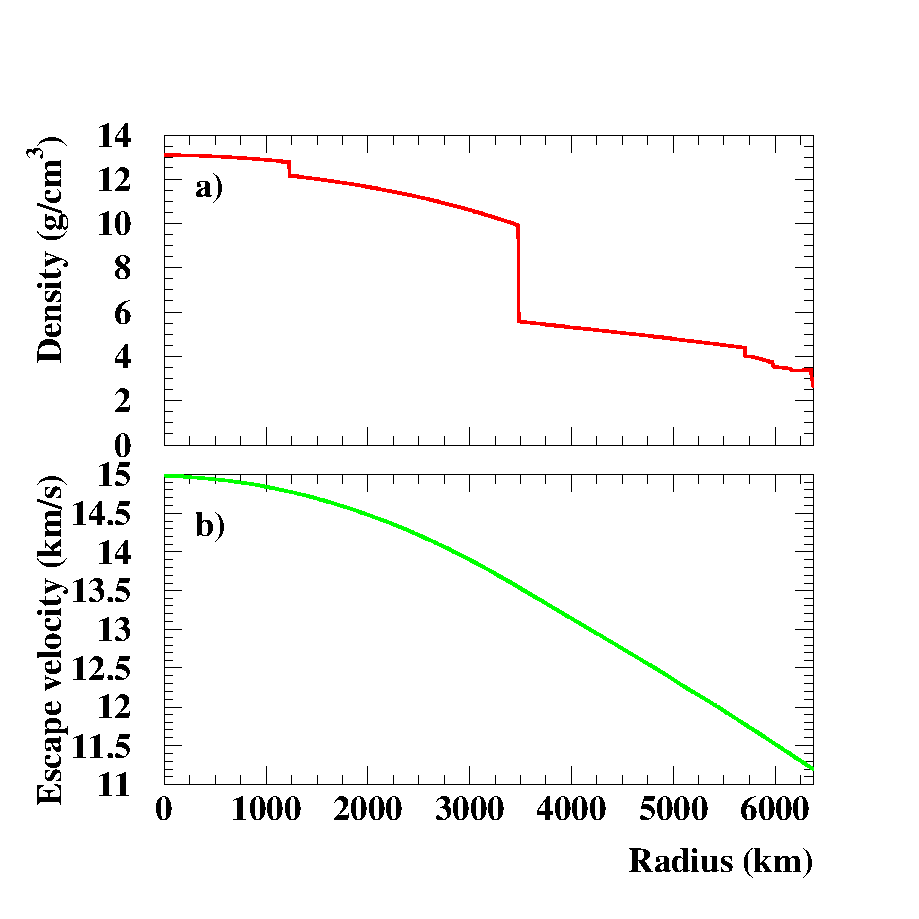
\epsfig{file=fig/eadensvesc.eps,width=0.6\textwidth}}
\caption{In a) the density profile and in b) the escape velocity in the Earth is shown.}
\label{fig:eadensvesc}
\end{figure}

We also need the density profile of the Earth, and for this we use the
values in \cite{EncBrit}. Using this density profile, we can calculate
the gravitational potential, $\phi(r)$ inside the Earth and from this
one the escape velocity $v$ inside the Earth,
\begin{equation}
   \label{eq:vesc}
   v = 11.2 \sqrt{\frac{\phi(r)}{\phi(R_\oplus)}} \mbox{~km/s.}
\end{equation}
In Fig.~\ref{fig:eadensvesc} we show the density profile and escape
velocity inside the Earth. 

%%%%%%%%%%%%%%%%%%%%%%%%%%%%%%%%%%%%%%%%
\subsection{More accurate capture rate expressions}

Another complicating factor when calculating the capture rates is the
integration over the velocity 
distribution. In \cite{Gould:1987ir}, parts of the integrations are
performed analytically for a Gaussian veolocity distributions. These
expressions are also coded in \ds for the Earth and give a more
accurate calculation of the capture rate in the Earth than the
approximations given above. The routine \code{dsntcapearth2} performs
these calculations for the Earth.

%%%%%%%%%%%%%%%%%%%%%%%%%%%%%%
\subsection{Accurate capture rates in the Earth for general velocity distributions}


If one wants even more accurate and general expressions for the
capture rates in the Sun/Earth, we have also implemented the full
expressions in \cite{Gould:1987ir}, but without assuming that the velocity
distribution is a Gaussian (or Maxwell-Boltzmann). These routines are
now the default in \ds.

We will here outline how these expressions look
like for the Earth and how they can be used both for a Maxwell-Boltzmann
distribution and for a general velocity distribution. The expressions
will of course look analogously for the Sun. We start with
the general case and study the special case of a Maxwell-Boltzmann
distribution in the next section. 

We will divide the Earth into shells and calculate the capture from
element $i$ in each shell individually. At the end we will integrate
over all the shells and sum over all the elements in the Earth. The
capture rate from element $i$ per unit shell volume is given by
\cite{Gould:1987ir}[Eq.~(2.8)] 
\begin{equation}
\label{eq:dcdv}
    \frac{dC_i}{dV} = \int_0^{u_{max}} du \frac{f(u)}{u} w \Omega_{v,i}^-(w)
\end{equation}
where $f(u)$ is the velocity distribution (normalized such that
$\int_0^\infty\ f(u) = n_\chi$ where $n_\chi$ is the number density of
WIMPs. The expression $\Omega_{v,i}^-(w)$ is related to the
probability that we scatter to orbits below the escape velocity. $w$
is the velocity at the given shell and it is related to the velocity
at infinity $u$ and the escape velocity $v$ by 
\begin{equation}
   w = \sqrt{u^2 + v^2}.
\end{equation}
The upper limit of integration is a priori set to $u_{max} = \infty$,
but we will see below that due to kinematical reasons we can set it to
a lower value (Eq.~(\ref{eq:umax}) below). 
If we allow for a form factor suppression of the form \cite{Gould:1987ir}[Eq.~(A3)]
\begin{equation}
   |F(q^2)|^2 = \exp\left( - \frac{\Delta E}{E_0} \right)
\end{equation}
with \cite{Gould:1987ir}[Eq.~(A4)]
\begin{equation}
   E_0 = \frac{3 \hbar^2}{2m_\chi R^2}
\end{equation}
we can evaluate $w \Omega_{v,i}^-(w)$ and arrive at the expression
\cite{Gould:1987ir}[Eq.~(A6)] 
\begin{equation}
\label{eq:womega}
   w \Omega_{v,i}^- (w) = \sigma_i n_i \frac{\mu_+^2}{\mu}2 E_0 \left[
   e^{- \frac{m_\chi u^2}{2E_0}} - e^{-\frac{\mu}{\mu_+^2}m_\chi \frac{u^2+v^2}{2E_0}}
   \right] \Theta\left( \frac{\mu}{\mu_+^2} - \frac{u^2}{u^2+v^2} \right)
\end{equation}
where we have introduced
\begin{equation}
   \mu = \frac{m_\chi}{m_i} \quad ; \quad \mu_\pm = \frac{\mu \pm 1}{2}
\end{equation}
with $m_i$ the mass of element $i$. The Heaviside step function
$\Theta$ plays the role of only including WIMPs that can scatter to a
velocity lower then the escape velocity $v$. To simplify our
calculations we can drop this step function in Eq.~(\ref{eq:womega})
and instead set the upper limit of integration in Eq.~(\ref{eq:dcdv})
to 
\begin{equation}
\label{eq:umax}
  u_{max} = \sqrt{\frac{\mu}{\mu_-^2}} v
\end{equation}
We also need the scattering cross section on element $i$, which can be
written as 
\cite{Jungman:1995df}[Eq.~(9-25)]
\begin{equation}
\label{eq:sigma_i}
   \sigma_i = \sigma_p A_i^2 \frac{(m_\chi m_i)^2}{(m_\chi+m_i)^2} 
   \frac{(m_\chi + m_p)^2}{(m_\chi m_p)^2}
\end{equation}
where $A_i$ is the atomic number of the element, $m_p$ is the proton
mass and $\sigma_p$ is the scattering cross section on protons. 

We now have what we need to calculate the capture rate. In
Eq.~(\ref{eq:dcdv}) we integrate over the velocity for our chosen
velocity distribution. We then integrate this equation over the radius
of the Earth and sum over all the different elements in the Earth, 
\begin{equation}
   C = \int_0^{R_\oplus} dr \sum_i \frac{dC_i}{dV} 4 \pi r^2
\end{equation}
Note that we have not assumed anything special about our velocity
distribution, it doesn't even have to be isotropic since the
distribution of elements evenly in the shells will make an anisotropic
distribution on average to behave as an isotropic one. 

The routines that calculate the capture rates with these general (and
accurate) expressions are \code{dsntcapearthnum} and
\code{dsntcapsunnum}. As these calculations are somewhat
time-consuming, we have also added a possibility to tabulate the
result and interpolate in these tables. To use (or create, if the
table files are missing) instead call \code{dsntcapearthtab} and
\code{dsntcapsuntab}. These last two routines are the default in
\ds. The velocity distribution used is determined by a switch when the
halo model is set (i.e.\ when \code{dshmset} is called).


%%%%%%%%%%
\subsection{Accurate capture rates for the Earth for a
  Maxwell-Boltzmann velocity distribution}

We will here give some more information on how the approximations
introduced in the beginning of this chapter are derived from the
general expressions in the preceeding section.

If the velocity distribution is of Maxwell-Boltzmann type we can
greatly simplify our expressions above as we can perform the
integration over velocity analytically. The integration over radius
can also be further simplified by using the average mass fractions
$f_i$ and potentials $\phi_i$ in Tables~\ref{tab:suncomp}--\ref{tab:earthcomp}. 

If the velocity distribution in the halo is Maxwell-Boltzmann, it looks like
\begin{equation}
   f_h(u) du = n_\chi \frac{4}{\sqrt{\pi}} \left(\frac{3}{2}\right)^{\frac{3}{2}}
   \frac{u^2}{\bar{v}^3}
   e^{-\frac{3}{2}\frac{u^2}{\bar{v}^2}} du
\end{equation}
where $\bar{v}$ is the three-dimensional velocity dispersion and
$n_\chi$ is the number density of WIMPs in the halo. However, the
solar system moves through the halo with a velocity $v_*$ and the
distribution on observer with this velocity through the halo will see
is 
\begin{equation}
\label{eq:fstaru}
  f_*(u) = f_h(u) e^{-\frac{3}{2}\frac{v_*^2}{\bar{v}^2}} 
  \frac{\sinh\left(\frac{3 u v_*}{\bar{v}^2}\right)}{\frac{3 u v_*}{\bar{v}^2}} =
  n_\chi \sqrt{\frac{3}{2\pi}} \frac{u}{\bar{v} v_*} \left[
  e^{-\frac{3}{2} \frac{( u-v_*)^2}{\bar{v}^2}} -
  e^{-\frac{3}{2} \frac{( u+v_*)^2}{\bar{v}^2}} \right]
\end{equation}
Now one would naively believe that this is not the distribution that
an observer at the Earth will see. First of all, the Earth is moving
with respect to the Sun and secondly, the WIMPs have gained speed by
the gravitational attraction of the Sun when they reach the
Earth. Both of these arguments are true and the distribution of WIMPs
in the halo will not look like Eq.~(\ref{eq:fstaru}) to an observer on
the Earth. However, Gould \cite{Gould:1991aa} showed that WIMPs from the
halo can diffuse into the solar system due to gravitational
interactions with the planets and this distribution of WIMPs will
roughly look like as if the Earth was in free space moving through the
halo with the velocity of the solar system,
i.e.\ Eq.~(\ref{eq:fstaru}). We will later scrutinize this statement,
as it turns out that it does not quite hold, but 
as a first guess it is a reasonable approximation. For the Sun,
though, the velocity distribution give above is the correct one for a
Maxwell-Boltzmann distribution.

With the distribution Eq.~(\ref{eq:fstaru}) we can analytically
perform the integration over velocity in Eq.~(\ref{eq:dcdv}). After
some algebra we arrive at \cite{Gould:1987ir}[Eq.~(A10)] 
\begin{eqnarray}
\frac{dC_i}{dV} & = & \left( \frac{8}{3\pi} \right)^{\frac{1}{2}} 
\frac{\sigma_i n_i n_\chi \bar{v}}{2b\eta} \nonumber \\
 & & \Bigg[ \frac{e^{-a\hat{\eta}^2}}{\sqrt{1+a}} \left[ 2 \widetilde{\rm erf}(\hat{\eta}) - \widetilde{\rm erf} (\hat{A}_+) + \widetilde{\rm erf} (\hat{A}_-) \right]
   \nonumber \\ 
& &  - \frac{e^{-b\check{\eta}^2}}{\sqrt{1+b}}
   e^{-(a-b)A^2} \left[ 2 \widetilde{\rm erf}(\check{\eta}) - \widetilde{\rm erf} (\check{A}_+) + \widetilde{\rm erf} (\check{A}_-)
   \right] \Bigg]
   \label{eq:dcdvmb}
\end{eqnarray}
where $\widetilde{\rm erf}$ is the modified error function,
\begin{equation}
\label{eq:moderf}
   \widetilde{\rm erf} (x) = \frac{\sqrt{\pi}}{2} {\rm erf} (x)
   \qquad ; \qquad {\rm erf}(x) = \frac{2}{\sqrt{\pi}} \int_0^x e^{-y^2} dy.
\end{equation}
Following Gould \cite{Gould:1987ir}, we have in Eq.~(\ref{eq:dcdvmb})
introduced the following shorthand notation: 
\begin{equation}
\begin{array}{ccccc}
\eta = \sqrt{\frac{3}{2}} \frac{v_*^2}{\bar{v}^2} & ; &
a = \frac{m_chi \bar{v}^2}{3E_0} & ; & b=\frac{\mu}{\mu_+^2} a \\
\hat{\eta} = \frac{\eta}{\sqrt{1+a}} & ; & \check{\eta} = \frac{\eta}{\sqrt{1+b}} \\
A^2 = \frac{3}{2} \frac{v^2}{\bar{v}^2} \frac{\mu}{\mu_-^2} & ; &
\hat{A} = A \sqrt{1+a} & ; & \check{A} = A \sqrt{1+b} \\
\hat{A}_\pm = \hat{A} \pm \hat{\eta} & ; & \check{A}_\pm = \check{A} \pm \check{\eta}
\end{array}
\end{equation}
If we wish, we can now integrate Eq.~(\ref{eq:dcdvmb}) over radius
just like in the previous section, but we can without loosing too much
accuracy, replace this integration with a sum over the elements in the
Earth with their respective typical location. I.e.\ we can write 
\begin{equation}
\label{ctotmb}
  C = \sum_i \frac{dC_i}{dV}\frac{1}{n_i} \frac{f_i M_\oplus}{m_i}  
\end{equation}
where we instead of the number density $n_i$ use the total number of
atoms of the given type $f_i M_\oplus/m_i$. Note that for each element
in the sum we should evaluate this expression at the given typical
gravitational potential $\phi_i$ of the element, i.e.\ with the escape
velocity given by Eq.~(\ref{eq:vesc}). The mass fractions $f_i$ and
typical potentials $\phi_i$ are listed in Table
\ref{tab:earthcomp} (and analogously in Table~\ref{tab:suncomp} for
the Sun). This approximation introduces an error of no more
than about 1--2\% for a Maxwell-Boltzmann distribution\footnote{Note
  that it is not advisable to use this approximation for general
  velocity distributions. If one e.g.\ has a lower limit on possible
  velocities, $u_{min}$, for heavy WIMPs capture will then only be
  possible very close to the central core. Replacing the actual
  distribution of potentials $\phi(r)$ with the typical value $\phi_i$
  may then introduce larger errors. We will encounter these kind of
  distributions shortly.} 

The capture rate evaluated with the expressions shown here are encoded
into the routine \code{dsntcapearth2}. Note that we have not coded the
corresponding approximate expressions for the Sun. Instead, as given
in the preceeding section, we now have more accurate expressions for
both the Sun and the Earth.

%%%%%%%%%%%%%%%%%%%%%%%%%%%%%%
\subsection{Effects of WIMP diffusion in the solar system}

As the Earth has a rather low escape velocity, the Earth will only be
able to capture WIMPs that have a rather low velocity with respect to
the Earth. However, WIMPs from the halo have gained speed in the
gravitaional potential from the Sun and will essentially be impossible
to capture by the Earth. Hence, the Earth will only capture WIMPs that
have diffused around in the solar system (by gravitational
interactions with the other planets). Gould showed \cite{Gould:1991aa}
that effectively this diffusion will lead to the same phase space
distribution at the Earth as if the Earth was in free space
(i.e.\ neglecting the solar potential). However, numerical simulations
of asteroids showed that they are thrown into the Sun due to
perturbations of the orbits by other planets, see
e.g.\ \cite{Farinella:1994aa}. These analyses led to worried that maybe the
population of WIMPs diffusing around in the solar system is not as big
as thought \cite{Gould:1999je}. In \cite{Lundberg:2004dn}, Lundberg and
Edsj\"o investigated this issue with detailed numerical simulations of
WIMP orbits in the solar system, showing that the annihilation rate in
the Earth is typically reduced by up to two orders of magnitude. In
\ds, we include these results for the neutrino rates from the Earth by
using the velocity distribution at the Earth (as obtained in
\cite{Lundberg:2004dn}). This velocity distribution is then used as input
for our numerical capture rate routines instead of the usual
approximation of using the halo velocity distribution directly. Using
these new velocity distributions for the Earth is the default in \ds.
%%%%%%%%%%%%%%%%%%%%%%%%%%%%%%%%%%%%%%%%%%%%%%%%%%%%%%%%%%%%%%%%%%%%
\section{Neutrinos from Sun and Earth --  routines}

This folder contains routines to calculate the
neutrino-induced muon flux from the Earth and the Sun in various
models. 

There are several different methods of calculation available (determined
by \texttt{secalcmet} in \texttt{dssecom.h}). Method 1 uses the
approximate formulae for the capture rates in the Earth/Sun from the
Jungman, Kamionkowski and Griest review \cite{Jungman:1995df}. Method 2, uses the
same expression for the Sun, but the full expression from Gould
\cite{Gould:1987ir} for capture in the Earth. Method 4 uses a full numerical integration over the velocity distribution (instead of assuming that it is Gaussian) and method 5, finally, also performs a full numerical integration over the momentum transfer in the form factors (instead of assuming exponential form factors). The default is to use method 5, but instead of using the numerical routines directly, tables are used. One can always force using the numerical routines instead of the tables if one so wishes. There are several options regarding how many elements to incluce in the Sun summation over elements ('lo', 'med' and 'hi').
The easiest way to select method is by
calling \texttt{dssenu\_set}. For the Earth, method 5 is not expected to make a large difference due to the smaller momentum transfers in the Earth and method 5 reverts back to method 4 for the Earth.

A call to 
\texttt{dssenu\_set('default')} is made in \texttt{dsinit}, but can be
changed by the user by calling \texttt{dssenu\_set} after \texttt{dsinit}.

To calculate the neutrino-induced muon flux from the Earth, you call
\ftb{dssenu\_rates}. 

\chapter[se\_yield: Yields from annihilation in the Sun/Earth]{\codeb{se\_yield}:\\ Yields from annihilation in the Sun/Earth}
\label{ch:src/se_yield}

\joakim{I am responsible for updating this part}
%%%%%%%%%%%%%%%%%%%%%%%%%%%%%%
%%%%%%%%%%%%%%%%%%%%%%%%%%%%%%
\section{Muon yields from annihilation in the Earth/Sun -- theory}


We need to take into account all processes that yield muon neutrinos from
annihilation in the Earth/Sun. To do this, we use a Monte Carlo, WimpSim \cite{Edsjo:2007ws}, to simulate
annihilations in the center of the Sun/Earth, neutrino oscillations and neutrino interactions on the way out of the Sun/Earth and to the detector.

%%%%%%%%%%%%%%%%%%%%
%%%%%%%%%%%%%%%%%%%%%%%%%%%%%%
\subsection{Monte Carlo simulations with WimpSim}
\label{sec:nt-mcsim}

We need to
evaluate the yield of different particles per neutralino annihilation.
The hadronization and/or decay of the annihilation products are
simulated with {\sc Pythia} \cite{Sjostrand:2006za} 6.426
and we here describe how the simulations are done.
For annihilation in the Sun/Earth 
the simulations are done for a set of 22 neutralino
masses, $m_{\chi}$ = 3, 6, 10, 25, 50, 80.3, 91.2, 100, 150, 176, 200, 250,
350, 500, 750, 1000, 1500, 2000, 3000, 5000, 7500 and 10000 GeV\@.
We tabulate the yields and then interpolate these tables in \ds.

We are mainly interested in the flux of high energy muon neutrinos
     and neutrino-induced muons at a neutrino telescope.  We simulate 13
     `fundamental' annihilation channels,      
%     $u\bar{u}$$c\bar{c}$, $b\bar{b}$,
%     $t\bar{t}$, $\tau^+\tau^-$, $W^+W^-$ and $Z^0 Z^{0}$
for each mass
     (where kinematically allowed) above. In Table~\ref{tab:wa-channels} we list the `fundamental' channels for which simulations are run and the full set of more complex channels.
     Pions and kaons get stopped
     before they decay and are thus made stable in the {\sc Pythia}
     simulations so that they don't produce any neutrinos.  For
     annihilation channels containing Higgs bosons, we can calculate
     the yield from these fundamental channels by letting the Higgs
     bosons decaying in flight (see below).  We also take into account
     the energy losses of $B$-mesons in the Sun and the Earth by
     following the approximate treatment of \cite{Ritz:1987mh} but with updated
     $B$-meson interaction cross sections as given in
     \cite{Edsjo:1997hp}.  We also take neutrino-interactions on the
     way out of the Sun into account by considering the charged-current
     interaction as a neutrino-loss and the neutral current
     interactions are simulated with \code{nusigma} \cite{Edsjo:2007ns}.  The
     neutrino-nucleon charged current interactions close to the
     detector are also simulated with \code{nusigma} and finally the
     multiple Coulomb scattering of the muon on its way to the detector
     is calculated using distributions from~\cite{Groom:2000in}. We have used the CTEQ6
     structure functions in these simulations.
     We also take into account neutrino oscillations with a full three-neutrino Monte Carlo. All of these processes are put into the simulation package \code{WimpSim} \cite{Edsjo:2007ws} that can be downloaded separately. Results from simulation runs with this package are included with \ds.
     For more details on these simulations, see~\cite{Blennow:2007tw}.
     
\begin{table}
\begin{tabular}{llll}
Annihilation channel & & Internal channel & Internal channel array index  \\
\code{ch} & Particles & \code{chi} & \code{chii} \\ \hline
1 & $S_1^0 S_1^0$ & - & - \\
2 & $S_1^0 S_2^0$ & - & - \\
3 & $S_2^0 S_2^0$ & - & - \\
4 & $S_3^0 S_3^0$ & - & - \\
5 & $S_1^0 S_3^0$ & - & - \\
6 & $S_2^0 S_3^0$ & - & - \\
7 & $S^- S^+$ & - & - \\
8 & $Z^0 S_1^0$ & - & - \\
9 & $Z^0 S_2^0$ & - & - \\
10 & $Z^0 S_3^0$ & - & - \\
11 & $W^- S^+ / W^+ W^-$ & - & - \\
12 & $Z^0 Z^0$ & 9 & 9 \\
13 & $W^+ W^-$ & 8 & 8 \\
14 & $\nu_e \bar{\nu}_e$ & 12 & 11 \\
15 & $e^+ e^-$ & - & - \\
16 & $\nu_\mu \bar{\nu}_\mu$ & 13 & 12 \\
17 & $\mu^+ \mu^-$ & 10 & - \\
18 & $\nu_\tau \bar{\nu}_\tau$ & 14 & 13 \\
19 & $\tau^+ \tau^-$ & 11 & 10 \\
20 & $u \bar{u}$ & 2 & 2 \\
21 & $d \bar{d}$ & 1 & 1 \\
22 & $c \bar{c}$ & 4 & 4 \\
23 & $s \bar{s}$ & 3 & 3 \\
24 & $t \bar{t}$ & 6 & 6 \\
25 & $b \bar{b}$ & 5 & 5 \\
26 & $g g$ & 7 & 7 \\
27 & $q q g$ & - & - \\
28 & $\gamma \gamma$ & - & -\\
29 & $Z^0 \gamma$ & - & - \\ \hline
\end{tabular}
\caption{The annihilation channels \code{ch} used in \code{dswayieldone}. Also shown are the internal channel numbers \code{chi} used for the fundamental channels used in the simulations (used by routine \code{dswayieldf}). To save some additional space with the data files in memory, there are also array index channel numbers \code{chii} that are only used internally to access the right elements of the yield arrays. $S$ denotes scalars (Higgs bosons).
\label{tab:wa-channels}}
\end{table}


     For each annihilation channel and mass we simulate $10^{7}$ annihilations and tabulate the final results as a
     neutrino-yield, neutrino-to-lepton conversion rate, a muon yield and hadronic shower yields
     differential in energy and angle from the center of the Sun/Earth.
     We also tabulate the integrated yield above a given threshold and
     below an opening angle $\theta$. We assumed throughout that the
     surrounding medium is water with a density of 1.0 g/cm$^3$. Hence,
     the neutrino-to-muon conversion rates have to be multiplied by the
     density of the medium. In the muon fluxes, the density cancels out
     (to within a few percent). All results are summarized as yield tables that can be loaded and interpolated in with \ds\. This is done with the function \code{dswayieldf}. There are three kinds of yields (two-dimensional in opening angle $\theta$ and energy),
     \code{kind}=1 gives integrated yields, \code{kind}=2 gives differential yields and \code{kind}=3 gives yields integrated in angle, but differential in $\theta$. For each \code{kind}, there are 26 different \code{type}s of yield available according to Table~\ref{tab:wa-types}. As a default, only \code{type} 3--4, 9--10 and 13--14 are included in the \ds\ download, as these are the most commonly used types. If you need any other types, download the auxiliary data files from \url{http://www.darksusy.org}, unpack them in \code{share/DarkSUSY} in the \ds\ root directory, and then do a usual configure and make to install them.
Also note that the \code{kind}=3 yields are not tabulated directly, but are instead calculated and tabulated when the simulation tables are read in during \ds\ initialization.

\begin{table}
\begin{tabular}{ll}
Decay width channel &  \\
\code{dch} & Particles \\ \hline
1--29 & Same as the annihilation channels in Table~\ref{tab:wa-channels}. \\
30 & Sfermions \\
31 & Neutralinos \\
32 & Charginos \\ \hline
\end{tabular}
\caption{The neutral scalar (Higgs) decay width channels used. In \ds\, these are stored in the array \code{hdwidth(i,j)} where \code{i} is the decay channel index above and \code{j} is the Higgs number (1--3 for $H_1^0$, $H_2^0$ and $H_3^0$ respectively). For the \code{wa} routines, these decay branching ratios (partial width divided by total width) are stored in \code{dswas0br(i,j)}.
 \label{tab:hdecay0}}
\end{table}

\begin{table}
\begin{tabular}{ll}
Decay width channel &  \\
\code{dch} & Particles \\ \hline
1 & $u \bar{d}$ \\
2 & $u \bar{s}$ \\
3 & $u \bar{b}$ \\
4 & $c \bar{d}$ \\
5 & $c \bar{s}$ \\
6 & $c \bar{b}$ \\
7 & $t \bar{d}$ \\
8 & $t \bar{s}$ \\
9 & $t \bar{b}$ \\
10 & $\nu_e e^+$ \\
11 & $\nu_\mu \mu^+$ \\
12 & $\nu_\tau \tau^+$ \\
13 & $W^+ S_1^0$ \\
14 & $W^+ S_2^0$ \\
15 & $W^+ S_3^0$ \\
20 & Sfermions \\
21 & Neutralinos and charginos\\
\end{tabular}
\caption{The (positively) charged scalar (Higgs) decay width channels used. In \ds\, these are stored in the array \code{hdwidth(i,4)} where \code{i} is the decay channel index above. For the \code{wa} routines, these decay branching ratios (partial width divided by total width) are stored in \code{dswascbr(i)}.
 \label{tab:hdecay+}}
\end{table}


\begin{table}
\begin{tabular}{lll}
Yield type & & \\
\code{type} & Yield & Unit \\ \hline
1 & $\nu_e$ & $10^{-30}$ m$^{-2}$ annihilation$^{-1}$ \\
2 & $\bar{\nu}_e$ & $10^{-30}$ m$^{-2}$ annihilation$^{-1}$ \\
3 & $\nu_\mu$ & $10^{-30}$ m$^{-2}$ annihilation$^{-1}$ \\
4 & $\bar{\nu}_\mu$ & $10^{-30}$ m$^{-2}$ annihilation$^{-1}$ \\
5 & $\nu_\tau$ & $10^{-30}$ m$^{-2}$ annihilation$^{-1}$ \\
6 & $\bar{\nu}_\tau$ & $10^{-30}$ m$^{-2}$ annihilation$^{-1}$ \\
7 & $e^-$ at neutrino-nucleon vertex & $10^{-30}$ m$^{-3}$ annihilation$^{-1}$ \\
8 & $e^+$ at neutrino-nucleon vertex & $10^{-30}$ m$^{-3}$ annihilation$^{-1}$ \\
9 & $\mu^-$ at neutrino-nucleon vertex & $10^{-30}$ m$^{-3}$ annihilation$^{-1}$ \\
10 & $\mu^+$ at neutrino-nucleon vertex & $10^{-30}$ m$^{-3}$ annihilation$^{-1}$ \\
11 & $\tau^-$ at neutrino-nucleon vertex & $10^{-30}$ m$^{-3}$ annihilation$^{-1}$ \\
12 & $\tau^+$ at neutrino-nucleon vertex & $10^{-30}$ m$^{-3}$ annihilation$^{-1}$ \\
13 & $\mu^-$ at an imaginary plane at detector & $10^{-30}$ m$^{-2}$ annihilation$^{-1}$ \\
14 & $\mu^+$ at an imaginary plane at detector & $10^{-30}$ m$^{-2}$ annihilation$^{-1}$ \\
15 & hadronic shower from $\nu_e$ CC int.\ at neutrino-nucleon vertex & $10^{-30}$ m$^{-3}$ annihilation$^{-1}$ \\
16 & hadronic shower from $\bar{\nu}_e$ CC int.\ at neutrino-nucleon vertex & $10^{-30}$ m$^{-3}$ annihilation$^{-1}$ \\
17 & hadronic shower from $\nu_\mu$ CC int.\ at neutrino-nucleon vertex & $10^{-30}$ m$^{-3}$ annihilation$^{-1}$ \\
18 & hadronic shower from $\bar{\nu}_\mu$ CC int.\ at neutrino-nucleon vertex & $10^{-30}$ m$^{-3}$ annihilation$^{-1}$ \\
19 & hadronic shower from $\nu_\tau$ CC int.\ at neutrino-nucleon vertex & $10^{-30}$ m$^{-3}$ annihilation$^{-1}$ \\
20 & hadronic shower from $\bar{\nu}_\tau$ CC int.\ at neutrino-nucleon vertex & $10^{-30}$ m$^{-3}$ annihilation$^{-1}$ \\
21 & hadronic shower from $\nu_e$ NC int.\ at neutrino-nucleon vertex & $10^{-30}$ m$^{-3}$ annihilation$^{-1}$ \\
22 & hadronic shower from $\bar{\nu}_e$ NC int.\ at neutrino-nucleon vertex & $10^{-30}$ m$^{-3}$ annihilation$^{-1}$ \\
23 & hadronic shower from $\nu_\mu$ NC int.\ at neutrino-nucleon vertex & $10^{-30}$ m$^{-3}$ annihilation$^{-1}$ \\
24 & hadronic shower from $\bar{\nu}_\mu$ NC int.\ at neutrino-nucleon vertex & $10^{-30}$ m$^{-3}$ annihilation$^{-1}$ \\
25 & hadronic shower from $\nu_\tau$ NC int.\ at neutrino-nucleon vertex & $10^{-30}$ m$^{-3}$ annihilation$^{-1}$ \\
26 & hadronic shower from $\bar{\nu}_\tau$ NC int.\ at neutrino-nucleon vertex & $10^{-30}$ m$^{-3}$ annihilation$^{-1}$ \\
\end{tabular}
\caption{The yield types available from the \code{wa} routines. All of these yields are at the detector (currently IceCube). Note that the units are for integrated yields (\code{kind}=1), for differential
yields (\code{kind}=2), the units should be multiplied by GeV$^{-1}$ degree$^{-1}$.
CC int.\ = charged current interactions. NC int.\ = neutral current interactions.
\label{tab:wa-types}}
\end{table}

With these simulations, we can calculate the yield for any of these
particles for a given MSSM model.  For the Higgs bosons, which decay
in flight, an integration over the angle of the decay products with
respect to the direction of the Higgs boson is performed.  Given the
branching ratios for different annihilation channels it is then
straightforward to compute the yield above any given energy
threshold and within any angular region around the Sun or the center
of the Earth. The routine \code{dswayieldone} calculates the yield for one channel, i.e.\ even these complex channels containing Higgs bosons, whereas the main routine \code{dswayield} calculates the total
yield for a given model. Note that the WIMP annihilation yield routines do not know about SUSY at all, so before they are called, a routine \code{dswasetup} is called to set up the annihilation branching ratios for the WIMP and decay channels for the Higgs bosons. In Tables~\ref{tab:hdecay0} and \ref{tab:hdecay+}, the Higgs decay width channels are given.
 If these routines are used with other particle physics models, replace \code{dswasetup} with a routine appropriate for your particle physics model and then call \code{dswayield} as usual.


\chapter[si: Self-interactions]{\codeb{si}:\\ Self-interactions}
\label{ch:src/si}

%%%%%%%%%%%%%%%%%%%%%%%%%%%%%%%%%%%%%%%%%%%%%%%%%%%%%%%%%%%%%%%%%%%%%%
\section{Dark matter self-interactions (si) -- theory}
\label{sec:si}

The CDM paradigm, resting on cold and collisionless dark matter, describes cosmological structure 
formation with remarkable accuracy at scales larger than about one Mpc. At smaller cosmological scales, 
on the other hand, this  paradigm is less well tested, and currently still allows for DM self-interactions  
as strong as the interaction between nucleons --  and thus much stronger than current limits on
DM interacting with SM particles. The possibility that DM could be relatively strongly interacting with itself \cite{Spergel:1999mh}
and thereby leave imprints on cosmological observables related to structure formation
has therefore seen significant interest in recent years, both from an astrophysical and a model-building
perspective. Self-interacting DM (SIDM) could even address \cite{Loeb:2010gj,Vogelsberger:2012ku,Peter:2012jh,
Zavala:2012us,Aarssen:2012fx,Elbert:2014bma,Kamada:2016euw,Robertson:2017mgj} the most pressing 
potential small-scale problems of $\Lambda$CDM cosmology 
\cite{Bullock:2017xww}, referred to as `core-vs.-cusp'' \cite{Flores:1994gz,Moore:1994yx}, `too-big-to-fail'
\cite{BoylanKolchin:2011de,BoylanKolchin:2011dk}, `diversity'  \cite{Oman:2015xda,Oman:2016zjn}
and `missing satellites' problems \cite{Moore:1999nt,Klypin:1999uc} (the latter problem is addressed for 
SIDM with late kinetic decoupling, which is a natural combination in many models \cite{Bringmann:2016ilk}).
Those specific discrepancies with the $\Lambda$CDM paradigm may of course well turn out to be either
due to  poorly modelled baryonic effects or observational uncertainties -- but these examples serve as 
evidence that SIDM {\it can} leave observable imprints even in the absence of interactions with the SM.
An unambiguous detection of such signatures, which are not expected in for example traditional
WIMP models of DM, would significantly narrow down the range of possible particle explanations
for the nature of DM.

The traditional reference quantity for  the impact of DM self-interactions on the halo 
structure is the momentum transfer cross section,
\be
\label{eq:sigmat}
 \sigma_T \equiv \int d\Omega\left(1-\cos\theta\right)\frac{d\sigma}{d\Omega}\,,
\ee
where $\sigma$ is the standard cross section for DM-DM scattering. 
This has the advantage of regulating large forward-scattering amplitudes, which should
not affect the DM distribution (the same goes for backward scattering which, however,
is treated symmetrically in this prescription. See Ref.~\cite{Tulin:2013teo,Kahlhoefer:2017umn} 
for a more detailed discussion).
The size of this quantity that is of cosmological relevance is very roughly given by
\be
  \sigma_T/m_\chi \sim 1\,\mathrm{cm}^2/\mathrm{g}\,.
\ee
Cross sections in this ballpark, in other words, may leave observable imprints and possibly address 
the various $\Lambda$CD; small-scale structure problems mentioned above, while much smaller cross 
sections have no impact on the structure of DM halos. Much larger values of $\sigma_T/m_\chi$ are 
ruled out, on the other hand, in particular from observations of galaxy clusters. For a detailed 
review that summarizes both various constraints on DM self-interactions and
models that have been discussed in the literature, we refer to Ref.~\cite{Tulin:2017ara}.

The details of the DM self-interactions depend on the underlying particle theory. A simple contact 
interaction term in the Lagrangian, for example, would lead to a constant (velocity-independent)
$\sigma_T$. Another well-motivated option is that the interaction is mediated by a massive particle
with mass $m_{\rm med}$, which leads to a Yukawa potential between the two DM particles:
\be
V(r)=\pm\frac{\alpha_\chi}{r} e^{-m_{\rm med} r}\,.
\ee
Here, $\alpha_\chi=g_\chi^2/(4\pi)$ describes the coupling strength between mediator and DM particles,
and the different signs refer to attractive (-) and repulsive (+) potentials. Scalar mediators only generate
attractive potentials, while for vector mediators this depends on the particles involved in the scattering: 
for (e.g.~Dirac) DM scattering with anti-DM, the force is attractive, otherwise it is repulsive. An interesting 
phenomenological aspect for the scattering of nonrelativistic particles in such a potential is the resulting 
strong velocity-dependence 
of $\sigma_T$; this allows to achieve large scattering cross sections for the relatively small velocities 
of $\sim$30\,km/s typically encountered
in dwarf galaxies (where one observes potential discrepancies with the $\Lambda$CDM expectations)
while evading the strong bounds at cluster scales for velocities of $\sim$\,1000km/s.
The transfer cross section resulting from scattering in a Yukawa potential has been extensively 
studied, and depends on the scattering regime ($v_{\rm rel}$ is the relative velocity between the
DM particles):

\begin{itemize}
	\item In the \textbf{{Born} regime}  ($\alpha_\chi m_\chi \lesssim m_{\rm med}$), $\sigma_T$ 
	can be calculated perturbatively, leading (for both attractive and repulsive potentials) to~\cite{Feng:2009hw}
	\begin{equation}
	\sigma_T^{\rm Born} = \frac{8\pi \alpha_\chi^2}{m^2_\chi v^4_{\rm rel}} \left( \ln \left[1+\frac{m^2_\chi v^2_{\rm rel}}{m^2_{\rm med}} \right]-\frac{m^2_\chi v^2_{\rm rel}}{m^2_{\rm med}+m^2_\chi v^2_{\rm rel}}\right)\,.
	\label{sigmatborn}
	\end{equation}

	\item In the 
	\textbf{{classical} regime} ($m_\chi v_{\rm rel} \gtrsim m_{\rm med}$), a large numbers of partial waves
	contributes such that non-perturbative effects are important. In principle, this can be computed by numerically 
	solving the Schr\"odinger equation for each case and then summing all contributions  \cite{Tulin:2013teo}.
         A computationally much more efficient method is to use parameterizations \cite{Cyr-Racine:2015ihg} of 
         numerical results from the Plasma literature that have been obtained for screened Coulomb 
         scattering \cite{Khrapak:2003kjw,PhysRevE.70.056405}. For an attractive potential, these are given by
\smallskip         
	\begin{eqnarray}
	\sigma_T^{\mathbf{-}}= \frac{\pi}{m_{\rm med}^2}\times 
\left\{
    \begin{array}{ll}        
    2\, \beta^2 \ln[1+\beta^{-2}] & \textrm{for } \beta \lesssim 10^{-2} \\[0.5ex]
     \frac{7\beta^{1.8} +1960 (\beta/10)^{10.3}}{1+1.4\beta +0.006 \beta^4 +160(\beta/10)^{10}} & \textrm{for } 10^{-2} \lesssim \beta \lesssim 10^2\\[1ex]
                     0.81\,(1+\ln \beta -(2\ln\beta)^{-1})^2 & \textrm{for }  \beta \gtrsim 10^2  
 \end{array}
 \right.
 \label{sigmatclassicalattractive}
	\end{eqnarray}
\smallskip         
	where $\beta\equiv 2\alpha_\chi m_{\rm med}/(m_\chi v^2_{\rm rel})$\,, while for a repulsive potential we have 
\smallskip         
	\begin{eqnarray}
	\sigma_T^{\mathbf{+}}= \frac{\pi}{m_{\rm med}^2}\times 
\left\{
    \begin{array}{ll}        
  2\beta^2 \ln [1+\beta^{-2}] & \textrm{for } \beta \lesssim 10^{-2} \\[0.5ex]
    \frac{8\beta^{1.8}}{1+5\beta^{0.9} +0.85 \beta^{1.6}} & \textrm{for } 10^{-2} \lesssim \beta \lesssim 10^4\\[1ex]
	(\ln 2\beta -\ln\ln2\beta)^2 & \textrm{for } \beta \gtrsim 10^4
 \end{array}
 \right.
 \label{sigmatclassicalrepulsive}
	\end{eqnarray}
\smallskip         

	
	\item Finally, there is the \textbf{{resonant regime}} (for $m_\chi v_{\rm rel} \lesssim m_{\rm med}$ or 
	$\alpha_\chi m_\chi \gtrsim m_{\rm med}$). Full numerical solutions can be obtained by solving the 
	Schr\"odinger equation explicitly in this regime. These are well described by the following analytic expressions
	that result from approximating the Yukawa potential with a Hulth\'en potential \cite{Tulin:2013teo}
	\begin{equation}
	\sigma_T^{\rm Hulth{\'e}n}= \frac{16 \pi}{m_\chi v^2_{\rm rel}} \sin^2\left({\rm Arg}\left[ \frac{i\Gamma [i \Theta v_{\rm rel}]}{\Gamma[\lambda_+]\,\Gamma[\lambda_-]}\right] \right)\,,
	\label{eq:hulthen}
	\end{equation}

	where $\Theta\equiv \frac{m_\chi}{\sqrt{2\zeta(3)} m_{\rm med}}$
	%\sim \frac{m_\chi}{1.55 m_{\rm med}}$ 
	and $\lambda_{\pm}\equiv 1+i\Theta  v_{\rm rel}/2\pm \sqrt{\alpha_\chi \Theta - \Theta^2 v^2_{\rm rel}/4}$\, for an attractive potential and $\lambda_{\pm}\equiv 1+i\Theta  v_{\rm rel}/2\pm i\sqrt{\alpha_\chi \Theta + \Theta^2 v^2_{\rm rel}/4}$\, for a repulsive potential.
	
\end{itemize}








%%%%%%%%%%%%%%%%%%%%%%%%%%%%%%%%%%%%%%%%%%%%%%%%%%%%%%%%%%%%%%%%%%%%
\section{Self-interactions -- routines}

In \ds, $\sigma_T(v_{\rm rel})/m_\chi$ is provided by an interface function \code{dssigtm} returned
by the particle module which, from the perspective of the \code{core} library, can take any functional form.
The function \code{dssigtmav}  then computes the velocity average $\langle\sigma_T\rangle/m_\chi$,
assuming a Maxwellian velocity distribution of the DM particles; this gives a better estimate of the 
effect of DM self-interactions than just evaluating \code{dssigtm} directly for a typical halo 
velocity.
The \code{core} library furthermore provides several auxiliary routines, to be used by
any  particle module, for the commonly encountered specific transfer cross sections 
in the presence of a Yukawa potential as discussed above. In particular, \code{dssisigmatborn} returns the expression given in
Eq.~(\ref{sigmatborn}), \code{dssisigmatclassical} those given in Eqs.~(\ref{sigmatclassicalattractive}, 
\ref{sigmatclassicalrepulsive}), and \code{dssisigmatres} those given in Eq.~(\ref{eq:hulthen}).
For the latter, we adopt the complex gamma function as implemented in the CERN library 
(based on Ref.~\cite{Luke:1969:SFTb}), and use analytic expansions where a naive usage
of these routines is problematic due to limited numerical precision (which is relevant for a significant
fraction of the physically interesting parameter range).


%%%%%%%%%%%%%%%%%%%%%%%%%%%%%%%%%%%%%%%%%%%%%%%%%%%%%%%%%%%%
%%% Here comes part Particle physics modules in src\_models
%%%%%%%%%%%%%%%%%%%%%%%%%%%%%%%%%%%%%%%%%%%%%%%%%%%%%%%%%%%%
\part{Particle physics modules in src\_models}

%%%%%%%%%%%%%%%%%%%%%%%%%%%%%%%%%%%%%%%%%%%%%%%%%%%%%%%%%%%%%%%%%%%%
\chapter{Basic principles and common routines}

The general concept of  a particle physics module, and how it communicates with the \code{core}
library via interface functions, was already introduced in Chapter \ref{ch:philosophy} -- see in particular
Section \ref{sec:particle_modules}, and Table \ref{tab:if} for an automatically updated list of all interface 
functions that the \code{core} library is aware of. Note that there is no {\it principal} restriction on 
which interface functions a particle module must provide: the main program will determine
at compilation time whether it needs a functionality of the \code{core} library that requires 
certain interface functions to exist.

Every particle physics module must provide an independent representation of the
full particle content of the respective particle theory. How this is done is fully flexible, and 
completely up to the module. In practice, however, there are common frameworks,
like the Standard Model, that appear repeatedly. For convenience, we therefore store auxiliary 
routines and setups that {\it may} be used by more than just one particle module in 
\code{src\_models/common}. Common blocks and header files included by more than one
particle module are found in \code{src\_model/include}. In order to keep up the modularity
of the code, routines in \code{src\_models/common} thus {\it only} include files in 
\code{src\_model/include}.

\comment{The subsections below should probably be automatically harvested -- but this does not work (yet)...}


\section{\code{common/aux}: auxiliary routines}

Here we collect various routines that belong to particle physics, and hence do not reside in \code{ds\_core},
but are not only useful for one specific particle module. Currently, the most important are
\begin{itemize}
\item A set of functions to handle {\it unique model IDs} for each particle model, which is essential
        in order not to repeat identical calculations when changing the model and thus to optimize 
        numerical performance. A new such model 
        ID should be assigned with \code{dsnewidnumber} whenever a new particle model is initalized 
        (for the modules provided with the \ds\ release, this is automatically done in \code{dsmodelsetup}).
        Any routine in \code{src\_models} can test with \code{dsidnumberset} whether this ID number
        is indeed set, and retrieve its value with \code{dsidnumber} (which then can be compared 
        to the locally stored value of the ID number that was valid at the time when the respective routine 
        was called the previous time).
\item The function \code{dsanthreshold} returns the correction factor to a 2-body rate close to a 
         kinematical threshold, resulting from the fact that one or both of the particles may be slightly off-shell.
         This implements the simplified treatment presented in Ref.~\cite{Bringmann:2017sko}, c.f.~their Fig.~5,
         and hence assumes that the decay products of the virtual particle are (effectively) massless.
\end{itemize}


\section{\code{common/sm}: standard model}

The routines collected in this folder provide a convenient shortcut to include the most basic 
properties of the standard model in a BSM particle module. Currently, the most important functionalites
collected here are given by

\begin{itemize}
\item An initialization routine \code{dsinit\_sm}, which can be called directly from the corresponding 
        \code{dsinit\_module}. After a call to this routine, the functions \code{dsmass(kPDG)} and 
        \code{dswidth(kPDG)} correctly return masses and widths of the standard model particles 
        -- \code{kPDG} being the PDG code  \cite{Groom:2000in} -- as stored centrally in 
        \code{src\_models/include/dssmparam.h}.
\item Running quark masses are provided up to the 4-loop level, with SM contributions only, 
         both for pole and $\overline{MS}$ masses \cite{Chetyrkin:2000yt}.
\item The SM contributions to the strong coupling constant are also provided up to the 4-loop level.
 \item Another convenience function is \code{dsgf2s2thw}, which calculates $\sin^2(\theta_W)$ at the 
         $m_Z$ scale: in praxis, its most important application is to ensure that a particle module can adopt a 
         consistent relation between $m_Z$ and $m_W$, which for example can be crucial in order to 
         keep large numerical cancellations under control.
\end{itemize}

Let us stress that standard model physics in \ds\  is by far not restricted to the 
routines collected in \code{common/sm}. Much is presently still contained in the \code{mssm} module.
It will be (further) disentangled from the SUSY-specific parts as new modules are added to the code that
require this functionality. 


%%%%%%%%%%%%%%%%%%%%%%%%%%%%%%%%%%%%%%%%%%%%%%%%%%%%%%%%%%%%%%%%%%%%
\chapter{The empty model}

The empty module cannot be used to perform any real calculations. Its purpose is for debugging
and testing only, with the main advantage being that it contains (empty versions of) all interface 
functions that the core library is aware of (for a full list, see Table \ref{tab:if}). In some cases, this 
makes it a good starting point to create new particle physics modules.
%%%%%%%%%%%%%%%%%%%%%%%%%%%%%%%%%%%%%%%%%%%%%%%%%%%%%%%%%%%%%%%%%%%%
\chapter{Generic decaying dark matter}
\label{ch:decay}

This module provides a simple phenomenological template 
for a generic decaying dark matter model. It is fully specified by
the DM mass $m_\chi$ and the total decay rate $\Gamma$, 
along with a list of decay channels. The latter are specified by their
branching ratios and the PDG codes of the final state standard 
model particles. Non-standard model final states can
also be included, and are treated as invisible decays.

The phenomenology of this module is restricted to indirect 
DM searches, with full access to the corresponding routines 
in \code{ds\_core}. DM scattering with nuclei is assumed to be 
negligible, as well thermal production of DM in the early universe.



%%%%%%%%%%%%%%%%%%%%%%%%%%%%%%%%%%%%%%%%%%%%%%%%%%%%%%%%%%%%%%%%%%%%
\chapter{Generic WIMPs}
\label{ch:genWIMP}

Similar to the case of \code{generic\_decayingDM}, the module \code{generic\_wimp} provides 
a simple phenomenological template for a large class of DM candidates. Rather than being based 
on an actual particle physics model, it mostly serves to provide an illustration of how the functionalities 
of DarkSUSY can be used in phenomenological studies of ‘vanilla’ WIMP DM, when only providing 
the absolute minimum of input parameters.

A generic WIMP model in DarkSUSY is set up by a call to \code{dsgivemodel\_generic\_wimp}, 
and hence fully defined by the input parameters of that routine: the mass $m_\chi$ of the DM particle 
and a flag stating whether the DM particle is its own anti-particle or not; a constant annihilation 
rate $\sigma v$ in the CMS frame, along with the dominant annihilation channel into SM particles
(as usual stated in terms of PDG codes); finally, the spin-independent 
scattering cross section $\sigma_{\rm SI}$ of DM with nucleons.

This simple setup allows to use essentially the full functionality of the \code{core} library,
from relic density calculation to direct detection rates and cosmic ray propagation and
indirect detection signals in general.
%%%%%%%%%%%%%%%%%%%%%%%%%%%%%%%%%%%%%%%%%%%%%%%%%%%%%%%%%%%%%%%%%%%%
\chapter{The Minimal Supersymmetric Standard Model}

The implementation of the minimal supersymmetric standard model (MSSM)
in the module \code{mssm} mainly follows that of \ds versions 4 \cite{ds4}
(see also Section \ref{sec:ge} in this manual). 
In particular, the conventions 
for the superpotential and soft supersymmetry-breaking potential are the same as 
implemented in \cite{Bergstrom:1995cz}, and thus similar to \cite{Haber:1984rc,Gunion:1984yn}.
The full set of input parameters to be provided at the weak scale thus consists of the 
pseudoscalar mass ($m_A$), 
the ratio of Higgs vacuum expectation values ($\tan\beta$), the Higgsino ($\mu$) and 
gaugino ($M_1$, $M_2$, $M_3$) mass parameters, trilinear couplings ($A_{Eaa}$,
$A_{Uaa}$, $A_{Daa}$, with $a=1,2,3$) as well as  soft sfermion masses ($M^2_{Qaa}$, 
$M^2_{Laa}$, $M^2_{Uaa}$, $M^2_{Daa}$, $M^2_{Eaa}$, with $a=1,2,3$).\footnote{
Note that currently only diagonal matrices are allowed.  While not being the most general
ansatz possible, this implies the absence of flavour changing neutral currents at tree-level  
in all sectors of the model.
}
Internally, those values are stored in \code{mssm} common blocks. The user may either 
provide them directly or by setting up pre-defined phenomenological MSSM models
with a reduced number of parameters
through a call to a routine like \code{dsgive\_model} or  \code{dsgive\_model25}
(followed by a call to \code{dsmodelsetup}). The 
former sets up the simplest of those models, defined by the input parameters  
$\mu$, $M_2$, $m_A$, $\tan\beta$, a common scalar mass $m_0$, and trilinear 
parameters $A_t$ and $A_b$; $M_1$ and $M_3$ are then calculated by assuming the 
GUT condition, and the remaining MSSM parameters are 
 given by ${\bf M}_Q = {\bf M}_U = {\bf M}_D = {\bf M}_E = {\bf M}_L = m_0{\bf 1}$, 
 ${\bf A}_U = {\rm diag}(0,0,A_t)$, ${\bf A}_D = {\rm diag}(0,0,A_b)$, ${\bf A}_E = {\bf 0}$. 
 Similarly, \code{dsgive\_model25} sets up a pMSSM model with 25 free parameters
 (see the header of that file for details). Alternatively, all those values can be set by 
 reading in an SLHA file, or providing GUT scale parameters in the case of cMSSM
 models (via an interface to the \code{ISASUGRA} code, as included in ISAJET \cite{Paige:2003mg,isajet_www}).
 
Compared to previous versions of the code, \ds\ 6 has a new interface to read and write SUSY 
Les Houches Accord (SLHA) files \cite{Skands:2003cj,Allanach:2008qq}. 
\comment{would be good to give some details here, also a warning that not everything is perfect
yet!}
 

 All particle and sparticle masses are stored in a common block array \code{mass()}. For 
 neutralino masses, we include the leading loop corrections \cite{Drees:1996pk,
 Pierce:1993gj,Lahanas:1993ib}
 but neglect the relatively small corrections for charginos \cite{Drees:1996pk} 
 (in both cases, masses cannot be negative in our convention).\footnote{
 Unless, of course, those values are provided by an SLHA file. This comment also applies to the following 
 simplifications concerning both sparticle masses and widths.
 }
 Likewise, all mixing matrices and decay widths are available as common block arrays. 
 The latter are currently only computed for the Higgs particles (via an interface to the
 \code{FeynHiggs} \cite{Heinemeyer:1998yj,feynhiggs_www,Heinemeyer:1998jw,
 Heinemeyer:1998np,Heinemeyer:1999be} package),
 while the other sparticles have fictitious widths of 0.5\% of the sparticle mass (for the 
 sole purpose of regularizing annihilation amplitudes close to poles). Again, the 
 conventions for masses and mixings follow exactly those of Ref.~\cite{ds4}, to which we 
 refer for further details.
% TB commented out to avoid too many almost empty pages
% \newpage
\section[mssm/ac: Accelerator constraints]{\codeb{mssm/ac}:\\ Accelerator constraints}
\label{sec:src_models/mssm/ac}

%%%%%%%%%%%%%%%%%%%%%%%%%%%%%%%%%%%%%%%%%%%%%%%%%%%%%%%%%%%%%%%%%%%%

\subsection{Accelerator bounds}

\ds\ contains a set of routines for a rough check whether a given model is excluded by
accelerator constraints. These routines are called \ftb{dsacbnd[number]}. The
policy is that when we update \ds\ with new accelerator constraints, we keep
the old routine, and add a new routine with the last number incremented by one.
Which routine that is called is determined by calling \ftb{dsacset} with a
tag determining which routine to call. To check the accelerator constraints, 
then call \ftb{dsacbnd} which calls the right routine for you. Upon return,
\ftb{dsacbnd} returns an exclusion flag, \code{warning}. If zero, the model
is OK, if non-zero, the model is likely excluded. The cause for the exclusion is coded
in the bits of \code{excl} according to table \ref{tab:acexcl}. 

We stress that these bounds are in most cases only {\it approximate} limits: \ds\ generally 
focusses on theoretical predictions for such observables, given a DM model realization,
rather than on the implementation of experimental likelihoods and the possibility to derive
statistically well-defined limits from those. For the latter, we instead refer to packages like 
{\sf DarkBit} \cite{Workgroup:2017lvb} (or  {\sf ColliderBit} \cite{Balazs:2017moi} for 
accelerator-based constraints)

\begin{table}[!h]
\centering
\begin{tabular}{rrrcl} \hline
\multicolumn{3}{c}{\code{excl}} && \\ \cline{1-3}
Bit set & Octal value & Decimal value && Reason for exclusion \\ \hline
 0 &             1 &            1 && Chargino mass \\
 1 &             2 &            2 && Gluino mass \\
 2 &             4 &            4 && Squark mass \\
 3 &            10 &            8 && Slepton mass \\
 4 &            20 &           16 && Invisible $Z$ width \\
 5 &            40 &           32 && Higgs mass in excluded region \\
 6 &           100 &           64 && Neutralino mass \\
 7 &           200 &          128 && $b \rightarrow s \gamma$ \\
 8 &           400 &          256 && $\rho$ parameter \\ 
 9 &		 1000 &	512 &&  $(g-2)_\mu$ \\  
10 &		 2000  &	1024 && $B_s \to \mu^+ \mu^-$ \\
11  &		4000   & 	2048 && squark-gluino\\
12  &		10000  &  4096 &&  Higgs mass does not fit observed Higgs  \\  
 \hline
\end{tabular}
\caption{The bits of \code{excl} are set to indicate by which process this
particular model is excluded. Check if a bit is set with 
\code{btest(excl,bit)}.}
\label{tab:acexcl}
\end{table}

Compared to previous \ds\ versions, we use in particular updated limits from 
{\sf HiggsBounds} \cite{Bechtle:2008jh} on the mass of the MSSM Higgs bosons, as well as
approximate bounds on squark and gluino masses from LHC 8 TeV data \cite{Aad:2014wea}.
For $b \rightarrow s \gamma$, we keep our genuine routines in \code{mssm/ac\_bsg} 
for this rare decay (see Ref.~\cite{ds4} for
a more detailed description) but now use as a default the result from {\sf SuperIso} \cite{Mahmoudi:2007vz};
we compare this to the current limit of $\mathcal{B}(B \to X_s\gamma) = (3.27 \pm 0.14) \times 10^{-4}$ 
as adopted in {\sf FlavBit} \cite{Workgroup:2017myk}, based on data from BarBar and Belle 
\cite{Lees:2012wg,Lees:2012ym,Belle:2016ufb}. {\sf SuperIso} also computes the rate for the
rare leptonic decay  $B_s^0\to\mu^+\mu^-$, which we compare to the LHCb measurement of 
$\mathcal{B}(B_s^0 \to \mu^+\mu^-) = (3.0 \pm 0.6^{+0.3}_{-0.2}) \times 10^{-9}$  \cite{Aaij:2017vad}.
Finally, $a_\mu\equiv (g-2)_\mu/2$ is calculated by \code{dsgm2muon}, based on \cite{Moroi:1995yh};
in  \code{dsacbnd}, this is compared to the observed
valued of $a_{\mu,\,{\rm obs}} = (11659208.9 \pm 6.3) \times 10^{-10}$ \cite{Bennett:2006fi} 
after subtracting the SM expectation as specified in {\sf PrecisionBit} \cite{Workgroup:2017bkh}.

% TB commented out to avoid too many almost empty pages
% \newpage
\section[mssm/an: (Co-)annihilation cross sections]{\codeb{mssm/an}:\\ (Co-)annihilation cross sections}
\label{sec:src_models/mssm/an}

%%%%%%%%%%%%%%%%%%%%%%%%%%%%%%%%%%%%%%%%%%%%%%%%%%%%%%%%%%%%%%%%%%%%

\subsection{Annihilation cross sections -- theory }

For the relic density calculations, we need all possible
(co)annihilation cross sections between neutralinos, charginos and
sfermions.

%%%%%%%%%%%%%%%%%%%%%%%%%%%%%%%%%%%%%%%%%%%%%%%%%%%%%%%%%%%%%%%%%%%%

\subsubsection{Annihilation cross sections}
\label{sec:AnnCross}

We have calculated all two-body final state cross sections at tree
level  involving neutralinos, charginos, sneutrinos, sleptons and 
squarks in the initial state. A complete list is given below.

Since we have so many different diagrams contributing, we have to use 
some method where the diagrams can be calculated efficiently. To
achive this, we calculate the diagrams with general expressions for
vertices, masses etc so that they can be reused for other
processes. How we do this in practice differs a bit between different
sets of annihilation diagrams.

For neutralino-neutralino, neutralino-chargino and chargino-chargino
annihilation, we 
classify the diagrams according to their topology ($s$-, 
$t$- or $u$-channel) and to the spin of the particles involved.  We 
then compute the helicity amplitudes for each type of diagram 
analytically with {\sc Reduce}~\cite{reduce} using general expressions 
for the vertex couplings.  

The strength of the helicity amplitude method is that the analytical
calculation of a given type of diagram has to be performed only once
and the sum of the contributing diagrams for each set of initial and
final states can be done numerically afterwards.

For the diagrams involving sfermions, {\sc Form}
is used to analytically calculate the amplitudes. This output is then converted
into Fortran with a {\sc Perl} script, \codeb{form2f} \cite{form2f}.

%%%%%%%%%%%%%%%%%%%%%%%%%%%%%%%%%%%%%%%%%%%%%%%%%%
\subsubsection{Coannihilation diagrams}

All Feynman diagrams for which we calculate the 
annihilation cross section are listed in the coming sections.
$s(x)$, $t(x)$ and $u(x)$ denote a
tree-level Feynman diagram in which particle $x$ is exchanged in
the $s$-, $t$- and $u$-channel respectively. 

The convention used in this list of included coannihilation diagrams is that if a sfermion is
denoted $\tilde{f}$, then it's antiparticle is denoted $\tilde{f}^*$.

%%%%%%%%%%%%%%%%%%%%%%%%%%%%%%%%%%%%%%%%%%%%%%%%%%
\subsubsection{Neutralino and chargino annihilation}

Indices $i,j,k$ run
from 1 to 4, and indices $c,d,e$ from 1 to 2.  $u$, $\tilde{u}$,
$d$, $\tilde{d}$, $\nu$, $\tilde{\nu}$, $\ell$, $\tilde{\ell}$,
$f$ and $\tilde{f}$ are generic notations for up-type quarks,
up-type squarks, down-type quarks, down-type squarks, neutrinos,
sneutrinos, leptons, sleptons, fermions and sfermions.  A sum of
diagrams over (s)fermion generation indices and over the
neutralino and chargino indices $k$ and $e$ is understood (no sum
over indices $i,j,c,d$).

%%%%%%%%%%
%\subsubsection{Neutralino-neutralino annihilation}
\paragraph{Neutralino-neutralino annihilation}

\begin{center}  
\begin{tabular}{lll} \hline 
  Initial state & Final state & Feynman diagrams \\ \hline \tabspace
%Neutralino-neutralino annihilation
   & $H_1 H_1$, $H_1 H_2$, $H_2 H_2$, $H_3 H_3$ &
  $t(\chi_k^0)$, $u(\chi_k^0)$, $s(H_{1,2})$ \\
   & $H_1 H_3$, $H_2 H_3$ &
  $t(\chi_k^0)$, $u(\chi_k^0)$, $s(H_{3})$, $s(Z^0)$ \\
   & $H^- H^+$ &
  $t(\chi_e^+)$, $u(\chi_e^+)$, $s(H_{1,2})$, $s(Z^0)$ \\
   & $Z^0 H_1$, $Z^0 H_2$ &
  $t(\chi_k^0)$, $u(\chi_k^0)$, $s(H_{3})$, $s(Z^0)$ \\
  $\chi_i^0 \chi_j^0$ & $Z^0 H_3$ &
  $t(\chi_k^0)$, $u(\chi_k^0)$, $s(H_{1,2})$ \\
   & $W^- H^+$, $W^+ H^-$ &
  $t(\chi_e^+)$, $u(\chi_e^+)$, $s(H_{1,2,3})$ \\
   & $Z^0 Z^0$ &
  $t(\chi_k^0)$, $u(\chi_k^0)$, $s(H_{1,2})$ \\
   & $W^- W^+$ &
  $t(\chi_e^+)$, $u(\chi_e^+)$, $s(H_{1,2})$, $s(Z^0)$ \\
   & $f \bar{f}$ &
  $t(\tilde{f}_{L,R})$, $u(\tilde{f}_{L,R})$, $s(H_{1,2,3})$,
  $s(Z^0)$ \\ \hline  
\end{tabular}
\end{center}


%%%%%%%%%%
\paragraph{Neutralino-chargino annihilation}

\begin{center}
\begin{tabular}{lll} \hline 
  Initial state & Final state & Feynman diagrams \\ \hline \tabspace
%Chargino-neutralino annihilation
   & $H^+ H_1$, $H^+ H_2$ &
  $t(\chi_k^0)$, $u(\chi_e^+)$, $s(H^+)$, $s(W^+)$ \\
   & $H^+ H_3$ &
  $t(\chi_k^0)$, $u(\chi_e^+)$, $s(W^+)$ \\
   & $W^+ H_1$, $W^+ H_2$ &
  $t(\chi_k^0)$, $u(\chi_e^+)$, $s(H^+)$, $s(W^+)$ \\
   & $W^+ H_3$ &
  $t(\chi_k^0)$, $u(\chi_e^+)$, $s(H^+)$ \\
  $\chi_c^+ \chi_i^0$ & $H^+ Z^0$ &
  $t(\chi_k^0)$, $u(\chi_e^+)$, $s(H^+)$ \\
   & $\gamma H^+$ &
  $t(\chi_c^+)$, $s(H^+)$ \\
   & $W^+ Z^0$ &
  $t(\chi_k^0)$, $u(\chi_e^+)$, $s(W^+)$ \\
   & $\gamma W^+$ &
  $t(\chi_c^+)$, $s(W^+)$ \\
   & $u \bar{d}$ &
  $t(\tilde{d}_{L,R})$, $u(\tilde{u}_{L,R})$, $s(H^+)$, $s(W^+)$ \\
   & $\nu \bar{\ell}$ &
  $t(\tilde{\ell}_{L,R})$, $u(\tilde{\nu}_{L})$, $s(H^+)$, $s(W^+)$
  \\ \hline
\end{tabular}
\end{center}


%%%%%%%%%%
\paragraph{Chargino-chargino annihilation}

\begin{center} 
\begin{tabular}{lll} \hline 
  Initial state & Final state & Feynman diagrams \\ \hline \tabspace
% Chargino-chargino annihilation (opposite charges)
   & $H_1 H_1$, $H_1 H_2$, $H_2 H_2$, $H_3 H_3$ &
  $t(\chi_e^+)$, $u(\chi_e^+)$, $s(H_{1,2})$ \\
   & $H_1 H_3$, $H_2 H_3$ &
  $t(\chi_e^+)$, $u(\chi_e^+)$, $s(H_{3})$, $s(Z^0)$ \\
   & $H^+ H^-$ &
  $t(\chi_k^0)$, $s(H_{1,2})$, $s(Z^0,\gamma)$ \\
   & $Z^0 H_1$, $Z^0 H_2$ &
  $t(\chi_e^+)$, $u(\chi_e^+)$, $s(H_{3})$, $s(Z^0)$ \\
   & $Z^0 H_3$ &
  $t(\chi_e^+)$, $u(\chi_e^+)$, $s(H_{1,2})$ \\
   & $H^+ W^-$, $W^+ H^-$ &
  $t(\chi_k^0)$, $s(H_{1,2,3})$ \\
  $\chi_c^+ \chi_d^-$ & $Z^0 Z^0$ &
  $t(\chi_e^+)$, $u(\chi_e^+)$, $s(H_{1,2})$ \\
   & $W^+ W^-$ &
  $t(\chi_k^0)$, $s(H_{1,2})$, $s(Z^0, \gamma)$ \\
   & $\gamma \gamma$ (only for $c=d$) &
  $t(\chi_c^+)$, $u(\chi_c^+)$ \\
   & $Z^0 \gamma$ &
  $t(\chi_d^+)$, $u(\chi_c^+)$ \\
   & $u \bar{u}$ &
  $t(\tilde{d}_{L,R})$, $s(H_{1,2,3})$, $s(Z^0, \gamma)$ \\
   & $\nu \bar{\nu}$ &
  $t(\tilde{\ell}_{L,R})$, $s(Z^0)$ \\
   & $\bar{d} d$ &
  $t(\tilde{u}_{L,R})$, $s(H_{1,2,3})$, $s(Z^0, \gamma)$ \\
   & $\bar{\ell} \ell$ &
  $t(\tilde{\nu}_{L})$, $s(H_{1,2,3})$, $s(Z^0, \gamma)$ \\ \hline
% Chargino-chargino annihilation (equal charges)
   & $H^+ H^+$ &
  $t(\chi_k^0)$, $u(\chi_k^0)$ \\
  $\chi_c^+ \chi_d^+$ & $H^+ W^+$ &
  $t(\chi_k^0)$, $u(\chi_k^0)$ \\
   & $W^+ W^+$ &
  $t(\chi_k^0)$, $u(\chi_k^0)$ \\ \hline
\end{tabular}
\end{center}


%%%%%%%%%%%%%%%%%%%%%%%%%%%%%%%%%%%%%%%%%%%%%%%%%%
%%%%%%%%%%%%%%%%%%%%%%%%%%%%%%%%%%%%%%%%%%%%%%%%%%
\subsubsection{Squark-squark annihilation}

{\bfseries Note: The tables below are not entirely up to date, more processes are included
than shown in the tables.}

\smallskip

We will here denote squarks as $\tilde{q}^i_a$ and $\tilde{q}^j_b$ where $i$ and
$j$ are the family indices and $a$ and $b$ are the mass eigenstate indices
(running from 1 to 2). $k$ and $l$ will also be used as family indices for processes including more squarks. Colour indices are suppressed. $\tilde{u}^i$ is used as a
generic notation for any up-type squark where $i$ denotes the family index. Down-type 
squarks are denoted analogously.

Note that we will not (except in rare occations) show processes for $\tilde{\nu}$
and $\tilde{\ell}$ separately since they can easily be obtained from the squark
processes by replacing $\tilde{u}$ with $\tilde{\nu}$ and 
$\tilde{d}$ with $\tilde{\ell}$ (and noting that we only have one mass eigenstate
for the $\tilde{\nu}$. Also note that the $\tilde{\nu}-\tilde{\ell}$--sector
is assumed not to be flavour-changing.

%%%%% d-squark^i_{a} d-squark^i_{b}^*
\paragraph{$\tilde{d}^i_{a}\tilde{d}_{b}^{i*}$ annihilation}

{\small
\begin{center}
\begin{tabular}{llll} \hline
{\bfseries Initial state} & {\bfseries Final state} &
{\bfseries Diagrams} & {\bfseries Note} \\ \hline \tabspace
% gamma gamma, Z gamma
$\tilde{d}^i_a \tilde{d}^{i*}_{b}$ & $\gamma \gamma$, $Z \gamma$ &
$t(\tilde{d}^i_{1,2})$, $u(\tilde{d}^i_{1,2})$, $p$ \\
% Z Z
$\tilde{d}^i_a\tilde{d}^{i*}_b$ & $Z Z$ &
$t(\tilde{d}^i_{1,2})$, $u(\tilde{d}^i_{1,2})$, $p$, $s(H_{1},H_{2})$ \\
% W- W+
$\tilde{d}^i_a\tilde{d}^{i*}_b$ & $W^-W^+$ &
$p$, $s(H_{1},H_{2},Z,\gamma)$, $t(\tilde{u}^k_{1,2})$ 
& $k=1,2,3$\\
% Z H_{2}, Z H_{1}
$\tilde{d}^i_a\tilde{d}^{i*}_b$ & $Z H_{2}$, $Z H_{1}$ &
$t(\tilde{d}^i_{1,2})$, $u(\tilde{d}^i_{1,2})$, $s(Z,H_3)$ \\
% Z H_3
$\tilde{d}^i_a\tilde{d}^{i*}_b$ & $Z H_{3}$ &
$t(\tilde{d}^i_{1,2})$, $u(\tilde{d}^i_{1,2})$, $s(H_{1},H_{2})$ \\
% gamma H_{2}, gamma H_1, gamma H_3
$\tilde{d}^i_a\tilde{d}^{i*}_b$ & $\gamma H_{2}$, $\gamma H_{1}$, $\gamma H_{3}$ &
$t(\tilde{d}^i_{1,2})$, $u(\tilde{d}^i_{1,2})$  \\
% H_{2} H_{2}, H_{1} H_{1}, H_{1} H_{2}
$\tilde{d}^i_a\tilde{d}^{i*}_b$ & $H_{2} H_{2}$, $H_{1} H_{1}$, 
$H_{1} H_{2}$ &
$t(\tilde{d}^i_{1,2})$, $u(\tilde{d}^i_{1,2})$, $p$, $s(H_{1},H_{2})$ \\
% H_{2} A, H_{1} A
$\tilde{d}^i_a \tilde{d}^{i*}_b$ & $H_{2} H_{3}$, $H_{1} H_{3}$ &
$s(Z,H_3)$, $t(\tilde{d}^i_{1,2})$, $u(\tilde{d}^i_{1,2})$ \\
% A A
$\tilde{d}^i_a\tilde{d}^{i*}_b$ & $H_{3} H_{3}$ &
$s(H_{1},H_{2})$, $p$, $t(\tilde{d}^i_{1,2})$, $u(\tilde{d}^i_{1,2})$ \\
% W- H+
$\tilde{d}^i_a\tilde{d}^{i*}_b$ & $W^- H^+$ &
$s(H_{1},H_{2},H_3)$, $t(\tilde{u}^k_{1,2})$ 
& $k=1,2,3$\\
% H- H+
$\tilde{d}^i_a\tilde{d}^{i*}_b$ & $H^- H^+$ &
$s(H_{1},H_{2},Z,\gamma)$, $p$, $t(\tilde{u}^k_{1,2})$ 
& $k=1,2,3$\\
% f f-bar
$\tilde{d}^i_a\tilde{d}^{i*}_b$ & $f \bar{f}$ ($f \ne d^i$) &
$s(H_{1}^\star,H_{2}^\star,H_{3}^\star,Z,\gamma^\star,g^\ddagger), t(\chi_c^+)^\dagger$ 
& \parbox[t]{4cm}{$\dagger$) $f=u^k$ ($k=1,2,3$ ), $\star$) Not for $f=\nu$, 
$\ddagger$) Only for squarks/quarks} \\
% d d-bar
$\tilde{d}^i_a\tilde{d}^{i*}_b$ & $d^i \bar{d}^i$ &
$s(H_{1},H_{2},H_{3},Z,\gamma,g^\dagger)$, $t(\tilde{\chi}_{k}^0,\tilde{g}^\dagger)$
& $\dagger$) Only for squarks\\ 
% Z g
$\tilde{d}^i_a\tilde{d}^{i*}_b$ & $Z g$ & $t(\tilde{d}^i_{1,2}), u(\tilde{d}^i_{1,2}), p$
& Only for squarks\\
% g g
$\tilde{d}^i_a\tilde{d}^{i*}_b$ & $g g$ & $t(\tilde{d}^i_{1,2}), u(\tilde{d}^i_{1,2}), s(g), p$
& Only for squarks\\
% g gamma
$\tilde{d}^i_a\tilde{d}^{i*}_b$ & $g \gamma$ & $t(\tilde{d}^i_{1,2}), u(\tilde{d}^i_{1,2}), p$
& Only for squarks\\
% g H_{1,2,3}
$\tilde{d}^i_a\tilde{d}^{i*}_b$ & $g H_1, g H_2, g H_3$ & 
$t(\tilde{d}^i_{1,2}), u(\tilde{d}^i_{1,2})$
& Only for squarks\\ \hline
\end{tabular}
\end{center}
}

%%%%% d-squark^i_{a} d-squark^j*_{b}
\paragraph{$\tilde{d}^i_{a}\tilde{d}_{b}^{j*}$ annihilation ($i \ne j$)}

\begin{center}
\begin{tabular}{llll} \hline
{\bfseries Initial state} & {\bfseries Final state} &
{\bfseries Diagrams} & {\bfseries Note} \\ \hline \tabspace
% W+ W-
$\tilde{d}^i_a\tilde{d}^{j*}_b$ & $W^+W^-$ &
$t(\tilde{u}^k_{1,2})^\dagger$ & Not included at present \\
% W+ H-
$\tilde{d}^i_a\tilde{d}^{j*}_b$ & $W^+ H^-$ &
$t(\tilde{u}^k_{1,2})^\dagger$ & Not included at present \\
% H+ H-
$\tilde{d}^i_a\tilde{d}^{j*}_b$ & $H^+ H^-$ &
$t(\tilde{u}^k_{1,2})^\dagger$ & Not included at present\\
% l^i l^j-bar
$\tilde{d}^i_a\tilde{d}^{*j}_b$ & $d^i \bar{d}^j$ &
$t(\tilde{\chi}_{k}^0, \tilde{g}^\dagger)$ & $\dagger$) Only for squarks\\ 
% u u-bar
$\tilde{d}^i_a\tilde{d}^{*j}_b$ & $u^k \bar{u}^l$ &
$t(\tilde{\chi}_{c}^+)$ & Only $k=i,l=j$ at present\\ 

\hline
\end{tabular}
\end{center}

%%%%% d-squark^i_{a} d-squark^i_{b}
\paragraph{$\tilde{d}^i_{a}\tilde{d}_{b}^{i}$ annihilation}

\begin{center}
\begin{tabular}{llll} \hline
{\bfseries Initial state} & {\bfseries Final state} &
{\bfseries Diagrams} & {\bfseries Note} \\ \hline \tabspace
% l^i l^i
$\tilde{d}^i_a\tilde{d}^{i}_b$ & $d^i d^i$ &
$t(\tilde{\chi}_{k}^0,\tilde{g}^\dagger)$, $u(\tilde{\chi}_{k}^0,\tilde{g}^\dagger)$ 
& $\dagger$) Only for squarks \\ \hline
\end{tabular}
\end{center}

%%%%% d-squark^i_{a} d-squark^j_{b}
\paragraph{$\tilde{d}^i_{a}\tilde{d}_{b}^{j}$ annihilation ($i \ne j$)}

\begin{center}
\begin{tabular}{llll} \hline
{\bfseries Initial state} & {\bfseries Final state} &
{\bfseries Diagrams} & {\bfseries Note} \\ \hline \tabspace
% l^i l^j
$\tilde{d}^i_a\tilde{d}^{j}_b$ & $d^i d^j$ &
$t(\tilde{\chi}_{k}^0,\tilde{g}^\dagger)$
& $\dagger$) Only for squarks \\ \hline
\end{tabular}
\end{center}

%%%%% u-squark^i u-squark^i*
\paragraph{$\tilde{u}^i_{a}\tilde{u}_{b}^{i*}$ annihilation}

{\small
\begin{center}
\begin{tabular}{llll} \hline
{\bfseries Initial state} & {\bfseries Final state} &
{\bfseries Diagrams} & {\bfseries Note} \\ \hline \tabspace
% gamma gamma, Z gamma
$\tilde{u}^i_a \tilde{u}^{i*}_{b}$ & $\gamma \gamma^\dagger$, $Z \gamma^\dagger$ &
$t(\tilde{u}^i_{1,2})$, $u(\tilde{u}^i_{1,2})$, $p$
& $\dagger$) Not for $\tilde{\nu}$ \\
% Z Z
$\tilde{u}^i_a\tilde{u}^{i*}_b$ & $Z Z$ &
$t(\tilde{u}^i_{1,2})$, $u(\tilde{u}^i_{1,2})$, $p$, $s(H_{1},H_{2})$ \\
% W- W+
$\tilde{u}^i_a\tilde{u}^{i*}_b$ & $W^-W^+$ &
$p$, $s(H_{1},H_{2},Z,\gamma^\dagger)$, $u(\tilde{d}^k_{1,2})$ 
& \parbox[t]{4cm}{$k=1,2,3$, $\dagger$) Not for $\tilde{\nu}$} \\
% Z H_{2}, Z H_{1}
$\tilde{u}^i_a\tilde{u}^{i*}_b$ & $Z H_{2}$, $Z H_{1}$ &
$t(\tilde{u}^i_{1,2})$, $u(\tilde{u}^i_{1,2})$, $s(Z,H_3^\dagger)$
& $\dagger$) Not for $\tilde{\nu}$ \\
% Z H_3
$\tilde{u}^i_a\tilde{u}^{i*}_b$ & $Z H_{3}$ &
$t(\tilde{u}^i_{1,2})^\dagger$, $u(\tilde{u}^i_{1,2})^\dagger$, $s(H_{1},H_{2})$
& $\dagger$) Not for $\tilde{\nu}$ \\
% gamma H_{2}, gamma H_1, gamma H_3
$\tilde{u}^i_a\tilde{u}^{i*}_b$ & $\gamma H_{2}^\dagger$, $\gamma H_{1}^\dagger$, $\gamma H_{3}^\dagger$ &
$t(\tilde{u}^i_{1,2})$, $u(\tilde{u}^i_{1,2})$ 
& $\dagger$) Not for $\tilde{\nu}$ \\
% H_{2} H_{2}, H_{1} H_{1}, H_{1} H_{2}
$\tilde{u}^i_a\tilde{u}^{i*}_b$ & $H_{2} H_{2}$, $H_{1} H_{1}$, 
$H_{1} H_{2}$ &
$t(\tilde{u}^i_{1,2})$, $u(\tilde{u}^i_{1,2})$, $p$, $s(H_{1},H_{2})$ \\
% H_{2} A, H_{1} A
$\tilde{u}^i_a\tilde{u}^{i*}_b$ & $H_{2} H_{3}$, $H_{1} H_{3}$ &
$s(Z,H_3^\dagger)$, $t(\tilde{u}^i_{1,2})^\dagger$, $u(\tilde{u}^i_{1,2})^\dagger$
& $\dagger$) Not for $\tilde{\nu}$ \\
% A A
$\tilde{u}^i_a\tilde{u}^{i*}_b$ & $H_{3} H_{3}$ &
$s(H_{1},H_{2})$, $p$, $t(\tilde{u}^i_{1,2})^\dagger$, $u(\tilde{u}^i_{1,2})^\dagger$
& $\dagger$) Not for $\tilde{\nu}$ \\
% W- H+
$\tilde{u}^i_a\tilde{u}^{i*}_b$ & $W^- H^+$ &
$s(H_{1},H_{2},H_3^\dagger)$, $u(\tilde{d}^k_{1,2})$
& \parbox[t]{4cm}{$k=1,2,3$, $\dagger$) Not for $\tilde{\nu}$} \\
% H- H+
$\tilde{u}^i_a\tilde{u}^{i*}_b$ & $H^+ H^-$ &
$s(H_{1},H_{2},Z,\gamma^\dagger)$, $p$, $t(\tilde{d}^k_{1,2})$
& \parbox[t]{4cm}{$k=1,2,3$, $\dagger$) Not for $\tilde{\nu}$} \\
% f f-bar
$\tilde{u}^i_a\tilde{u}^{i*}_b$ & $f \bar{f}$ ($f \ne u^i$) &
$s(H_{1}^\times,H_{2}^\times,H_3^{\dagger\times},Z,\gamma^{\dagger\times},g^\ddagger), t({\chi^+_c})^\star$
& \parbox[t]{4cm}{$\dagger$) Not for $\tilde{\nu}$, $\star$) If $f=d^k$ ($k=1,2,3$), $\ddagger$) Only for squarks/quarks, $\times$) Not for $\nu$} \\
% l l-bar
$\tilde{u}^i_a\tilde{u}^{i*}_b$ & $u^i \bar{u}^i$ &
$s(H_{1}^\times,H_{2}^\times,H_3^{\times},Z,\gamma^{\times}, g^\ddagger)$, $t(\tilde{\chi}_{k}^0,\tilde{g}^\ddagger)$
& \parbox[t]{4cm}{$\times$) Not for $\nu$,
$\ddagger$) Only for squarks}  \\ 
% Z g
$\tilde{u}^i_a\tilde{u}^{i*}_b$ & $Z g$ & $t(\tilde{u}^i_{1,2}), u(\tilde{u}^i_{1,2}), p$
& Only for squarks\\
% g g
$\tilde{u}^i_a\tilde{u}^{i*}_b$ & $g g$ & $t(\tilde{u}^i_{1,2}), u(\tilde{u}^i_{1,2}), s(g), p$
& Only for squarks\\
% g gamma
$\tilde{u}^i_a\tilde{u}^{i*}_b$ & $g \gamma$ & $t(\tilde{u}^i_{1,2}), u(\tilde{u}^i_{1,2}), p$
& Only for squarks\\
% g H_{1,2,3}
$\tilde{u}^i_a\tilde{u}^{i*}_b$ & $g H_1, g H_2, g H_3$ & 
$t(\tilde{u}^i_{1,2}), u(\tilde{u}^i_{1,2})$
& Only for squarks\\ \hline
\end{tabular}
\end{center}
}

%%%%% u-squark^i u-squark^j*
\paragraph{$\tilde{u}^i_a\tilde{u}^{j*}_b$ annihilation ($i \ne j$)}

\begin{center}
\begin{tabular}{llll} \hline
{\bfseries Initial state} & {\bfseries Final state} &
{\bfseries Diagrams} & {\bfseries Note} \\ \hline \tabspace
% W+ W-
$\tilde{u}^i_a\tilde{u}^{j*}_b$ & $W^+W^-$ &
$t(\tilde{d}^k_{1,2})^\dagger$
& Not included at present, $\dagger$) Not for $\tilde{\ell}$ \\
% W+ H-
$\tilde{u}^i_a\tilde{u}^{j*}_b$ & $W^+ H^-$ &
$t(\tilde{d}^k_{1,2})^\dagger$
& Not included at present, $\dagger$) Not for $\tilde{\ell}$ \\
% H+ H-
$\tilde{u}^i_a\tilde{u}^{j*}_b$ & $H^+ H^-$ &
$t(\tilde{d}^k_{1,2})^\dagger$
& Not included at present, $\dagger$) Not for $\tilde{\ell}$ \\
% u^i u^j-bar
$\tilde{u}^i_a \tilde{u}^{j*}_b$ & $u^i \bar{u}^j$ &
$t(\tilde{\chi}_{k}^0,g^\dagger)$
& $\dagger$) Only for squarks \\
% d^k d^l-bar
$\tilde{u}^i_a \tilde{u}^{j*}_b$ & $d^k \bar{d}^l$ &
$t(\tilde{\chi}_{c}^+)$
& Only $k=i,l=j$ at present \\ \hline
\end{tabular}
\end{center}

%%%%% u-squark^i u-squark^i
\paragraph{$\tilde{u}^i_a \tilde{u}^{i}_b$ annihilation}

\begin{center}
\begin{tabular}{llll} \hline
{\bfseries Initial state} & {\bfseries Final state} &
{\bfseries Diagrams} & {\bfseries Note} \\ \hline \tabspace
% l^i l^i
$\tilde{u}^i_a\tilde{u}^{i}_b$ & $u^i u^i$ &
$t(\tilde{\chi}_{k}^0,\tilde{g}^\dagger)$, $u(\tilde{\chi}_{k}^0,\tilde{g}^\dagger)$ 
& $\dagger$) Only for squarks \\ \hline
\end{tabular}
\end{center}

%%%%% u-squark^i u-squark^j
\paragraph{$\tilde{u}^i_a \tilde{u}^{j}_b$ annihilation ($i \ne j$)}

\begin{center}
\begin{tabular}{llll} \hline
{\bfseries Initial state} & {\bfseries Final state} &
{\bfseries Diagrams} & {\bfseries Note} \\ \hline \tabspace
% l^i l^j
$\tilde{u}^i_a \tilde{u}^{j}_b$ & $u^i u^j$ &
$t(\tilde{\chi}_{k}^0,\tilde{g}^\dagger)$
& $\dagger$) Only for squarks \\ \hline
\end{tabular}
\end{center}

%%%%% u-squark^i d-squark^i_{b}^*
\paragraph{$\tilde{u}^i_a \tilde{d}_{b}^{i*}$ annihilation}

\begin{center}
\begin{tabular}{llll} \hline
{\bfseries Initial state} & {\bfseries Final state} &
{\bfseries Diagrams} & {\bfseries Note} \\ \hline \tabspace
% H+ H_1, H+ H_2
$\tilde{u}^i_a \tilde{d}^{i*}_b$ & $H^+ H_1$, $H^+ H_2$ &
$t(\tilde{d}^i_{1,2})$, $u(\tilde{u}^i_{1,2})$, $p$, $s(W^+,H^+)$  \\
% H+ H_3
$\tilde{u}^i_a \tilde{d}^{i*}_b$ & $H^+ H_3$ &
$t(\tilde{d}^i_{1,2})$, $u(\tilde{u}^i_{1,2})^\dagger$, $p$, $s(W^+)$ 
& $\dagger$) Not for $\tilde{\ell}$ \\
% gamma H+
$\tilde{u}^i_a \tilde{d}^{i*}_b$ & $\gamma H^+$ &
$t(\tilde{u}^i_{1,2})^\dagger$, $u(\tilde{d}^i_{1,2})$, $s(H^+)$ 
& $\dagger$) Not for $\tilde{\ell}$ \\
% Z H+
$\tilde{u}^i_a \tilde{d}^{i*}_b$ & $Z H^+$ &
$t(\tilde{u}^i_{1,2})$, $u(\tilde{d}^i_{1,2})$, $s(H^+)$ \\
% W+ H_1, W+ H_2
$\tilde{u}^i_a \tilde{d}^{i*}_b$ & $W^+ H_1$, $W^+ H_2$  &
$t(\tilde{d}^i_{1,2})$, $u(\tilde{u}^i_{1,2})$, $s(W^+,H^+)$ \\
% W+ H_3
$\tilde{u}^i_a \tilde{d}^{i*}_b$ & $W^+ H_3$  &
$t(\tilde{d}^i_{1,2})$, $u(\tilde{u}^i_{1,2})^\dagger$, $s(H^+)$ 
& $\dagger$) Not for $\tilde{\ell}$ \\
% W+ gamma
$\tilde{u}^i_a \tilde{d}^{i*}_b$ & $W^+ \gamma$  &
$t(\tilde{d}^i_{1,2})$, $u(\tilde{u}^i_{1,2})^\dagger$, $s(W^+)$, $p$ 
& $\dagger$) Not for $\tilde{\ell}$ \\
% W+ Z
$\tilde{u}^i_a \tilde{d}^{i*}_b$ & $W^+ Z$  &
$t(\tilde{d}^i_{1,2})$, $u(\tilde{u}^i_{1,2})$, $s(W^+)$, $p$ \\
% u d-bar
$\tilde{u}^i_a \tilde{d}^{i*}_b$ & $u^k \bar{d}^l$ &
$s(H^+,W^+)^\star$, $t(\tilde{\chi}_m^0,\tilde{g}^\dagger)\delta^{ik}\delta^{il}$ 
& \parbox[t]{4cm}{$\dagger$) Not for $\tilde{\ell}$, $\star$) Only $k=l$ at present} \\ 
% W+ g
$\tilde{u}^i_a \tilde{d}^{i*}_b$ & $W^+ g$ &
$t(\tilde{d}^i_{1,2})$, $u(\tilde{u}^i_{1,2})$, $p$
& Only for squarks \\ 
% g H+
$\tilde{u}^i_a \tilde{d}^{i*}_b$ & $g H^+$ &
$t(\tilde{u}^i_{1,2})$, $u(\tilde{d}^i_{1,2})$
& Only for squarks \\ \hline
\end{tabular}
\end{center}

%%%%% u-squark^i d-squark^j_{b}^*
\paragraph{$\tilde{u}_a^i \tilde{d}_{b}^{j*}$ annihilation ($i \ne j$)}

For squarks we can have the following processes

\begin{center}
\begin{tabular}{llll} \hline
{\bfseries Initial state} & {\bfseries Final state} &
{\bfseries Diagrams} & {\bfseries Note} \\ \hline \tabspace
% H+ H_1, H+ H_2
$\tilde{u}^i_a \tilde{d}^{j*}_b$ & $H^+ H_1$, $H^+ H_2$ &
$t(\tilde{d}^j_{1,2})$, $u(\tilde{u}^i_{1,2})$, $p$, $s(W^+,H^+)$
& Not included at present \\
% H+ H_3
$\tilde{u}^i_a \tilde{d}^{j*}_b$ & $H^+ H_3$ &
$t(\tilde{d}^j_{1,2})$, $u(\tilde{u}^i_{1,2})$, $p$, $s(W^+)$
& Not included at present \\
% H+ gamma
$\tilde{u}^i_a \tilde{d}^{j*}_b$ & $H^+ \gamma$ &
$t(\tilde{d}^j_{1,2})$, $u(\tilde{u}^i_{1,2})$, $s(H^+)$
& Not included at present \\
% H+ Z
$\tilde{u}^i_a \tilde{d}^{j*}_b$ & $H^+ Z$ &
$t(\tilde{d}^j_{1,2})$, $u(\tilde{u}^i_{1,2})$, $s(H^+)$
& Not included at present \\
% W+ H_1, W+ H_2
$\tilde{u}^i_a \tilde{d}^{j*}_b$ & $W^+ H_1$, $W^+ H_2$  &
$t(\tilde{d}^j_{1,2})$, $u(\tilde{u}^i_{1,2})$, $s(W^+,H^+)$
& Not included at present \\
% W+ H_3
$\tilde{u}^i_a \tilde{d}^{j*}_b$ & $W^+ H_3$  &
$t(\tilde{d}^j_{1,2})$, $u(\tilde{u}^i_{1,2})$, $s(H^+)$
& Not included at present \\
% W+ gamma
$\tilde{u}^i_a \tilde{d}^{j*}_b$ & $W^+ \gamma$  &
$t(\tilde{d}^j_{1,2})$, $u(\tilde{u}^i_{1,2})$, $s(W^+)$, $p$
& Not included at present \\
% W+ Z
$\tilde{u}^i_a \tilde{d}^{j*}_b$ & $W^+ Z$  &
$t(\tilde{d}^j_{1,2})$, $u(\tilde{u}^i_{1,2})$, $s(W^+)$, $p$
& Not included at present \\
% u d-bar
$\tilde{u}^i_a \tilde{d}^{j*}_b$ & $u^k \bar{d}^l$ &
$s(H^+,W^+)^\dagger$, $t(\tilde{\chi}_m^0,\tilde{g})\delta^{ik}\delta^{jl}$
& $\dagger$) Not included at present \\ \hline
\end{tabular}
\end{center}

whereas for sneutrinos and sleptons, we can only have the process

\begin{center}
\begin{tabular}{llll} \hline
{\bfseries Initial state} & {\bfseries Final state} &
{\bfseries Diagrams} & {\bfseries Note} \\ \hline \tabspace
% nu l-bar
$\tilde{\nu}^i \tilde{\ell}^{j*}_b$ & $\nu^i \bar{\ell}^j$ &
$t(\tilde{\chi}_k^0)$ \\ \hline
\end{tabular}
\end{center}

%%%%% u-squark^i d-squark^i_{b}
\paragraph{$\tilde{u}_a^i \tilde{d}_{b}^{i}$ annihilation}

\begin{center}
\begin{tabular}{llll} \hline
{\bfseries Initial state} & {\bfseries Final state} &
{\bfseries Diagrams} & {\bfseries Note} \\ \hline \tabspace
% u d-bar
$\tilde{u}^i_a \tilde{d}^{i}_b$ & $u^k d^l$ &
$t(\tilde{\chi}_m^0,\tilde{g}^\dagger)\delta^{ik}\delta^{il}$, $u(\tilde{\chi}_c^+)^\star$ 
& \parbox[t]{4cm}{$\dagger$) Only for squarks, $\star$) Only $i=k=l$ at present} \\ \hline
\end{tabular}
\end{center}

%%%%% u-squark^i d-squark^j_{b}
\paragraph{$\tilde{u}_a^i \tilde{d}_{b}^{j}$ annihilation ($i \ne j$)}

\begin{center}
\begin{tabular}{llll} \hline
{\bfseries Initial state} & {\bfseries Final state} &
{\bfseries Diagrams} & {\bfseries Note} \\ \hline \tabspace
% u d-bar
$\tilde{u}^i_a \tilde{d}^{j}_b$ & $u^k d^l$ &
$t(\tilde{\chi}_m^0,\tilde{g}^\dagger)\delta^{ik}\delta^{jl}$, $u(\tilde{\chi}_c^+)^{\times\star}$ 
& \parbox[t]{4cm}{$\dagger$) Only for squarks, $\times$) For $\tilde{\nu}\tilde{\ell}$ only when $i=l,j=k$,
$\star$) Only included when $i=l,j=k$ at present} \\ \hline
\end{tabular}
\end{center}


%%%%%%%%%%%%%%%%%%%%%%%%%%%%%%%%%%%%%%%%%%%%%%%%%%
%%%%%%%%%%%%%%%%%%%%%%%%%%%%%%%%%%%%%%%%%%%%%%%%%%
\subsubsection{Squark-neutralino annihilation}

{\bfseries Note: The tables below are not entirely up to date, more processes are included
than shown in the tables.}

\smallskip


We will here denote squarks as $\tilde{u}^i_a$ and $\tilde{d}^i_a$ where $i$ is the family index and $a$ is the mass eigenstate index (running from 1 to 2).

%%%%% up-squark^i_{a} neutralino_{j}
\paragraph{$\tilde{u}^i_{a} \tilde{\chi}_{j}^{0}$ annihilation}

\begin{center}
\begin{tabular}{llll} \hline
{\bfseries Initial state} & {\bfseries Final state} &
{\bfseries Diagrams} & {\bfseries Note} \\ \hline \tabspace
% u^i gamma
$\tilde{u}^i_a \tilde{\chi}_{j}^0$ & $\gamma u^i$ &
$s(u^{i})$, $t(\tilde{u}^i_{1,2})$ 
& Only for squarks \\
% u^i Z
$\tilde{u}^i_a \tilde{\chi}_{j}^0$ & $Z u^i$ &
$s(u^{i})$, $t(\tilde{u}^i_{1,2})$, $u(\tilde{\chi}_k^0)$ \\
% u^i H_{1}, u^i H_{2}
$\tilde{u}^i_a \tilde{\chi}_{j}^0$ & $H_{1} u^i$, $H_{2} u^i$ &
$s(u^{i})^\dagger$, $t(\tilde{u}^i_{1,2})$, $u(\tilde{\chi}_k^0)$
& $\dagger$) Only for squarks \\
% u^i H_{3}
$\tilde{u}^i_a \tilde{\chi}_{j}^0$ & $H_{3}u^i$  &
$s(u^{i})^\dagger$, $t(\tilde{u}^i_{1,2})^\dagger$, $u(\tilde{\chi}_k^0)$
& $\dagger$) Only for squarks  \\ 
% d^k W+
$\tilde{u}^i_a \tilde{\chi}_{j}^0$ & $W^+ d^k$  &
$s(u^i)$, $t(\tilde{d}^k_{1,2})$, $u(\tilde{\chi}_c^+)$ 
& \parbox[t]{4cm}{$k=1,2,3$, $\tilde{u}^{i*}_a \tilde{\chi}_{j}^0 \to W^- \bar{d}^k$ in the code} \\
% d^k H+
$\tilde{u}^i_a \tilde{\chi}_{j}^0$ & $H^+ d^k$  &
$s(u^i)$, $t(\tilde{d}^k_{1,2})$, $u(\tilde{\chi}_c^+)$
& \parbox[t]{4cm}{$k=1,2,3$, $\tilde{u}^{i*}_a \tilde{\chi}_{j}^0 \to H^- \bar{d}^k$ in the code} \\ 
% g u
$\tilde{u}^i_a \tilde{\chi}_{j}^0$ & $g u^i$  &
$s(u^i)$, $t(\tilde{u}^i_{1,2})$ \\ \hline
\end{tabular}
\end{center}

%%%%% down-squark^i_{a} neutralino_{j}
\paragraph{$\tilde{d}^i_{a} \tilde{\chi}_{j}^{0}$ annihilation}

\begin{center}
\begin{tabular}{llll} \hline
{\bfseries Initial state} & {\bfseries Final state} &
{\bfseries Diagrams} & {\bfseries Note} \\ \hline \tabspace
% d^i gamma
$\tilde{d}^i_a \tilde{\chi}_{j}^0$ & $\gamma d^i$ &
$s(d^{i})$, $t(\tilde{d}^i_{1,2})$  \\
% d^i Z
$\tilde{d}^i_a \tilde{\chi}_{j}^0$ & $Z d^i$ &
$s(d^{i})$, $t(\tilde{d}^i_{1,2})$, $u(\tilde{\chi}_k^0)$ \\
% d^i H_{1}, d^i H_{2}
$\tilde{d}^i_a \tilde{\chi}_{j}^0$ & $H_{1} d^i$, $H_{2} d^i$ &
$s(d^{i})$, $t(\tilde{d}^i_{1,2})$, $u(\tilde{\chi}_k^0)$ \\
% d^i H_{3}
$\tilde{d}^i_a \tilde{\chi}_{j}^0$ & $H_{3} d^i$  &
$s(d^{i})$, $t(\tilde{d}^i_{1,2})$, $u(\tilde{\chi}_k^0)$ \\ 
% u^i W-
$\tilde{d}^i_a \tilde{\chi}_{j}^0$ & $W^- u^k$  &
$s(d^{i})$, $t(\tilde{u}^k_{1,2})$, $u(\tilde{\chi}_c^+)$ 
& $k=1,2,3$ \\
% u^i H-
$\tilde{d}^i_a \tilde{\chi}_{j}^0$ & $H^- u^k$  &
$s(d^{i})$, $t(\tilde{u}^k_{1,2})$, $u(\tilde{\chi}_c^+)$ 
& $k=1,2,3$  \\
% g d
$\tilde{d}^i_a \tilde{\chi}_{j}^0$ & $g d^i$  &
$s(d^i)$, $t(\tilde{d}^i_{1,2})$ \\ \hline
\end{tabular}
\end{center}

%%%%%%%%%%%%%%%%%%%%%%%%%%%%%%%%%%%%%%%%%%%%%%%%%%
%%%%%%%%%%%%%%%%%%%%%%%%%%%%%%%%%%%%%%%%%%%%%%%%%%
\subsubsection{Squark-chargino annihilation}

{\bfseries Note: The tables below are not entirely up to date, more processes are included
than shown in the tables.}

\smallskip


We will here denote squarks as $\tilde{q}^i_a$ where $i$ is the family
index and $a$ is the mass eigenstate index (running from 1 to 2).

%%%%% up-squark^i_{a} chargino_{j}
\paragraph{$\tilde{u}^i_{a} \tilde{\chi}_{c}^{+}$ annihilation}

\begin{center}
\begin{tabular}{llll} \hline
{\bfseries Initial state} & {\bfseries Final state} &
{\bfseries Diagrams} & {\bfseries Note} \\ \hline \tabspace
% u^i W+
$\tilde{u}^i_a \tilde{\chi}_{c}^+$ & $W^+ u^k$ &
$t(\tilde{d}^l_{1,2})$, $u(\tilde{\chi}_c^0)\delta^{ik}$ &
Only $k=l=i$ at present \\
% u^i H+
$\tilde{u}^i_a \tilde{\chi}_{c}^+$ & $H^+ u^k$ &
$t(\tilde{d}^l_{1,2})$, $u(\tilde{\chi}_c^0)\delta^{ik}$ 
& Only $k=l=i$ at present \\ \hline
\end{tabular}
\end{center}

%%%%% up-squark^i*_{a} chargino_{j}
\paragraph{$\tilde{u}^{i*}_{a} \tilde{\chi}_{c}^{+}$ annihilation}

\begin{center}
\begin{tabular}{llll} \hline
{\bfseries Initial state} & {\bfseries Final state} &
{\bfseries Diagrams} & {\bfseries Note} \\ \hline \tabspace
% d-bar^i Z
$\tilde{u}^{i*}_a \tilde{\chi}_{c}^+$ & $Z \bar{d}^k$ &
$s(\bar{d}^k)$, $t(\tilde{u}^i_{1,2})$, $u(\tilde{\chi}_c^+)$ 
& $k=1,2,3$ \\
% d-bar^i gamma
$\tilde{u}^{i*}_a \tilde{\chi}_{c}^+$ & $\gamma \bar{d}^k$ &
$s(\bar{d}^k)$, $t(\tilde{u}^i_{1,2})^\dagger$, $u(\tilde{\chi}_c^+)$ 
& $k=1,2,3$, $\dagger$) Only for squarks \\
% d-bar^i H_1, d-bar H_2
$\tilde{u}^{i*}_a \tilde{\chi}_{c}^+$ & $H_1 \bar{d}^k$, $H_2 \bar{d}^k$ &
$s(\bar{d}^k)$, $t(\tilde{u}^i_{1,2})$, $u(\tilde{\chi}_c^+)$
& $k=1,2,3$ \\
% d-bar^i H_3
$\tilde{u}^{i*}_a \tilde{\chi}_{c}^+$ & $H_3 \bar{d}^k$ &
$s(\bar{d}^k)$, $t(\tilde{u}^i_{1,2})^\dagger$, $u(\tilde{\chi}_c^+)$ 
& $k=1,2,3$, $\dagger$) Only for squarks\\
% u-bar^i W^+
$\tilde{u}^{i*}_a \tilde{\chi}_{c}^+$ & $W^+ \bar{u}^k$ &
$s(\bar{d}^l)$, $u(\tilde{\chi}_c^0)\delta^{ik}$ 
& Only $k=l=i$ at present \\
% u-bar^i H^+
$\tilde{u}^{i*}_a \tilde{\chi}_{c}^+$ & $H^+ \bar{u}^k$ &
$s(\bar{d}^l)$, $u(\tilde{\chi}_c^0)\delta^{ik}$ 
& Only $k=l=i$ at present \\
% g d-bar
$\tilde{u}^{i*}_a \tilde{\chi}_{c}^+$ & $g \bar{d}^k$ &
$s(\bar{d}^k)$, $t(\tilde{u}_a^i)$ 
& $k=1,2,3$, only for squarks \\ \hline
\end{tabular}
\end{center}

%%%%% down-squark^i_{a} chargino_{j}
\paragraph{$\tilde{d}^{i}_{a} \tilde{\chi}_{c}^{+}$ annihilation}

\begin{center}
\begin{tabular}{llll} \hline
{\bfseries Initial state} & {\bfseries Final state} &
{\bfseries Diagrams} & {\bfseries Note} \\ \hline \tabspace
% u^i Z
$\tilde{d}^{i}_a \tilde{\chi}_{c}^+$ & $Z u^k$ &
$s(u^k)$, $t(\tilde{d}^i_{1,2})$, $u(\tilde{\chi}_c^+)$
& Only $k=i$ at present \\
% u^i gamma
$\tilde{d}^{i}_a \tilde{\chi}_{c}^+$ & $\gamma u^k$ &
$s(u^k)^\dagger$, $t(\tilde{d}^i_{1,2})$, $u(\tilde{\chi}_c^+)$ 
& Only $k=i$ at present, $\dagger$) Only for squarks \\
% u^i H_1, d-bar H_2
$\tilde{d}^{i}_a \tilde{\chi}_{c}^+$ & $H_1 u^k$, $H_2 u^k$ &
$s(u^k)^\dagger$, $t(\tilde{d}^i_{1,2})$, $u(\tilde{\chi}_c^+)$ 
& Only $k=i$ at present, $\dagger$) Only for squarks \\
% u^i H_3
$\tilde{d}^{i}_a \tilde{\chi}_{c}^+$ & $H_3 u^k$ &
$s(u^k)^\dagger$, $t(\tilde{d}^i_{1,2})$, $u(\tilde{\chi}_c^+)$ 
& Only $k=i$ at present, $\dagger$) Only for squarks \\
% d^i W^+
$\tilde{d}^{i}_a \tilde{\chi}_{c}^+$ & $W^+ d^k$ &
$s(u^l)$, $u(\tilde{\chi}_c^0)\delta^{ik}$
& Only $k=l=i$ at present \\
% d^i H^+
$\tilde{d}^{i}_a \tilde{\chi}_{c}^+$ & $H^+ d^k$ &
$s(u^l)$, $u(\tilde{\chi}_c^0)\delta^{ik}$
& Only $k=l=i$ at present \\
% g
$\tilde{d}^{i}_a \tilde{\chi}_{c}^+$ & $g u^k$ &
$s(u^k)$, $t(\tilde{d}_a^i)$
& Only $k=i$ at present, only for squarks \\ \hline
\end{tabular}
\end{center}

%%%%% down-squark^i*_{a} chargino_{j}
\paragraph{$\tilde{d}^{i*}_{a} \tilde{\chi}_{c}^{+}$ annihilation}

\begin{center}
\begin{tabular}{llll} \hline
{\bfseries Initial state} & {\bfseries Final state} &
{\bfseries Diagrams} & {\bfseries Note} \\ \hline \tabspace
% d-bar^i W+
$\tilde{d}^{i*}_a \tilde{\chi}_{c}^+$ & $W^+ \bar{d}^k$ &
$t(\tilde{u}^l_{1,2})$, $u(\tilde{\chi}_c^0)\delta^{ik}$ 
& Only $k=l=i$ at present \\
% d-bar^i H+
$\tilde{d}^{i*}_a \tilde{\chi}_{c}^+$ & $H^+ \bar{d}^k$ &
$t(\tilde{u}^l_{1,2})$, $u(\tilde{\chi}_c^0)\delta^{ik}$
& Only $k=l=i$ at present \\ \hline
\end{tabular}
\end{center}

%%%%%%%%%%%%%%%%%%%%%%%%%%%%%%%%%%%%%%%%%%%%%%%%%%%%%%%%%%%%%%%%%%%%%%
%%%%%%%%%%%%%%%%%%%%%%%%%%%%%%%%%%%%%%%%%%%%%%%%%%%%%%%%%%%%%%%%%%%%%%
\subsubsection{Degrees of freedom}

We have to be careful with the internal degrees of freedom, $g$, of
the particles. We can either treat e.g.\ a $\chi_i^+$ and a $\chi_i^-$ as
two separate particles with two degrees of freedom each, or we can
treat them as one particle $\chi_i^\pm$ with four degrees of
freedom. The latter approach has an advantage that we
simplify our expressions for the effective annihilation
cross sections when coannihilations are needed. Hence, we use that
approach here. For a more detailed discussion about this, see Section
\ref{sec:dof}. 
%%%%%%%%%%%%%%%%%%%%%%%%%%%%%%%%%%%%%%%%%%%%%%%%%%%%%%%%%%%%%%%%%%%%

\subsection{Annihilation routines - general remarks}

The annihilation cross section routines is divided into several parts,
mostly for historical reasons. The layout is roughly as follows:
\begin{description}
  \item{\code{src/an}} Here we keep the main routins for both neutralino-
  neutralino annihilation cross sections and the effective annihilation
  cross section in the relic density calculations. The steering routines
  for neutralino and chargino coannihilations are also kept here.
  
\item{\code{src/anstu}} Here keep the $t-$, $u-$ and $s-$ diagram expressions
for fermion-fermion coannihilations (i.e.\ neutralino and chargino
coannihilations).

\item{\code{src/as}} Here all the coannihilation cross sections including
sfermions are kept.

\end{description}

We will here describe the \code{src/an}-routines.


%%%%%%%%%%
\subsubsection{General routines}

The general routine to call for an effective annihilation cross section (to
be used for relic density calculations) is \codeb{dsanwx}, which returns the
invariant annihilation rate (integrated over $\cos \theta$). The actual
cross section, differential in $\cos \theta$ is calculated by 
\codeb{dsandwdcos} which includes all the coannihilations needed. This is set
up in \codeb{mssm/rd/dsrdparticles} (typically called from \code{dsrdomega} in 
the \code{core} library) which determines which coannihilating particles
to include.

For other applications where the annihilation rate is needed, e.g.\ annihilation
in the galactic halo, one can call the specific annihilation rate routine
directly. The main one is \codeb{dsandwdcosnn} for neutralino-neutralino
annihilation. To simplify this task, we supply a routine \codeb{dssigmav0} which
calls \codeb{dsandwdcosnn} for neutralino-neutralino annihilation at zero
relative velocity and returns the result, either as the total annihilation
cross section, or the cross section for a specific channel. See the header of
\codeb{dssigmav} for details.

%%%%%%%%%%
\subsubsection{Neutralino and chargino (co)annihilation cross sections}
                                   
The routines \codeb{dsandwdcosnn}, \codeb{dsandwdcoscn} and \codeb{dsandwdcoscc}
calculate the annihilation cross sections (returning the invariant 
annihilation rate) for neutralino-neutralino, neutralino-chargino and
chargino-chargino annihilations. Which particles the cross section is
calculated for is given by particle indices as defined in \codeb{mssm/include/dsmssm.h}.

All the annihilation routines return the invariant rate instead of the
cross section. The invariant annihilation rate between particle $i$
and $j$ is defined as 
\begin{equation}
  W_{ij} = 4 p_{ij} \sqrt{s} \sigma_{ij} = 4 \sigma_{ij} \sqrt{(p_i
\cdot p_j)^2 - m_i^2 m_j^2} = 4 E_{i} E_{j} \sigma_{ij} v_{ij} .
\end{equation}
See Chapter \ref{ch:src/rd} for more details.

% TB commented out to avoid too many almost empty pages
% \newpage
\section[mssm/an\_1l: Annihilation cross sections (1-loop)]{\codeb{mssm/an\_1l}:\\ Annihilation cross sections (1-loop)}
\label{sec:src_models/mssm/an_1l}

%%%%%%%%%%%%%%%%%%%%%%%%%%%%%%%%%%%%%%%%%%%%%%%%%%%%%%%%%%%%%%%%%%%%

\subsection{Annihilation cross sections at 1-loop -- general }

The annihilation cross sections at 1-loop that we have implemented in
\ds\ are those to $\gamma \gamma$, $Z \gamma$ and $g g$. The
derivation of these is described in the works \cite{Bergstrom:1997fh,Ullio:1997ke}.
Let us mention that these one-loop expressions formally violate unitarity for diagrams
with electroweak gauge-boson exchange because they do not take into account the 
nonperturbative effects related to multiple electroweak gauge boson exchange (`Sommerfeld
effect') as described in \cite{Hisano:2003ec,Hisano:2004ds}. In practice, one can still trust 
the result for sub-TeV neutralinos -- but should keep in mind that the implemented cross 
sections become unphysical in the limit $m_W/m_\chi \to 0$.

To see how these routines are called, see the file
\codeb{src\_models/mssm/an/dsandwdcosnn.f} where the $\gamma \gamma$, $Z \gamma$
and $g g$ contributions are added to the annihilation cross section at
the end.

% TB commented out to avoid too many almost empty pages
% \newpage
\section[mssm/an\_ib: Internal bremsstrahlung]{\codeb{mssm/an\_ib}:\\ Internal bremsstrahlung}
\label{sec:src_models/mssm/an_ib}

%%%%%%%%%%%%%%%%%%%%%%%%%%%%%%%%%%%%%%%%%%%%%%%%%%%%%%%%%%%%%%%%%%%%%%
\subsection{Internal Bremsstrahlung (IB) -- theory}

Whenever WIMPs annihilate into pairs of charged particles $X\bar X$, this process 
will inevitably be accompanied by internal 
bremsstrahlung (IB), i.e. the emission of an additional photon in the final state 
(note that in contrast to ordinary, or external, bremsstrahlung no external 
electromagnetic field is required for the emission of the photon). In many cases, 
IB photons completely dominate the annihilation spectrum at the highest accessible 
energies. The resulting, characteristic sharp step at an energy corresponding to 
the dark matter particle's mass, often accompanied by a bump-like feature at slightly smaller energies, is a spectral signature that is hard to mimic by 
astrophysical sources and in that respect similar to monochromatic photons. 
In fact, being an $\mathcal{O}(\alpha_\mathrm{em})$ correction to the tree-level 
annihilation rate, one would generically expect IB photons to be more copiously 
produced than the loop-suppressed [i.e.~$\mathcal{O}(\alpha_\mathrm{em}^2)$] 
monochromatic photons; this has been confirmed in \cite{Bringmann:2007nk} for a large part 
of the supersymmetric parameter space, not the least due to the appearance of 
efficient enhancement mechanisms. 



\subsubsection{General considerations}


For didactic purposes, one may follow \cite{Bringmann:2007nk} and distinguish between 
photons directly radiated off the external legs (\emph{final state radiation}, FSR) 
and photons radiated from virtual charged particles (\emph{virtual internal 
bremsstrahlung}, VIB). The IB photons are thus  the total contribution from both 
FSR and VIB photons.

For relativistic charged final states, FSR diagrams are always dominated by photons 
emitted \emph{collinearly} with $X$ or $\bar X$.  This is a purely kinematical 
effect and related to the fact that the propagator of the corresponding outgoing 
particle,
\begin{equation}
  D(p)\propto\left((k+p)^2-m_X^2\right)^{-1},
\end{equation}
diverges in this situation. Here, $k$ and $p$ denote the momenta of the photon and 
the outgoing particle, respectively. The resulting photon spectrum turns out to be 
of a universal form, almost independent of the underlying particle physics model 
(see, e.g., \cite{Birkedal:2005ep}):
\begin{equation}
  \label{fsr}
  \frac{dN^{X\bar X}_{\gamma,\mathrm{FSR}}}{dx}\approx\frac{\alpha 
Q_X^2}{\pi}\mathcal{F}_X(x)\log \left(\frac{s(1-x)}{m_X^2}\right)\,.
\end{equation}
Here, $Q_X$ and $m_X$ are the electric charge and mass of $X$; the splitting 
function $\mathcal{F}(x)$ depends only on the spin of the final state particles and 
takes the form
\begin{equation}
  \mathcal{F}_\mathrm{fermion}(x)=\frac{1+(1-x)^2}{x}
\end{equation}
for fermions and
\begin{equation}
  \mathcal{F}_\mathrm{boson}(x)=\frac{1-x}{x}
\end{equation}
for bosons. Due to the logarithmic enhancement that becomes apparent in 
Eq.~(\ref{fsr}), FSR photons are often the main source for IB.
A prominent example where FSR in this universal form not only dominates IB but in 
fact the total gamma-ray spectrum from WIMP annihilations, is the case of 
Kaluza-Klein dark matter \cite{Bergstrom:2004cy}.

In general, one can single out two situations where photons emitted from virtual 
charged particles may give an even more important contribution to the total IB 
spectrum than FSR: i) the three-body final state $X\bar X\gamma$ satisfies a 
symmetry of the initial state that cannot be satisfied by the two-body final state 
$X\bar X$ or ii) $X$ is a boson and the annihilation into $X\bar X$ is dominated by 
$t$-channel diagrams, with the $t$-channel particle almost degenerate in mass with 
the annihilating WIMP. In contrast to FSR, the contribution from VIB photons can 
not be given in a model-independent way but is very sensitive to the underlying 
short-distance physics. For more details, see \cite{Bringmann:2007nk}. 




\subsubsection{IB from neutralino annihilations}

For supersymmetric dark matter annhilations,  the relevant final states for IB are 
$W^+W^-$, $W^\pm H^\mp$, $H^+H^-$ and $f\bar f$; both of the situations just 
mentioned above can arise, and \emph{VIB} contributions become important in 
considerable regions of the parameter space.

Let us first note that for neutralino annihilations, in contrast to the situation 
for, e.g.,  Kaluza-Klein dark matter, we cannot in general expect very large 
\emph{FSR} contributions. This is because the lightest charged final states, for 
which the logarithmic enhancement shown in Eq.~(\ref{fsr}) would be most effective, 
are fermionic and therefore strongly helicity suppressed. Fermion final states 
containing an additional photon, however, are not subject to such a suppression 
\cite{Bergstrom:1989jr}. In the limit of vanishing fermion mass, and assuming that both 
corresponding sfermions have the same mass, the photon multiplicity is given by 
\cite{Bringmann:2007nk}

\begin{eqnarray}
  &&\frac{\mathrm{d}N^{f^+f^-}} {\mathrm{d}x}= 
\alpha_\mathrm{em}Q^2_f\frac{\left|\tilde g_R\right|^4+\left|\tilde 
g_L\right|^4}{64\pi^2} \Big(m_\chi^2 \langle\sigma v\rangle_{\chi\chi\rightarrow 
f\bar f}\Big)^{-1}\\
 &&\times(1-x)\left\{\frac{4x}{(1+\mu)(1+\mu-2x)}-\frac{2x}{(1+\mu-x)^2}
  -\frac{(1+\mu)(1+\mu-2x)}{(1+\mu-x)^3}\log\frac{1+\mu}{1+\mu-2x}\right\}\,,\nonumber
\end{eqnarray}
where $\mu\equiv m_{{\tilde f}_R}^2/m_\chi^2=m_{{\tilde f}_L}^2/m_\chi^2$ and 
$\tilde g_RP_L$ ($\tilde g_LP_R$) denotes the coupling between neutralino, fermion 
and right-handed (left-handed) sfermion. In the above expression, a large factor 
$m_\chi^2/m_f^2$ due to the lifted helicity suppression (from ${\langle\sigma 
v\rangle}_{\chi\chi\rightarrow f\bar f}\propto m_f^2m\chi^{-4}$) appears, and 
another enhancement at high photon energies for sfermions degenerate with the 
neutralino.

For large neutralino masses $m_\chi\gg m_W$ and charginos almost degenerate with 
the neutralino, $W^+W^-$ and $W^\pm H^\mp$ final states are affected by the second 
of the mechanisms for VIB enhancement that were discussed in the previous 
subsection. Of these two channels, IB from $W^+W^-$ nearly always dominates; for 
pure Higgsinos (or Winos), the resulting photon multiplicity in this limit is well 
approximated by \cite{Bringmann:2007nk,Bergstrom:2005ss}:
\begin{equation}
 \frac{\mathrm{d}N^{W^+W^-}} {\mathrm{d}x} \approx
  \frac{\alpha_\mathrm{em}}{\pi}\frac{4(1-x+x^2)^2}{(1-x+\epsilon/2)x}\left[\log\left(2\frac{1-x+\epsilon/2}{\epsilon}\right)-1/2+x-x^3\right]\,,
\end{equation}
where $\epsilon \equiv m_W/m_\chi$. 

Charged Higgs pairs $H^+H^-$, finally, provide yet another interesting example 
where the two-body final state is not allowed due to symmetry restrictions; in this 
case, in the limit $v\rightarrow0$, enforced by  $CP$ conservation. The 
annihilation into $H^+H^-\gamma$, on the other hand, \emph{is} possible. However, 
since charged Higgs bosons in most models have considerably larger masses than 
gauge bosons, they are expected to give negligible IB contributions compared to the 
latter.

\subsubsection{The implementation in \ds}

Let us now briefly describe how  IB is implemented in \ds. The total gamma-ray 
spectrum  from WIMP annihilations is given by
\begin{equation}
  \frac{dN_{\gamma,\mathrm{tot}}}{dx}=\sum_f 
B_f\left(\frac{dN^f_{\gamma,\mathrm{sec}}}{dx}+\frac{dN^f_{\gamma,\mathrm{IB}}}{dx} 
+ \frac{dN^f_{\gamma,\mathrm{line}}}{dx}\right)\,,
\end{equation}
where $B_f$ denotes the branching ratio into the annihilation channel $f$. The 
first term encodes the contribution from secondary photons, mainly produced through 
the decay of neutral pions, as described in Chapter \ref{ch:src/cr_gamma}.
 We recall here that these contributions are included by using the Monte Carlo code 
{\sf Pythia} \cite{Sjostrand:2006za} to simulate the decay of a hypothetical particle with 
mass 
$2m\chi$ and user-specified branching ratios $B_f$.  In this way, also FSR 
associated to this decay  is automatically included in 
${dN^f_{\gamma,\mathrm{sec}}}/{dx}$ (the main contribution here comes from photons 
directly radiated off the external legs, but also photons radiated from other 
particles in the decay cascade are taken into account). 

Of course, IB from the decay of such a hypothetical particle cannot in general be 
expected  to show the same characteristics as IB from the actual annihilation of 
two WIMPs and for this reason an additional term ${dN^f_{\gamma,\mathrm{IB}}}/{dx}$ 
is included that accounts for the difference between the full IB contribution and 
the FSR part already taken into account for by {\sf Pythia}. For details regarding 
the 
implemented procedure of separating these two contributions in a consistent way, 
see \cite{Bringmann:2007nk}.
The contributions ${dN^f_{\gamma,\mathrm{IB}}}/{dx}$, in contrast to 
${dN^f_{\gamma,\mathrm{sec}}}/{dx}$, are generically highly model-dependent. At the 
moment, they are fully implemented only for neutralino annihilations and included 
by default. However, one may easily switch to a user-defined contribution, choose 
to neglect IB completely or, for comparison, to only include the FSR part 
by replacing the call to \code{dsibyield} in \code{mssm/an\_yield/dsanyield}.
For example, a version of \code{dsibyield}  containing only the FSR part
of the yield is provided in \code{mssm/an\_ib/dsanyield\_fsr}.

For the supersymmetric case, the 
full expressions for all relevant three-body final states are implemented, i.e.~not 
just the 
approximations given in the last subsection, which only apply to the limits 
described there.
For performance reasons, IB is only included when virtual $t$-channel particles 
are sufficiently degenerate in mass that large IB contributions to the total 
spectrum can be expected. With a call to  \ftb{dsIBset}, this 
default
behaviour can be 
customized.
Finally, radiative corrections to the annihilation into charged particles $X\bar X$ 
of course also change the number of $X\bar X$ pairs per annihilation and thus the 
corresponding yield of particles in the further decay of the annihilation products. 
At the moment, apart from the photon yield, only the IB positron yield is 
implemented in \ds. By default, only the annihilation into the dominating channel $e^+e^-\gamma$ is taken into account in this case; again, this behaviour can be modified by a call to \ftb{dsIBset}.



% TB commented out to avoid too many almost empty pages
% \newpage
\section[mssm/an\_sf: Annihilation cross sections (with sfermions)]{\codeb{mssm/an\_sf}:\\ Annihilation cross sections (with sfermions)}
\label{sec:src_models/mssm/an_sf}

%%%%%%%%%%%%%%%%%%%%%%%%%%%%%%%%%%%%%%%%%%%%%%%%%%%%%%%%%%%%%%%%%%%%

\subsection{Annihilation cross sections with sfermions -- general }

In this directory, all the (co)annihilation cross sections involving
one or more sfermions in the initial state are calculated. The code
here is based upon the work described in \cite{Edsjo:2003us}. All the cross
sections are calculated with \code{Form} and converted to Fortran with
a script \codeb{form2f} \cite{form2f}. 

The main routines here are

\begin{brief-subs}
\bsub{dsasdwdcossfsf}
  Calculates the invariant annihilation rate between two sfermions in
  the initial state.
\bsub{dsasdwdcossfchi}
  Calculates the invariant annihilation rate between one sfermion and
  one fermion (neutralino or chargino) in the iniital state.
\end{brief-subs}


% TB commented out to avoid too many almost empty pages
% \newpage
\section[mssm/an\_stu: $t$, $u$ and $s$ diagrams for $ff$-annihilation]{\codeb{mssm/an\_stu}:\\ $t$, $u$ and $s$ diagrams for $ff$-annihilation}
\label{sec:src_models/mssm/an_stu}

%%%%%%%%%%%%%%%%%%%%%%%%%%%%%%%%%%%%%%%%%%%%%%%%%%%%%%%%%%%%%%%%%%%%

\subsection{Annihilation amplitudes for fermion-fermion annihilation}

In this directory, all the helicity amplitudes needed for
neutralino-neutralino, neutralino-chargino and chargino-chargino
annihilation are calculated. The helicity amplitudes have been
calculated with general expressions for vertices, masses etc.\ in
\code{Reduce} and converted to Fortran files. The calculation of these
are described in more detail in \cite{Edsjo:1997bg}.

Each routine here adds the contribution to the helicity amplitudes
from one particular diagram and the sum over contributed diagrams is
done in the routines \codeb{an/dsandwdcosnn}, \codeb{an/dsandwdcoscn}
and \codeb{an/dsandwdcoscc}. The naming convention for the routines
here is the following: The first part of the routine name is
\codeb{dsan} to indicate that they deal with annihilations in \ds. The
next character tells which kind of process it is $s$-, $t$- or
$u$-channel and the next two caracters tell which initial state
particles we have (\codeb{f} for fermion), the next character is the
kind of propagating particle (\codeb{f} for fermion, \codeb{s} for
scalar and \codeb{v} for vector boson), and finally, the last two
characters tell the kind of final state particles. So, to take an
example, the routine \codeb{dsansffsvv} calculates the helicity
amplitudes for annihilation of two fermions to two vector
bosons via $s$-channel exchange of a scalar. There are also a few
special cases (routines ending in \codeb{ex} or \codeb{in}) for
diagrams with clashing arrows.

% TB commented out to avoid too many almost empty pages
% \newpage
\section[mssm/dd: Direct detection]{\codeb{mssm/dd}:\\ Direct detection}
\label{sec:src_models/mssm/dd}

%%%%%%%%%%%%%%%%%%%%%%%%%%%%%%%%%%%%%%%%%%%%%%%%%%%%%%%%%%%%%%%%%%%%
\subsection{Direct detection -- theory}

{\bfseries NOTE: The description below is outdated. \ds\ now includes
much better form factors.}

If  neutralinos are indeed the CDM needed on galaxy scales and larger,
there should be a substantial flux of these particles in the Milky
Way halo. Since the interaction strength  is
essentially given by the same weak couplings as, e.g., for neutrinos
there is a non-negligible chance of detecting them in low-background
counting experiments \cite{Goodman:1984dc}.
Due to the large parameter space of MSSM, even
with the simplifying assumptions above, there is a rather wide span of
predictions for the event rate in detectors of various types. It is
interesting, however, that the models giving the largest rates are
already starting to be probed by present direct detection
experiments \cite{Bergstrom:1995cz,Bottino:1996eu}.


The rate for direct detection of galactic neutralinos, integrated over
deposited energy assuming no energy threshold, is
\begin{equation}
   R = \sum_i N_i n_\chi \langle \sigma_{i\chi} v \rangle ,
\end{equation}
where $ N_i $ is the number of nuclei of species $i$ in the detector,
$n_\chi$ is the local galactic neutralino number density, $
\sigma_{i\chi} $ is the neutralino-nucleus elastic cross section, and
the angular brackets denote an average over $ v $, the neutralino
speed relative to the detector as described in Chapter~\ref{ch:src/dmd_mod}.

In \ds, the basic quantities computed are the neutralino-nucleon cross
sections, which are free of complications related to nuclear
structure, and various experimental details like energy threshold,
efficiencies etc.  However, as a crude estimate of the expected rates
in realistic detectors, the total neutralino-nucleus scattering rates
can be obtained for $^{76}$Ge, Al$_2$O$_3$ (sapphire) and NaI.
Usually, it is the spin-independent interaction that gives the most
important contribution in target materials such as Na, Cs, Ge, I, or
Xe, due to the enhancement caused by the coherence of all nucleons in
the target nucleus.

The neutralino-nucleus elastic cross section can be written as
\begin{equation}
   \sigma_{i\chi} = {1 \over 4 \pi v^2 } \int_{0}^{4 m^2_{i\chi} v^2}
   \mbox{\rm d} q^2 G_{i\chi}^2(q^2) ,
\end{equation}
where $ m_{i\chi} $ is the neutralino-nucleus reduced mass, $q$ is the
momentum transfer and $G_{i\chi}(q^2) $ is the effective
neutralino-nucleus vertex. We write
\begin{equation}
   G^2_{i\chi}(q^2) = A_i^2 F^2_S(q^2) G_S^2 +
   4 \Lambda_i^2 F^2_A(q^2) G_A^2 ,
   \label{detrate1}
\end{equation}
which shows the coherent enhancement factor $A_i^2$ for the
spin-independent cross section
(often $ \Lambda_i^2 $ is written as $ \lambda^2 J(J+1) $ ). We assume
gaussian nuclear form factors \cite{Gould:1987ir} 
\begin{equation}
   F_S(q^2) = F_A(q^2) =
   \exp(-q^2R_i^2/6\hbar^2) ,
\end{equation}
\begin{equation}
   R_i = ( 0.3 + 0.89 A_i^{1/3} ) {\rm fm} ,
\end{equation}
which should provide us with a good approximation of the integrated
detection rate \cite{Ellis:1987sh,Ellis:1991ef}, in which we are only interested.
(To obtain the differential rate with reasonable accuracy, better
approximations are needed \cite{Engel:1991wq}.)

Using heavy-squark effective lagrangians
\cite{Griest:1988ma,Barbieri:1988zs,Gelmini:1990je,Kamionkowski:1991nj,Bottino:1993aa}, we get
\begin{equation}
   G_S = \sum_{q={\rm u,d,s,c,b,t}} \langle \bar{q} q \rangle
   \left( \sum_{h=H_1,H_2} { g_{h\chi\chi} g_{hqq} \over m_h^2 } -
   {1\over 2} \sum_{k=1}^6 { g_{L\tilde{q}_k\chi q} g_{R\tilde{q}_k\chi q} \over
   m^2_{\tilde{q}_k} } \right)
\label{GS}
\end{equation}
and
\begin{equation}
   G_A = \sum_{q={\rm u,d,s}} \Delta q
    \left( { g_{Z\chi\chi} g_{Zqq} \over m_Z^2 } + {1\over 8} \sum_{k=1}^6
   { g_{L\tilde{q}_k\chi q}^2 + g_{R\tilde{q}_k\chi q}^2 \over m^2_{\tilde{q}_k}
   } \right) .
\label{GA}
\end{equation}
The $g$'s are elementary vertices involving the particles indicated by
the indices, and they read
\begin{eqnarray}
   g_{h\chi\chi} & = & \left\{  \begin{array}{ll}
   \left( g Z_{\chi2} - g_y Z_{\chi1} \right)
   \left( - Z_{\chi3} \cos\alpha + Z_{\chi4} \sin\alpha \right) ,
   & {\rm for\ } H_1 , \\
   \left( g Z_{\chi2} - g_y Z_{\chi1} \right)
   \left( Z_{\chi3} \sin\alpha + Z_{\chi4} \cos\alpha \right) ,
   & {\rm for\ } H_2 ,
   \end{array} \right. \\
   g_{hqq} & = & \left\{ \begin{array}{ll}
   - Y_q \cos\alpha / \sqrt{2} , & {\rm for\ } H_1 , \\
   + Y_q \sin\alpha / \sqrt{2} , & {\rm for\ } H_2 , \end{array} \right. \\
   g_{Z\chi\chi} & = & {g \over 2 \cos\theta_W}
   \left( Z_{\chi3}^2 - Z_{\chi4}^2 \right)\\
   g_{Zqq} & = & - {g \over 2 \cos\theta_W} T_{3q} , \\
   g_{L\tilde{q}_k\chi q} & = & g_{LL} \Gamma_{QL}^{kq} +
   g_{RL} \Gamma_{QR}^{kq} , \\
   g_{R\tilde{q}_k\chi q} & = & g_{LR} \Gamma_{QL}^{kq} +
   g_{RR} \Gamma_{QR}^{kq} ,
\end{eqnarray}
with
\begin{eqnarray}
   g_{LL} & = & - {1\over\sqrt{2}}
   \left( T_{3q} g Z_{\chi2} + {1\over3} g_y Z_{\chi1} \right) , \\
   g_{RR} & = & \sqrt{2} e_q g_y Z_{\chi1} , \\
   g_{LR} & = & g_{RL} \, = \, \left\{ \begin{array}{ll}
   - Y_q Z_{\chi3} , & {\rm for\ } q={\rm u,c,t} , \\
   - Y_q Z_{\chi4} , & {\rm for\ } q={\rm d,s,b} ,
   \end{array} \right.
\end{eqnarray}
and
\begin{eqnarray}
   Y_q & = & \left\{ \begin{array}{ll}
   m_q / v_2 , & {\rm for\ } q={\rm u,c,t}, \\
   m_q / v_1 , & {\rm for\ } q={\rm d,s,b}.
   \end{array} \right.
\end{eqnarray}
Defining ($N=n,p$)
\beq
f^N_{Tq}\equiv {\langle N |m_q\bar q q|N\rangle\over m_N},
\eeq
we take in \ds\ the numerical values \cite{Gasser:1990ce}
\begin{eqnarray}
   & f^p_{Tu} = 0.023, \qquad f^p_{Td} = 0.034, \qquad
    &\nonumber\\
&f^p_{Tc} = 0.0595, \qquad f^p_{Ts} = 0.14, \qquad&\nonumber\\
&f^p_{Tt} = 0.0595, \qquad f^p_{Tb}=0.0595 \qquad
\end{eqnarray}
and
\begin{eqnarray}
   & f^n_{Tu} = 0.019, \qquad f^n_{Td} = 0.041, \qquad
    &\nonumber\\
&f^n_{Tc} = 0.0592 \qquad f^n_{Ts} = 0.14, \qquad&\nonumber\\
&f^n_{Tt} = 0.0592, \qquad f^n_{Tb} = 0.0592. \qquad
\end{eqnarray}

For the quark contributions to the nucleon spin we
take \cite{Adams:1995ufa}
\begin{equation}
   \Delta {\rm u} = 0.77, \qquad \Delta {\rm d} = -0.40, \qquad
   \Delta {\rm s} = -0.12 .
\end{equation}
However, the older set of data \cite{Jaffe:1989jz}
\begin{equation}
   \Delta {\rm u} = 0.77, \qquad \Delta {\rm d} = -0.49, \qquad
   \Delta {\rm s} = -0.15
\end{equation}
can optionally be used.

Moreover, we take for the $\Lambda$ factors
\begin{equation}
   \Lambda^2_{\rm Al} = 0.087, \qquad
   \Lambda^2_{\rm Na} = 0.041 \quad {\rm and} \quad
   \Lambda^2_{\rm I} = 0.007,
   \label{detrate2}
\end{equation}
according to the odd-group model \cite{Engel:1989ix}.



% TB commented out to avoid too many almost empty pages
% \newpage
\section[mssm/ge: General SUSY model setup: masses, vertices etc]{\codeb{mssm/ge}:\\ General SUSY model setup: masses, vertices etc}
\label{sec:src_models/mssm/ge}

%%%%%%%%%%%%%%%%%%%%%%%%%%%%%%%%%%%%%%%%%%%%%%%%%%%%%%%%%%%%%%%%%%%%
\label{sec:ge}

\subsection{Supersymmetric model}

We will here review the definition of the MSSM as given in \cite{ds4}.

\subsubsection{Parameters}

In our notation, the superpotential and the soft supersymmetry-breaking scalar
potential minimal supersymmetric standard model (MSSM) with R-parity
conservation \cite{Haber:1984rc,Gunion:1984yn,Haber:1988px} read respectively
\begin{eqnarray}
  W &=& \epsilon_{ij} \left(
  - {\bf \hat{e}}_{R}^{*} {\bf h}_E {\bf \hat{l}}^i_{L} {\hat H}^j_1 
  - {\bf \hat{d}}_{R}^{*} {\bf h}_D {\bf \hat{q}}^i_{L} {\hat H}^j_1 
  + {\bf \hat{u}}_{R}^{*} {\bf h}_U {\bf \hat{q}}^i_{L} {\hat H}^j_2 
  - \mu {\hat H}^i_1 {\hat H}^j_2 
  \right),
\\
  V_{{\rm soft}} & = & 
  \epsilon_{ij} \left(
    -{\bf \tilde{e}}_{R}^{*} {\bf A}_E {\bf h}_E {\bf \tilde{l}}^i_{L} H^j_1 
  - {\bf \tilde{d}}_{R}^{*} {\bf A}_D {\bf h}_D {\bf \tilde{q}}^i_{L} H^j_1 
  + {\bf \tilde{u}}_{R}^{*} {\bf A}_U {\bf h}_U {\bf \tilde{q}}^i_{L} H^j_2
  - B \mu H^i_1 H^j_2 
  \right. \nonumber \\ && \phantom{\epsilon_{ij} \Bigl(} \left.
  + {\rm h.c.} 
  \right) \nonumber \\ &&
  + H^{i*}_1 m_1^2 H^i_1 + H^{i*}_2 m_2^2 H^i_2
  \nonumber \\ && +
  {\bf \tilde{q}}_{L}^{i*} {\bf M}_{Q}^{2} {\bf \tilde{q}}^i_{L} + 
  {\bf \tilde{l}}_{L}^{i*} {\bf M}_{L}^{2} {\bf \tilde{l}}^i_{L} + 
  {\bf \tilde{u}}_{R}^{*} {\bf M}_{U}^{2} {\bf \tilde{u}}_{R} + 
  {\bf \tilde{d}}_{R}^{*} {\bf M}_{D}^{2} {\bf \tilde{d}}_{R} + 
  {\bf \tilde{e}}_{R}^{*} {\bf M}_{E}^{2} {\bf \tilde{e}}_{R} .
\end{eqnarray}
Here $i$ and $j$ are SU(2) indices ($\epsilon_{12} = +1$), ${\bf h}$'s, ${\bf
  A}$'s and ${\bf M}$'s are $3\times3$ matrices in generation space,
and the other boldface letters are vectors in generation space.
  
The current version of \ds\ uses only a restricted set of parameters.
Namely the number of free parameters (a grand total of 124 \cite{Dimopoulos:1995kn})
is reduced by setting the off-diagonal elements of the ${\bf A}$'s and ${\bf
  M}$'s to zero and imposing CP conservation (except in the CKM matrix). 

\subsubsection{Mass spectrum}

For easy reference, we now give the particle mass matrices, together with our
convention for the mixing matrices.

Concerning the Higgs sector, we choose as independent parameters $\tan\beta$
and the mass $m_A$ of the CP-odd Higgs boson. The code provides five options
for the calculation of the Higgs masses: 


\ft{higloop}=0:  tree level formulas;
\ft{higloop}=1: the effective potential approach in
\cite{Ellis:1990nz,Ellis:1991zd,Brignole:1991pq} (correcting the sign of $\mu$ in eq.~(4) of
\cite{Brignole:1991pq}); 
\ft{higloop}=2: the effective potential approach in \cite{Drees:1991mx}
  with addition of D-terms and correction of some signs and numerical factors;
\ft{higloop}=3: the analytical approximations to the
  RGE-improved effective potential in \cite{Carena:1995bx};
\ft{higloop}=4: the pole mass calculation in \cite{Carena:1995wu};
\ft{higloop}=5: FeynHiggs (requires FeynHiggs to be
installed, default) \cite{Hahn:2010te}

The  masses of the Higgs bosons are obtained from
\begin{eqnarray}
&&  {\cal M}^2_{H} = 
  \left( %\matrix{
      \begin{matrix} 
      {m_Z^2 \cos^2\beta + m_A^2 \sin^2\beta + \Delta_{11} } &
      {-\sin\beta\cos\beta(m_Z^2+m_A^2) + \Delta_{12} }
      \cr
      {-\sin\beta\cos\beta(m_Z^2+m_A^2) + \Delta_{21} } &
      {m_Z^2 \sin^2\beta + m_A^2 \cos^2\beta + \Delta_{22} }
      \end{matrix} %} 
      \right) 
  \\
&&  m^2_{H^{\pm}} = m_{A}^2+m_W^2 + \Delta_{\pm}.
\end{eqnarray}
The quantities $\Delta_{ij}$ and $\Delta_{\pm}$ are the one-loop
radiative corrections, calculated acording to the value of \ft{higloop} as
described above. Diagonalization of $ {\cal M}^2_{H} $ gives the two CP-even
Higgs boson masses, $ m_{H_{1,2}} $, and their mixing angle $\alpha$ ($ -\pi/2
< \alpha < 0$). For \ft{higloop}=4, the pole masses are then obtained solving
$ m^{2\rm pole}_{H_i} = m^2_{H_i} + \Pi_{ii}(m^{2\rm pole}_{H_i}) - \Pi_{ii}(0)
$, where $\Pi_{ii}(p^2)$ is $H_iH_i$ the self-energy. In this case, $m_{H_3}$
is the pole mass and $m_A$ is the running mass.

\begin{table}
\centering
\begin{tabular}{lllll} \hline
 & \multicolumn{4}{c}{Higgs boson} \\ \cline{2-5}
Channel & $H_1^0$ & $H_2^0$ & $H_3^0$ & $H^+$ \\
\code{i=} & \code{j=1} & \code{j=2} & \code{j=3} & \code{j=4} \\ \hline
1  & $c\bar{c}$          & $c\bar{c}$          & $c\bar{c}$          & $u \bar{d}$ \\
2  & $b \bar{b}$         & $b \bar{b}$         & $b \bar{b}$         & $u \bar{s}$ \\
3  & $t\bar{t}$          & $t\bar{t}$          & $t\bar{t}$          & $u \bar{b}$ \\
4  & $\tau^+ \tau^-$     & $\tau^+ \tau^-$     & $\tau^+ \tau^-$     & $c \bar{d}$ \\
5  & $W^+W^-$            & $W^+W^-$            & --                  & $c \bar{s}$ \\ \hline
6  & $Z^0 Z^0$           & $Z^0 Z^0$           & --                  & $c \bar{b}$ \\
7  & --                  & $H_1^0 H_1^0$       & --                  & $t \bar{d}$ \\
8  & $H_2^0 H_2^0$       & --                  & --                  & $t \bar{s}$ \\
9  & $H_3^0 H_3^0$       & $H_3^0 H_3^0$       & --                  & $t \bar{b}$ \\
10 & $H^+ H^-$           & $H^+ H^-$           & --                  & $\nu_e e^+$ \\ \hline
11 & --                  & --                  & $Z H_1^0$           & $\nu_\mu \mu^+$ \\       
12 & --                  & --                  & $Z H_2^0$           & $\nu_\tau\tau^+$\\
13 & $Z H_3^0$           & $Z H_3^0$           & --                  & $W^+ H_1^0$ \\
14 & $W^+ H^- / W^- H^+$ & $W^+ H^- / W^- H^+$ & $W^+ H^- / W^- H^+$ & $W^+ H_2^0$ \\
15 & $\mu^+ \mu^-$       & $\mu^+ \mu^-$       & $\mu^+ \mu^-$       & $W^+ H_3^0$ \\ \hline
16 & $s\bar{s}$          & $s\bar{s}$          & $s\bar{s}$          & --\\
17 & $gg$                & $gg$                & $gg$                & --\\
18 & $\gamma \gamma$     & $\gamma \gamma$     & $\gamma \gamma$     & --\\
19 & $Z^0 \gamma$        & $Z^0 \gamma$        & $Z^0 \gamma$        & --\\
20 & $\tilde{f} \tilde{f}'$ & $\tilde{f} \tilde{f}'$ & $\tilde{f} \tilde{f}'$ & $\tilde{f} \tilde{f}'$\\ \hline
\end{tabular}
\caption{Higgs partial widths \code{hdwidth(i,j)}. Index \code{i} refers to the decay channel and index \code{j} to the Higgs boson. All widths are given in GeV\@. Note that typically we have that $m_{H_2}< m_{H_3}<m_{H^+}<m_{H_1}$ so many of these decay channels are not kinematically allowed, but included for completeness. If the \code{HDECAY} interface is used, the channels where $m_{H_2}< m_{H_3}<m_{H^+}<m_{H_1}$ is not satisfied are not included. Channels 16--19 are only included if HDECAY is used.}
\label{tab:hwidth}
\end{table}

The Higgs widths are calculated at tree level, but with QCD corrections. The decays to supersymmetric particles are also included in the total width, so the sum of the partial widths in Table \ref{tab:hwidth} does not necessarily sum up to the total width given in \code{width(k)}. The loop corrections are also available via an interface to \code{HDECAY}.

  
The neutralinos $ \tilde{\chi}^0_i$ are linear combinations of the neutral
gauginos ${\tilde B}$, ${\tilde W_3}$ and of the neutral higgsinos ${\tilde
  H_1^0}$, ${\tilde H_2^0}$.  In this basis, we write their mass matrix as
\begin{eqnarray}
  {{\cal M}}_{\tilde \chi^0_{1,2,3,4}} = 
  \left( \begin{matrix} %\matrix{
  {M_1} & 0 & -m_Z s_W c_\beta & +m_Z s_W s_\beta \cr
  0 & {M_2} & +m_Z c_W c_\beta & -m_Z c_W s_\beta \cr
  -m_Z s_W c_\beta & +m_Z c_W c_\beta & \delta_{33} & -\mu \cr
  +m_Z s_W s_\beta & -m_Z c_W s_\beta & -\mu & \delta_{44} \cr
  \end{matrix} %} 
  \right) ,
\end{eqnarray}
with $c_W=\cos\theta_W$, $s_W=\sin\theta_W$, $c_\beta=\cos\beta$, and
$s_\beta=\sin\beta$.  Here $\delta_{33}$ and $\delta_{44}$ are radiative
corrections important when two higgsinos are close in mass. Their explicit
expressions are from ref.~\cite{Drees:1996pk}. To neglect these radiative
corrections set \ft{neuloop}=0 instead of \ft{neuloop}=1 (default). The
neutralino mass eigenstates are written as
\begin{equation}
  \tilde{\chi}^0_i = 
  N_{i1} \tilde{B} + N_{i2} \tilde{W}^3 + 
  N_{i3} \tilde{H}^0_1 + N_{i4} \tilde{H}^0_2 .
\end{equation}
The phases of $N_{ij}$ are chosen so that the neutralino masses
$m_{\tilde{\chi}^0_i} \ge 0$.


The charginos are linear combinations of the charged gauge bosons ${\tilde
  W^\pm}$ and of the charged higgsinos ${\tilde H_1^-}$, ${\tilde H_2^+}$.
Their mass matrix,
\begin{eqnarray}
  {\cal M}_{\tilde{\chi}^\pm} = 
  \left( \begin{matrix} %\matrix{
  {M_2} & \sqrt{2} m_W \sin\beta \cr 
  \sqrt{2} m_W \cos\beta & \mu 
  \end{matrix} %} 
  \right) ,
\end{eqnarray}
is diagonalized by the following linear combinations
\begin{eqnarray}
  \tilde{\chi}^-_i & = & U_{i1} \tilde{W}^- + U_{i2} \tilde{H}_1^- , \\
  \tilde{\chi}^+_i & = & V_{i1} \tilde{W}^+ + V_{i2} \tilde{H}_1^+ .
\end{eqnarray}
We choose ${\rm det}(U)=1$ and $U^* {\cal M}_{\tilde{\chi}^\pm}
V^\dagger = {\rm diag} ( m_{\tilde{\chi}^\pm_1},
m_{\tilde{\chi}^\pm_2} )$ with non-negative chargino masses $
m_{\tilde{\chi}^\pm_i} \ge 0$.

When discussing the squark mass matrix including mixing, it is
convenient to choose a basis where the squarks are rotated in the same
way as the corresponding quarks in the standard model.  We follow the
conventions of the particle data group \cite{Olive:2016xmw} and put the mixing
in the left-handed $d$-quark fields, so that the definition of the
Cabibbo-Kobayashi-Maskawa matrix is $\mbox{\bf K}= \mbox{\bf V}_1
\mbox{\bf V}_2^\dagger$, where $\mbox{\bf V}_1$ ($\mbox{\bf V}_2$)
rotates the interaction left-handed $u$-quark ($d$-quark) fields to
mass eigenstates.  For sleptons we choose an analogous basis, but due
to the masslessness of neutrinos no analog of the CKM matrix appears.
 
We then obtain the general $6\times6$ $\tilde{u}$- and
$\tilde{d}$-squark mass matrices:
\begin{equation}
  {\cal M}_{\tilde u}^2 = \left( 
     \begin{matrix} %\matrix{
      \mbox{\bf M}_Q^2 + \mbox{\bf m}_u^\dagger \mbox{\bf m}_u +
      D_{LL}^{u} \mbox{\bf 1} &
      \mbox{\bf m}_u^\dagger 
      ( {\bf A}_U^\dagger - \mu^* \cot\beta ) \cr
      ( {\bf A}_U - \mu \cot\beta ) \mbox{\bf m}_u &
      \mbox{\bf M}_U^2 + \mbox{\bf m}_u \mbox{\bf m}_u^\dagger +
      D_{RR}^{u} \mbox{\bf 1} \cr
      \end{matrix} %} 
      \right),
  \label{mutilde}
\end{equation}
\begin{equation}
  {\cal M}_{\tilde d}^2=\left( {
        \begin{matrix} %\matrix{
        {\mbox{\bf K}^\dagger \mbox{\bf M}_Q^2 \mbox{\bf K}+
          \mbox{\bf m}_d\mbox{\bf m}_d^\dagger+D_{LL}^{d}\mbox{\bf 1}}&
        {\mbox{\bf m}_d^\dagger ( {\bf A}_D^\dagger-\mu^*\tan\beta )}\cr
        {( {\bf A}_D-\mu\tan\beta ) \mbox{\bf m}_d}&
        {\mbox{\bf M}_D^2+\mbox{\bf m}_d^\dagger\mbox{\bf m}_d+
          D_{RR}^{d}\mbox{\bf 1}}\cr
        \end{matrix} %}
        } \right),
  \label{mdtilde}
\end{equation}
and the general sneutrino and charged slepton mass matrices
\begin{equation}
  {\cal M}^2_{\tilde\nu} = \mbox{\bf M}_L^2 + D^\nu_{LL} \mbox{\bf 1}
\end{equation}
\begin{equation}
  {\cal M}^2_{\tilde e} =\left( {
       \begin{matrix} %\matrix{
        {\mbox{\bf M}_L^2+\mbox{\bf m}_e\mbox{\bf m}_e^\dagger+
          D_{LL}^{e}\mbox{\bf 1}}&
        {\mbox{\bf m}_e^\dagger ( {\bf A}_E^\dagger-\mu^*\tan\beta )}\cr
        {( {\bf A}_E-\mu\tan\beta ) \mbox{\bf m}_e}&
        {\mbox{\bf M}_E^2+\mbox{\bf m}_e^\dagger\mbox{\bf m}_e+
          D_{RR}^{e}\mbox{\bf 1}}\cr
        \end{matrix} %}
        } \right).
  \label{metilde}
\end{equation}
Here
\begin{equation}
  D^f_{LL}=m_Z^2\cos 2\beta(T_{3f}-e_f\sin^2\theta_w),
\end{equation}
\begin{equation}
  D^f_{RR}=m_Z^2\cos 2\beta e_f\sin^2\theta_w.
\end{equation}
In the chosen basis, $\mbox{\bf m}_u$ = $\mbox{\rm diag} ( m_{\rm
u}, m_{\rm c}, m_{\rm t} )$, $\mbox{\bf m}_d $ = $\mbox{\rm diag}
(m_{\rm d}, m_{\rm s}, m_{\rm b} )$ and $\mbox{\bf m}_e $ = $
\mbox{\rm diag} (m_e,$ $ m_\mu, m_\tau )$.

The slepton and squark mass eigenstates $\tilde{f}_k$ ($\tilde{\nu}_k$
with $k=1,2,3$ and $\tilde{e}_k$, $\tilde{u}_k$ and $\tilde{d}_k$ with
$k=1,\dots,6$) diagonalize the previous mass matrices and are related
to the current sfermion eigenstates ${\bf \tilde{f}}_{L}$ and ${\bf
\tilde{f}}_{R}$ via ($a=1,2,3$)
\begin{eqnarray}
  \tilde{f}_{La} & = & \sum_{k=1}^6 \tilde{f}_k {\bf \Gamma}_{FL}^{*ka} , \\
  \tilde{f}_{Ra} & = & \sum_{k=1}^6 \tilde{f}_k {\bf \Gamma}_{FR}^{*ka} .
\end{eqnarray} 
The squark and charged slepton mixing matrices ${\bf \Gamma}_{UL,R}$,
${\bf \Gamma}_{DL,R}$ and ${\bf \Gamma}_{EL,R}$ have dimension
$6\times 3$, while the sneutrino mixing matrix ${\bf \Gamma}_{\nu L}$
has dimension $3\times3$.

This version of \ds\ allows only for diagonal matrices ${\bf A}_U$,
${\bf A}_D$, ${\bf A}_E$, ${\bf M}_Q$, ${\bf M}_U$, ${\bf M}_D$, ${\bf M}_E$,
and ${\bf M}_L$. This ansatz, while not being the most general one, implies the
absence of tree-level flavor changing neutral currents in all sectors of the
model. In this case, the squark mass matrices can be diagonalized analytically.
For example, for the top squark one has, in terms of the top squark mixing
angle $\theta_{\tilde{t}}$,
\begin{equation}
  \Gamma_{UL}^{\tilde{t}_1\tilde{t}} =
  \Gamma_{UR}^{\tilde{t}_2\tilde{t}} = \cos \theta_{\tilde{t}} ,
  \qquad
  \Gamma_{UL}^{\tilde{t}_2\tilde{t}} =
  - \Gamma_{UR}^{\tilde{t}_1\tilde{t}} = \sin \theta_{\tilde{t}} .
\end{equation}

Special values of the sfermion masses can be set with the parameters {\tt
  msquarks}, and \ft{msleptons}.  If \ft{msquarks}=\ft{msleptons}=0, the
sfermion masses are obtained with the diagonalization described above. If {\tt
  msquarks}$>$0 (or \ft{msleptons}$>$0), all squark masses are set to {\tt
  msquarks} (or all slepton masses to \ft{msleptons}).  Finally, if {\tt
  msquarks}$<$0 (or \ft{msleptons}$<$0), the squark (or slepton) masses are
set equal to the neutralino mass but never less than $|\ft{msquarks}|$ (or
$|\ft{msleptons}|$).  This is to provide the lightest possible sfermions
compatible with a neutralino LSP. In all of these cases, there is no mixing
  between sfermions.


The particle masses are available in an array \ft{mass($p$)}, where $p$ is the
particle code from table \ref{tab:2}. Similarly, particle decay width are
available as \ft{width($p$)}, but currently only the width of the Higgs bosons
are calculated, the other particles having fictitious widths of 1 or 5 GeV (for
the sole purpose of regularizing annihilation amplitudes close to poles).

\begin{table*}
\label{tab:2}
\caption{Particle codes (synonyms are separated by commas). }
\begin{center}
\begin{tabular}{| l l | l l | l l | l l |}
\hline
$\nu_e$ & \ft{knue,knu(1)} &
$\gamma$ & \ft{kgamma} &
$\tilde{\chi}^0_i$ & \ft{kn($i$)~$i=1\ldots4$} &
$\tilde{u}_1$ & \ft{ksu(1),ksqu(1)}
\\
$e$ & \ft{ke,kl(1)} &
$W^\pm$ & \ft{kw} &
$\tilde{\chi}^\pm_k$ & \ft{kcha($k$)~$k=1,2$} &
$\tilde{u}_2$ & \ft{ksu(2),ksqu(4)}
\\
$\nu_\mu$ & \ft{knumu,knu(2)} &
$Z^0$ & \ft{kz} &
$\tilde{g}$ & \ft{kgluin} &
$\tilde{d}_1$ & \ft{ksd(1),ksqd(1)}
\\
$\mu$ & \ft{kmu,kl(2)} &
$g$ & \ft{kgluon} &
$\tilde{\nu}_e$ & \ft{ksnue,ksnu(1)} &
$\tilde{d}_2$ & \ft{ksd(2),ksqd(4)}
\\
$\nu_\tau$ & \ft{knutau,knu(3)} &
&&
$\tilde{e}_1$ & \ft{kse(1),ksl(1)} & 
$\tilde{c}_1$ &\ft{ksc(1),ksqu(2)}
\\
$\tau$ & \ft{ktau,kl(3)} &
&&
$\tilde{e}_2$ & \ft{kse(2),ksl(4)} & 
$\tilde{c}_2$ &\ft{ksc(2),ksqu(5)}
\\
$u$ & \ft{ku,kqu(1)} &
$H^0$ & \ft{kh1} &
$\tilde{\nu}_\mu$ &\ft{ksnumu,ksnu(2)} &
$\tilde{s}_1$ &\ft{kss(1),ksqd(2)}
\\
$d$ & \ft{kd,kqd(1)} & 
$h^0$ & \ft{kh2} & 
$\tilde{\mu}_1$ &\ft{ksmu(1),ksl(2)} &
$\tilde{s}_2$ &\ft{kss(2),ksqd(5)}
\\
$c$ &\ft{kc,kqu(2)} &
$A^0$ & \ft{kh3} &
$\tilde{\mu}_2$ &\ft{ksmu(2),ksl(5)} &
$\tilde{b}_1$ &\ft{ksb(1),ksqd(3)}
\\
$s$ &\ft{ks,kqd(2)} &
$H^\pm$ & \ft{khc} &
$\tilde{\nu}_\tau$ &\ft{ksnuta,ksnu(3)} &
$\tilde{b}_2$ &\ft{ksb(2),ksqd(6)}
\\
$b$ &\ft{kb,kqd(3)} &
$G^0$ & \ft{kgold0} &
$\tilde{\tau}_1$ & \ft{kstau(1),ksl(3)} &
$\tilde{t}_1$ & \ft{kst(1),ksqu(3)}
\\
$t$ &\ft{kt,kqu(3)} &
$G^\pm$ & \ft{kgoldc} &
$\tilde{\tau}_2$ & \ft{kstau(2),ksl(6)} &
$\tilde{t}_2$ & \ft{kst(2),ksqu(6)}
\\
\hline
\end{tabular}
\end{center}
\end{table*}

\subsubsection{Three-particle vertices}

We define three-particle vertices \ft{gl($i$,$j$,$k$)}$=g^L_{ijk}$ and
\ft{gr($i$,$j$,$k$)}$=g^R_{ijk}$ as follows. We adopt the convention
that the order of the particles in the indices is the order in which
they appear in the corresponding lagrangian term, so the last particle
is always entering. If there are charged particles in the vertex, they
are both assumed positively charged, and the particle that exits the
vertex is indexed before the particle that enters.
\begin{itemize}
\item Three scalar bosons:
\begin{equation}
{\cal L}_{\rm int} = g_{\phi_i\phi_j\phi_k} m_W \phi_i \phi_j \phi_k
\end{equation}
where $\phi_i$ is a Higgs or a Goldstone boson. In this case, \ft{gl}={\tt
  gr}=$g$. Available vertices are $\phi_i\phi_j\phi_k$ = $H^0_iH^0_jH^0_k$,
$H^0_iH^-H^+$, $H^0_iA^0A^0$, $H^0_iG^0G^0$, $H^0_iG^-G^+$, $H^0_iG^-H^+$,
$H^0_iG^-G^+$, $A^0G^-H^+$, $A^0G^0H^0_i$, and permutations.

\item Two scalar and one vector bosons:
\begin{equation}
{\cal L}_{\rm int} = g_{V\phi_1\phi_2} V^\mu \phi_1 i \lrpartial_\mu \phi_2 .
\end{equation}
Available vertices are $V\phi_1\phi_2$ = $Z^0H^0_iA^0$, $Z^0H^-H^+$, $\gamma
H^-H^+$, $W^-H^+A^0$, $W^-H^+H^0_i$, and permutations.

\item One scalar and two vector bosons:
\begin{equation}
{\cal L}_{\rm int} = g_{\phi V_1 V_2} m_W g_{\mu\nu} \phi V^\mu_1 V^\nu_2
\end{equation}
Available vertices are $\phi V_1V_2$ = $H^0_iW^-W^+$, $H^0_iZ^0Z^0$.

\item Three vector bosons:
%\begin{equation}
%{\cal L}_{\rm int} = - g_{V_1V_2V_3} \epsilon_{abc} V_1^{\mu a} V_2^{\nu b} 
%\partial_\mu V_{3\nu}^c \hbox{\bf to be checked!}
%\end{equation}
%which corresponds to the vertex
\begin{equation}
i g_{V_1V_2V_3} \left[ (k_1-k_3)_\nu g_{\mu\lambda} + (k_3-k_2)_\mu
  g_{\lambda\nu} + (k_2-k_1) g_{\mu\nu} \right]
\end{equation}
with all momenta incoming and assigned as $V_1^\mu(k_1)$, $V_2^\nu(k_2)$ and
$V_3^\lambda(k_3)$. 
Available vertices are $Z^0W^-W^+$ and $\gamma W^-W^+$.

\item One scalar boson and two Dirac fermions:
\begin{equation}
{\cal L}_{\rm int} = \phi \overline{\psi}_1 ( g^L_{\phi\psi_1\psi_2} P_L +
g^R_{\phi\psi_1\psi_2} P_R ) \psi_2
\end{equation}
Available vertices are $\phi\psi_1\psi_2$ = 

\item One vector boson and two Dirac fermions:
\begin{equation}
{\cal L}_{\rm int} = V_\mu \overline{\psi}_1 \gamma^\mu
( g^L_{V\psi_1\psi_2} P_L + g^R_{V\psi_1\psi_2} P_R ) \psi_2
\end{equation}
Available vertices are $V\psi_1\psi_2$ = 

\item One scalar boson, one Dirac and one Majorana fermion:
\begin{equation}
  {\cal L}_{\rm int} = \phi \overline{\psi} 
  ( g^L_{\phi\psi\chi} P_L + g^R_{\phi\psi\chi} P_R ) \chi
\end{equation}
Available vertices are $ \phi\psi\chi$ = 

\item One vector boson, one Dirac and one Majorana fermion:
\begin{equation}
  {\cal L}_{\rm int} = V_\mu \overline{\psi} \gamma^\mu 
  ( g^L_{V\psi\chi} P_L + g^R_{V\psi\chi} P_R ) \chi
\end{equation}
Available vertices are $V\psi\chi$ = 

\item One scalar boson and two Majorana fermions:
\begin{equation}
{\cal L}_{\rm int} = 
\end{equation}
Available vertices are\ldots

\item One vector boson and two Majorana fermions:
\begin{equation}
{\cal L}_{\rm int} = 
\end{equation}
\end{itemize}

%\begin{eqnarray}
%{\cal L}_{\rm int} & = & 
%V_\mu \bar{\chi} \gamma^\mu (g^L_{V\chi\psi} P_L + g^R_{V\chi\psi} P_R) \psi +
%\phi^* \bar{\chi} (g^L_{\phi\chi\psi} P_L + g^R_{\phi\chi\psi} P_R) \psi 
%\nonumber \\
%&& \, + g^A_{Z\psi\psi'} Z_\mu \bar{\psi} \gamma^\mu \gamma_5 \psi'
%+ g^P_{\phi\psi\psi'} \phi^* \bar{\psi} \gamma_5 \psi' 
%+ {\rm h.c.} 
%\nonumber\\
%&&\, + {\textstyle{1\over2}}
% g^A_{Z\chi\chi'} Z_\mu \bar{\chi}  \gamma^\mu \gamma_5 \chi' +
%{\textstyle{1\over2}} 
%g^P_{\phi\chi\chi'} \phi^* \bar{\chi} \gamma^\mu \gamma_5 \chi 
%+ {\rm h.c.} 
%\end{eqnarray}
%Here $V_\mu$ is a vector boson, $\chi,\chi'$ are Majorana fermions,
%$\psi,\psi'$ are Dirac fermions, and $\phi$ can be a neutral ($\phi^*=\phi$) or
%a charged scalar.

Explicit expressions for the coupling constants $g_{ijk}$ can be obtained
in~\cite{Haber:1984rc,Gunion:1984yn,Haber:1988px}, with radiative corrections to trilinear scalar couplings in
\cite{haber97}. We have rederived from the superpotential all vertices we have
implemented.

Implemented vertices:  those listed above plus 
$Z^0W^\pm W^\mp $, $Z^0H^0_iH^0_i$, $W^\pm H^\mp A^0$,
$W^\pm H^\mp H^0_i$, $H^0_iW^\pm W^\mp $, $H^0_iZ^0Z^0$, $Z^0A^0H$,
$H^0_iA^0A^0$, $A^0ff$, $H^0_iff$, $Z^0ff$, $Z^0\tilde{\chi}^0\tilde{\chi}^0$,
$H^0_i\tilde{\chi}^0\tilde{\chi}^0$, $Z^0\tilde{\chi}^0\tilde{\chi}^0$,
$W^\mp\tilde{\chi}^0\tilde{\chi}^\pm$, $H^\mp\tilde{\chi}^0\tilde{\chi}^\pm$, $
\tilde{q}\tilde{g}q$, $\tilde{f}\tilde{\chi}^0 f$, $H^0_i\tilde{\chi}^\pm
\tilde{\chi}^\mp$, $A^0\tilde{\chi}^\pm \tilde{\chi}^\mp$ , $W^\pm f f'$,
$H^\pm f f'$, $\gamma W^\pm W^\mp$, $ \gamma H^\pm H^\mp$, $Z^0
\tilde{\chi}^\pm \tilde{\chi}^\mp$, $\gamma\tilde{\chi}^\pm \tilde{\chi}^\mp$,
$\gamma f f$, $GHH$, $GGH$, $G^\mp\tilde{\chi^0}\tilde{\chi}^\pm$.

%In appendix \ref{app:feyn}, most of the Feynman rules and the explicit
%expressions for the $g$'s are found. \joakim{Should we have Feynman rules?}

%%%%%%%%%%%%%%%%%%%%%%%%%%%%%%%%%%%%%%%%%%%%%%%%%%%%%%%%%%%%
\subsection{General supersymmetry -- routines}

Input parameters, options, results, etc.\ are contained in common blocks in the
file \ft{dsmssm.h}, which the user has to include. The input parameters
are ($a=1,2,3$) \newline\begin{tabular}{llll} \ft{ma}$=m_A$, & \ft{tanbe}$=\tan\beta$, & \ft{mu}$=\mu$, &
  \ft{m1}$=M_1$, \\
  \ft{m2}$=M_2$, & \ft{m3}$=M_3$, & \ft{asofte($a$)}$=A_{Eaa}$, &
  {asoftu($a$)}$=A_{Uaa}$, \\
  \ft{asoftd($a$)}$=A_{Daa}$, & \ft{mass2q($a$)}$=M^2_{Qaa}$, & {\tt
    mass2l($a$)}$=M^2_{Laa}$, &
  \ft{mass2u($a$)}$=M^2_{Uaa}$, \\
  \ft{mass2d($a$)}$=M^2_{Daa}$, &
  \ft{mass2e($a$)}$=M^2_{Eaa}$. & & \\
\end{tabular}\newline
The options are (see previous subsections for a description)
\newline
\ft{higloop} choice of tree-level or radiatively corrected Higgs boson
  masses; 
\newline 
\ft{neuloop} choice of tree-level or radiatively corrected neutralino
  masses; 
\newline
\ft{msquarks,msleptons} choice of squark and slepton masses.

\bigskip

To initialize \ds\ for a new model, you should call
\begin{sub}{subroutine \textbf{dsmodelsetup}(unphys,warning)}
  \itit{Purpose:} To calculate the particle spectrum, widths and
    couplings.
  \itit{Output:} 
  \itv{unphys}{i} non-zero if the model is unphysical
  \itv{warning}{i} non-zero if (typically the Higgs) code has issued a warning.
\end{sub}
which calculates couplings, masses and some basic cross sections.

The following subroutines specify the values of the model parameters,
and read/write them to a file. The user should create his own versions
by editing a copy of them. Please call them with a different name.

\begin{sub}{subroutine
  \textbf{dsgive\_model}(mu,m2,ma,tanbe,msq,atm,abm)}
  \itit{Purpose:} Set the MSSM parameters as specified by the
  arguments.
  \itit{Inputs:}
  \itv{mu}{r8} The $\mu$ parameter in GeV.
  \itv{m2}{r8} The $M_2$ parameter in GeV.
  \itv{ma}{r8} The mass of the CP-odd Higgs boson, $m_A$ in
  GeV.
  \itv{tanbe}{r8} $\tan \beta$.
  \itv{msq}{r8} Sets ${\bf M}^Q$, etc.\ to a common mass
  scale $m_0$ in GeV.
  \itv{atm}{r8} Sets $A_t$ in units of $m_0$ (range: -3 --- 3).
  \itv{abm}{r8} Sets $A_b$ in units of $m_0$ (range: -3 --- 3).
\end{sub}

There are also routines to setup more general MSSM models, the currently most general being \code{dsgive\_model25}.

The following subroutines are useful in the analysis.

\begin{sub}{subroutine \ftb{wspctm}(unit)}
  \itit{Purpose:} Write the particle mass spectrum and mixing matrices
  to unit \ft{unit}.
  \itit{Inputs:}
  \itv{unit}{i} Unit number to write to.
\end{sub}

\begin{sub}{subroutine \ftb{wvertx}(unit)}
  \itit{Purpose:} Write all non-vanishing three-particle vertices to
  unit \ft{unit}.
  \itit{Inputs:}
  \itv{unit}{i} Unit number to write to.
\end{sub}

\begin{sub}{subroutine \ftb{wunph}(unit)}
  \itit{Purpose:} Write the reason for which the model is not
  physically acceptable (tachyons, etc.) to unit \ft{unit}.
  \itit{Inputs:}
  \itv{unit}{i} Unit number to write to.
\end{sub}

\begin{sub}{subroutine \ftb{wexcl}(unit)}
  \itit{Purpose:} Write the reason(s) for which the model is
  experimentally excluded  to unit \t{unit}.
  \itit{Inputs:}
  \itv{unit}{i} Unit number to write to.
\end{sub}  

\begin{sub}{subroutine \ftb{dswhwar}(unit)}
  \itit{Purpose:} Write the reason(s) for which the Higgs
  calculation issued warnings to unit \ft{unit}.
  \itit{Inputs:}
  \itv{unit}{i} Unit number to write to.
\end{sub}  



% TB commented out to avoid too many almost empty pages
% \newpage
\section[mssm/ge\_cmssm: cMSSM interface (Isasugra)]{\codeb{mssm/ge\_cmssm}:\\ cMSSM interface (Isasugra)}
\label{sec:src_models/mssm/ge_cmssm}

%%%%%%%%%%%%%%%%%%%%%%%%%%%%%%%%%%%%%%%%%%%%%%%%%%%%%%%%%%%%%%%%%%%%

\subsection{mSUGRA (ISASUGRA) interface to DarkSUSY}

If \code{Isasugra} is available, \ds\ can use \code{Isasugra} to
generate mSUGRA models. In \codeb{src\_modles/mssm/ge\_cmssm}, routines are avaible to
transfer the mSUGRA parameters from \ds\ to \code{Isasugra}, call
\code{Isasugra} and then transfer back the results to \ds. The
philosophy of this interface is that whenever a user uses
\code{Isasugra}, we should use all the results of \code{Isasugra} also
in \ds. That means that instead of calculating the mass spectrum from
the low-energy parameters obtained from \code{Isasugra}, we extract
the masses and mixings from \code{Isasugra}.

% TB commented out to avoid too many almost empty pages
% \newpage
\section[mssm/ge\_slha: SUSY Les Houches Accord interface]{\codeb{mssm/ge\_slha}:\\ SUSY Les Houches Accord interface}
\label{sec:src_models/mssm/ge_slha}

%%%%%%%%%%%%%%%%%%%%%%%%%%%%%%%%%%%%%%%%%%%%%%%%%%%%%%%%%%%%%%%%%%%%

\subsection{SUSY Les Houches Accord}

\ds\ includes routines to read and write SUSY Les Houches Accord 
\cite{Skands:2003cj,Allanach:2008qq} files (SLHA
files). This is done with the help of \code{SLHALIB} by T.~Hahn \cite{Hahn:2006nq}.

\ds\ will write SLHA2 files and expect to get SLHA2 as well. The implementation
right now takes a middle path between dumping everything or just
a minimal set of inputs to the SLHA2 file. This choice was made to make most
other SLHA2-aware programs able to exchange SLHA2 files with \ds.

However, we have not made a careful testing with lots of other codes, so
if you try this out, please let us know if there are some things that don't
work or could work better.


% TB commented out to avoid too many almost empty pages
% \newpage
\section[mssm/ini: Initialization routines]{\codeb{mssm/ini}:\\ Initialization routines}
\label{sec:src_models/mssm/ini}

%%%%%%%%%%%%%%%%%%%%%%%%%%%%%%%%%%%%%%%%%%%%%%%%%%%%%%%%%%%%%%%%%%%%

\subsection{Initialization routines}

Before \ds\ is used for some calculations, it needs to be
initialized. This is done with a call to \codeb{dsinit}, 
which in turn calls the particle-specific initialization routine 
\code{dsinit\_module} that resides in each module.
This means that the call to \codeb{dsinit} should be the first call in
any program using \ds. Any calls the user makes to other routines,
either to calculte things or select a different model (e.g.\ a
different halo model) should come after the call to \codeb{dsinit}.

In the \code{mssm} module, the routine \code{dsinit\_module}  that all standard parameters 
are defined, such as standard model parameters and particle codes.
 It also sets more particle-specific defaults for \ds\ routines where this is
 available, via calls to routines such as \code{dsddset\_mssm}  
 and \code{dsanset\_mssm}.


% TB commented out to avoid too many almost empty pages
% \newpage
\section[mssm/rd: Relic density]{\codeb{mssm/rd}:\\ Relic density}
\label{sec:src_models/mssm/rd}

%%%%%%%%%%%%%%%%%%%%%%%%%%%%%%%%%%%%%%%%%%%%%%%%%%%%%%%%%%%%%%%%%%%%

\subsection{Relic density of neutralinos}

In the folder \codeb{mssm/rd}, we provide one of the two interface functions
that are necessary for the \code{core} library to solve the Boltzmann
equation for any cold dark matter particle and hence calculate its
relic density:\footnote{
The other, \code{dsanwx}, returns the effective invariant rate and resides
in \code{mssm/an/}.
}
 \code{dsrdparticles} determines which particles  can coannihilate (based on
    their mass differences) and puts these particles into a common
    block for the annihilation rate routines (\codeb{dsanwx}); 
   it also checks where we have resonances and thresholds and adds
    these to an array, which is passed to the relic density
    routines. The relic density routines then use this knowledge to
    make sure the tabulation of the cross section and the integrations
    are performed correctly at these difficult points.

For convenience, we include one further routine in this folder: \code{dsrdwrate}
writes the invariant rate to a specified unit. This is mostly useful for debugging
purposes. 


%%%%%%%%%%%%%%%%%%%%%%%%%%%%%%%%%%%%%%%%%%%%%%%%%%%%%%%%%%%%
\subsection{Internal degrees of freedom}
\label{sec:dof}

In Section \ref{RD:review}, we have reviewed the standard way of calculating the
relic density. Here, we add some comments which are specific to the 
implementation of the effective invariant rate in the \code{mssm} module

%\index{degrees of freedom}
If we look at Eqs.~(\ref{eq:weff}) and (\ref{eq:sigmavefffin2}) we see
that we have a freedom on how to treat particles degenerate in mass,
e.g.\ a chargino can be treated either 
\begin{enumerate}
\item[a)]
  as two separate species
  $\chi_{i}^+$ and $\chi_{i}^-$, each with internal degrees of freedom
  $g_{\chi^+}=g_{\chi^-}=2$, or,
\item[b)]
  as a single species
  $\chi_{i}^\pm$ with $g_{\chi_{i}^\pm}=4$ internal degrees of freedom. 
\end{enumerate}
Of course the two views are equivalent, we just have to be careful 
including the $g_{i}$'s consistently whichever view we take.
In a), we have the advantage that all the $W_{ij}$ that enter into 
Eq.~(\ref{eq:weff}) enter as they are, i.e.\ without any correction 
factors for the degrees of freedom. On the other hand we get many 
terms in the sum that are identical and we need some book-keeping 
machinery to avoid calculating identical terms more than once. On the 
other hand, with option b), the sum over $W_{ij}$ in Eq.~(\ref{eq:weff}) 
is much simpler only containing terms that are not identical (except 
for the trivial identity $W_{ij}=W_{ji}$ which is easily taken care of). 
However, the individual $W_{ij}$ will be some linear combinations of 
the more basic $W_{ij}$ entering in option a), where the coefficients 
have to be calculated for each specific type of initial condition. 

Below we will perform this calculation to show how the $W_{ij}$ look 
like in option b) for different initial states. We will use a prime on 
the $W_{ij}$ when they refer to these combined states to indicate the 
difference.

%%%%%
\subsubsection{Neutralino-chargino annihilation}

The starting point is Eq.~(\ref{eq:weff}) which we will use to define 
the $W_{ij}$ in option b) such that $W_{\rm eff}$ is the same as in 
option a). Eq.~(\ref{eq:sigmavefffin2}) is then guaranteed to be the 
same in both cases since the sum in the denominator is linear in $g_{i}$.

Now consider annihilation between $\chi_{i}^0$ and $\chi_{c}^+$ or 
$\chi_{c}^-$. The corresponding terms in Eq.~(\ref{eq:weff}) does for 
option a) read
\begin{eqnarray}
    W_{\rm eff} & = & \sum_{ij}\frac{p_{ij}}{p_{11}} 
    \frac{g_{i}g_{j}}{g_{1}^2} W_{ij}
    =
    \frac{p_{ic}}{p_{11}} \frac{2 \cdot 2}{2^2}
    \bigg[ 
    W_{\chi_{i}^0 \chi_{c}^+} +
    W_{\chi_{i}^0 \chi_{c}^-} +
    \underbrace{W_{\chi_{c}^+ \chi_{i}^0}}_{W_{\chi_{i}^0 \chi_{c}^+}} +
    \underbrace{W_{\chi_{c}^- \chi_{i}^0}}_{W_{\chi_{i}^0 \chi_{c}^-}}
    \bigg] \nonumber \\
    & = & 2 \frac{p_{ic}}{p_{11}} 
    \bigg[
    W_{\chi_{i}^0 \chi_{c}^+} +
    \underbrace{W_{\chi_{i}^0 \chi_{c}^-}}_{W_{\chi_{i}^0 \chi_{c}^+}}
    \bigg]
    = 4 \frac{p_{ic}}{p_{11}} 
    W_{\chi_{i}^0 \chi_{c}^+}
    \label{eq:weffneucha-a}
\end{eqnarray}

For option b), we instead get
\begin{equation}
    W_{\rm eff} = \sum_{ij}\frac{p_{ij}}{p_{11}} 
    \frac{g_{i}g_{j}}{g_{1}^2} W_{ij}
    =
    \frac{p_{ic}}{p_{11}} \frac{2 \cdot 4}{2^2}
    \bigg[ 
    W'_{\chi_{i}^0 \chi_{c}^\pm} +
    \underbrace{W'_{\chi_{c}^\pm \chi_{i}^0}}_{W'_{\chi_{i}^0 \chi_{c}^\pm}}
    \bigg]
    =
    4 \frac{p_{ic}}{p_{11}} W'_{\chi_{i}^0 \chi_{c}^\pm}
    \label{eq:weffneucha-b}
\end{equation}
Comparing Eq.~(\ref{eq:weffneucha-b}) and Eq.~(\ref{eq:weffneucha-a}) 
we see that they are indentical if we make the identification
\begin{equation}
    W'_{\chi_{i}^0 \chi_{c}^\pm} \equiv W_{\chi_{i}^0 \chi_{c}^+}
\end{equation}

%%%%%
\subsubsection{Chargino-chargino annihilation}

First consider the case where we include the terms in the sum for 
which we have annihilation between $\chi_{c}^+$ or $\chi_{c}^-$ and 
$\chi_{d}^+$ or $\chi_{d}^-$ with $c \ne d$.

In option a), the corresponding terms in Eq.~(\ref{eq:weff}) reads
\begin{eqnarray}
    W_{\rm eff} & = & \sum_{ij}\frac{p_{ij}}{p_{11}} 
    \frac{g_{i}g_{j}}{g_{1}^2} W_{ij} \nonumber \\
    & = &
    \frac{p_{cd}}{p_{11}} \frac{2 \cdot 2}{2^2}
    \bigg[ 
    W_{\chi_{c}^+ \chi_{d}^+} +
    W_{\chi_{c}^+ \chi_{d}^-} +
    W_{\chi_{c}^- \chi_{d}^+} +
    W_{\chi_{c}^- \chi_{d}^-} \nonumber \\
    & & +
    \underbrace{W_{\chi_{d}^+ \chi_{c}^+}}_{W_{\chi_{c}^+ \chi_{d}^+}} +
    \underbrace{W_{\chi_{d}^+ \chi_{c}^-}}_{W_{\chi_{c}^- \chi_{d}^+}} +
    \underbrace{W_{\chi_{d}^- \chi_{c}^+}}_{W_{\chi_{c}^+ \chi_{d}^-}} +
    \underbrace{W_{\chi_{d}^- \chi_{c}^-}}_{W_{\chi_{c}^- \chi_{d}^-}}
    \bigg] \nonumber \\
    & = & 
    2 \frac{p_{cd}}{p_{11}}
    \bigg[
    W_{\chi_{c}^+ \chi_{d}^+} +
    W_{\chi_{c}^+ \chi_{d}^-} +
    \underbrace{W_{\chi_{c}^- \chi_{d}^+}}_{W_{\chi_{c}^+ \chi_{d}^-}} +
    \underbrace{W_{\chi_{c}^- \chi_{d}^-}}_{W_{\chi_{c}^+ \chi_{d}^+}}
    \bigg] \nonumber \\
    & = & 
    4 \frac{p_{cd}}{p_{11}}
    \bigg[
    W_{\chi_{c}^+ \chi_{d}^+} +
    W_{\chi_{c}^+ \chi_{d}^-}
    \bigg]
    \label{eq:weffchacha-a}
\end{eqnarray}
In option b), the corresponding terms would instead read
\begin{equation}
    W_{\rm eff} = \sum_{ij}\frac{p_{ij}}{p_{11}} 
    \frac{g_{i}g_{j}}{g_{1}^2} W'_{ij} =
    \frac{p_{cd}}{p_{11}} \frac{4 \cdot 4}{2^2}
    \bigg[ 
    W'_{\chi_{c}^\pm \chi_{d}^\pm} +
    \underbrace{W'_{\chi_{d}^\pm \chi_{c}^\pm}}_{W'_{\chi_{c}^\pm \chi_{d}^\pm}}
    \bigg]
     = 8 \frac{p_{cd}}{p_{11}} W'_{\chi_{c}^\pm \chi_{d}^\pm}
    \label{eq:weffchacha-b}
\end{equation}
Comparing Eq.~(\ref{eq:weffchacha-a}) and Eq.~(\ref{eq:weffchacha-b}) 
we see that they are identical if we make the following identifcation
\begin{equation}
    W'_{\chi_{c}^\pm \chi_{d}^\pm} \equiv \frac{1}{2} 
        \bigg[
    W_{\chi_{c}^+ \chi_{d}^+} +
    W_{\chi_{c}^+ \chi_{d}^-}
    \bigg]
\end{equation} 

For clarity, let's also consider the case where $c=d$.
In option a), the terms in $W_{\rm eff}$ are
\begin{eqnarray}
    W_{\rm eff} & = & \sum_{ij}\frac{p_{ij}}{p_{11}} 
    \frac{g_{i}g_{j}}{g_{1}^2} W_{ij}
    =
    \frac{p_{cc}}{p_{11}} \frac{2 \cdot 2}{2^2}
    \bigg[ 
    W_{\chi_{c}^+ \chi_{c}^+} +
    W_{\chi_{c}^+ \chi_{c}^-} +
    \underbrace{W_{\chi_{c}^- \chi_{c}^+}}_{W_{\chi_{c}^+ \chi_{c}^-}} +
    \underbrace{W_{\chi_{c}^- \chi_{c}^-}}_{W_{\chi_{c}^+ \chi_{c}^+}}
    \bigg] 
    \nonumber \\
    & = &
    2 \frac{p_{cc}}{p_{11}}
    \bigg[
    W_{\chi_{c}^+ \chi_{c}^+} +
    W_{\chi_{c}^+ \chi_{c}^-}
    \bigg]
    \label{eq:weffchacha-a-ident}
\end{eqnarray}
In option b), the corresponding term would instead read
\begin{equation}
    W_{\rm eff} = \sum_{ij}\frac{p_{ij}}{p_{11}} 
    \frac{g_{i}g_{j}}{g_{1}^2} W'_{ij} =
    \frac{p_{cc}}{p_{11}} \frac{4 \cdot 4}{2^2}
    W'_{\chi_{c}^\pm \chi_{c}^\pm} +
     = 4 \frac{p_{cc}}{p_{11}} W'_{\chi_{c}^\pm \chi_{c}^\pm}
    \label{eq:weffchacha-b-ident}
\end{equation}
Comparing Eq.~(\ref{eq:weffchacha-a-ident}) and 
Eq.~(\ref{eq:weffchacha-b-ident}) 
we see that they are identical if we make the following identifcation
\begin{equation}
    W'_{\chi_{c}^\pm \chi_{c}^\pm} \equiv \frac{1}{2} 
        \bigg[
    W_{\chi_{c}^+ \chi_{c}^+} +
    W_{\chi_{c}^+ \chi_{c}^-}
    \bigg]
\end{equation} 
i.e.\ the same identification as in the case $c \ne d$.

%%%%%
\subsubsection{Neutralino-sfermion annihilation}

For each sfermion we have in total four different states,
$\tilde{f}_{1}$, $\tilde{f}_{2}$, $\tilde{f}_{1}^{*}$ and
$\tilde{f}_{2}^{*}$.  Of these, the $\tilde{f}_{1}$ and
$\tilde{f}_{2}$ in general have different masses and have to be treated
separately.  Considering only one mass eigenstate $\tilde{f}_{k}$,
option a) then means that we treat $\tilde{f}_{k}$ and
$\tilde{f}_{k}^{*}$ as two separate species with $g_{i}=1$ degree of
freedom each, whereas option b) means that we treat them as one
species $\tilde{f}'_{k}$ with $g_{i}=2$ degrees of freedom.  As
before, the prime indicates that we mean both the particle and the
antiparticle state.

Note, that for squarks we also have the number of colours $N_c=3$ to take into account.
In option a) we should choose to treat even colour state differently, i.e.\ $g_i=1$, whereas $g_i=6$ in case b). 
The expressions would be the same as above except that both the expression in a) and b) would be multiplied by the colour factor $N_c=3$. The expression relating case a) and case b) is thus unaffected by this colour factor. Note however, that in option b) we take the average over the squark colours (or in this case calculate it only for one colour. See sections \ref{sec:sqsq} and \ref{sec:sfsq} below for more details.

For option a), Eq.~(\ref{eq:weff}) then reads
\begin{eqnarray}
    W_{\rm eff} & = & \sum_{ij}\frac{p_{ij}}{p_{11}} 
    \frac{g_{i}g_{j}}{g_{1}^2} W_{ij}
    =
    \frac{p_{ik}}{p_{11}} \frac{2 \cdot 1}{2^2}
    \bigg[ 
    W_{\chi_{i}^0 \tilde{f}_{k}} +
    W_{\chi_{i}^0 \tilde{f}_{k}^*} +
    \underbrace{W_{\tilde{f}_{k} \chi_{i}^0}}_{W_{\chi_{i}^0 \tilde{f}_{k}}} +
    \underbrace{W_{\tilde{f}_{k}^{*} \chi_{i}^0}}_{W_{\chi_{i}^0 \tilde{f}_{k}^*}}
    \bigg] 
    \nonumber \\
    & = &
    \frac{p_{ik}}{p_{11}}
    \bigg[
    W_{\chi_{i}^0 \tilde{f}_{k}} +
    \underbrace{W_{\chi_{i}^0 \tilde{f}_{k}^*}}_{W_{\chi_{i}^0 \tilde{f}_{k}}}
    \bigg]
    =
    2 \frac{p_{ik}}{p_{11}}
    W_{\chi_{i}^0 \tilde{f}_{k}}
    \label{eq:weffneusf-a}
\end{eqnarray}
whereas for option b), Eq.~(\ref{eq:weff}) reads
\begin{equation}
    W_{\rm eff} = \sum_{ij}\frac{p_{ij}}{p_{11}} 
    \frac{g_{i}g_{j}}{g_{1}^2} W'_{ij}
    =
    \frac{p_{ik}}{p_{11}} \frac{2 \cdot 2}{2^2}
    \bigg[ 
    W'_{\chi_{i}^0 \tilde{f'}_{k}} +
    \underbrace{W'_{\tilde{f'}_{k} \chi_{i}^0}}_{W'_{\chi_{i}^0 \tilde{f'}_{k}}}
    \bigg] 
    =
    2 \frac{p_{ik}}{p_{11}}
    W'_{\chi_{i}^0 \tilde{f'}_{k}}
    \label{eq:weffneusf-b}
\end{equation}
Comparing Eq.~(\ref{eq:weffneusf-b}) and Eq.~(\ref{eq:weffneusf-a}) we 
see that they are indentical if we make the identification
\begin{equation}
    W'_{\chi_{i}^0 \tilde{f'}_{k}} \equiv W_{\chi_{i}^0 \tilde{f}_{k}}
\end{equation}

For clarity, for squarks the corresponding expression would be
\begin{equation}
    W'_{\chi_{i}^0 \tilde{q'}_{k}} \equiv
   \frac{1}{3}\sum_{a=1}^3 W_{\chi_{i}^0 \tilde{q}_{k}^a}
\end{equation}
where $a$ is a colour index.

%%%%%
\subsubsection{Chargino-sfermion annihilation}

In option a) the chargino has $g_i=2$ and the sfermion has $g_i=1$ degrees of freedom, whereas in option b), the chargino has $g_i=4$ and the sfermion has $g_i=2$ degrees of freedom

For option a), Eq.~(\ref{eq:weff}) then reads
\begin{eqnarray}
    W_{\rm eff} & = & \sum_{ij}\frac{p_{ij}}{p_{11}} 
    \frac{g_{i}g_{j}}{g_{1}^2} W_{ij} \nonumber \\
    & = &
    \frac{p_{ck}}{p_{11}} \frac{2 \cdot 1}{2^2}
    \bigg[ 
    W_{\chi_{c}^+ \tilde{f}_{k}} +
    W_{\chi_{c}^+ \tilde{f}_{k}^*} +
    W_{\chi_{c}^- \tilde{f}_{k}} +
    W_{\chi_{c}^- \tilde{f}_{k}^*} \nonumber \\
    & & +
    \underbrace{W_{\tilde{f}_{k} \chi_{c}^+}}_
      {W_{\chi_{c}^+ \tilde{f}_{k}}} +
    \underbrace{W_{\tilde{f}_{k}^* \chi_{c}^+}}_
      {W_{\chi_{c}^+ \tilde{f}_{k}^*}} +
    \underbrace{W_{\tilde{f}_{k} \chi_{c}^-}}_
      {W_{\chi_{c}^- \tilde{f}_{k}}} +
    \underbrace{W_{\tilde{f}_{k}^* \chi_{c}^-}}_
      {W_{\chi_{c}^- \tilde{f}_{k}^*}}
    \bigg] \nonumber \\
    & = &
    \frac{p_{ck}}{p_{11}}
    \bigg[ 
    W_{\chi_{c}^+ \tilde{f}_{k}} +
    W_{\chi_{c}^+ \tilde{f}_{k}^*} +
    \underbrace{W_{\chi_{c}^- \tilde{f}_{k}}}_
      {W_{\chi_{c}^+ \tilde{f}_{k}^*}} +
    \underbrace{W_{\chi_{c}^- \tilde{f}_{k}^*}}_
      {W_{\chi_{c}^+ \tilde{f}_{k}}}
    \bigg]
    = 
    2 \frac{p_{ck}}{p_{11}}
    \bigg[ 
    W_{\chi_{c}^+ \tilde{f}_{k}} +
    W_{\chi_{c}^+ \tilde{f}_{k}^*} \bigg]
    \label{eq:weffchasf-a}
\end{eqnarray}

In option b), Eq.~(\ref{eq:weff}) reads
\begin{eqnarray}
    W_{\rm eff} & = & \sum_{ij}\frac{p_{ij}}{p_{11}} 
    \frac{g_{i}g_{j}}{g_{1}^2} W'_{ij}
    =
    \frac{p_{ck}}{p_{11}} \frac{4 \cdot 2}{2^2}
    \bigg[ 
    W'_{\chi_{c}^\pm \tilde{f'}_{k}} +
    \underbrace{W'_{\tilde{f'}_{k} \chi_{c}^\pm}}_
      {W'_{\chi_{c}^\pm \tilde{f'}_{k}}} \bigg]
    = 4 \frac{p_{ck}}{p_{11}} W'_{\chi_{c}^\pm \tilde{f'}_{k}}
    \label{eq:weffchasf-b}
\end{eqnarray}

Comparing Eq.~(\ref{eq:weffchasf-b}) and Eq.~(\ref{eq:weffchasf-a}) we 
see that they are indentical if we make the identification
\begin{equation}
    W'_{\chi_{c}^\pm \tilde{f'}_{k}} \equiv
    \frac{1}{2} \bigg[ 
    W_{\chi_{c}^+ \tilde{f}_{k}} + 
    W_{\chi_{c}^+ \tilde{f}_{k}^*}
    \bigg] 
\end{equation}

For clarity, for squarks the corresponding expression would be
\begin{equation}
    W'_{\chi_{c}^\pm \tilde{q'}_{k}} \equiv
    \frac{1}{2} \frac{1}{3}\sum_{a=1}^3 \bigg[ 
    W_{\chi_{c}^+ \tilde{q}_{k}^a} + 
    W_{\chi_{c}^+ \tilde{q}_{k}^{a*}}
    \bigg] 
\end{equation}
where $a$ is a colour index.


%%%%%
\subsubsection{Sfermion-sfermion annihilation}

First consider the case where we have annihilation between sfmerions 
of different types, i.e.\ annihilation between $\tilde{f}_{k}$ or 
$\tilde{f}_{k}^{*}$ and $\tilde{f}_{l}$ or $\tilde{f}_{l}^{*}$.

For option a), Eq.~(\ref{eq:weff}) then reads
\begin{eqnarray}
    W_{\rm eff} & = & \sum_{ij}\frac{p_{ij}}{p_{11}} 
    \frac{g_{i}g_{j}}{g_{1}^2} W_{ij}
    \nonumber \\
    & = & \frac{p_{kl}}{p_{11}} \frac{1 \cdot 1}{2^2}
    \bigg[ 
    W_{\tilde{f}_{k} \tilde{f}_{l}} +
    W_{\tilde{f}_{k} \tilde{f}_{l}^{*}} +
    W_{\tilde{f}_{k}^{*} \tilde{f}_{l}} +
    W_{\tilde{f}_{k}^{*} \tilde{f}_{l}^{*}} \nonumber \\
    & & +
    \underbrace{W_{\tilde{f}_{l} \tilde{f}_{k}}}_
       {W_{\tilde{f}_{k} \tilde{f}_{l}}} +
    \underbrace{W_{\tilde{f}_{l} \tilde{f}_{k}^{*}}}_
       {W_{\tilde{f}_{k}^{*} \tilde{f}_{l}}} +
    \underbrace{W_{\tilde{f}_{l}^{*} \tilde{f}_{k}}}_
       {W_{\tilde{f}_{k} \tilde{f}_{l}^{*}}} +
    \underbrace{W_{\tilde{f}_{l}^{*} \tilde{f}_{k}^{*}}}_
       {W_{\tilde{f}_{k}^{*} \tilde{f}_{l}^{*}}}
    \bigg]  \nonumber \\
    & = &
    \frac{1}{2} \frac{p_{kl}}{p_{11}}
    \bigg[ 
    W_{\tilde{f}_{k} \tilde{f}_{l}} +
    W_{\tilde{f}_{k} \tilde{f}_{l}^{*}} +
    \underbrace{W_{\tilde{f}_{k}^{*} \tilde{f}_{l}}}_
        {W_{\tilde{f}_{k} \tilde{f}_{l}^{*}}} +
    \underbrace{W_{\tilde{f}_{k}^{*} \tilde{f}_{l}^{*}}}_
        {W_{\tilde{f}_{k} \tilde{f}_{l}}}
    \bigg] 
    = \frac{p_{kl}}{p_{11}}
    \bigg[ 
    W_{\tilde{f}_{k} \tilde{f}_{l}} +
    W_{\tilde{f}_{k} \tilde{f}_{l}^{*}}
    \bigg] \label{eq:weffsfsf-a}
\end{eqnarray}    

In option b) we would get 
\begin{eqnarray}
    W_{\rm eff} & = & \sum_{ij}\frac{p_{ij}}{p_{11}} 
    \frac{g_{i}g_{j}}{g_{1}^2} W'_{ij}
    \nonumber \\
    & = & \frac{p_{kl}}{p_{11}} \frac{2 \cdot 2}{2^2}
    \bigg[ 
    W'_{\tilde{f'}_{k} \tilde{f'}_{l}} +
    \underbrace{W'_{\tilde{f'}_{l} \tilde{f'}_{k}}}_
       {W'_{\tilde{f'}_{k} \tilde{f'}_{l}}} \bigg]
    = 2 \frac{p_{kl}}{p_{11}} \bigg[
    W'_{\tilde{f'}_{k} \tilde{f'}_{l}}\bigg]
    \label{eq:weffsfsf-b}
\end{eqnarray}
Comparing Eq.~(\ref{eq:weffsfsf-b}) and Eq.~(\ref{eq:weffsfsf-a}) we 
see that they are indentical if we make the identification
\begin{equation}
    W'_{\tilde{f'}_{k} \tilde{f'}_{l}} \equiv 
    \frac{1}{2} \bigg[
    W_{\tilde{f}_{k} \tilde{f}_{l}} + 
    W_{\tilde{f}_{k} \tilde{f}_{l}^*} \bigg] 
\end{equation}
It is easy to show that this relation holds true even if $k=l$.

%%%%%
\subsubsection{Squark-squark annihilation}
\label{sec:sqsq}

Even though we treated sfermion-sfermion annihilation in the previous subsection, squarks have colour which can complicate things, so let's for clarity consider squarks separately.

Let's denote the squarks $\tilde{q}_k^a$ where $a$ is now a colour index. In option a) we will let each colour be a seprate species, which means that $g_i=1$ in this case. In option b) we will instead have $g_i=6$.

In option a) we would have 
\begin{eqnarray}
    W_{\rm eff} & = & \sum_{ij}\frac{p_{ij}}{p_{11}} 
    \frac{g_{i}g_{j}}{g_{1}^2} W_{ij}
    \nonumber \\
    & = & \frac{p_{kl}}{p_{11}} \frac{1 \cdot 1}{2^2}
    \sum_{a,b=1}^3 \bigg[ 
    W_{\tilde{q}_{k}^a \tilde{q}_{l}^b} +
    W_{\tilde{q}_{k}^a \tilde{q}_{l}^{b*}} +
    W_{\tilde{q}_{k}^{a*} \tilde{q}_{l}^b} +
    W_{\tilde{q}_{k}^{a*} \tilde{q}_{l}^{b*}} \nonumber \\
    & & +
    \underbrace{W_{\tilde{q}_{l}^a \tilde{q}_{k}^b}}_
       {W_{\tilde{q}_{k}^a \tilde{q}_{l}^b}} +
    \underbrace{W_{\tilde{q}_{l}^a \tilde{q}_{k}^{b*}}}_
       {W_{\tilde{q}_{k}^{a*} \tilde{q}_{l}^b}} +
    \underbrace{W_{\tilde{q}_{l}^{a*} \tilde{q}_{k}^b}}_
       {W_{\tilde{q}_{k}^a \tilde{q}_{l}^{b*}}} +
    \underbrace{W_{\tilde{q}_{l}^{a*} \tilde{q}_{k}^{b*}}}_
       {W_{\tilde{q}_{k}^{a*} \tilde{q}_{l}^{b*}}}
    \bigg]  \nonumber \\
    & = &
    \frac{1}{2} \frac{p_{kl}}{p_{11}}
    \sum_{a,b=1}^3 \bigg[ 
    W_{\tilde{q}_{k}^a \tilde{f}_{l}^b} +
    W_{\tilde{q}_{k}^a \tilde{f}_{l}^{b*}} +
    \underbrace{W_{\tilde{q}_{k}^{a*} \tilde{q}_{l}^b}}_
        {W_{\tilde{q}_{k}^a \tilde{q}_{l}^{b*}}} +
    \underbrace{W_{\tilde{q}_{k}^{a*} \tilde{q}_{l}^{b*}}}_
        {W_{\tilde{q}_{k}^a \tilde{q}_{l}^b}}
    \bigg] 
    = \frac{p_{kl}}{p_{11}}
    \sum_{a,b=1}^3 \bigg[ 
    W_{\tilde{q}_{k}^a \tilde{q}_{l}^b} +
    W_{\tilde{q}_{k}^a \tilde{q}_{l}^{b*}}
    \bigg] \label{eq:weffsqsq-a}
\end{eqnarray}    

In option b) we would get 
\begin{eqnarray}
    W_{\rm eff} & = & \sum_{ij}\frac{p_{ij}}{p_{11}} 
    \frac{g_{i}g_{j}}{g_{1}^2} W'_{ij}
    \nonumber \\
    & = & \frac{p_{kl}}{p_{11}} \frac{6 \cdot 6}{2^2}
    \bigg[ 
    W'_{\tilde{q'}_{k} \tilde{q'}_{l}} +
    \underbrace{W'_{\tilde{q'}_{l} \tilde{q'}_{k}}}_
       {W'_{\tilde{q'}_{k} \tilde{q'}_{l}}} \bigg]
    = 18 \frac{p_{kl}}{p_{11}} \bigg[
    W'_{\tilde{q'}_{k} \tilde{q'}_{l}}\bigg]
    \label{eq:weffsqsq-b}
\end{eqnarray}
Comparing Eq.~(\ref{eq:weffsqsq-b}) and Eq.~(\ref{eq:weffsqsq-a}) we 
see that they are indentical if we make the identification
\begin{equation}
    W'_{\tilde{q'}_{k} \tilde{q'}_{l}} \equiv 
    \frac{1}{2} \frac{1}{9}\sum_{a,b=1}^3 \bigg[
    W_{\tilde{q}_{k}^a \tilde{q}_{l}^b} + 
    W_{\tilde{q}_{k}^a \tilde{q}_{l}^{b*}} \bigg] 
\end{equation}
i.e. we get the same relation as for other sfermions, the only difference being that
we in option b) should also take the average over the colour states. 

%%%%%
\subsubsection{Sfermion-squark annihilation}
\label{sec:sfsq}

For clarity, if we have annihilation between a non-coloured sfermion and a squark, we would in the same way as in the previous subsection get
\begin{equation}
    W'_{\tilde{f'}_{k} \tilde{q'}_{l}} \equiv 
    \frac{1}{2} \frac{1}{3}\sum_{b=1}^3 \bigg[
    W_{\tilde{f}_{k} \tilde{q}_{l}^b} + 
    W_{\tilde{f}_{k} \tilde{q}_{l}^{b*}} \bigg] 
\end{equation}


%%%%%
\subsubsection{Summary of degrees of freedom}

We have found above the following relations between option b) and option a),
\begin{equation}
  \left\{ \begin{array}{lcl}
% neutralino-chargino
  W'_{\chi_{i}^0 \chi_{j}^\pm} & \equiv & W_{\chi_{i}^0 \chi_{j}^+} = 
    W_{\chi_{i}^0 \chi_{j}^-} \quad , \quad \forall\ i=1,\ldots,4,\ 
    j=1,2 \anl
% chargino-chargino
  W'_{\chi_{i}^\pm \chi_{j}^\pm} & \equiv & \frac{1}{2} 
  \left[ W_{\chi_{i}^+ \chi_{j}^+} +  
  W_{\chi_{i}^+ \chi_{j}^-}\right] = 
  \frac{1}{2} \left[ W_{\chi_{i}^- \chi_{j}^-} +  
  W_{\chi_{i}^- \chi_{j}^+}\right] \quad , \quad \forall\ i=1,2,\ j=1,2 \anl
% neutralino-sfermion
  W'_{\chi_{i}^0 \tilde{f'}_{k}} & \equiv & W_{\chi_{i}^0 \tilde{f}_{k}}
  \quad , \quad \forall i=1,\ldots 4,\ k=1,2 \anl
% chargino-sfermion
  W'_{\chi_{c}^\pm \tilde{f'}_{k}} & \equiv &
    \frac{1}{2} \left[ 
    W_{\chi_{c}^+ \tilde{f}_{k}} + 
    W_{\chi_{c}^+ \tilde{f}_{k}^*}
    \right]
  \quad , \quad \forall c=1,2,\ k=1,2 \anl
% sfermion-sfmerion
  W'_{\tilde{f'}_{k} \tilde{f'}_{l}} & \equiv & 
    \frac{1}{2} \left[
    W_{\tilde{f}_{k} \tilde{f}_{l}} + 
    W_{\tilde{f}_{k} \tilde{f}_{l}^*} \right] 
  \quad , \quad \forall k=1,2,\ l=1,2 \anl
% squark-squark
  W'_{\tilde{q'}_{k} \tilde{q'}_{l}} & \equiv & 
    \frac{1}{2} \frac{1}{9}\sum_{a,b=1}^3 \left[
    W_{\tilde{q}_{k}^a \tilde{q}_{l}^b} + 
    W_{\tilde{q}_{k}^a \tilde{q}_{l}^{b*}} \right] 
  \quad , \quad \forall k=1,2,\ l=1,2
  \end{array} \right.
\end{equation}
We don't list all the possible cases with squarks explicitly, the principle being that we in option b) should take the \emph{average} over the squark colour states (see the squark-squark entry in the list above).

We will choose option b) and the code (\code{dsandwdcoscn}, \code{dsandwdcoscn}, \code{dsasdwdcossfsf} and \code{dsasdwdcossfchi}) should thus return $W'$ as defined above. Note again that squarks are assumed to have $g_i=6$ degrees of freedom in this convention and the summing over colours should also be taken into account in the code.


%%%%%%%%%%%%%%%%%%%%%%%%%%%%%%%%%%%%%%%%%%%%%%%%%%%%%%%%%%%%%%%%%%%%
\section{Relic density -- more details on routines}

%%%%%%%%%%%%%%%%%%%%%%%%%%%%%%%%%%%%%%%%%%%%%%%%%%
\subsection{Global parameters}

When the relic density has been calculated, the integer variable \code{copart} in \code{dsandwcom.h} is set to indicate which coannihilating particles that have been included in the calculation. In Table~\ref{tab:copart}, the meaning of this variable is shown for the case of supersymmetric particles.

\begin{table}[!h]
\centering
\begin{tabular}{rrrcrrl} \hline
\multicolumn{3}{c}{\code{copart}} & & \multicolumn{2}{c}{PAW variables} \\ \cline{1-3} \cline{5-6}
Bit set & Octal value & Decimal value && \code{cop1} bit & \code{cop2} bit & Particle \\ \hline
 0 &             1 &            1 &&   0 &  -- & $\tilde{\chi}_1^0$ \\
 1 &             2 &            2 &&   1 &  -- & $\tilde{\chi}_2^0$ \\
 2 &             4 &            4 &&   2 &  -- & $\tilde{\chi}_3^0$ \\
 3 &            10 &            8 &&   3 &  -- & $\tilde{\chi}_4^0$ \\ \hline
 4 &            20 &           16 &&   4 &  -- & $\tilde{\chi}_1^\pm$ \\
 5 &            40 &           32 &&   5 &  -- & $\tilde{\chi}_2^\pm$ \\ \hline
 6 &           100 &           64 &&   6 &  -- & $\tilde{e}_1$ \\
 7 &           200 &          128 &&   7 &  -- & $\tilde{\mu}_1$ \\
 8 &           400 &          256 &&   8 &  -- & $\tilde{\tau}_1$ \\
 9 &        1\,000 &          512 &&   9 &  -- & $\tilde{e}_2$ \\
10 &        2\,000 &       1\,024 &&  10 &  -- & $\tilde{\mu}_2$ \\
11 &        4\,000 &       2\,048 &&  11 &  -- & $\tilde{\tau}_2$ \\ \hline
12 &       10\,000 &       4\,096 &&  12 &  -- & $\tilde{\nu}_e$ \\
13 &       20\,000 &       8\,192 &&  13 &  -- & $\tilde{\nu}_\mu$ \\
14 &       40\,000 &      16\,384 &&  14 &  -- & $\tilde{\nu}_\tau$ \\ \hline
15 &      100\,000 &      32\,768 &&  -- &   0 & $\tilde{u}_1$ \\
16 &      200\,000 &      65\,536 &&  -- &   1 & $\tilde{c}_1$ \\
17 &      400\,000 &     131\,072 &&  -- &   2 & $\tilde{t}_1$ \\
18 &   1\,000\,000 &     262\,144 &&  -- &   3 & $\tilde{u}_2$ \\
19 &   2\,000\,000 &     524\,288 &&  -- &   4 & $\tilde{c}_2$ \\
20 &   4\,000\,000 &  1\,048\,576 &&  -- &   5 & $\tilde{t}_2$ \\ \hline
21 &  10\,000\,000 &  2\,097\,152 &&  -- &   6 & $\tilde{d}_1$ \\
22 &  20\,000\,000 &  4\,197\,304 &&  -- &   7 & $\tilde{s}_1$ \\
23 &  40\,000\,000 &  8\,388\,608 &&  -- &   8 & $\tilde{b}_1$ \\
24 & 100\,000\,000 & 16\,777\,216 &&  -- &   9 & $\tilde{d}_2$ \\
25 & 200\,000\,000 & 33\,554\,432 &&  -- &  10 & $\tilde{s}_2$ \\
26 & 400\,000\,000 & 67\,108\,864 &&  -- &  11 & $\tilde{b}_2$ \\ \hline
\end{tabular}
\caption{The bits of \code{copart} are set to indicate which initial states that
are included in the coannihilation calculation. In the output file \code{*.omegaco}, the value of \code{copart} is written in octal format. In PAW \code{cop1} and \code{cop2} are available. Check if a bit is set with \code{btest(cop1,bit)}.}
\label{tab:copart}
\end{table}
%%%%%%%%%%%%%%%%%%%%%%%%%%%%%%%%%%%%%%%%%%%%%%%%%%%%%%%%%%%%%%%%%%%%
\chapter{Silveira-Zee (Scalar Singlet)}

The module \code{silveira\_zee} implements the scalar singlet DM model of Silveira and 
Zee \cite{Silveira:1985rk}, also referred to as `scalar phantoms' (which is the original name 
in \cite{Silveira:1985rk}) and `singlet Higgs DM'.  
This model adds a gauge-singlet real scalar field $S$ to the standard 
model, with imposed $Z_2$ symmetry $S\to -S$. Its Lagrangian is
\begin{equation}
{\cal L}_{\rm SZ} = {\cal L}_{\rm SM} + \frac{1}{2} \partial_\mu S \partial^\mu S - \frac{1}{2} \mu^2 S^2 - \frac{1}{2} \lambda S^2 H^\dagger H,
\end{equation}
where $H$ is the Standard Model Higgs doublet. After electroweak symmetry breaking, the $S$ boson 
acquires a tree-level mass
\begin{equation}
m_S = \sqrt{\mu^2 + \frac{1}{2} \lambda v_0^2}\,,
\end{equation}
where $v_0=(\sqrt{2} G_F)^{-1/2}=246.2$~GeV is the Higgs vacuum expectation value.
The module uses the $S$ mass $m_S$ and the $S$-Higgs coupling constant 
$\lambda$ as model parameters. These parameters are set with a call to
\code{dsgivemodel\_silveira\_zee}, followed as usual by a call to \code{dsmodelsetup}
to initialize the model for use with \ds.
%%%%%%%%%%%%%%%%%%%%%%%%%%%%%%%%%%%%%%%%%%%%%%%%%%%%%%%%%%%%%%%%%%%%
\chapter{Self-Interacting Dark Matter}
\label{ch:vdSIDM}

The \code{vdSIDM} module implements a simplified model setup where DM is confined to a dark sector
without (direct) interactions with the standard model. Besides the DM particle, which is assumed to be non-relativistic,
there is also a dark radiation (DR) particle which in general will contribute to the relativistic degrees of freedom
in the universe -- a quantity which is conventionally stated in terms of the contribution from a single neutrino
species, $\Delta N_{\rm eff}$, and which is tightly constrained by both BBN and CMB. 
Finally, the module implements a mediator particle. In principle, the code structure is set up such that arbitrary 
spin combinations of these three particles can be implemented, but presently only scalar and vector mediators
(for Dirac DM and DR) are available.  If the mass of the mediator particle is much lighter than the DM mass,
the resulting Yukawa potential between DM particles results in a self-scattering rate that is strongly velocity-dependent
-- as indicated in the name of the module.

 
% TB commented out to avoid too many almost empty pages
% \newpage
\section[vdSIDM/an: Annihilation routines]{\codeb{vdSIDM/an}:\\ Annihilation routines}
\label{sec:src_models/vdSIDM/an}

%%%%%%%%%%%%%%%%%%%%%%%%%%%%%%%%%%%%%%%%%%%%%%%%%%%%%%%%%%%%%%%%%%%%
\label{ch:vdSIDM_an}

For the spin combinations that are currently implemented in the \code{vdSIDM} module,  DM annihilates via the $t$- and $u$-channel 
to a pair of mediators. In the limit of small CMS energies $\sqrt{s}\to2m_\chi$, this gives  the following contributions to the invariant rate:
\bea
 W_{\chi\chi\to VV} & \xlongrightarrow[p_\mathrm{CM}\ll m_\chi]{} & 4\pi \alpha_\chi^2\left(1-\frac{m_V^2}{m_\chi^2} \right)^{3/2} \left(1-\frac{m_V^2}{2m_\chi^2} \right)^{-2}\\
 W_{\chi\chi\to \phi\phi} & \xlongrightarrow[p_\mathrm{CM}\ll m_\chi]{} & 6\pi \alpha_\chi^2p_\mathrm{CM}^2\left(1-\frac{m_\phi^2}{m_\chi^2} \right)^{1/2} \left(1-\frac{m_\phi^2}{2m_\chi^2} \right)^{-4}\left(1-\frac89\frac{m_\phi^2}{m_\chi^2}+\frac29\frac{m_\phi^4}{m_\chi^4}   \right),
\eea
where $\alpha_\chi\equiv g_\chi/(4\pi)$ and $p_\mathrm{CM}$ is the initial CMS momentum of (each of) the DM particles.
%We note that the resulting expressions, in the above limit, differ from the corresponding 
%lowest-order results stated in Eq.~(28) of Ref.~\cite{Tulin:2013teo}.
%mediator mass dependence is very different
% for m_med->0, the s-wave agrees, but our sv for the p-wave is a factor of 1/2 smaller.
Furthermore, DM can annihilate to a pair of DR particles, by a mediator exchange in the $s$-channel. This gives 
\bea
 W_{\chi\chi\to V^*\to\tilde\gamma\tilde\gamma} & = & 8\pi \alpha_\chi s^2\left(1+\frac{2m_\chi^2}{s} \right)
   \frac{\Gamma_{V\to\tilde\gamma\tilde\gamma}}{m_V}\left|D_{V}\right|^2\\
  W_{\chi\chi\to \phi^* \to\tilde\gamma\tilde\gamma} & = & 8\pi \alpha_\chi s^2\left(1-\frac{4m_\chi^2}{s} \right)
   \frac{\Gamma_{\phi\to\tilde\gamma\tilde\gamma}}{m_\phi}\left|D_{\phi}\right|^2\,,
\eea 
where $D_{V,\phi}$ is defined as 
\begin{align}
|D_H(s)|^2 = \frac{1}{(s-m_H^2)^2+m_H^2 \Gamma_H^2 }\,,
\end{align}
i.e.~as the inverse of the denominator of the respective propagator.

The interface function \code{dsanwx} adds the full tree-level expressions for these processes, and then multiplies
the  leading-order expressions in the $v\to0$ limit by an enhancement factor $S(v)$ due to the Sommerfeld effect.
The factor $S(v)$ itself is provided by the auxiliary function \code{dsansommerfeld} residing in \code{src\_models/common/aux},
which implements the analytic expressions from Ref.~\cite{Cassel:2009wt,Tulin:2013teo}
(resulting from approximating the Yukawa potential by a Hulth\'en potential).  The Sommerfeld factor depends on whether the 
process is $s$-wave dominated (as in the vector mediator case) or $p$-wave dominated
(as in the scalar mediator case), which hence is one of the input parameters for \code{dsansommerfeld}.
% TB commented out to avoid too many almost empty pages
% \newpage
\section[vdSIDM/cr: Cosmic rays]{\codeb{vdSIDM/cr}:\\ Cosmic rays}
\label{sec:src_models/vdSIDM/cr}

%%%%%%%%%%%%%%%%%%%%%%%%%%%%%%%%%%%%%%%%%%%%%%%%%%%%%%%%%%%%%%%%%%%%
\label{ch:vdSIDM_cr}

The cosmic-ray source functions in \code{vdSIDM} simply return zero, as there are currently no 
couplings to SM particles implemented. In a future version of the code, the user will be able to
add partial widths of the mediator particles to visible channels. The  cosmic-ray source functions
\code{dscrsource} and \code{dscrsource\_line} will then be correspondingly updated.
% TB commented out to avoid too many almost empty pages
% \newpage
\section[vdSIDM/ini: Model setup]{\codeb{vdSIDM/ini}:\\ Model setup}
\label{sec:src_models/vdSIDM/ini}

%%%%%%%%%%%%%%%%%%%%%%%%%%%%%%%%%%%%%%%%%%%%%%%%%%%%%%%%%%%%%%%%%%%%
\label{ch:vdSIDM_ini}

Currently, the 
module has two concrete example models fully implemented, where DM is a massive Dirac fermion
$\psi_\chi$, DR is a massless fermion $\psi_{\tilde \gamma}$, and the mediator is either a vector $V$
or a scalar $\phi$. The interaction parts of the respective
Lagrangians are thus given by 
\bea
\label{sidm_vector}
\Delta \mathcal{L}_\mathrm{vector}& =&  g_\chi \bar\psi_{\chi} \slashed{V} \psi_{\chi}+g_{\tilde \gamma} \bar\psi_{\tilde \gamma} \slashed{V} \psi_{\tilde \gamma}
\eea
and
\bea
\label{sidm_scalar}
\Delta \mathcal{L}_\mathrm{scalar}& =&   g_\chi \bar\psi_\chi \psi_\chi \phi +g_{\tilde \gamma} \bar\psi_{\tilde \gamma} \psi_{\tilde \gamma} \phi \,.
\eea
Calling \code{dsgivemodel\_vdSIDM\_vector} or \code{dsgivemodel\_vdSIDM\_scalar} sets the
DM mass, mediator mass  and couplings for these models after which, as usual, the model is set up by 
a call to \code{dsmodelsetup}. This routine calculates for example the total decay width of the mediator, for which we add
the contributions from decay to DR and (for heavy mediators, if kinematically allowed) decay into DM particles.

% TB commented out to avoid too many almost empty pages
% \newpage
\section[vdSIDM/kd: Kinetic decoupling]{\codeb{vdSIDM/kd}:\\ Kinetic decoupling}
\label{sec:src_models/vdSIDM/kd}

%%%%%%%%%%%%%%%%%%%%%%%%%%%%%%%%%%%%%%%%%%%%%%%%%%%%%%%%%%%%%%%%%%%%
\label{ch:vdSIDM_kd}

DM particles are kept in local thermal equilibrium via scattering with the 
DR particles. This is dominated by $t$-channel exchange of mediator particles, for which we implement
 the momentum-averaged scattering amplitude returned from Ref.~\cite{Bringmann:2016ilk}:
\bea
\left\langle \left| \mathcal{M}\right|^2 \right\rangle_t^\mathrm{vector} &=&
\frac{256}{3}g_\chi^2g_{\tilde \gamma}^2 \left(\frac{m_\chi}{m_V}\right)^4\left(\frac{\omega}{m_\chi}\right)^2\,,\\
\left\langle \left| \mathcal{M}\right|^2 \right\rangle_t^\mathrm{scalar} &=&
\frac{512}{3}g_\chi^2g_{\tilde \gamma}^2 \left(\frac{m_\chi}{m_\phi}\right)^4\left(\frac{\omega}{m_\chi}\right)^2\,,
\eea
where $\omega$ is the energy of the DR particle. We also add the amplitudes for DM scattering directly 
off heat bath vector mediators, $\left\langle \left| \mathcal{M}\right|^2 \right\rangle_t=64g_\chi^4/3$, and scalar mediators,   
$\left\langle \left| \mathcal{M}\right|^2 \right\rangle_t=16g_\chi^4/3$ \cite{Bringmann:2016ilk}.
The interface function \code{dskdm2} returns the sum of these two contributions.
% TB commented out to avoid too many almost empty pages
% \newpage
\section[vdSIDM/rd: Relic density]{\codeb{vdSIDM/rd}:\\ Relic density}
\label{sec:src_models/vdSIDM/rd}

%%%%%%%%%%%%%%%%%%%%%%%%%%%%%%%%%%%%%%%%%%%%%%%%%%%%%%%%%%%%%%%%%%%%
\label{ch:vdSIDM_rd}

In \code{src\_models/vdSIDM/rd} we collect a set of routines to handle the temperature of the dark sector
in this module. First of all, the interface function \code{dsrdxi} returns the temperature ratio $\xi=T_{\tilde\gamma}/T$,
where $T$ is the photon temperature. This is calculated by assuming that the two sectors were  in thermal
equilubrium ($\xi=1$) at very early times when the DM particles were still relativistic, e.g.~due to some portal
that is effective only at very high energies and hence not relevant for the low-energy Lagrangian. 
After decoupling of the two sectors at a temperature $T_\mathrm{dc}\gg m_\chi$, 
entropy would be separately conserved, which implies that the temperature evolves as 
\be
 \xi(T) = 
 \frac{\left[{g_*^\mathrm{SM}}(T)/{g_*^\mathrm{DS}(T)}\right]^\frac13}
 {\left[{g_*^\mathrm{SM}}(T_\mathrm{dc})/{g_*^\mathrm{DS}(T_\mathrm{dc})}\right]^\frac13}\,,
 \ee
where $g_*^{\mathrm{SM}, \mathrm{DS}}$ are the entropy degrees of freedom in the visible
and dark sector, respectively. Of course,  \code{dsrdxi} could be replaced in the usual way by any user-supplied function 
in order to implement a different scenario for how the temperature of the dark sector evolves with time.
Care must be taken, however, to ensure that such an implementation is consistent with the model assumptions.
A constant value of $\xi$ for example, as is often assumed for illustration, is {\it not} consistent with the assumption
that there is no interaction between dark and visible sector.

Any additional relativistic energy density, as provided by the DR particles, is conventionally stated in terms of
\be
 \Delta N_\mathrm{eff}\equiv \frac{\rho_\mathrm{DS}}{\rho_\mathrm{1\nu}}=  
 \frac47g_*^\mathrm{DS}\left(\frac{T_{\tilde\gamma}}{T_\nu}\right)^4\,,
\ee
where $\rho_\mathrm{1\nu}$ is the energy density contributed by one massless neutrino species, and $T_\nu$ is the neutrino
temperature (which differs from the photon temperature after $e^\pm$ annihilation). For convenience, \ds\ provides a 
function \code{dsrddeltaneff} to compute $\Delta N_\mathrm{eff}$ as a function of (photon) temperature.

% TB commented out to avoid too many almost empty pages
% \newpage
\section[vdSIDM/si: Dark matter self-interactions]{\codeb{vdSIDM/si}:\\ Dark matter self-interactions}
\label{sec:src_models/vdSIDM/si}

%%%%%%%%%%%%%%%%%%%%%%%%%%%%%%%%%%%%%%%%%%%%%%%%%%%%%%%%%%%%%%%%%%%%
\label{ch:vdSIDM_si}

The interface function \code{dssisigtm} returns the transfer cross section $\sigma_T$ for a Yukawa potential, by implementing
the explicit expressions for the various scattering regimes discussed in detail in Section \ref{sec:si}.%%%%%%%%%%%%%%%%%%%%%%%%%%%%%%%%%%%%%%%%%%%%%%%%%%%%%%%%%%%%
%%% Here comes docs/E11-References.tex %%%
%%%%%%%%%%%%%%%%%%%%%%%%%%%%%%%%%%%%%%%%%%%%%%%%%%%%%%%%%%%%
%%%%%%%%%%%%%%%%%%%%%%%%%%%%%%%%%%%%%%%%%%%%%%%%%%%%%%%%%%%%%%%%%%%%
%%%%%                       REFERENCES                         %%%%%
%%%%%%%%%%%%%%%%%%%%%%%%%%%%%%%%%%%%%%%%%%%%%%%%%%%%%%%%%%%%%%%%%%%%

\addcontentsline{toc}{chapter}{Bibliography}

\bibliography{DS}

%%%%%%%%%%%%%%%%%%%%%%%%%%%%%%%%%%%%%%%%%%%%%%%%%%%%%%%%%%%%%%%%%%%%


%%%%%%%%%%%%%%%%%%%%%%%%%%%%%%%%%%%%%%%%%%%%%%%%%%%%%%%%%%%%
%%% Here comes docs/E12-Index.tex %%%
%%%%%%%%%%%%%%%%%%%%%%%%%%%%%%%%%%%%%%%%%%%%%%%%%%%%%%%%%%%%
%%%%%%%%%%%%%%%%%%%%%%%%%%%%%%%%%%%%%%%%%%%%%%%%%%%%%%%%%%%%%%%%%%%%
%%%%%                         INDEX                            %%%%%
%%%%%%%%%%%%%%%%%%%%%%%%%%%%%%%%%%%%%%%%%%%%%%%%%%%%%%%%%%%%%%%%%%%%

%\newpage

%\addcontentsline{toc}{chapter}{Index}

%\printindex

%%%

%\addcontentsline{toc}{chapter}{Index of routines}

%\printindex[routines]

%%%%%%%%%%%%%%%%%%%%%%%%%%%%%%%%%%%%%%%%%%%%%%%%%%%%%%%%%%%%%%%%%%%%


\end{document}
